\documentclass[twoside]{book}

% Packages required by doxygen
\usepackage{fixltx2e}
\usepackage{calc}
\usepackage{doxygen}
\usepackage[export]{adjustbox} % also loads graphicx
\usepackage{graphicx}
\usepackage[utf8]{inputenc}
\usepackage{makeidx}
\usepackage{multicol}
\usepackage{multirow}
\PassOptionsToPackage{warn}{textcomp}
\usepackage{textcomp}
\usepackage[nointegrals]{wasysym}
\usepackage[table]{xcolor}

% Font selection
\usepackage[T1]{fontenc}
\usepackage[scaled=.90]{helvet}
\usepackage{courier}
\usepackage{amssymb}
\usepackage{sectsty}
\renewcommand{\familydefault}{\sfdefault}
\allsectionsfont{%
  \fontseries{bc}\selectfont%
  \color{darkgray}%
}
\renewcommand{\DoxyLabelFont}{%
  \fontseries{bc}\selectfont%
  \color{darkgray}%
}
\newcommand{\+}{\discretionary{\mbox{\scriptsize$\hookleftarrow$}}{}{}}

% Page & text layout
\usepackage{geometry}
\geometry{%
  a4paper,%
  top=2.5cm,%
  bottom=2.5cm,%
  left=2.5cm,%
  right=2.5cm%
}
\tolerance=750
\hfuzz=15pt
\hbadness=750
\setlength{\emergencystretch}{15pt}
\setlength{\parindent}{0cm}
\setlength{\parskip}{0.2cm}
\makeatletter
\renewcommand{\paragraph}{%
  \@startsection{paragraph}{4}{0ex}{-1.0ex}{1.0ex}{%
    \normalfont\normalsize\bfseries\SS@parafont%
  }%
}
\renewcommand{\subparagraph}{%
  \@startsection{subparagraph}{5}{0ex}{-1.0ex}{1.0ex}{%
    \normalfont\normalsize\bfseries\SS@subparafont%
  }%
}
\makeatother

% Headers & footers
\usepackage{fancyhdr}
\pagestyle{fancyplain}
\fancyhead[LE]{\fancyplain{}{\bfseries\thepage}}
\fancyhead[CE]{\fancyplain{}{}}
\fancyhead[RE]{\fancyplain{}{\bfseries\leftmark}}
\fancyhead[LO]{\fancyplain{}{\bfseries\rightmark}}
\fancyhead[CO]{\fancyplain{}{}}
\fancyhead[RO]{\fancyplain{}{\bfseries\thepage}}
\fancyfoot[LE]{\fancyplain{}{}}
\fancyfoot[CE]{\fancyplain{}{}}
\fancyfoot[RE]{\fancyplain{}{\bfseries\scriptsize Generated on Sun Jul 8 2018 01\+:46\+:29 for Bridges-\/\+Python-\/1.\+0 by Doxygen }}
\fancyfoot[LO]{\fancyplain{}{\bfseries\scriptsize Generated on Sun Jul 8 2018 01\+:46\+:29 for Bridges-\/\+Python-\/1.\+0 by Doxygen }}
\fancyfoot[CO]{\fancyplain{}{}}
\fancyfoot[RO]{\fancyplain{}{}}
\renewcommand{\footrulewidth}{0.4pt}
\renewcommand{\chaptermark}[1]{%
  \markboth{#1}{}%
}
\renewcommand{\sectionmark}[1]{%
  \markright{\thesection\ #1}%
}

% Indices & bibliography
\usepackage{natbib}
\usepackage[titles]{tocloft}
\setcounter{tocdepth}{3}
\setcounter{secnumdepth}{5}
\makeindex

% Hyperlinks (required, but should be loaded last)
\usepackage{ifpdf}
\ifpdf
  \usepackage[pdftex,pagebackref=true]{hyperref}
\else
  \usepackage[ps2pdf,pagebackref=true]{hyperref}
\fi
\hypersetup{%
  colorlinks=true,%
  linkcolor=blue,%
  citecolor=blue,%
  unicode%
}

% Custom commands
\newcommand{\clearemptydoublepage}{%
  \newpage{\pagestyle{empty}\cleardoublepage}%
}


%===== C O N T E N T S =====

\begin{document}

% Titlepage & ToC
\hypersetup{pageanchor=false,
             bookmarks=true,
             bookmarksnumbered=true,
             pdfencoding=unicode
            }
\pagenumbering{roman}
\begin{titlepage}
\vspace*{7cm}
\begin{center}%
{\Large Bridges-\/\+Python-\/1.0 \\[1ex]\large 1.\+0 }\\
\vspace*{1cm}
{\large Generated by Doxygen 1.8.10}\\
\vspace*{0.5cm}
{\small Sun Jul 8 2018 01:46:29}\\
\end{center}
\end{titlepage}
\clearemptydoublepage
\tableofcontents
\clearemptydoublepage
\pagenumbering{arabic}
\hypersetup{pageanchor=true}

%--- Begin generated contents ---
\chapter{Namespace Index}
\section{Namespace List}
Here is a list of all namespaces with brief descriptions\+:\begin{DoxyCompactList}
\item\contentsline{section}{\hyperlink{namespacebridges}{bridges} \\*This class can be used to create arrays of type Element$<$\+E$>$ where E is a generic type representation application specific data. Arrays are internally represented as 1\+D arrays; currently 1\+D, 2\+D and 3\+D arrays are supported }{\pageref{namespacebridges}}{}
\item\contentsline{section}{\hyperlink{namespacebridges_1_1base64}{bridges\+::base64} }{\pageref{namespacebridges_1_1base64}}{}
\item\contentsline{section}{\hyperlink{namespacebridges_1_1_j_s_o_n_util}{bridges\+::\+J\+S\+O\+N\+Util} }{\pageref{namespacebridges_1_1_j_s_o_n_util}}{}
\end{DoxyCompactList}

\chapter{Hierarchical Index}
\section{Class Hierarchy}
This inheritance list is sorted roughly, but not completely, alphabetically\+:\begin{DoxyCompactList}
\item \contentsline{section}{bridges\+:\+:dataset\+:\+:Actor\+Movie\+I\+M\+DB}{\pageref{classbridges_1_1dataset_1_1_actor_movie_i_m_d_b}}{}
\item \contentsline{section}{Audio\+Channel}{\pageref{class_audio_channel}}{}
\item \contentsline{section}{bridges\+:\+:dataset\+:\+:Book}{\pageref{classbridges_1_1dataset_1_1_book}}{}
\item \contentsline{section}{bridges\+:\+:datastructure\+:\+:Array3D$<$ E $>$\+:\+:Bracket\+\_\+helper}{\pageref{structbridges_1_1datastructure_1_1_array3_d_1_1_bracket__helper}}{}
\item \contentsline{section}{bridges\+:\+:datastructure\+:\+:Array2D$<$ E $>$\+:\+:Bracket\+\_\+helper}{\pageref{structbridges_1_1datastructure_1_1_array2_d_1_1_bracket__helper}}{}
\item \contentsline{section}{bridges\+:\+:datastructure\+:\+:Array3D$<$ E $>$\+:\+:Bracket\+\_\+helper2}{\pageref{structbridges_1_1datastructure_1_1_array3_d_1_1_bracket__helper2}}{}
\item \contentsline{section}{bridges\+:\+:datastructure\+:\+:Array3D$<$ E $>$\+:\+:Bracket\+\_\+helper2\+\_\+const}{\pageref{structbridges_1_1datastructure_1_1_array3_d_1_1_bracket__helper2__const}}{}
\item \contentsline{section}{bridges\+:\+:datastructure\+:\+:Array2D$<$ E $>$\+:\+:Bracket\+\_\+helper\+\_\+const}{\pageref{structbridges_1_1datastructure_1_1_array2_d_1_1_bracket__helper__const}}{}
\item \contentsline{section}{bridges\+:\+:datastructure\+:\+:Array3D$<$ E $>$\+:\+:Bracket\+\_\+helper\+\_\+const}{\pageref{structbridges_1_1datastructure_1_1_array3_d_1_1_bracket__helper__const}}{}
\item \contentsline{section}{bridges\+:\+:datastructure\+:\+:Grid$<$ E $>$\+:\+:Bracket\+Helper}{\pageref{classbridges_1_1datastructure_1_1_grid_1_1_bracket_helper}}{}
\item \contentsline{section}{bridges\+:\+:datastructure\+:\+:Grid$<$ E $>$\+:\+:Bracket\+Helper\+Const}{\pageref{classbridges_1_1datastructure_1_1_grid_1_1_bracket_helper_const}}{}
\item \contentsline{section}{bridges\+:\+:Bridges}{\pageref{classbridges_1_1_bridges}}{}
\item \contentsline{section}{bridges\+:\+:Cache}{\pageref{classbridges_1_1_cache}}{}
\begin{DoxyCompactList}
\item \contentsline{section}{bridges\+:\+:lru\+Cache}{\pageref{classbridges_1_1lru_cache}}{}
\item \contentsline{section}{bridges\+:\+:Simple\+Cache}{\pageref{classbridges_1_1_simple_cache}}{}
\end{DoxyCompactList}
\item \contentsline{section}{bridges\+:\+:dataset\+:\+:Cancer\+Incidence}{\pageref{classbridges_1_1dataset_1_1_cancer_incidence}}{}
\item \contentsline{section}{bridges\+:\+:datastructure\+:\+:Circ\+D\+Lelement$<$ E $>$\+:\+:Circ\+D\+Lelement\+\_\+constlisthelper}{\pageref{classbridges_1_1datastructure_1_1_circ_d_lelement_1_1_circ_d_lelement__constlisthelper}}{}
\item \contentsline{section}{bridges\+:\+:datastructure\+:\+:Circ\+D\+Lelement$<$ E $>$\+:\+:Circ\+D\+Lelement\+\_\+listhelper}{\pageref{classbridges_1_1datastructure_1_1_circ_d_lelement_1_1_circ_d_lelement__listhelper}}{}
\item \contentsline{section}{bridges\+:\+:datastructure\+:\+:Circ\+S\+Lelement$<$ E $>$\+:\+:Circ\+S\+Lelement\+\_\+constlisthelper}{\pageref{classbridges_1_1datastructure_1_1_circ_s_lelement_1_1_circ_s_lelement__constlisthelper}}{}
\item \contentsline{section}{bridges\+:\+:datastructure\+:\+:Circ\+S\+Lelement$<$ E $>$\+:\+:Circ\+S\+Lelement\+\_\+listhelper}{\pageref{classbridges_1_1datastructure_1_1_circ_s_lelement_1_1_circ_s_lelement__listhelper}}{}
\item \contentsline{section}{bridges\+:\+:datastructure\+:\+:Color}{\pageref{classbridges_1_1datastructure_1_1_color}}{}
\item \contentsline{section}{bridges\+:\+:datastructure\+:\+:Array1D$<$ E $>$\+:\+:const\+\_\+iterator}{\pageref{classbridges_1_1datastructure_1_1_array1_d_1_1const__iterator}}{}
\item \contentsline{section}{bridges\+:\+:datastructure\+:\+:Graph\+Adj\+List$<$ K, E1, E2 $>$\+:\+:Key\+Set\+\_\+helper\+:\+:const\+\_\+iterator}{\pageref{classbridges_1_1datastructure_1_1_graph_adj_list_1_1_key_set__helper_1_1const__iterator}}{}
\item \contentsline{section}{bridges\+:\+:datastructure\+:\+:Graph\+Adj\+List$<$ K, E1, E2 $>$\+:\+:Vertex\+Element\+Set\+\_\+listhelper\+:\+:const\+\_\+iterator}{\pageref{classbridges_1_1datastructure_1_1_graph_adj_list_1_1_vertex_element_set__listhelper_1_1const__iterator}}{}
\item \contentsline{section}{bridges\+:\+:datastructure\+:\+:Graph\+Adj\+List$<$ K, E1, E2 $>$\+:\+:const\+Vertex\+Element\+Set\+\_\+listhelper\+:\+:const\+\_\+iterator}{\pageref{classbridges_1_1datastructure_1_1_graph_adj_list_1_1const_vertex_element_set__listhelper_1_1const__iterator}}{}
\item \contentsline{section}{bridges\+:\+:datastructure\+:\+:Graph\+Adj\+List$<$ K, E1, E2 $>$\+:\+:const\+Vertex\+Element\+Set\+\_\+listhelper}{\pageref{classbridges_1_1datastructure_1_1_graph_adj_list_1_1const_vertex_element_set__listhelper}}{}
\item \contentsline{section}{bridges\+:\+:Data\+Source}{\pageref{classbridges_1_1_data_source}}{}
\item \contentsline{section}{bridges\+:\+:datastructure\+:\+:Data\+Structure}{\pageref{classbridges_1_1datastructure_1_1_data_structure}}{}
\begin{DoxyCompactList}
\item \contentsline{section}{bridges\+:\+:datastructure\+:\+:Array$<$ E $>$}{\pageref{classbridges_1_1datastructure_1_1_array}}{}
\begin{DoxyCompactList}
\item \contentsline{section}{bridges\+:\+:datastructure\+:\+:Array1D$<$ E $>$}{\pageref{classbridges_1_1datastructure_1_1_array1_d}}{}
\item \contentsline{section}{bridges\+:\+:datastructure\+:\+:Array2D$<$ E $>$}{\pageref{classbridges_1_1datastructure_1_1_array2_d}}{}
\item \contentsline{section}{bridges\+:\+:datastructure\+:\+:Array3D$<$ E $>$}{\pageref{classbridges_1_1datastructure_1_1_array3_d}}{}
\end{DoxyCompactList}
\item \contentsline{section}{bridges\+:\+:datastructure\+:\+:Audio\+Clip}{\pageref{classbridges_1_1datastructure_1_1_audio_clip}}{}
\item \contentsline{section}{bridges\+:\+:datastructure\+:\+:Element\+Array$<$ E, X, Y, Z $>$}{\pageref{classbridges_1_1datastructure_1_1_element_array}}{}
\item \contentsline{section}{bridges\+:\+:datastructure\+:\+:Graph\+Adj\+List$<$ K, E1, E2 $>$}{\pageref{classbridges_1_1datastructure_1_1_graph_adj_list}}{}
\item \contentsline{section}{bridges\+:\+:datastructure\+:\+:Graph\+Adj\+Matrix$<$ K, E1, E2 $>$}{\pageref{classbridges_1_1datastructure_1_1_graph_adj_matrix}}{}
\item \contentsline{section}{bridges\+:\+:datastructure\+:\+:Grid$<$ E $>$}{\pageref{classbridges_1_1datastructure_1_1_grid}}{}
\item \contentsline{section}{bridges\+:\+:datastructure\+:\+:Line\+Chart}{\pageref{classbridges_1_1datastructure_1_1_line_chart}}{}
\item \contentsline{section}{bridges\+:\+:datastructure\+:\+:S\+Lelement$<$ E $>$}{\pageref{classbridges_1_1datastructure_1_1_s_lelement}}{}
\begin{DoxyCompactList}
\item \contentsline{section}{bridges\+:\+:datastructure\+:\+:Circ\+S\+Lelement$<$ E $>$}{\pageref{classbridges_1_1datastructure_1_1_circ_s_lelement}}{}
\item \contentsline{section}{bridges\+:\+:datastructure\+:\+:D\+Lelement$<$ E $>$}{\pageref{classbridges_1_1datastructure_1_1_d_lelement}}{}
\begin{DoxyCompactList}
\item \contentsline{section}{bridges\+:\+:datastructure\+:\+:Circ\+D\+Lelement$<$ E $>$}{\pageref{classbridges_1_1datastructure_1_1_circ_d_lelement}}{}
\end{DoxyCompactList}
\item \contentsline{section}{bridges\+:\+:datastructure\+:\+:M\+Lelement$<$ E $>$}{\pageref{classbridges_1_1datastructure_1_1_m_lelement}}{}
\end{DoxyCompactList}
\item \contentsline{section}{bridges\+:\+:datastructure\+:\+:Symbol\+Collection}{\pageref{classbridges_1_1datastructure_1_1_symbol_collection}}{}
\item \contentsline{section}{bridges\+:\+:datastructure\+:\+:Tree\+Element$<$ E $>$}{\pageref{classbridges_1_1datastructure_1_1_tree_element}}{}
\begin{DoxyCompactList}
\item \contentsline{section}{bridges\+:\+:datastructure\+:\+:Bin\+Tree\+Element$<$ E $>$}{\pageref{classbridges_1_1datastructure_1_1_bin_tree_element}}{}
\begin{DoxyCompactList}
\item \contentsline{section}{bridges\+:\+:datastructure\+:\+:B\+S\+T\+Element$<$ K, E $>$}{\pageref{classbridges_1_1datastructure_1_1_b_s_t_element}}{}
\begin{DoxyCompactList}
\item \contentsline{section}{bridges\+:\+:datastructure\+:\+:A\+V\+L\+Tree\+Element$<$ K, E $>$}{\pageref{classbridges_1_1datastructure_1_1_a_v_l_tree_element}}{}
\item \contentsline{section}{bridges\+:\+:datastructure\+:\+:Kd\+Tree\+Element$<$ K, E $>$}{\pageref{classbridges_1_1datastructure_1_1_kd_tree_element}}{}
\end{DoxyCompactList}
\end{DoxyCompactList}
\item \contentsline{section}{bridges\+:\+:datastructure\+:\+:B\+T\+Element$<$ E $>$}{\pageref{classbridges_1_1datastructure_1_1_b_t_element}}{}
\end{DoxyCompactList}
\item \contentsline{section}{bridges\+:\+:datastructure\+:\+:Grid$<$ Color $>$}{\pageref{classbridges_1_1datastructure_1_1_grid}}{}
\begin{DoxyCompactList}
\item \contentsline{section}{bridges\+:\+:datastructure\+:\+:Color\+Grid}{\pageref{classbridges_1_1datastructure_1_1_color_grid}}{}
\end{DoxyCompactList}
\item \contentsline{section}{bridges\+:\+:datastructure\+:\+:Grid$<$ Game\+Cell $>$}{\pageref{classbridges_1_1datastructure_1_1_grid}}{}
\begin{DoxyCompactList}
\item \contentsline{section}{bridges\+:\+:game\+:\+:Game\+Grid}{\pageref{classbridges_1_1game_1_1_game_grid}}{}
\end{DoxyCompactList}
\item \contentsline{section}{bridges\+:\+:datastructure\+:\+:S\+Lelement$<$ bridges\+:\+:datastructure\+:\+:Edge$<$ K, E2 $>$ $>$}{\pageref{classbridges_1_1datastructure_1_1_s_lelement}}{}
\end{DoxyCompactList}
\item \contentsline{section}{bridges\+:\+:datastructure\+:\+:D\+Lelement$<$ E $>$\+:\+:D\+Lelement\+\_\+constlisthelper}{\pageref{classbridges_1_1datastructure_1_1_d_lelement_1_1_d_lelement__constlisthelper}}{}
\item \contentsline{section}{bridges\+:\+:datastructure\+:\+:D\+Lelement$<$ E $>$\+:\+:D\+Lelement\+\_\+listhelper}{\pageref{classbridges_1_1datastructure_1_1_d_lelement_1_1_d_lelement__listhelper}}{}
\item \contentsline{section}{bridges\+:\+:dataset\+:\+:Earthquake\+U\+S\+GS}{\pageref{classbridges_1_1dataset_1_1_earthquake_u_s_g_s}}{}
\item \contentsline{section}{bridges\+:\+:datastructure\+:\+:Edge$<$ K, E2 $>$}{\pageref{classbridges_1_1datastructure_1_1_edge}}{}
\item \contentsline{section}{bridges\+:\+:datastructure\+:\+:Element$<$ E $>$}{\pageref{classbridges_1_1datastructure_1_1_element}}{}
\begin{DoxyCompactList}
\item \contentsline{section}{bridges\+:\+:datastructure\+:\+:S\+Lelement$<$ E $>$}{\pageref{classbridges_1_1datastructure_1_1_s_lelement}}{}
\item \contentsline{section}{bridges\+:\+:datastructure\+:\+:Tree\+Element$<$ E $>$}{\pageref{classbridges_1_1datastructure_1_1_tree_element}}{}
\end{DoxyCompactList}
\item \contentsline{section}{bridges\+:\+:datastructure\+:\+:Element$<$ bridges\+:\+:datastructure\+:\+:Edge$<$ K, E2 $>$ $>$}{\pageref{classbridges_1_1datastructure_1_1_element}}{}
\begin{DoxyCompactList}
\item \contentsline{section}{bridges\+:\+:datastructure\+:\+:S\+Lelement$<$ bridges\+:\+:datastructure\+:\+:Edge$<$ K, E2 $>$ $>$}{\pageref{classbridges_1_1datastructure_1_1_s_lelement}}{}
\end{DoxyCompactList}
\item \contentsline{section}{bridges\+:\+:datastructure\+:\+:Element$<$ E1 $>$}{\pageref{classbridges_1_1datastructure_1_1_element}}{}
\item \contentsline{section}{bridges\+:\+:datastructure\+:\+:Element\+Visualizer}{\pageref{classbridges_1_1datastructure_1_1_element_visualizer}}{}
\item \contentsline{section}{bridges\+:\+:dataset\+:\+:Elevation\+Data}{\pageref{classbridges_1_1dataset_1_1_elevation_data}}{}
\item std\+:\+:exception\begin{DoxyCompactList}
\item \contentsline{section}{bridges\+:\+:Cache\+Exception}{\pageref{classbridges_1_1_cache_exception}}{}
\end{DoxyCompactList}
\item \contentsline{section}{bridges\+:\+:dataset\+:\+:Game}{\pageref{classbridges_1_1dataset_1_1_game}}{}
\item \contentsline{section}{bridges\+:\+:game\+:\+:Game\+Base}{\pageref{classbridges_1_1game_1_1_game_base}}{}
\begin{DoxyCompactList}
\item \contentsline{section}{bridges\+:\+:game\+:\+:Non\+Blocking\+Game}{\pageref{classbridges_1_1game_1_1_non_blocking_game}}{}
\end{DoxyCompactList}
\item \contentsline{section}{bridges\+:\+:game\+:\+:Game\+Cell}{\pageref{classbridges_1_1game_1_1_game_cell}}{}
\item \contentsline{section}{bridges\+:\+:benchmark\+:\+:Graph\+Benchmark}{\pageref{classbridges_1_1benchmark_1_1_graph_benchmark}}{}
\begin{DoxyCompactList}
\item \contentsline{section}{bridges\+:\+:benchmark\+:\+:B\+F\+S\+Benchmark}{\pageref{classbridges_1_1benchmark_1_1_b_f_s_benchmark}}{}
\item \contentsline{section}{bridges\+:\+:benchmark\+:\+:Page\+Rank\+Benchmark}{\pageref{classbridges_1_1benchmark_1_1_page_rank_benchmark}}{}
\item \contentsline{section}{bridges\+:\+:benchmark\+:\+:Shortest\+Path\+Benchmark}{\pageref{classbridges_1_1benchmark_1_1_shortest_path_benchmark}}{}
\end{DoxyCompactList}
\item \contentsline{section}{bridges\+:\+:dataset\+:\+:Gutenberg\+Book}{\pageref{classbridges_1_1dataset_1_1_gutenberg_book}}{}
\item \contentsline{section}{bridges\+:\+:datastructure\+:\+:Array1D$<$ E $>$\+:\+:iterator}{\pageref{classbridges_1_1datastructure_1_1_array1_d_1_1iterator}}{}
\item \contentsline{section}{bridges\+:\+:datastructure\+:\+:Circ\+D\+Lelement$<$ E $>$\+:\+:Circ\+D\+Lelement\+\_\+listhelper\+:\+:iterator}{\pageref{classbridges_1_1datastructure_1_1_circ_d_lelement_1_1_circ_d_lelement__listhelper_1_1iterator}}{}
\item \contentsline{section}{bridges\+:\+:datastructure\+:\+:Circ\+D\+Lelement$<$ E $>$\+:\+:Circ\+D\+Lelement\+\_\+constlisthelper\+:\+:iterator}{\pageref{classbridges_1_1datastructure_1_1_circ_d_lelement_1_1_circ_d_lelement__constlisthelper_1_1iterator}}{}
\item \contentsline{section}{bridges\+:\+:datastructure\+:\+:Circ\+S\+Lelement$<$ E $>$\+:\+:Circ\+S\+Lelement\+\_\+listhelper\+:\+:iterator}{\pageref{classbridges_1_1datastructure_1_1_circ_s_lelement_1_1_circ_s_lelement__listhelper_1_1iterator}}{}
\item \contentsline{section}{bridges\+:\+:datastructure\+:\+:Circ\+S\+Lelement$<$ E $>$\+:\+:Circ\+S\+Lelement\+\_\+constlisthelper\+:\+:iterator}{\pageref{classbridges_1_1datastructure_1_1_circ_s_lelement_1_1_circ_s_lelement__constlisthelper_1_1iterator}}{}
\item \contentsline{section}{bridges\+:\+:datastructure\+:\+:D\+Lelement$<$ E $>$\+:\+:D\+Lelement\+\_\+listhelper\+:\+:iterator}{\pageref{classbridges_1_1datastructure_1_1_d_lelement_1_1_d_lelement__listhelper_1_1iterator}}{}
\item \contentsline{section}{bridges\+:\+:datastructure\+:\+:Graph\+Adj\+List$<$ K, E1, E2 $>$\+:\+:Vertex\+Element\+Set\+\_\+listhelper\+:\+:iterator}{\pageref{classbridges_1_1datastructure_1_1_graph_adj_list_1_1_vertex_element_set__listhelper_1_1iterator}}{}
\item \contentsline{section}{bridges\+:\+:datastructure\+:\+:D\+Lelement$<$ E $>$\+:\+:D\+Lelement\+\_\+constlisthelper\+:\+:iterator}{\pageref{classbridges_1_1datastructure_1_1_d_lelement_1_1_d_lelement__constlisthelper_1_1iterator}}{}
\item \contentsline{section}{bridges\+:\+:datastructure\+:\+:S\+Lelement$<$ E $>$\+:\+:S\+Lelement\+\_\+listhelper\+:\+:iterator}{\pageref{classbridges_1_1datastructure_1_1_s_lelement_1_1_s_lelement__listhelper_1_1iterator}}{}
\item \contentsline{section}{bridges\+:\+:datastructure\+:\+:S\+Lelement$<$ E $>$\+:\+:S\+Lelement\+\_\+constlisthelper\+:\+:iterator}{\pageref{classbridges_1_1datastructure_1_1_s_lelement_1_1_s_lelement__constlisthelper_1_1iterator}}{}
\item \contentsline{section}{bridges\+:\+:game\+:\+:Keypress\+Listener}{\pageref{classbridges_1_1game_1_1_keypress_listener}}{}
\begin{DoxyCompactList}
\item \contentsline{section}{bridges\+:\+:game\+:\+:Input\+Helper}{\pageref{classbridges_1_1game_1_1_input_helper}}{}
\end{DoxyCompactList}
\item \contentsline{section}{bridges\+:\+:datastructure\+:\+:Graph\+Adj\+List$<$ K, E1, E2 $>$\+:\+:Key\+Set\+\_\+helper}{\pageref{classbridges_1_1datastructure_1_1_graph_adj_list_1_1_key_set__helper}}{}
\item \contentsline{section}{bridges\+:\+:datastructure\+:\+:Link\+Visualizer}{\pageref{classbridges_1_1datastructure_1_1_link_visualizer}}{}
\item \contentsline{section}{bridges\+:\+:dataset\+:\+:Movie\+Actor\+Wikidata}{\pageref{classbridges_1_1dataset_1_1_movie_actor_wikidata}}{}
\item \contentsline{section}{bridges\+:\+:dataset\+:\+:O\+S\+M\+Data}{\pageref{classbridges_1_1dataset_1_1_o_s_m_data}}{}
\item \contentsline{section}{bridges\+:\+:dataset\+:\+:O\+S\+M\+Edge}{\pageref{classbridges_1_1dataset_1_1_o_s_m_edge}}{}
\item \contentsline{section}{bridges\+:\+:dataset\+:\+:O\+S\+M\+Vertex}{\pageref{classbridges_1_1dataset_1_1_o_s_m_vertex}}{}
\item \contentsline{section}{rapidjson\+\_\+exception}{\pageref{structrapidjson__exception}}{}
\item \contentsline{section}{bridges\+:\+:Server\+Comm}{\pageref{classbridges_1_1_server_comm}}{}
\item \contentsline{section}{bridges\+:\+:dataset\+:\+:Shakespeare}{\pageref{classbridges_1_1dataset_1_1_shakespeare}}{}
\item \contentsline{section}{bridges\+:\+:datastructure\+:\+:S\+Lelement$<$ E $>$\+:\+:S\+Lelement\+\_\+constlisthelper}{\pageref{classbridges_1_1datastructure_1_1_s_lelement_1_1_s_lelement__constlisthelper}}{}
\item \contentsline{section}{bridges\+:\+:datastructure\+:\+:S\+Lelement$<$ E $>$\+:\+:S\+Lelement\+\_\+listhelper}{\pageref{classbridges_1_1datastructure_1_1_s_lelement_1_1_s_lelement__listhelper}}{}
\item \contentsline{section}{bridges\+:\+:game\+:\+:Socket\+Connection}{\pageref{classbridges_1_1game_1_1_socket_connection}}{}
\item \contentsline{section}{bridges\+:\+:dataset\+:\+:Song}{\pageref{classbridges_1_1dataset_1_1_song}}{}
\item \contentsline{section}{bridges\+:\+:benchmark\+:\+:Sorting\+Benchmark}{\pageref{classbridges_1_1benchmark_1_1_sorting_benchmark}}{}
\item \contentsline{section}{bridges\+:\+:datastructure\+:\+:Symbol}{\pageref{classbridges_1_1datastructure_1_1_symbol}}{}
\begin{DoxyCompactList}
\item \contentsline{section}{bridges\+:\+:datastructure\+:\+:Circle}{\pageref{classbridges_1_1datastructure_1_1_circle}}{}
\item \contentsline{section}{bridges\+:\+:datastructure\+:\+:Label}{\pageref{classbridges_1_1datastructure_1_1_label}}{}
\item \contentsline{section}{bridges\+:\+:datastructure\+:\+:Polyline}{\pageref{classbridges_1_1datastructure_1_1_polyline}}{}
\begin{DoxyCompactList}
\item \contentsline{section}{bridges\+:\+:datastructure\+:\+:Polygon}{\pageref{classbridges_1_1datastructure_1_1_polygon}}{}
\end{DoxyCompactList}
\item \contentsline{section}{bridges\+:\+:datastructure\+:\+:Rectangle}{\pageref{classbridges_1_1datastructure_1_1_rectangle}}{}
\end{DoxyCompactList}
\item \contentsline{section}{bridges\+:\+:datastructure\+:\+:Graph\+Adj\+List$<$ K, E1, E2 $>$\+:\+:Vertex\+Element\+Set\+\_\+listhelper}{\pageref{classbridges_1_1datastructure_1_1_graph_adj_list_1_1_vertex_element_set__listhelper}}{}
\item \contentsline{section}{bridges\+:\+:Wave\+Header}{\pageref{structbridges_1_1_wave_header}}{}
\end{DoxyCompactList}

\chapter{Class Index}
\section{Class List}
Here are the classes, structs, unions and interfaces with brief descriptions\+:\begin{DoxyCompactList}
\item\contentsline{section}{\mbox{\hyperlink{classbridges_1_1data__src__dependent_1_1_actor}{bridges.\+data\+\_\+src\+\_\+dependent.\+Actor}} }{\pageref{classbridges_1_1data__src__dependent_1_1_actor}}{}
\item\contentsline{section}{\mbox{\hyperlink{classbridges_1_1data__src__dependent_1_1_actor_movie_i_m_d_b}{bridges.\+data\+\_\+src\+\_\+dependent.\+Actor\+Movie\+I\+M\+DB}} \\*This class can be used to work with \mbox{\hyperlink{classbridges_1_1data__src__dependent_1_1_i_m_d_b}{I\+M\+DB}} actor movie data }{\pageref{classbridges_1_1data__src__dependent_1_1_actor_movie_i_m_d_b}}{}
\item\contentsline{section}{\mbox{\hyperlink{classbridges_1_1base_1_1_array}{bridges.\+base.\+Array$<$ E $>$}} \\*This class can be used to create arrays of type Element$<$\+E$>$ }{\pageref{classbridges_1_1base_1_1_array}}{}
\item\contentsline{section}{\mbox{\hyperlink{classbridges_1_1base_1_1_array_element}{bridges.\+base.\+Array\+Element$<$ E $>$}} }{\pageref{classbridges_1_1base_1_1_array_element}}{}
\item\contentsline{section}{\mbox{\hyperlink{classbridges_1_1base_1_1_array_of_element}{bridges.\+base.\+Array\+Of\+Element$<$ E extends Comparable$<$? super E $>$}} }{\pageref{classbridges_1_1base_1_1_array_of_element}}{}
\item\contentsline{section}{\mbox{\hyperlink{classbridges_1_1base_1_1_a_v_l_tree_element}{bridges.\+base.\+A\+V\+L\+Tree\+Element$<$ K, E $>$}} \\*This class extends the \mbox{\hyperlink{classbridges_1_1base_1_1_b_s_t_element}{B\+S\+T\+Element}} class by adding a height and balance factor fields that are useful in A\+VL trees }{\pageref{classbridges_1_1base_1_1_a_v_l_tree_element}}{}
\item\contentsline{section}{\mbox{\hyperlink{classbridges_1_1base_1_1_bin_tree_element}{bridges.\+base.\+Bin\+Tree\+Element$<$ E $>$}} \\*This class is extended from the \mbox{\hyperlink{classbridges_1_1base_1_1_tree_element}{Tree\+Element}} class and can be used to create binary tree element objects }{\pageref{classbridges_1_1base_1_1_bin_tree_element}}{}
\item\contentsline{section}{\mbox{\hyperlink{classbridges_1_1connect_1_1_bridges}{bridges.\+connect.\+Bridges}} \\*The \mbox{\hyperlink{classbridges_1_1connect_1_1_bridges}{Bridges}} class is the main class that provides interfaces to datasets, maintains user and assignment information, and connects to the \mbox{\hyperlink{classbridges_1_1connect_1_1_bridges}{Bridges}} server }{\pageref{classbridges_1_1connect_1_1_bridges}}{}
\item\contentsline{section}{\mbox{\hyperlink{classbridges_1_1base_1_1_b_s_t_element}{bridges.\+base.\+B\+S\+T\+Element$<$ K, E $>$}} \\*The \mbox{\hyperlink{classbridges_1_1base_1_1_b_s_t_element}{B\+S\+T\+Element}} class is the building block for creating binary search trees }{\pageref{classbridges_1_1base_1_1_b_s_t_element}}{}
\item\contentsline{section}{\mbox{\hyperlink{classbridges_1_1data__src__dependent_1_1_cancer_incidence}{bridges.\+data\+\_\+src\+\_\+dependent.\+Cancer\+Incidence}} \\*This is a helper class to work with Cancer Incidence data from C\+DC }{\pageref{classbridges_1_1data__src__dependent_1_1_cancer_incidence}}{}
\item\contentsline{section}{\mbox{\hyperlink{classbridges_1_1base_1_1_circ_d_lelement}{bridges.\+base.\+Circ\+D\+Lelement$<$ E $>$}} \\*This class can be used to instantiate Circular Doubly Linked List Elements }{\pageref{classbridges_1_1base_1_1_circ_d_lelement}}{}
\item\contentsline{section}{\mbox{\hyperlink{classbridges_1_1base_1_1_circ_s_lelement}{bridges.\+base.\+Circ\+S\+Lelement$<$ E $>$}} \\*This class can be used to instantiate Singly Linked Circular List Elements }{\pageref{classbridges_1_1base_1_1_circ_s_lelement}}{}
\item\contentsline{section}{\mbox{\hyperlink{classbridges_1_1base_1_1_color}{bridges.\+base.\+Color}} \\*This class is used to represent colors in B\+R\+I\+D\+G\+ES }{\pageref{classbridges_1_1base_1_1_color}}{}
\item\contentsline{section}{\mbox{\hyperlink{classbridges_1_1base_1_1_color_grid}{bridges.\+base.\+Color\+Grid}} \\*This is a class in B\+R\+I\+D\+G\+ES for representing an (n x n) grid }{\pageref{classbridges_1_1base_1_1_color_grid}}{}
\item\contentsline{section}{\mbox{\hyperlink{classbridges_1_1connect_1_1_connector}{bridges.\+connect.\+Connector}} \\*This class provides interfaces to the B\+R\+I\+D\+G\+ES server, J\+S\+ON processing, etc }{\pageref{classbridges_1_1connect_1_1_connector}}{}
\item\contentsline{section}{\mbox{\hyperlink{classbridges_1_1connect_1_1_data_formatter}{bridges.\+connect.\+Data\+Formatter}} \\*This class provides interfaces to all data sources supported by B\+R\+I\+D\+G\+ES }{\pageref{classbridges_1_1connect_1_1_data_formatter}}{}
\item\contentsline{section}{\mbox{\hyperlink{classbridges_1_1validation_1_1_data_formatter_exception}{bridges.\+validation.\+Data\+Formatter\+Exception}} }{\pageref{classbridges_1_1validation_1_1_data_formatter_exception}}{}
\item\contentsline{section}{\mbox{\hyperlink{classbridges_1_1base_1_1_data_struct}{bridges.\+base.\+Data\+Struct}} \\*This is an abstract super class that is extended by all Bridges subclasses and provides some methods that are used universally across B\+R\+I\+D\+G\+ES }{\pageref{classbridges_1_1base_1_1_data_struct}}{}
\item\contentsline{section}{\mbox{\hyperlink{classbridges_1_1base_1_1_d_lelement}{bridges.\+base.\+D\+Lelement$<$ E $>$}} \\*This class is used to create doubly linked element objects }{\pageref{classbridges_1_1base_1_1_d_lelement}}{}
\item\contentsline{section}{\mbox{\hyperlink{classbridges_1_1data__src__dependent_1_1_earthquake_u_s_g_s}{bridges.\+data\+\_\+src\+\_\+dependent.\+Earthquake\+U\+S\+GS}} }{\pageref{classbridges_1_1data__src__dependent_1_1_earthquake_u_s_g_s}}{}
\item\contentsline{section}{\mbox{\hyperlink{classbridges_1_1base_1_1_edge}{bridges.\+base.\+Edge$<$ K, E2 $>$}} \\*This class is used to represent the edges in a graph and will appear as links in the B\+R\+I\+D\+G\+ES graph visualization }{\pageref{classbridges_1_1base_1_1_edge}}{}
\item\contentsline{section}{\mbox{\hyperlink{classbridges_1_1base_1_1_element}{bridges.\+base.\+Element$<$ E $>$}} \\*This is the main superclass in B\+R\+I\+D\+G\+ES for deriving a number of objects used in building arrays, lists, trees and graph data structures }{\pageref{classbridges_1_1base_1_1_element}}{}
\item\contentsline{section}{\mbox{\hyperlink{classbridges_1_1base_1_1_element_visualizer}{bridges.\+base.\+Element\+Visualizer}} \\*This class maintains the visual attributes of each B\+R\+I\+D\+G\+ES element }{\pageref{classbridges_1_1base_1_1_element_visualizer}}{}
\item\contentsline{section}{\mbox{\hyperlink{classbridges_1_1data__src__dependent_1_1_follower}{bridges.\+data\+\_\+src\+\_\+dependent.\+Follower}} }{\pageref{classbridges_1_1data__src__dependent_1_1_follower}}{}
\item\contentsline{section}{\mbox{\hyperlink{classbridges_1_1data__src__dependent_1_1_game}{bridges.\+data\+\_\+src\+\_\+dependent.\+Game}} \\*A \mbox{\hyperlink{classbridges_1_1data__src__dependent_1_1_game}{Game}} object, used along with the Games data source }{\pageref{classbridges_1_1data__src__dependent_1_1_game}}{}
\item\contentsline{section}{\mbox{\hyperlink{classbridges_1_1base_1_1_graph_adj_list}{bridges.\+base.\+Graph\+Adj\+List$<$ K, E1, E2 $>$}} \\*The \mbox{\hyperlink{classbridges_1_1base_1_1_graph_adj_list}{Graph\+Adj\+List}} class can be used to represent adjacency list based graphs in B\+R\+I\+D\+G\+ES }{\pageref{classbridges_1_1base_1_1_graph_adj_list}}{}
\item\contentsline{section}{\mbox{\hyperlink{classbridges_1_1base_1_1_graph_adj_list_simple}{bridges.\+base.\+Graph\+Adj\+List\+Simple$<$ K $>$}} \\*The \mbox{\hyperlink{classbridges_1_1base_1_1_graph_adj_list_simple}{Graph\+Adj\+List\+Simple}} class is a simplification of the \mbox{\hyperlink{classbridges_1_1base_1_1_graph_adj_list}{Graph\+Adj\+List}} class; this class is useful in applications where vertex and edge specific information is not used; this class is thus a specialization of \mbox{\hyperlink{classbridges_1_1base_1_1_graph_adj_list}{Graph\+Adj\+List}} with only a single generic parameter that specifies the key type }{\pageref{classbridges_1_1base_1_1_graph_adj_list_simple}}{}
\item\contentsline{section}{\mbox{\hyperlink{classbridges_1_1base_1_1_graph_adj_matrix}{bridges.\+base.\+Graph\+Adj\+Matrix$<$ K, E1, E2 $>$}} \\*The \mbox{\hyperlink{classbridges_1_1base_1_1_graph_adj_matrix}{Graph\+Adj\+Matrix}} class can be used to represent adjacency matrix based graphs in B\+R\+I\+D\+G\+ES }{\pageref{classbridges_1_1base_1_1_graph_adj_matrix}}{}
\item\contentsline{section}{\mbox{\hyperlink{classbridges_1_1base_1_1_graph_adj_matrix_simple}{bridges.\+base.\+Graph\+Adj\+Matrix\+Simple$<$ K $>$}} \\*The \mbox{\hyperlink{classbridges_1_1base_1_1_graph_adj_matrix_simple}{Graph\+Adj\+Matrix\+Simple}} class is a simplification of the \mbox{\hyperlink{classbridges_1_1base_1_1_graph_adj_matrix}{Graph\+Adj\+Matrix}} class; this class is useful in applications where vertex and edge specific information is not used; this class is thus a specialization of \mbox{\hyperlink{classbridges_1_1base_1_1_graph_adj_list}{Graph\+Adj\+List}} with only a single generic parameter that specifies the key type }{\pageref{classbridges_1_1base_1_1_graph_adj_matrix_simple}}{}
\item\contentsline{section}{\mbox{\hyperlink{classbridges_1_1base_1_1_grid}{bridges.\+base.\+Grid$<$ E $>$}} \\*This is a class in B\+R\+I\+D\+G\+ES for representing an (n x n) grid }{\pageref{classbridges_1_1base_1_1_grid}}{}
\item\contentsline{section}{\mbox{\hyperlink{classbridges_1_1data__src__dependent_1_1_gutenberg_book}{bridges.\+data\+\_\+src\+\_\+dependent.\+Gutenberg\+Book}} \\*A Gutenberg Book object, used along with the Gutenberg books data source (\href{https://www.gutenberg.org/}{\tt https\+://www.\+gutenberg.\+org/}) }{\pageref{classbridges_1_1data__src__dependent_1_1_gutenberg_book}}{}
\item\contentsline{section}{\mbox{\hyperlink{classbridges_1_1data__src__dependent_1_1_i_m_d_b}{bridges.\+data\+\_\+src\+\_\+dependent.\+I\+M\+DB}} }{\pageref{classbridges_1_1data__src__dependent_1_1_i_m_d_b}}{}
\item\contentsline{section}{\mbox{\hyperlink{classbridges_1_1validation_1_1_invalid_value_exception}{bridges.\+validation.\+Invalid\+Value\+Exception}} }{\pageref{classbridges_1_1validation_1_1_invalid_value_exception}}{}
\item\contentsline{section}{\mbox{\hyperlink{classbridges_1_1base_1_1_link_visualizer}{bridges.\+base.\+Link\+Visualizer}} \\*This class maintains the visual attributes of links that join Bridges elements }{\pageref{classbridges_1_1base_1_1_link_visualizer}}{}
\item\contentsline{section}{\mbox{\hyperlink{classbridges_1_1base_1_1_m_lelement}{bridges.\+base.\+M\+Lelement$<$ E $>$}} \\*This class can be used to instantiate Multi-\/list Elements }{\pageref{classbridges_1_1base_1_1_m_lelement}}{}
\item\contentsline{section}{\mbox{\hyperlink{classbridges_1_1data__src__dependent_1_1_movie}{bridges.\+data\+\_\+src\+\_\+dependent.\+Movie}} }{\pageref{classbridges_1_1data__src__dependent_1_1_movie}}{}
\item\contentsline{section}{\mbox{\hyperlink{classbridges_1_1validation_1_1_output_log}{bridges.\+validation.\+Output\+Log}} }{\pageref{classbridges_1_1validation_1_1_output_log}}{}
\item\contentsline{section}{\mbox{\hyperlink{classbridges_1_1validation_1_1_rate_limit_exception}{bridges.\+validation.\+Rate\+Limit\+Exception}} }{\pageref{classbridges_1_1validation_1_1_rate_limit_exception}}{}
\item\contentsline{section}{\mbox{\hyperlink{classbridges_1_1data__src__dependent_1_1_rotten_tomatos}{bridges.\+data\+\_\+src\+\_\+dependent.\+Rotten\+Tomatos}} }{\pageref{classbridges_1_1data__src__dependent_1_1_rotten_tomatos}}{}
\item\contentsline{section}{\mbox{\hyperlink{classbridges_1_1data__src__dependent_1_1_sample_data_generator}{bridges.\+data\+\_\+src\+\_\+dependent.\+Sample\+Data\+Generator}} }{\pageref{classbridges_1_1data__src__dependent_1_1_sample_data_generator}}{}
\item\contentsline{section}{\mbox{\hyperlink{classbridges_1_1data__src__dependent_1_1_shakespeare}{bridges.\+data\+\_\+src\+\_\+dependent.\+Shakespeare}} \\*A \mbox{\hyperlink{classbridges_1_1data__src__dependent_1_1_shakespeare}{Shakespeare}} Data source object containing sonnets, poems and plays }{\pageref{classbridges_1_1data__src__dependent_1_1_shakespeare}}{}
\item\contentsline{section}{\mbox{\hyperlink{classbridges_1_1base_1_1_s_lelement}{bridges.\+base.\+S\+Lelement$<$ E $>$}} \\*This class can be used to instantiate Singly Linked Elements }{\pageref{classbridges_1_1base_1_1_s_lelement}}{}
\item\contentsline{section}{\mbox{\hyperlink{classbridges_1_1data__src__dependent_1_1_song}{bridges.\+data\+\_\+src\+\_\+dependent.\+Song}} \\*A \mbox{\hyperlink{classbridges_1_1data__src__dependent_1_1_song}{Song}} object, used along with the Songs data source (using the Genius A\+PI }{\pageref{classbridges_1_1data__src__dependent_1_1_song}}{}
\item\contentsline{section}{\mbox{\hyperlink{classbridges_1_1base_1_1_tree_element}{bridges.\+base.\+Tree\+Element$<$ E $>$}} \\*This class extends \mbox{\hyperlink{classbridges_1_1base_1_1_element}{Element}} to represent general trees with arbitrary number of children }{\pageref{classbridges_1_1base_1_1_tree_element}}{}
\item\contentsline{section}{\mbox{\hyperlink{classbridges_1_1data__src__dependent_1_1_tweet}{bridges.\+data\+\_\+src\+\_\+dependent.\+Tweet}} }{\pageref{classbridges_1_1data__src__dependent_1_1_tweet}}{}
\item\contentsline{section}{\mbox{\hyperlink{classbridges_1_1data__src__dependent_1_1_twitter}{bridges.\+data\+\_\+src\+\_\+dependent.\+Twitter}} }{\pageref{classbridges_1_1data__src__dependent_1_1_twitter}}{}
\item\contentsline{section}{\mbox{\hyperlink{classbridges_1_1data__src__dependent_1_1_twitter_account}{bridges.\+data\+\_\+src\+\_\+dependent.\+Twitter\+Account}} }{\pageref{classbridges_1_1data__src__dependent_1_1_twitter_account}}{}
\item\contentsline{section}{\mbox{\hyperlink{classbridges_1_1data__src__dependent_1_1_u_s_g_saccount}{bridges.\+data\+\_\+src\+\_\+dependent.\+U\+S\+G\+Saccount}} }{\pageref{classbridges_1_1data__src__dependent_1_1_u_s_g_saccount}}{}
\item\contentsline{section}{\mbox{\hyperlink{classbridges_1_1validation_1_1_validation}{bridges.\+validation.\+Validation}} }{\pageref{classbridges_1_1validation_1_1_validation}}{}
\end{DoxyCompactList}

\chapter{File Index}
\section{File List}
Here is a list of all files with brief descriptions\+:\begin{DoxyCompactList}
\item\contentsline{section}{/\+Users/kalpathi/gr/bridges/client/cxx/src/\mbox{\hyperlink{alltypes_8h}{alltypes.\+h}} }{\pageref{alltypes_8h}}{}
\item\contentsline{section}{/\+Users/kalpathi/gr/bridges/client/cxx/src/\mbox{\hyperlink{_array_8h}{Array.\+h}} }{\pageref{_array_8h}}{}
\item\contentsline{section}{/\+Users/kalpathi/gr/bridges/client/cxx/src/\mbox{\hyperlink{_array1_d_8h}{Array1\+D.\+h}} }{\pageref{_array1_d_8h}}{}
\item\contentsline{section}{/\+Users/kalpathi/gr/bridges/client/cxx/src/\mbox{\hyperlink{_array2_d_8h}{Array2\+D.\+h}} }{\pageref{_array2_d_8h}}{}
\item\contentsline{section}{/\+Users/kalpathi/gr/bridges/client/cxx/src/\mbox{\hyperlink{_array3_d_8h}{Array3\+D.\+h}} }{\pageref{_array3_d_8h}}{}
\item\contentsline{section}{/\+Users/kalpathi/gr/bridges/client/cxx/src/\mbox{\hyperlink{_a_v_l_tree_element_8h}{A\+V\+L\+Tree\+Element.\+h}} }{\pageref{_a_v_l_tree_element_8h}}{}
\item\contentsline{section}{/\+Users/kalpathi/gr/bridges/client/cxx/src/\mbox{\hyperlink{base64_8h}{base64.\+h}} }{\pageref{base64_8h}}{}
\item\contentsline{section}{/\+Users/kalpathi/gr/bridges/client/cxx/src/\mbox{\hyperlink{_b_f_s_benchmark_8h}{B\+F\+S\+Benchmark.\+h}} }{\pageref{_b_f_s_benchmark_8h}}{}
\item\contentsline{section}{/\+Users/kalpathi/gr/bridges/client/cxx/src/\mbox{\hyperlink{_bin_tree_element_8h}{Bin\+Tree\+Element.\+h}} }{\pageref{_bin_tree_element_8h}}{}
\item\contentsline{section}{/\+Users/kalpathi/gr/bridges/client/cxx/src/\mbox{\hyperlink{_bridges_8h}{Bridges.\+h}} }{\pageref{_bridges_8h}}{}
\item\contentsline{section}{/\+Users/kalpathi/gr/bridges/client/cxx/src/\mbox{\hyperlink{_b_s_t_element_8h}{B\+S\+T\+Element.\+h}} }{\pageref{_b_s_t_element_8h}}{}
\item\contentsline{section}{/\+Users/kalpathi/gr/bridges/client/cxx/src/\mbox{\hyperlink{_b_t_element_8h}{B\+T\+Element.\+h}} }{\pageref{_b_t_element_8h}}{}
\item\contentsline{section}{/\+Users/kalpathi/gr/bridges/client/cxx/src/\mbox{\hyperlink{_cache_8h}{Cache.\+h}} }{\pageref{_cache_8h}}{}
\item\contentsline{section}{/\+Users/kalpathi/gr/bridges/client/cxx/src/\mbox{\hyperlink{_circ_d_lelement_8h}{Circ\+D\+Lelement.\+h}} }{\pageref{_circ_d_lelement_8h}}{}
\item\contentsline{section}{/\+Users/kalpathi/gr/bridges/client/cxx/src/\mbox{\hyperlink{_circle_8h}{Circle.\+h}} }{\pageref{_circle_8h}}{}
\item\contentsline{section}{/\+Users/kalpathi/gr/bridges/client/cxx/src/\mbox{\hyperlink{_circ_s_lelement_8h}{Circ\+S\+Lelement.\+h}} }{\pageref{_circ_s_lelement_8h}}{}
\item\contentsline{section}{/\+Users/kalpathi/gr/bridges/client/cxx/src/\mbox{\hyperlink{_color_8h}{Color.\+h}} }{\pageref{_color_8h}}{}
\item\contentsline{section}{/\+Users/kalpathi/gr/bridges/client/cxx/src/\mbox{\hyperlink{_color_grid_8h}{Color\+Grid.\+h}} }{\pageref{_color_grid_8h}}{}
\item\contentsline{section}{/\+Users/kalpathi/gr/bridges/client/cxx/src/\mbox{\hyperlink{_data_source_8h}{Data\+Source.\+h}} }{\pageref{_data_source_8h}}{}
\item\contentsline{section}{/\+Users/kalpathi/gr/bridges/client/cxx/src/\mbox{\hyperlink{_data_structure_8h}{Data\+Structure.\+h}} }{\pageref{_data_structure_8h}}{}
\item\contentsline{section}{/\+Users/kalpathi/gr/bridges/client/cxx/src/\mbox{\hyperlink{_d_lelement_8h}{D\+Lelement.\+h}} }{\pageref{_d_lelement_8h}}{}
\item\contentsline{section}{/\+Users/kalpathi/gr/bridges/client/cxx/src/\mbox{\hyperlink{_edge_8h}{Edge.\+h}} }{\pageref{_edge_8h}}{}
\item\contentsline{section}{/\+Users/kalpathi/gr/bridges/client/cxx/src/\mbox{\hyperlink{_element_8h}{Element.\+h}} }{\pageref{_element_8h}}{}
\item\contentsline{section}{/\+Users/kalpathi/gr/bridges/client/cxx/src/\mbox{\hyperlink{_element_array_8h}{Element\+Array.\+h}} }{\pageref{_element_array_8h}}{}
\item\contentsline{section}{/\+Users/kalpathi/gr/bridges/client/cxx/src/\mbox{\hyperlink{_element_visualizer_8h}{Element\+Visualizer.\+h}} }{\pageref{_element_visualizer_8h}}{}
\item\contentsline{section}{/\+Users/kalpathi/gr/bridges/client/cxx/src/\mbox{\hyperlink{_game_base_8h}{Game\+Base.\+h}} }{\pageref{_game_base_8h}}{}
\item\contentsline{section}{/\+Users/kalpathi/gr/bridges/client/cxx/src/\mbox{\hyperlink{_game_grid_8h}{Game\+Grid.\+h}} }{\pageref{_game_grid_8h}}{}
\item\contentsline{section}{/\+Users/kalpathi/gr/bridges/client/cxx/src/\mbox{\hyperlink{_graph_adj_list_8h}{Graph\+Adj\+List.\+h}} }{\pageref{_graph_adj_list_8h}}{}
\item\contentsline{section}{/\+Users/kalpathi/gr/bridges/client/cxx/src/\mbox{\hyperlink{_graph_adj_matrix_8h}{Graph\+Adj\+Matrix.\+h}} }{\pageref{_graph_adj_matrix_8h}}{}
\item\contentsline{section}{/\+Users/kalpathi/gr/bridges/client/cxx/src/\mbox{\hyperlink{_graph_benchmark_8h}{Graph\+Benchmark.\+h}} }{\pageref{_graph_benchmark_8h}}{}
\item\contentsline{section}{/\+Users/kalpathi/gr/bridges/client/cxx/src/\mbox{\hyperlink{_grid_8h}{Grid.\+h}} }{\pageref{_grid_8h}}{}
\item\contentsline{section}{/\+Users/kalpathi/gr/bridges/client/cxx/src/\mbox{\hyperlink{_input_helper_8h}{Input\+Helper.\+h}} }{\pageref{_input_helper_8h}}{}
\item\contentsline{section}{/\+Users/kalpathi/gr/bridges/client/cxx/src/\mbox{\hyperlink{_j_s_o_nutil_8h}{J\+S\+O\+Nutil.\+h}} }{\pageref{_j_s_o_nutil_8h}}{}
\item\contentsline{section}{/\+Users/kalpathi/gr/bridges/client/cxx/src/\mbox{\hyperlink{_kd_tree_element_8h}{Kd\+Tree\+Element.\+h}} }{\pageref{_kd_tree_element_8h}}{}
\item\contentsline{section}{/\+Users/kalpathi/gr/bridges/client/cxx/src/\mbox{\hyperlink{_label_8h}{Label.\+h}} }{\pageref{_label_8h}}{}
\item\contentsline{section}{/\+Users/kalpathi/gr/bridges/client/cxx/src/\mbox{\hyperlink{_line_chart_8h}{Line\+Chart.\+h}} }{\pageref{_line_chart_8h}}{}
\item\contentsline{section}{/\+Users/kalpathi/gr/bridges/client/cxx/src/\mbox{\hyperlink{_link_visualizer_8h}{Link\+Visualizer.\+h}} }{\pageref{_link_visualizer_8h}}{}
\item\contentsline{section}{/\+Users/kalpathi/gr/bridges/client/cxx/src/\mbox{\hyperlink{_m_lelement_8h}{M\+Lelement.\+h}} }{\pageref{_m_lelement_8h}}{}
\item\contentsline{section}{/\+Users/kalpathi/gr/bridges/client/cxx/src/\mbox{\hyperlink{_non_blocking_game_8h}{Non\+Blocking\+Game.\+h}} }{\pageref{_non_blocking_game_8h}}{}
\item\contentsline{section}{/\+Users/kalpathi/gr/bridges/client/cxx/src/\mbox{\hyperlink{_page_rank_benchmark_8h}{Page\+Rank\+Benchmark.\+h}} }{\pageref{_page_rank_benchmark_8h}}{}
\item\contentsline{section}{/\+Users/kalpathi/gr/bridges/client/cxx/src/\mbox{\hyperlink{_polygon_8h}{Polygon.\+h}} }{\pageref{_polygon_8h}}{}
\item\contentsline{section}{/\+Users/kalpathi/gr/bridges/client/cxx/src/\mbox{\hyperlink{_polyline_8h}{Polyline.\+h}} }{\pageref{_polyline_8h}}{}
\item\contentsline{section}{/\+Users/kalpathi/gr/bridges/client/cxx/src/\mbox{\hyperlink{_rectangle_8h}{Rectangle.\+h}} }{\pageref{_rectangle_8h}}{}
\item\contentsline{section}{/\+Users/kalpathi/gr/bridges/client/cxx/src/\mbox{\hyperlink{_server_comm_8h}{Server\+Comm.\+h}} }{\pageref{_server_comm_8h}}{}
\item\contentsline{section}{/\+Users/kalpathi/gr/bridges/client/cxx/src/\mbox{\hyperlink{_shortest_path_benchmark_8h}{Shortest\+Path\+Benchmark.\+h}} }{\pageref{_shortest_path_benchmark_8h}}{}
\item\contentsline{section}{/\+Users/kalpathi/gr/bridges/client/cxx/src/\mbox{\hyperlink{_s_lelement_8h}{S\+Lelement.\+h}} }{\pageref{_s_lelement_8h}}{}
\item\contentsline{section}{/\+Users/kalpathi/gr/bridges/client/cxx/src/\mbox{\hyperlink{_socket_connection_8h}{Socket\+Connection.\+h}} }{\pageref{_socket_connection_8h}}{}
\item\contentsline{section}{/\+Users/kalpathi/gr/bridges/client/cxx/src/\mbox{\hyperlink{_sorting_benchmark_8h}{Sorting\+Benchmark.\+h}} }{\pageref{_sorting_benchmark_8h}}{}
\item\contentsline{section}{/\+Users/kalpathi/gr/bridges/client/cxx/src/\mbox{\hyperlink{_symbol_8h}{Symbol.\+h}} }{\pageref{_symbol_8h}}{}
\item\contentsline{section}{/\+Users/kalpathi/gr/bridges/client/cxx/src/\mbox{\hyperlink{_symbol_collection_8h}{Symbol\+Collection.\+h}} }{\pageref{_symbol_collection_8h}}{}
\item\contentsline{section}{/\+Users/kalpathi/gr/bridges/client/cxx/src/\mbox{\hyperlink{_tree_element_8h}{Tree\+Element.\+h}} }{\pageref{_tree_element_8h}}{}
\item\contentsline{section}{/\+Users/kalpathi/gr/bridges/client/cxx/src/data\+\_\+src/\mbox{\hyperlink{_actor_movie_i_m_d_b_8h}{Actor\+Movie\+I\+M\+D\+B.\+h}} }{\pageref{_actor_movie_i_m_d_b_8h}}{}
\item\contentsline{section}{/\+Users/kalpathi/gr/bridges/client/cxx/src/data\+\_\+src/\mbox{\hyperlink{_book_8h}{Book.\+h}} }{\pageref{_book_8h}}{}
\item\contentsline{section}{/\+Users/kalpathi/gr/bridges/client/cxx/src/data\+\_\+src/\mbox{\hyperlink{_cancer_incidence_8h}{Cancer\+Incidence.\+h}} }{\pageref{_cancer_incidence_8h}}{}
\item\contentsline{section}{/\+Users/kalpathi/gr/bridges/client/cxx/src/data\+\_\+src/\mbox{\hyperlink{_earthquake_u_s_g_s_8h}{Earthquake\+U\+S\+G\+S.\+h}} }{\pageref{_earthquake_u_s_g_s_8h}}{}
\item\contentsline{section}{/\+Users/kalpathi/gr/bridges/client/cxx/src/data\+\_\+src/\mbox{\hyperlink{_game_8h}{Game.\+h}} }{\pageref{_game_8h}}{}
\item\contentsline{section}{/\+Users/kalpathi/gr/bridges/client/cxx/src/data\+\_\+src/\mbox{\hyperlink{_gutenberg_book_8h}{Gutenberg\+Book.\+h}} }{\pageref{_gutenberg_book_8h}}{}
\item\contentsline{section}{/\+Users/kalpathi/gr/bridges/client/cxx/src/data\+\_\+src/\mbox{\hyperlink{_movie_actor_wikidata_8h}{Movie\+Actor\+Wikidata.\+h}} }{\pageref{_movie_actor_wikidata_8h}}{}
\item\contentsline{section}{/\+Users/kalpathi/gr/bridges/client/cxx/src/data\+\_\+src/\mbox{\hyperlink{_o_s_m_data_8h}{O\+S\+M\+Data.\+h}} }{\pageref{_o_s_m_data_8h}}{}
\item\contentsline{section}{/\+Users/kalpathi/gr/bridges/client/cxx/src/data\+\_\+src/\mbox{\hyperlink{_o_s_m_edge_8h}{O\+S\+M\+Edge.\+h}} }{\pageref{_o_s_m_edge_8h}}{}
\item\contentsline{section}{/\+Users/kalpathi/gr/bridges/client/cxx/src/data\+\_\+src/\mbox{\hyperlink{_o_s_m_vertex_8h}{O\+S\+M\+Vertex.\+h}} }{\pageref{_o_s_m_vertex_8h}}{}
\item\contentsline{section}{/\+Users/kalpathi/gr/bridges/client/cxx/src/data\+\_\+src/\mbox{\hyperlink{_shakespeare_8h}{Shakespeare.\+h}} }{\pageref{_shakespeare_8h}}{}
\item\contentsline{section}{/\+Users/kalpathi/gr/bridges/client/cxx/src/data\+\_\+src/\mbox{\hyperlink{_song_8h}{Song.\+h}} }{\pageref{_song_8h}}{}
\end{DoxyCompactList}

\chapter{Namespace Documentation}
\hypertarget{namespace_actor_movie_i_m_d_b}{}\section{Actor\+Movie\+I\+M\+D\+B Namespace Reference}
\label{namespace_actor_movie_i_m_d_b}\index{Actor\+Movie\+I\+M\+D\+B@{Actor\+Movie\+I\+M\+D\+B}}
\subsection*{Classes}
\begin{DoxyCompactItemize}
\item 
class \hyperlink{class_actor_movie_i_m_d_b_1_1_actor_movie_i_m_d_b}{Actor\+Movie\+I\+M\+D\+B}
\end{DoxyCompactItemize}

\hypertarget{namespace_array}{}\section{Array Namespace Reference}
\label{namespace_array}\index{Array@{Array}}
\subsection*{Classes}
\begin{DoxyCompactItemize}
\item 
class \hyperlink{class_array_1_1_array}{Array}
\begin{DoxyCompactList}\small\item\em This class can be used to create arrays of type Element$<$\+E$>$. \end{DoxyCompactList}\end{DoxyCompactItemize}

\hypertarget{namespace_a_v_l_tree_element}{}\section{A\+V\+L\+Tree\+Element Namespace Reference}
\label{namespace_a_v_l_tree_element}\index{A\+V\+L\+Tree\+Element@{A\+V\+L\+Tree\+Element}}
\subsection*{Classes}
\begin{DoxyCompactItemize}
\item 
class \hyperlink{class_a_v_l_tree_element_1_1_a_v_l_tree_element}{A\+V\+L\+Tree\+Element}
\begin{DoxyCompactList}\small\item\em This class extends the \hyperlink{namespace_b_s_t_element}{B\+S\+T\+Element} class by adding a height and balance factor fields that are useful in A\+V\+L trees. \end{DoxyCompactList}\end{DoxyCompactItemize}

\hypertarget{namespace_bin_tree_element}{}\section{Bin\+Tree\+Element Namespace Reference}
\label{namespace_bin_tree_element}\index{Bin\+Tree\+Element@{Bin\+Tree\+Element}}
\subsection*{Classes}
\begin{DoxyCompactItemize}
\item 
class \hyperlink{class_bin_tree_element_1_1_bin_tree_element}{Bin\+Tree\+Element}
\begin{DoxyCompactList}\small\item\em This class is extended from the Tree\+Element class and can be used to create binary tree element objects. \end{DoxyCompactList}\end{DoxyCompactItemize}


\subsection{Detailed Description}
\begin{DoxyVerb}generated source for module BinTreeElement \end{DoxyVerb}
 
\hypertarget{namespace_book}{}\section{Book Namespace Reference}
\label{namespace_book}\index{Book@{Book}}
\subsection*{Classes}
\begin{DoxyCompactItemize}
\item 
class \hyperlink{class_book_1_1_book}{Book}
\end{DoxyCompactItemize}

\hypertarget{namespace_bridges}{}\section{Bridges Namespace Reference}
\label{namespace_bridges}\index{Bridges@{Bridges}}
\subsection*{Namespaces}
\begin{DoxyCompactItemize}
\item 
 \mbox{\hyperlink{namespace_bridges_1_1_array}{Array}}
\item 
 \mbox{\hyperlink{namespace_bridges_1_1_a_v_l_tree_element}{A\+V\+L\+Tree\+Element}}
\item 
 \mbox{\hyperlink{namespace_bridges_1_1_bin_tree_element}{Bin\+Tree\+Element}}
\item 
 \mbox{\hyperlink{namespace_bridges_1_1_bridges}{Bridges}}
\item 
 \mbox{\hyperlink{namespace_bridges_1_1_b_s_t_element}{B\+S\+T\+Element}}
\item 
 \mbox{\hyperlink{namespace_bridges_1_1_circ_d_lelement}{Circ\+D\+Lelement}}
\item 
 \mbox{\hyperlink{namespace_bridges_1_1_circ_s_lelement}{Circ\+S\+Lelement}}
\item 
 \mbox{\hyperlink{namespace_bridges_1_1_color}{Color}}
\item 
 \mbox{\hyperlink{namespace_bridges_1_1_color_grid}{Color\+Grid}}
\item 
 \mbox{\hyperlink{namespace_bridges_1_1_connector}{Connector}}
\item 
 \mbox{\hyperlink{namespace_bridges_1_1_d_lelement}{D\+Lelement}}
\item 
 \mbox{\hyperlink{namespace_bridges_1_1_edge}{Edge}}
\item 
 \mbox{\hyperlink{namespace_bridges_1_1_element}{Element}}
\item 
 \mbox{\hyperlink{namespace_bridges_1_1_element_visualizer}{Element\+Visualizer}}
\item 
 \mbox{\hyperlink{namespace_bridges_1_1_graph_adj_list}{Graph\+Adj\+List}}
\item 
 \mbox{\hyperlink{namespace_bridges_1_1_graph_adj_matrix}{Graph\+Adj\+Matrix}}
\item 
 \mbox{\hyperlink{namespace_bridges_1_1_grid}{Grid}}
\item 
 \mbox{\hyperlink{namespace_bridges_1_1_link_visualizer}{Link\+Visualizer}}
\item 
 \mbox{\hyperlink{namespace_bridges_1_1_m_lelement}{M\+Lelement}}
\item 
 \mbox{\hyperlink{namespace_bridges_1_1_s_lelement}{S\+Lelement}}
\item 
 \mbox{\hyperlink{namespace_bridges_1_1_student}{Student}}
\item 
 \mbox{\hyperlink{namespace_bridges_1_1temp}{temp}}
\item 
 \mbox{\hyperlink{namespace_bridges_1_1_tree_element}{Tree\+Element}}
\end{DoxyCompactItemize}

\hypertarget{namespace_b_s_t_element}{}\section{B\+S\+T\+Element Namespace Reference}
\label{namespace_b_s_t_element}\index{B\+S\+T\+Element@{B\+S\+T\+Element}}
\subsection*{Classes}
\begin{DoxyCompactItemize}
\item 
class \hyperlink{class_b_s_t_element_1_1_b_s_t_element}{B\+S\+T\+Element}
\end{DoxyCompactItemize}

\hypertarget{namespace_cancer_incidence}{}\section{Cancer\+Incidence Namespace Reference}
\label{namespace_cancer_incidence}\index{Cancer\+Incidence@{Cancer\+Incidence}}
\subsection*{Classes}
\begin{DoxyCompactItemize}
\item 
class \hyperlink{class_cancer_incidence_1_1_cancer_incidence}{Cancer\+Incidence}
\end{DoxyCompactItemize}

\hypertarget{namespace_circ_d_lelement}{}\section{Circ\+D\+Lelement Namespace Reference}
\label{namespace_circ_d_lelement}\index{Circ\+D\+Lelement@{Circ\+D\+Lelement}}
\subsection*{Classes}
\begin{DoxyCompactItemize}
\item 
class \hyperlink{class_circ_d_lelement_1_1_circ_d_lelement}{Circ\+D\+Lelement}
\begin{DoxyCompactList}\small\item\em This class can be used to instantiate Circular Doubly Linked List Elements. \end{DoxyCompactList}\end{DoxyCompactItemize}

\hypertarget{namespace_circ_s_lelement}{}\section{Circ\+S\+Lelement Namespace Reference}
\label{namespace_circ_s_lelement}\index{Circ\+S\+Lelement@{Circ\+S\+Lelement}}
\subsection*{Classes}
\begin{DoxyCompactItemize}
\item 
class \hyperlink{class_circ_s_lelement_1_1_circ_s_lelement}{Circ\+S\+Lelement}
\begin{DoxyCompactList}\small\item\em This class can be used to instantiate Singly Linked Circular List Elements. \end{DoxyCompactList}\end{DoxyCompactItemize}

\hypertarget{namespace_color}{}\section{Color Namespace Reference}
\label{namespace_color}\index{Color@{Color}}
\subsection*{Classes}
\begin{DoxyCompactItemize}
\item 
class \hyperlink{class_color_1_1_color}{Color}
\begin{DoxyCompactList}\small\item\em This class is used to represent colors in B\+R\+I\+D\+G\+E\+S. \end{DoxyCompactList}\end{DoxyCompactItemize}

\hypertarget{namespace_connector}{}\section{Connector Namespace Reference}
\label{namespace_connector}\index{Connector@{Connector}}
\subsection*{Classes}
\begin{DoxyCompactItemize}
\item 
class \hyperlink{class_connector_1_1_connector}{Connector}
\end{DoxyCompactItemize}

\hypertarget{namespace_data_source}{}\section{Data\+Source Namespace Reference}
\label{namespace_data_source}\index{Data\+Source@{Data\+Source}}
\subsection*{Classes}
\begin{DoxyCompactItemize}
\item 
class \hyperlink{class_data_source_1_1_data_source}{Data\+Source}
\end{DoxyCompactItemize}
\subsection*{Functions}
\begin{DoxyCompactItemize}
\item 
def \hyperlink{namespace_data_source_aab7eb11aaa419d49be353c5e2fb524ea}{get\+Game\+Data} ()
\item 
def \hyperlink{namespace_data_source_ac3690f0126c4c7e1a25c1e983d812330}{get\+Actor\+Movie\+I\+M\+D\+B\+Data}
\item 
def \hyperlink{namespace_data_source_a47583dbf1a7ff85995e5fc5e1941289f}{get\+Earthquake\+U\+S\+G\+S\+Data}
\item 
def \hyperlink{namespace_data_source_af729b48d7dd30c5c683fb5f449debd41}{get\+Shakespeare\+Data}
\item 
def \hyperlink{namespace_data_source_a5a6fce8b3bcbbdd57e9492e2c2e8a461}{get\+Guten\+Berg\+Book\+Data}
\item 
def \hyperlink{namespace_data_source_a20e64f5b526fd580aad8f1d8ac661736}{get\+Cancer\+Incident\+Data}
\item 
def \hyperlink{namespace_data_source_ad6b523fe3608bb69f2b7af9a407b24fb}{get\+Song}
\item 
def \hyperlink{namespace_data_source_ac1303ef651f863ace2ede2dfaca43817}{get\+Song\+Data} ()
\end{DoxyCompactItemize}


\subsection{Function Documentation}
\hypertarget{namespace_data_source_ac3690f0126c4c7e1a25c1e983d812330}{}\index{Data\+Source@{Data\+Source}!get\+Actor\+Movie\+I\+M\+D\+B\+Data@{get\+Actor\+Movie\+I\+M\+D\+B\+Data}}
\index{get\+Actor\+Movie\+I\+M\+D\+B\+Data@{get\+Actor\+Movie\+I\+M\+D\+B\+Data}!Data\+Source@{Data\+Source}}
\subsubsection[{get\+Actor\+Movie\+I\+M\+D\+B\+Data}]{\setlength{\rightskip}{0pt plus 5cm}def Data\+Source.\+get\+Actor\+Movie\+I\+M\+D\+B\+Data (
\begin{DoxyParamCaption}
\item[{}]{number = {\ttfamily 0}}
\end{DoxyParamCaption}
)}\label{namespace_data_source_ac3690f0126c4c7e1a25c1e983d812330}
\hypertarget{namespace_data_source_a20e64f5b526fd580aad8f1d8ac661736}{}\index{Data\+Source@{Data\+Source}!get\+Cancer\+Incident\+Data@{get\+Cancer\+Incident\+Data}}
\index{get\+Cancer\+Incident\+Data@{get\+Cancer\+Incident\+Data}!Data\+Source@{Data\+Source}}
\subsubsection[{get\+Cancer\+Incident\+Data}]{\setlength{\rightskip}{0pt plus 5cm}def Data\+Source.\+get\+Cancer\+Incident\+Data (
\begin{DoxyParamCaption}
\item[{}]{num = {\ttfamily 0}}
\end{DoxyParamCaption}
)}\label{namespace_data_source_a20e64f5b526fd580aad8f1d8ac661736}
\hypertarget{namespace_data_source_a47583dbf1a7ff85995e5fc5e1941289f}{}\index{Data\+Source@{Data\+Source}!get\+Earthquake\+U\+S\+G\+S\+Data@{get\+Earthquake\+U\+S\+G\+S\+Data}}
\index{get\+Earthquake\+U\+S\+G\+S\+Data@{get\+Earthquake\+U\+S\+G\+S\+Data}!Data\+Source@{Data\+Source}}
\subsubsection[{get\+Earthquake\+U\+S\+G\+S\+Data}]{\setlength{\rightskip}{0pt plus 5cm}def Data\+Source.\+get\+Earthquake\+U\+S\+G\+S\+Data (
\begin{DoxyParamCaption}
\item[{}]{number = {\ttfamily 0}}
\end{DoxyParamCaption}
)}\label{namespace_data_source_a47583dbf1a7ff85995e5fc5e1941289f}
\hypertarget{namespace_data_source_aab7eb11aaa419d49be353c5e2fb524ea}{}\index{Data\+Source@{Data\+Source}!get\+Game\+Data@{get\+Game\+Data}}
\index{get\+Game\+Data@{get\+Game\+Data}!Data\+Source@{Data\+Source}}
\subsubsection[{get\+Game\+Data()}]{\setlength{\rightskip}{0pt plus 5cm}def Data\+Source.\+get\+Game\+Data (
\begin{DoxyParamCaption}
{}
\end{DoxyParamCaption}
)}\label{namespace_data_source_aab7eb11aaa419d49be353c5e2fb524ea}
\hypertarget{namespace_data_source_a5a6fce8b3bcbbdd57e9492e2c2e8a461}{}\index{Data\+Source@{Data\+Source}!get\+Guten\+Berg\+Book\+Data@{get\+Guten\+Berg\+Book\+Data}}
\index{get\+Guten\+Berg\+Book\+Data@{get\+Guten\+Berg\+Book\+Data}!Data\+Source@{Data\+Source}}
\subsubsection[{get\+Guten\+Berg\+Book\+Data}]{\setlength{\rightskip}{0pt plus 5cm}def Data\+Source.\+get\+Guten\+Berg\+Book\+Data (
\begin{DoxyParamCaption}
\item[{}]{num = {\ttfamily 0}}
\end{DoxyParamCaption}
)}\label{namespace_data_source_a5a6fce8b3bcbbdd57e9492e2c2e8a461}
\hypertarget{namespace_data_source_af729b48d7dd30c5c683fb5f449debd41}{}\index{Data\+Source@{Data\+Source}!get\+Shakespeare\+Data@{get\+Shakespeare\+Data}}
\index{get\+Shakespeare\+Data@{get\+Shakespeare\+Data}!Data\+Source@{Data\+Source}}
\subsubsection[{get\+Shakespeare\+Data}]{\setlength{\rightskip}{0pt plus 5cm}def Data\+Source.\+get\+Shakespeare\+Data (
\begin{DoxyParamCaption}
\item[{}]{endpoint = {\ttfamily \char`\"{}\char`\"{}}, }
\item[{}]{textonly = {\ttfamily False}}
\end{DoxyParamCaption}
)}\label{namespace_data_source_af729b48d7dd30c5c683fb5f449debd41}
\hypertarget{namespace_data_source_ad6b523fe3608bb69f2b7af9a407b24fb}{}\index{Data\+Source@{Data\+Source}!get\+Song@{get\+Song}}
\index{get\+Song@{get\+Song}!Data\+Source@{Data\+Source}}
\subsubsection[{get\+Song}]{\setlength{\rightskip}{0pt plus 5cm}def Data\+Source.\+get\+Song (
\begin{DoxyParamCaption}
\item[{}]{song\+Title, }
\item[{}]{artist\+Name = {\ttfamily None}}
\end{DoxyParamCaption}
)}\label{namespace_data_source_ad6b523fe3608bb69f2b7af9a407b24fb}
\hypertarget{namespace_data_source_ac1303ef651f863ace2ede2dfaca43817}{}\index{Data\+Source@{Data\+Source}!get\+Song\+Data@{get\+Song\+Data}}
\index{get\+Song\+Data@{get\+Song\+Data}!Data\+Source@{Data\+Source}}
\subsubsection[{get\+Song\+Data()}]{\setlength{\rightskip}{0pt plus 5cm}def Data\+Source.\+get\+Song\+Data (
\begin{DoxyParamCaption}
{}
\end{DoxyParamCaption}
)}\label{namespace_data_source_ac1303ef651f863ace2ede2dfaca43817}

\hypertarget{namespace_d_lelement}{}\section{D\+Lelement Namespace Reference}
\label{namespace_d_lelement}\index{D\+Lelement@{D\+Lelement}}
\subsection*{Classes}
\begin{DoxyCompactItemize}
\item 
class \hyperlink{class_d_lelement_1_1_d_lelement}{D\+Lelement}
\begin{DoxyCompactList}\small\item\em This class is used to create doubly linked element objects. \end{DoxyCompactList}\end{DoxyCompactItemize}

\hypertarget{namespace_earthquake_u_s_g_s}{}\section{Earthquake\+U\+S\+G\+S Namespace Reference}
\label{namespace_earthquake_u_s_g_s}\index{Earthquake\+U\+S\+G\+S@{Earthquake\+U\+S\+G\+S}}
\subsection*{Classes}
\begin{DoxyCompactItemize}
\item 
class \hyperlink{class_earthquake_u_s_g_s_1_1_earthquake_u_s_g_s}{Earthquake\+U\+S\+G\+S}
\end{DoxyCompactItemize}

\hypertarget{namespace_edge}{}\section{Edge Namespace Reference}
\label{namespace_edge}\index{Edge@{Edge}}
\subsection*{Classes}
\begin{DoxyCompactItemize}
\item 
class \hyperlink{class_edge_1_1_edge}{Edge}
\begin{DoxyCompactList}\small\item\em This class is used to represent the edges in a graph and will appear as links in the B\+R\+I\+D\+G\+E\+S graph visualization. \end{DoxyCompactList}\end{DoxyCompactItemize}

\hypertarget{namespace_element}{}\section{Element Namespace Reference}
\label{namespace_element}\index{Element@{Element}}
\subsection*{Classes}
\begin{DoxyCompactItemize}
\item 
class \hyperlink{class_element_1_1_element}{Element}
\begin{DoxyCompactList}\small\item\em This is the main superclass in B\+R\+I\+D\+G\+ES for deriving a number of objects used in building arrays, lists, trees and graph data structures. \end{DoxyCompactList}\end{DoxyCompactItemize}


\subsection{Detailed Description}
\begin{DoxyVerb}generated source for module Element \end{DoxyVerb}
 
\hypertarget{namespace_element_visualizer}{}\section{Element\+Visualizer Namespace Reference}
\label{namespace_element_visualizer}\index{Element\+Visualizer@{Element\+Visualizer}}
\subsection*{Classes}
\begin{DoxyCompactItemize}
\item 
class \hyperlink{class_element_visualizer_1_1_element_visualizer}{Element\+Visualizer}
\begin{DoxyCompactList}\small\item\em This class is used to store the visualization elements on the for the \hyperlink{namespace_bridges}{Bridges} Visualiztion, including the color, shape, opacity, and size of the node. \end{DoxyCompactList}\end{DoxyCompactItemize}

\hypertarget{namespace_game}{}\section{Game Namespace Reference}
\label{namespace_game}\index{Game@{Game}}
\subsection*{Classes}
\begin{DoxyCompactItemize}
\item 
class \hyperlink{class_game_1_1_game}{Game}
\end{DoxyCompactItemize}

\hypertarget{namespace_graph_adj_list}{}\section{Graph\+Adj\+List Namespace Reference}
\label{namespace_graph_adj_list}\index{Graph\+Adj\+List@{Graph\+Adj\+List}}
\subsection*{Classes}
\begin{DoxyCompactItemize}
\item 
class \hyperlink{class_graph_adj_list_1_1_graph_adj_list}{Graph\+Adj\+List}
\begin{DoxyCompactList}\small\item\em The \hyperlink{class_graph_adj_list_1_1_graph_adj_list}{Graph\+Adj\+List} class can be used to represent adjacency list based graphs in B\+R\+I\+D\+G\+E\+S. \end{DoxyCompactList}\end{DoxyCompactItemize}

\hypertarget{namespace_graph_adj_matrix}{}\section{Graph\+Adj\+Matrix Namespace Reference}
\label{namespace_graph_adj_matrix}\index{Graph\+Adj\+Matrix@{Graph\+Adj\+Matrix}}
\subsection*{Classes}
\begin{DoxyCompactItemize}
\item 
class \hyperlink{class_graph_adj_matrix_1_1_graph_adj_matrix}{Graph\+Adj\+Matrix}
\begin{DoxyCompactList}\small\item\em package\+: bridges.\+base \end{DoxyCompactList}\end{DoxyCompactItemize}

\hypertarget{namespace_grid}{}\section{Grid Namespace Reference}
\label{namespace_grid}\index{Grid@{Grid}}
\subsection*{Classes}
\begin{DoxyCompactItemize}
\item 
class \hyperlink{class_grid_1_1_grid}{Grid}
\end{DoxyCompactItemize}

\hypertarget{namespace_gutenberg_book}{}\section{Gutenberg\+Book Namespace Reference}
\label{namespace_gutenberg_book}\index{Gutenberg\+Book@{Gutenberg\+Book}}
\subsection*{Classes}
\begin{DoxyCompactItemize}
\item 
class \hyperlink{class_gutenberg_book_1_1_gutenberg_book}{Gutenberg\+Book}
\end{DoxyCompactItemize}

\hypertarget{namespace_link_visualizer}{}\section{Link\+Visualizer Namespace Reference}
\label{namespace_link_visualizer}\index{Link\+Visualizer@{Link\+Visualizer}}
\subsection*{Classes}
\begin{DoxyCompactItemize}
\item 
class \hyperlink{class_link_visualizer_1_1_link_visualizer}{Link\+Visualizer}
\begin{DoxyCompactList}\small\item\em This class maintains the visual attributes of links that join Bridges elements. \end{DoxyCompactList}\end{DoxyCompactItemize}


\subsection{Detailed Description}
\begin{DoxyVerb}generated source for module LinkVisualizer \end{DoxyVerb}
 
\hypertarget{namespace_m_lelement}{}\section{M\+Lelement Namespace Reference}
\label{namespace_m_lelement}\index{M\+Lelement@{M\+Lelement}}
\subsection*{Classes}
\begin{DoxyCompactItemize}
\item 
class \hyperlink{class_m_lelement_1_1_m_lelement}{M\+Lelement}
\begin{DoxyCompactList}\small\item\em package\+: bridges.\+base \end{DoxyCompactList}\end{DoxyCompactItemize}


\subsection{Detailed Description}
\begin{DoxyVerb}generated source for module MLelement \end{DoxyVerb}
 
\hypertarget{namespace_shakespeare}{}\section{Shakespeare Namespace Reference}
\label{namespace_shakespeare}\index{Shakespeare@{Shakespeare}}
\subsection*{Classes}
\begin{DoxyCompactItemize}
\item 
class \hyperlink{class_shakespeare_1_1_shakespeare}{Shakespeare}
\end{DoxyCompactItemize}

\hypertarget{namespace_s_lelement}{}\section{S\+Lelement Namespace Reference}
\label{namespace_s_lelement}\index{S\+Lelement@{S\+Lelement}}
\subsection*{Classes}
\begin{DoxyCompactItemize}
\item 
class \hyperlink{class_s_lelement_1_1_s_lelement}{S\+Lelement}
\begin{DoxyCompactList}\small\item\em This class can be used to instantiate Singly Linked Elements. \end{DoxyCompactList}\end{DoxyCompactItemize}

\hypertarget{namespace_song}{}\section{Song Namespace Reference}
\label{namespace_song}\index{Song@{Song}}
\subsection*{Classes}
\begin{DoxyCompactItemize}
\item 
class \hyperlink{class_song_1_1_song}{Song}
\end{DoxyCompactItemize}

\hypertarget{namespace_student}{}\section{Student Namespace Reference}
\label{namespace_student}\index{Student@{Student}}
\subsection*{Classes}
\begin{DoxyCompactItemize}
\item 
class \hyperlink{class_student_1_1_student}{Student}
\end{DoxyCompactItemize}

\hypertarget{namespace_tree_element}{}\section{Tree\+Element Namespace Reference}
\label{namespace_tree_element}\index{Tree\+Element@{Tree\+Element}}
\subsection*{Classes}
\begin{DoxyCompactItemize}
\item 
class \hyperlink{class_tree_element_1_1_tree_element}{Tree\+Element}
\begin{DoxyCompactList}\small\item\em package\+: bridges.\+base \end{DoxyCompactList}\end{DoxyCompactItemize}


\subsection{Detailed Description}
\begin{DoxyVerb}generated source for module TreeElement \end{DoxyVerb}
 
\chapter{Class Documentation}
\hypertarget{class_actor_movie_i_m_d_b_1_1_actor_movie_i_m_d_b}{}\section{Actor\+Movie\+I\+M\+D\+B.\+Actor\+Movie\+I\+M\+D\+B Class Reference}
\label{class_actor_movie_i_m_d_b_1_1_actor_movie_i_m_d_b}\index{Actor\+Movie\+I\+M\+D\+B.\+Actor\+Movie\+I\+M\+D\+B@{Actor\+Movie\+I\+M\+D\+B.\+Actor\+Movie\+I\+M\+D\+B}}
\subsection*{Public Member Functions}
\begin{DoxyCompactItemize}
\item 
def \hyperlink{class_actor_movie_i_m_d_b_1_1_actor_movie_i_m_d_b_a3148a915d30978cec5f546c8681482fa}{\+\_\+\+\_\+init\+\_\+\+\_\+}
\item 
def \hyperlink{class_actor_movie_i_m_d_b_1_1_actor_movie_i_m_d_b_a49b66dc136cec880979c4e1db7bf9d93}{get\+\_\+\+Actor} (self)
\item 
def \hyperlink{class_actor_movie_i_m_d_b_1_1_actor_movie_i_m_d_b_a9585d6189cc06723fa6d4e8c84b05449}{set\+\_\+\+Actor} (self, a)
\item 
def \hyperlink{class_actor_movie_i_m_d_b_1_1_actor_movie_i_m_d_b_af1c05f19f5727a535d2e5cbfc8cb2b54}{get\+\_\+\+Movie} (self)
\item 
def \hyperlink{class_actor_movie_i_m_d_b_1_1_actor_movie_i_m_d_b_ac59a6e4547208882121f929dd077fda6}{set\+\_\+movie} (self, m)
\item 
def \hyperlink{class_actor_movie_i_m_d_b_1_1_actor_movie_i_m_d_b_a6ed2a111fb8a5c0cc7c2441ff81e71c0}{get\+\_\+rating} (self)
\item 
def \hyperlink{class_actor_movie_i_m_d_b_1_1_actor_movie_i_m_d_b_ab4263210370ff3e6a90d694830acb41e}{set\+\_\+rating} (self, r)
\item 
def \hyperlink{class_actor_movie_i_m_d_b_1_1_actor_movie_i_m_d_b_abb8cc15c136f36efbaab3c2f7287437e}{get\+\_\+genres} (self)
\item 
def \hyperlink{class_actor_movie_i_m_d_b_1_1_actor_movie_i_m_d_b_a5441da2cdba848710c539847818c341a}{set\+\_\+genres} (self, genr)
\end{DoxyCompactItemize}
\subsection*{Public Attributes}
\begin{DoxyCompactItemize}
\item 
\hyperlink{class_actor_movie_i_m_d_b_1_1_actor_movie_i_m_d_b_a3992574374291527d6e2ac62810e032f}{actor}
\item 
\hyperlink{class_actor_movie_i_m_d_b_1_1_actor_movie_i_m_d_b_a6bd3b1b0d77e5d64e30f693b70a82285}{movie}
\item 
\hyperlink{class_actor_movie_i_m_d_b_1_1_actor_movie_i_m_d_b_a46719008afa7ca424dd1f190d92f98d6}{rating}
\item 
\hyperlink{class_actor_movie_i_m_d_b_1_1_actor_movie_i_m_d_b_a5a53908bde8cdcd9adb7fcf600ee6d51}{genres}
\end{DoxyCompactItemize}


\subsection{Constructor \& Destructor Documentation}
\hypertarget{class_actor_movie_i_m_d_b_1_1_actor_movie_i_m_d_b_a3148a915d30978cec5f546c8681482fa}{}\index{Actor\+Movie\+I\+M\+D\+B\+::\+Actor\+Movie\+I\+M\+D\+B@{Actor\+Movie\+I\+M\+D\+B\+::\+Actor\+Movie\+I\+M\+D\+B}!\+\_\+\+\_\+init\+\_\+\+\_\+@{\+\_\+\+\_\+init\+\_\+\+\_\+}}
\index{\+\_\+\+\_\+init\+\_\+\+\_\+@{\+\_\+\+\_\+init\+\_\+\+\_\+}!Actor\+Movie\+I\+M\+D\+B\+::\+Actor\+Movie\+I\+M\+D\+B@{Actor\+Movie\+I\+M\+D\+B\+::\+Actor\+Movie\+I\+M\+D\+B}}
\subsubsection[{\+\_\+\+\_\+init\+\_\+\+\_\+}]{\setlength{\rightskip}{0pt plus 5cm}def Actor\+Movie\+I\+M\+D\+B.\+Actor\+Movie\+I\+M\+D\+B.\+\_\+\+\_\+init\+\_\+\+\_\+ (
\begin{DoxyParamCaption}
\item[{}]{self, }
\item[{}]{a = {\ttfamily None}, }
\item[{}]{m = {\ttfamily None}, }
\item[{}]{r = {\ttfamily None}, }
\item[{}]{genr = {\ttfamily None}}
\end{DoxyParamCaption}
)}\label{class_actor_movie_i_m_d_b_1_1_actor_movie_i_m_d_b_a3148a915d30978cec5f546c8681482fa}


\subsection{Member Function Documentation}
\hypertarget{class_actor_movie_i_m_d_b_1_1_actor_movie_i_m_d_b_a49b66dc136cec880979c4e1db7bf9d93}{}\index{Actor\+Movie\+I\+M\+D\+B\+::\+Actor\+Movie\+I\+M\+D\+B@{Actor\+Movie\+I\+M\+D\+B\+::\+Actor\+Movie\+I\+M\+D\+B}!get\+\_\+\+Actor@{get\+\_\+\+Actor}}
\index{get\+\_\+\+Actor@{get\+\_\+\+Actor}!Actor\+Movie\+I\+M\+D\+B\+::\+Actor\+Movie\+I\+M\+D\+B@{Actor\+Movie\+I\+M\+D\+B\+::\+Actor\+Movie\+I\+M\+D\+B}}
\subsubsection[{get\+\_\+\+Actor(self)}]{\setlength{\rightskip}{0pt plus 5cm}def Actor\+Movie\+I\+M\+D\+B.\+Actor\+Movie\+I\+M\+D\+B.\+get\+\_\+\+Actor (
\begin{DoxyParamCaption}
\item[{}]{self}
\end{DoxyParamCaption}
)}\label{class_actor_movie_i_m_d_b_1_1_actor_movie_i_m_d_b_a49b66dc136cec880979c4e1db7bf9d93}
\hypertarget{class_actor_movie_i_m_d_b_1_1_actor_movie_i_m_d_b_abb8cc15c136f36efbaab3c2f7287437e}{}\index{Actor\+Movie\+I\+M\+D\+B\+::\+Actor\+Movie\+I\+M\+D\+B@{Actor\+Movie\+I\+M\+D\+B\+::\+Actor\+Movie\+I\+M\+D\+B}!get\+\_\+genres@{get\+\_\+genres}}
\index{get\+\_\+genres@{get\+\_\+genres}!Actor\+Movie\+I\+M\+D\+B\+::\+Actor\+Movie\+I\+M\+D\+B@{Actor\+Movie\+I\+M\+D\+B\+::\+Actor\+Movie\+I\+M\+D\+B}}
\subsubsection[{get\+\_\+genres(self)}]{\setlength{\rightskip}{0pt plus 5cm}def Actor\+Movie\+I\+M\+D\+B.\+Actor\+Movie\+I\+M\+D\+B.\+get\+\_\+genres (
\begin{DoxyParamCaption}
\item[{}]{self}
\end{DoxyParamCaption}
)}\label{class_actor_movie_i_m_d_b_1_1_actor_movie_i_m_d_b_abb8cc15c136f36efbaab3c2f7287437e}
\hypertarget{class_actor_movie_i_m_d_b_1_1_actor_movie_i_m_d_b_af1c05f19f5727a535d2e5cbfc8cb2b54}{}\index{Actor\+Movie\+I\+M\+D\+B\+::\+Actor\+Movie\+I\+M\+D\+B@{Actor\+Movie\+I\+M\+D\+B\+::\+Actor\+Movie\+I\+M\+D\+B}!get\+\_\+\+Movie@{get\+\_\+\+Movie}}
\index{get\+\_\+\+Movie@{get\+\_\+\+Movie}!Actor\+Movie\+I\+M\+D\+B\+::\+Actor\+Movie\+I\+M\+D\+B@{Actor\+Movie\+I\+M\+D\+B\+::\+Actor\+Movie\+I\+M\+D\+B}}
\subsubsection[{get\+\_\+\+Movie(self)}]{\setlength{\rightskip}{0pt plus 5cm}def Actor\+Movie\+I\+M\+D\+B.\+Actor\+Movie\+I\+M\+D\+B.\+get\+\_\+\+Movie (
\begin{DoxyParamCaption}
\item[{}]{self}
\end{DoxyParamCaption}
)}\label{class_actor_movie_i_m_d_b_1_1_actor_movie_i_m_d_b_af1c05f19f5727a535d2e5cbfc8cb2b54}
\hypertarget{class_actor_movie_i_m_d_b_1_1_actor_movie_i_m_d_b_a6ed2a111fb8a5c0cc7c2441ff81e71c0}{}\index{Actor\+Movie\+I\+M\+D\+B\+::\+Actor\+Movie\+I\+M\+D\+B@{Actor\+Movie\+I\+M\+D\+B\+::\+Actor\+Movie\+I\+M\+D\+B}!get\+\_\+rating@{get\+\_\+rating}}
\index{get\+\_\+rating@{get\+\_\+rating}!Actor\+Movie\+I\+M\+D\+B\+::\+Actor\+Movie\+I\+M\+D\+B@{Actor\+Movie\+I\+M\+D\+B\+::\+Actor\+Movie\+I\+M\+D\+B}}
\subsubsection[{get\+\_\+rating(self)}]{\setlength{\rightskip}{0pt plus 5cm}def Actor\+Movie\+I\+M\+D\+B.\+Actor\+Movie\+I\+M\+D\+B.\+get\+\_\+rating (
\begin{DoxyParamCaption}
\item[{}]{self}
\end{DoxyParamCaption}
)}\label{class_actor_movie_i_m_d_b_1_1_actor_movie_i_m_d_b_a6ed2a111fb8a5c0cc7c2441ff81e71c0}
\hypertarget{class_actor_movie_i_m_d_b_1_1_actor_movie_i_m_d_b_a9585d6189cc06723fa6d4e8c84b05449}{}\index{Actor\+Movie\+I\+M\+D\+B\+::\+Actor\+Movie\+I\+M\+D\+B@{Actor\+Movie\+I\+M\+D\+B\+::\+Actor\+Movie\+I\+M\+D\+B}!set\+\_\+\+Actor@{set\+\_\+\+Actor}}
\index{set\+\_\+\+Actor@{set\+\_\+\+Actor}!Actor\+Movie\+I\+M\+D\+B\+::\+Actor\+Movie\+I\+M\+D\+B@{Actor\+Movie\+I\+M\+D\+B\+::\+Actor\+Movie\+I\+M\+D\+B}}
\subsubsection[{set\+\_\+\+Actor(self, a)}]{\setlength{\rightskip}{0pt plus 5cm}def Actor\+Movie\+I\+M\+D\+B.\+Actor\+Movie\+I\+M\+D\+B.\+set\+\_\+\+Actor (
\begin{DoxyParamCaption}
\item[{}]{self, }
\item[{}]{a}
\end{DoxyParamCaption}
)}\label{class_actor_movie_i_m_d_b_1_1_actor_movie_i_m_d_b_a9585d6189cc06723fa6d4e8c84b05449}
\hypertarget{class_actor_movie_i_m_d_b_1_1_actor_movie_i_m_d_b_a5441da2cdba848710c539847818c341a}{}\index{Actor\+Movie\+I\+M\+D\+B\+::\+Actor\+Movie\+I\+M\+D\+B@{Actor\+Movie\+I\+M\+D\+B\+::\+Actor\+Movie\+I\+M\+D\+B}!set\+\_\+genres@{set\+\_\+genres}}
\index{set\+\_\+genres@{set\+\_\+genres}!Actor\+Movie\+I\+M\+D\+B\+::\+Actor\+Movie\+I\+M\+D\+B@{Actor\+Movie\+I\+M\+D\+B\+::\+Actor\+Movie\+I\+M\+D\+B}}
\subsubsection[{set\+\_\+genres(self, genr)}]{\setlength{\rightskip}{0pt plus 5cm}def Actor\+Movie\+I\+M\+D\+B.\+Actor\+Movie\+I\+M\+D\+B.\+set\+\_\+genres (
\begin{DoxyParamCaption}
\item[{}]{self, }
\item[{}]{genr}
\end{DoxyParamCaption}
)}\label{class_actor_movie_i_m_d_b_1_1_actor_movie_i_m_d_b_a5441da2cdba848710c539847818c341a}
\hypertarget{class_actor_movie_i_m_d_b_1_1_actor_movie_i_m_d_b_ac59a6e4547208882121f929dd077fda6}{}\index{Actor\+Movie\+I\+M\+D\+B\+::\+Actor\+Movie\+I\+M\+D\+B@{Actor\+Movie\+I\+M\+D\+B\+::\+Actor\+Movie\+I\+M\+D\+B}!set\+\_\+movie@{set\+\_\+movie}}
\index{set\+\_\+movie@{set\+\_\+movie}!Actor\+Movie\+I\+M\+D\+B\+::\+Actor\+Movie\+I\+M\+D\+B@{Actor\+Movie\+I\+M\+D\+B\+::\+Actor\+Movie\+I\+M\+D\+B}}
\subsubsection[{set\+\_\+movie(self, m)}]{\setlength{\rightskip}{0pt plus 5cm}def Actor\+Movie\+I\+M\+D\+B.\+Actor\+Movie\+I\+M\+D\+B.\+set\+\_\+movie (
\begin{DoxyParamCaption}
\item[{}]{self, }
\item[{}]{m}
\end{DoxyParamCaption}
)}\label{class_actor_movie_i_m_d_b_1_1_actor_movie_i_m_d_b_ac59a6e4547208882121f929dd077fda6}
\hypertarget{class_actor_movie_i_m_d_b_1_1_actor_movie_i_m_d_b_ab4263210370ff3e6a90d694830acb41e}{}\index{Actor\+Movie\+I\+M\+D\+B\+::\+Actor\+Movie\+I\+M\+D\+B@{Actor\+Movie\+I\+M\+D\+B\+::\+Actor\+Movie\+I\+M\+D\+B}!set\+\_\+rating@{set\+\_\+rating}}
\index{set\+\_\+rating@{set\+\_\+rating}!Actor\+Movie\+I\+M\+D\+B\+::\+Actor\+Movie\+I\+M\+D\+B@{Actor\+Movie\+I\+M\+D\+B\+::\+Actor\+Movie\+I\+M\+D\+B}}
\subsubsection[{set\+\_\+rating(self, r)}]{\setlength{\rightskip}{0pt plus 5cm}def Actor\+Movie\+I\+M\+D\+B.\+Actor\+Movie\+I\+M\+D\+B.\+set\+\_\+rating (
\begin{DoxyParamCaption}
\item[{}]{self, }
\item[{}]{r}
\end{DoxyParamCaption}
)}\label{class_actor_movie_i_m_d_b_1_1_actor_movie_i_m_d_b_ab4263210370ff3e6a90d694830acb41e}


\subsection{Member Data Documentation}
\hypertarget{class_actor_movie_i_m_d_b_1_1_actor_movie_i_m_d_b_a3992574374291527d6e2ac62810e032f}{}\index{Actor\+Movie\+I\+M\+D\+B\+::\+Actor\+Movie\+I\+M\+D\+B@{Actor\+Movie\+I\+M\+D\+B\+::\+Actor\+Movie\+I\+M\+D\+B}!actor@{actor}}
\index{actor@{actor}!Actor\+Movie\+I\+M\+D\+B\+::\+Actor\+Movie\+I\+M\+D\+B@{Actor\+Movie\+I\+M\+D\+B\+::\+Actor\+Movie\+I\+M\+D\+B}}
\subsubsection[{actor}]{\setlength{\rightskip}{0pt plus 5cm}Actor\+Movie\+I\+M\+D\+B.\+Actor\+Movie\+I\+M\+D\+B.\+actor}\label{class_actor_movie_i_m_d_b_1_1_actor_movie_i_m_d_b_a3992574374291527d6e2ac62810e032f}
\hypertarget{class_actor_movie_i_m_d_b_1_1_actor_movie_i_m_d_b_a5a53908bde8cdcd9adb7fcf600ee6d51}{}\index{Actor\+Movie\+I\+M\+D\+B\+::\+Actor\+Movie\+I\+M\+D\+B@{Actor\+Movie\+I\+M\+D\+B\+::\+Actor\+Movie\+I\+M\+D\+B}!genres@{genres}}
\index{genres@{genres}!Actor\+Movie\+I\+M\+D\+B\+::\+Actor\+Movie\+I\+M\+D\+B@{Actor\+Movie\+I\+M\+D\+B\+::\+Actor\+Movie\+I\+M\+D\+B}}
\subsubsection[{genres}]{\setlength{\rightskip}{0pt plus 5cm}Actor\+Movie\+I\+M\+D\+B.\+Actor\+Movie\+I\+M\+D\+B.\+genres}\label{class_actor_movie_i_m_d_b_1_1_actor_movie_i_m_d_b_a5a53908bde8cdcd9adb7fcf600ee6d51}
\hypertarget{class_actor_movie_i_m_d_b_1_1_actor_movie_i_m_d_b_a6bd3b1b0d77e5d64e30f693b70a82285}{}\index{Actor\+Movie\+I\+M\+D\+B\+::\+Actor\+Movie\+I\+M\+D\+B@{Actor\+Movie\+I\+M\+D\+B\+::\+Actor\+Movie\+I\+M\+D\+B}!movie@{movie}}
\index{movie@{movie}!Actor\+Movie\+I\+M\+D\+B\+::\+Actor\+Movie\+I\+M\+D\+B@{Actor\+Movie\+I\+M\+D\+B\+::\+Actor\+Movie\+I\+M\+D\+B}}
\subsubsection[{movie}]{\setlength{\rightskip}{0pt plus 5cm}Actor\+Movie\+I\+M\+D\+B.\+Actor\+Movie\+I\+M\+D\+B.\+movie}\label{class_actor_movie_i_m_d_b_1_1_actor_movie_i_m_d_b_a6bd3b1b0d77e5d64e30f693b70a82285}
\hypertarget{class_actor_movie_i_m_d_b_1_1_actor_movie_i_m_d_b_a46719008afa7ca424dd1f190d92f98d6}{}\index{Actor\+Movie\+I\+M\+D\+B\+::\+Actor\+Movie\+I\+M\+D\+B@{Actor\+Movie\+I\+M\+D\+B\+::\+Actor\+Movie\+I\+M\+D\+B}!rating@{rating}}
\index{rating@{rating}!Actor\+Movie\+I\+M\+D\+B\+::\+Actor\+Movie\+I\+M\+D\+B@{Actor\+Movie\+I\+M\+D\+B\+::\+Actor\+Movie\+I\+M\+D\+B}}
\subsubsection[{rating}]{\setlength{\rightskip}{0pt plus 5cm}Actor\+Movie\+I\+M\+D\+B.\+Actor\+Movie\+I\+M\+D\+B.\+rating}\label{class_actor_movie_i_m_d_b_1_1_actor_movie_i_m_d_b_a46719008afa7ca424dd1f190d92f98d6}


The documentation for this class was generated from the following file\+:\begin{DoxyCompactItemize}
\item 
/\+Users/krs/gr/bridges/bridges17/python/src/data\+\_\+src\+\_\+dependent/\hyperlink{_actor_movie_i_m_d_b_8py}{Actor\+Movie\+I\+M\+D\+B.\+py}\end{DoxyCompactItemize}

\hypertarget{class_array_1_1_array}{}\section{Array.\+Array Class Reference}
\label{class_array_1_1_array}\index{Array.\+Array@{Array.\+Array}}


This class can be used to create arrays of type Element$<$\+E$>$.  


Inheritance diagram for Array.\+Array\+:\begin{figure}[H]
\begin{center}
\leavevmode
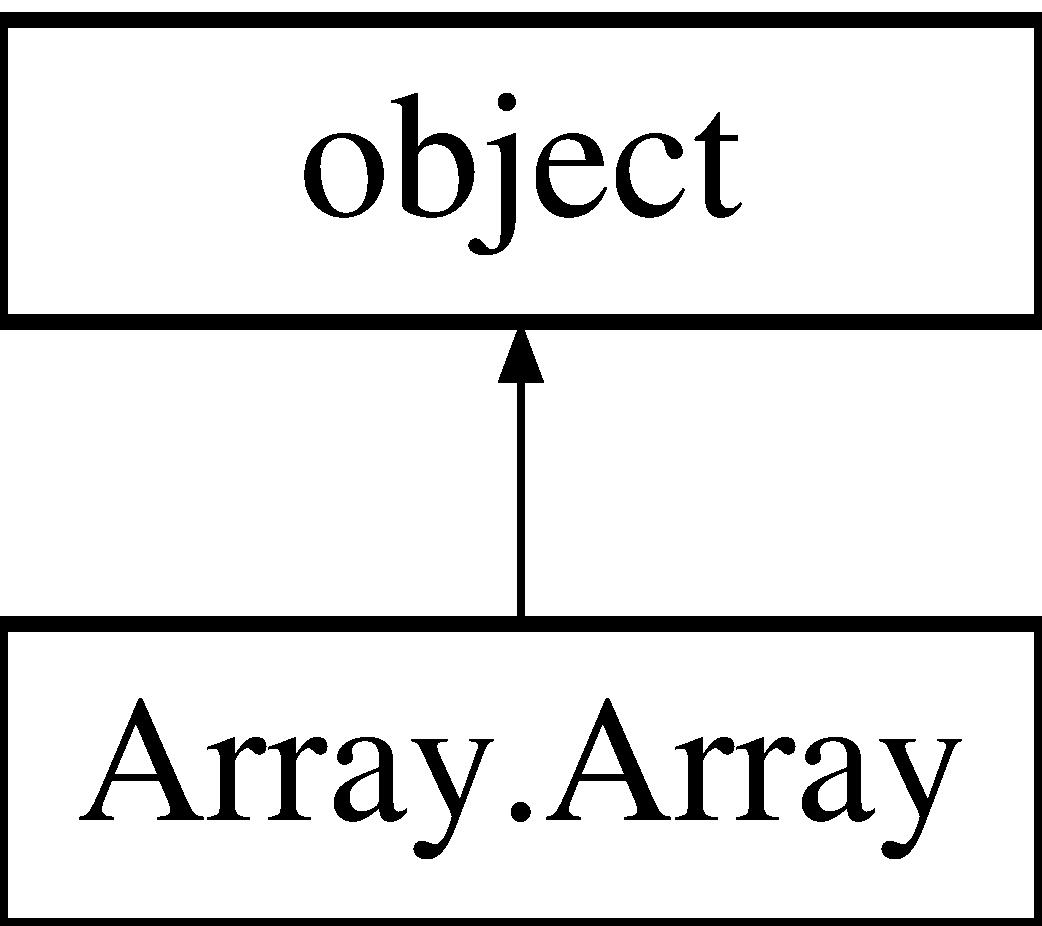
\includegraphics[height=2.000000cm]{class_array_1_1_array}
\end{center}
\end{figure}
\subsection*{Public Member Functions}
\begin{DoxyCompactItemize}
\item 
def \hyperlink{class_array_1_1_array_a35f27607f31ccfdede99590a30dc461c}{\+\_\+\+\_\+init\+\_\+\+\_\+}
\begin{DoxyCompactList}\small\item\em Construct a default array object. \end{DoxyCompactList}\item 
def \hyperlink{class_array_1_1_array_ab3a1e6afee220e0f6d2630836a0b7a0f}{get\+\_\+data\+\_\+structure\+\_\+type} (self)
\begin{DoxyCompactList}\small\item\em This method gets the data structure type. \end{DoxyCompactList}\item 
def \hyperlink{class_array_1_1_array_a5100331b1f7cb0448f235fd40d05f614}{set\+\_\+num\+\_\+dimensions} (self, nd)
\begin{DoxyCompactList}\small\item\em Set the number of dimensions of the array;. \end{DoxyCompactList}\item 
def \hyperlink{class_array_1_1_array_a237805bcdde6280bec65ebe0f68ce4e9}{get\+\_\+num\+\_\+dimensions} (self)
\begin{DoxyCompactList}\small\item\em Get the number of dimensions of the array;. \end{DoxyCompactList}\item 
def \hyperlink{class_array_1_1_array_afd27d06e12ffe980aa7e49d8a769dcf4}{set\+\_\+dimensions} (self, dim)
\begin{DoxyCompactList}\small\item\em Set the size of each dimensions; also allocates array space. \end{DoxyCompactList}\item 
def \hyperlink{class_array_1_1_array_a2cc5a41231b0dd595dc376d9463803bc}{get\+\_\+dimensions} (self, dim)
\begin{DoxyCompactList}\small\item\em Get the size of each dimensions;. \end{DoxyCompactList}\item 
def \hyperlink{class_array_1_1_array_a838c2a69bd0ddd3f15558aef3018dd36}{get\+\_\+size} (self)
\begin{DoxyCompactList}\small\item\em Get the array size. \end{DoxyCompactList}\item 
def \hyperlink{class_array_1_1_array_af6c128376f7da8e5c9d5cff376e91d27}{get\+\_\+element}
\item 
def \hyperlink{class_array_1_1_array_ae0ef8d2502f319fe5dd57b965b36bfe9}{set\+\_\+element}
\item 
def \hyperlink{class_array_1_1_array_a5185dc5446c5a4462ebb50ce92ffb755}{get\+\_\+value}
\begin{DoxyCompactList}\small\item\em Get the object at \textquotesingle{}indx\textquotesingle{}. \end{DoxyCompactList}\item 
def \hyperlink{class_array_1_1_array_a682f36ee39851758da013ae3d2e6708a}{set\+\_\+value}
\begin{DoxyCompactList}\small\item\em Set the input object at \textquotesingle{}indx\textquotesingle{}. \end{DoxyCompactList}\item 
def \hyperlink{class_array_1_1_array_aaceb6a3c839b2345d966f3815a3bd1cb}{get\+\_\+data\+\_\+structure\+\_\+representation} (self)
\begin{DoxyCompactList}\small\item\em Generating the J\+S\+O\+N string for a \hyperlink{namespace_bridges}{Bridges} array object (Array$<$\+E$>$\mbox{[}\mbox{]}) \end{DoxyCompactList}\end{DoxyCompactItemize}
\subsection*{Public Attributes}
\begin{DoxyCompactItemize}
\item 
\hyperlink{class_array_1_1_array_a75d2d3965f5232a430b069c8cce78d80}{array\+\_\+data}
\item 
\hyperlink{class_array_1_1_array_ad20e83f196d6ccc482e3d49adaeaaf71}{num\+\_\+dims}
\item 
\hyperlink{class_array_1_1_array_a421362e43ac706de326ea5442db7116b}{size}
\end{DoxyCompactItemize}
\subsection*{Static Public Attributes}
\begin{DoxyCompactItemize}
\item 
string \hyperlink{class_array_1_1_array_ae6bdb390ddba8126d3746296feccbf3a}{Q\+U\+O\+T\+E} = \char`\"{}\textbackslash{}\char`\"{}\char`\"{}
\item 
string \hyperlink{class_array_1_1_array_a050cf5fc5abfaee35b7960392d2a116f}{C\+O\+M\+M\+A} = \char`\"{},\char`\"{}
\item 
string \hyperlink{class_array_1_1_array_a9cd7f5a4340a676e8d7ec8a4fe6aaab7}{C\+O\+L\+O\+N} = \char`\"{}\+:\char`\"{}
\item 
string \hyperlink{class_array_1_1_array_a62203d6bf7e524eba3c9aaa28a139e2a}{O\+P\+E\+N\+\_\+\+C\+U\+R\+L\+Y} = \char`\"{}\{\char`\"{}
\item 
string \hyperlink{class_array_1_1_array_a36be40d3e5e79a0f0b541c170b8f2984}{C\+L\+O\+S\+E\+\_\+\+C\+U\+R\+L\+Y} = \char`\"{}\}\char`\"{}
\item 
string \hyperlink{class_array_1_1_array_ae1b619f58c038bca0e42114ec4afcd08}{O\+P\+E\+N\+\_\+\+P\+A\+R\+E\+N} = \char`\"{}(\char`\"{}
\item 
string \hyperlink{class_array_1_1_array_ac2b5bdf724baa7b645ffa0a569407213}{C\+L\+O\+S\+E\+\_\+\+P\+A\+R\+E\+N} = \char`\"{})\char`\"{}
\item 
string \hyperlink{class_array_1_1_array_a2bcecc8c5d787a739ec9bf8beb52fc77}{O\+P\+E\+N\+\_\+\+B\+O\+X} = \char`\"{}\mbox{[}\char`\"{}
\item 
string \hyperlink{class_array_1_1_array_ac8b79f827e1acec43ff2ddb4089abbe1}{C\+L\+O\+S\+E\+\_\+\+B\+O\+X} = \char`\"{}\mbox{]}\char`\"{}
\item 
list \hyperlink{class_array_1_1_array_aadd55f758422d491e4a6b51b3652f030}{array\+\_\+data} = \mbox{[}$\,$\mbox{]}
\item 
tuple \hyperlink{class_array_1_1_array_a3517087ba9c9e5bdc7e8cf4b0593decb}{num\+\_\+dims} = int()
\item 
list \hyperlink{class_array_1_1_array_ab0f0de822ea2ff937cbfbcf64081ff11}{dims} = \mbox{[}1, 1, 1\mbox{]}
\item 
tuple \hyperlink{class_array_1_1_array_ae605a16bf709991444aa703af03ef63d}{size} = int()
\end{DoxyCompactItemize}


\subsection{Detailed Description}
This class can be used to create arrays of type Element$<$\+E$>$. 

\begin{DoxyAuthor}{Author}
Kalpathi Subramanian
\end{DoxyAuthor}
\begin{DoxyDate}{Date}
10/8/16, 5/17/17
\end{DoxyDate}
This class can be used to create arrays of type Element$<$\+E$>$ where E is a generic object representing application specific data.

Arrays are internally represented as 1\+D arrays; currently 1\+D, 2\+D and 3\+D arrays are supported.


\begin{DoxyParams}{Parameters}
{\em $<$\+E$>$} & The generic parameter object that is part of this element, representing application specific data.\\
\hline
\end{DoxyParams}
\begin{DoxySeeAlso}{See also}
Example Tutorial at ~\newline
 \href{http://bridgesuncc.github.io/Hello_World_Tutorials/ARRAY1D.html}{\tt http\+://bridgesuncc.\+github.\+io/\+Hello\+\_\+\+World\+\_\+\+Tutorials/\+A\+R\+R\+A\+Y1\+D.\+html} (1\+D \hyperlink{class_array_1_1_array}{Array})~\newline
 \href{http://bridgesuncc.github.io/Hello_World_Tutorials/ARRAY2D.html}{\tt http\+://bridgesuncc.\+github.\+io/\+Hello\+\_\+\+World\+\_\+\+Tutorials/\+A\+R\+R\+A\+Y2\+D.\+html} (2\+D \hyperlink{class_array_1_1_array}{Array})~\newline
 \href{http://bridgesuncc.github.io/Hello_World_Tutorials/ARRAY3D.html}{\tt http\+://bridgesuncc.\+github.\+io/\+Hello\+\_\+\+World\+\_\+\+Tutorials/\+A\+R\+R\+A\+Y3\+D.\+html} (3\+D \hyperlink{class_array_1_1_array}{Array}) 
\end{DoxySeeAlso}


\subsection{Constructor \& Destructor Documentation}
\hypertarget{class_array_1_1_array_a35f27607f31ccfdede99590a30dc461c}{}\index{Array\+::\+Array@{Array\+::\+Array}!\+\_\+\+\_\+init\+\_\+\+\_\+@{\+\_\+\+\_\+init\+\_\+\+\_\+}}
\index{\+\_\+\+\_\+init\+\_\+\+\_\+@{\+\_\+\+\_\+init\+\_\+\+\_\+}!Array\+::\+Array@{Array\+::\+Array}}
\subsubsection[{\+\_\+\+\_\+init\+\_\+\+\_\+}]{\setlength{\rightskip}{0pt plus 5cm}def Array.\+Array.\+\_\+\+\_\+init\+\_\+\+\_\+ (
\begin{DoxyParamCaption}
\item[{}]{self, }
\item[{}]{num\+\_\+dims = {\ttfamily None}, }
\item[{}]{dims = {\ttfamily None}, }
\item[{}]{num\+\_\+elements = {\ttfamily None}, }
\item[{}]{x\+\_\+dim = {\ttfamily None}, }
\item[{}]{y\+\_\+dim = {\ttfamily None}, }
\item[{}]{z\+\_\+dim = {\ttfamily None}}
\end{DoxyParamCaption}
)}\label{class_array_1_1_array_a35f27607f31ccfdede99590a30dc461c}


Construct a default array object. 



\subsection{Member Function Documentation}
\hypertarget{class_array_1_1_array_aaceb6a3c839b2345d966f3815a3bd1cb}{}\index{Array\+::\+Array@{Array\+::\+Array}!get\+\_\+data\+\_\+structure\+\_\+representation@{get\+\_\+data\+\_\+structure\+\_\+representation}}
\index{get\+\_\+data\+\_\+structure\+\_\+representation@{get\+\_\+data\+\_\+structure\+\_\+representation}!Array\+::\+Array@{Array\+::\+Array}}
\subsubsection[{get\+\_\+data\+\_\+structure\+\_\+representation(self)}]{\setlength{\rightskip}{0pt plus 5cm}def Array.\+Array.\+get\+\_\+data\+\_\+structure\+\_\+representation (
\begin{DoxyParamCaption}
\item[{}]{self}
\end{DoxyParamCaption}
)}\label{class_array_1_1_array_aaceb6a3c839b2345d966f3815a3bd1cb}


Generating the J\+S\+O\+N string for a \hyperlink{namespace_bridges}{Bridges} array object (Array$<$\+E$>$\mbox{[}\mbox{]}) 


\begin{DoxyParams}{Parameters}
{\em \hyperlink{namespace_bridges}{Bridges}} & \hyperlink{class_array_1_1_array}{Array} object\\
\hline
\end{DoxyParams}
\begin{DoxyReturn}{Returns}
J\+S\+O\+N string 
\end{DoxyReturn}
\hypertarget{class_array_1_1_array_ab3a1e6afee220e0f6d2630836a0b7a0f}{}\index{Array\+::\+Array@{Array\+::\+Array}!get\+\_\+data\+\_\+structure\+\_\+type@{get\+\_\+data\+\_\+structure\+\_\+type}}
\index{get\+\_\+data\+\_\+structure\+\_\+type@{get\+\_\+data\+\_\+structure\+\_\+type}!Array\+::\+Array@{Array\+::\+Array}}
\subsubsection[{get\+\_\+data\+\_\+structure\+\_\+type(self)}]{\setlength{\rightskip}{0pt plus 5cm}def Array.\+Array.\+get\+\_\+data\+\_\+structure\+\_\+type (
\begin{DoxyParamCaption}
\item[{}]{self}
\end{DoxyParamCaption}
)}\label{class_array_1_1_array_ab3a1e6afee220e0f6d2630836a0b7a0f}


This method gets the data structure type. 

\begin{DoxyReturn}{Returns}
The date structure type as a string 
\end{DoxyReturn}
\hypertarget{class_array_1_1_array_a2cc5a41231b0dd595dc376d9463803bc}{}\index{Array\+::\+Array@{Array\+::\+Array}!get\+\_\+dimensions@{get\+\_\+dimensions}}
\index{get\+\_\+dimensions@{get\+\_\+dimensions}!Array\+::\+Array@{Array\+::\+Array}}
\subsubsection[{get\+\_\+dimensions(self, dim)}]{\setlength{\rightskip}{0pt plus 5cm}def Array.\+Array.\+get\+\_\+dimensions (
\begin{DoxyParamCaption}
\item[{}]{self, }
\item[{}]{dim}
\end{DoxyParamCaption}
)}\label{class_array_1_1_array_a2cc5a41231b0dd595dc376d9463803bc}


Get the size of each dimensions;. 


\begin{DoxyParams}{Parameters}
{\em dims\mbox{[}$\,$\mbox{]}} & size of each dimension is returned \\
\hline
\end{DoxyParams}
\hypertarget{class_array_1_1_array_af6c128376f7da8e5c9d5cff376e91d27}{}\index{Array\+::\+Array@{Array\+::\+Array}!get\+\_\+element@{get\+\_\+element}}
\index{get\+\_\+element@{get\+\_\+element}!Array\+::\+Array@{Array\+::\+Array}}
\subsubsection[{get\+\_\+element}]{\setlength{\rightskip}{0pt plus 5cm}def Array.\+Array.\+get\+\_\+element (
\begin{DoxyParamCaption}
\item[{}]{self, }
\item[{}]{indx = {\ttfamily None}, }
\item[{}]{x = {\ttfamily None}, }
\item[{}]{y = {\ttfamily None}, }
\item[{}]{z = {\ttfamily None}}
\end{DoxyParamCaption}
)}\label{class_array_1_1_array_af6c128376f7da8e5c9d5cff376e91d27}
\hypertarget{class_array_1_1_array_a237805bcdde6280bec65ebe0f68ce4e9}{}\index{Array\+::\+Array@{Array\+::\+Array}!get\+\_\+num\+\_\+dimensions@{get\+\_\+num\+\_\+dimensions}}
\index{get\+\_\+num\+\_\+dimensions@{get\+\_\+num\+\_\+dimensions}!Array\+::\+Array@{Array\+::\+Array}}
\subsubsection[{get\+\_\+num\+\_\+dimensions(self)}]{\setlength{\rightskip}{0pt plus 5cm}def Array.\+Array.\+get\+\_\+num\+\_\+dimensions (
\begin{DoxyParamCaption}
\item[{}]{self}
\end{DoxyParamCaption}
)}\label{class_array_1_1_array_a237805bcdde6280bec65ebe0f68ce4e9}


Get the number of dimensions of the array;. 

\begin{DoxyReturn}{Returns}
number of dimensions 
\end{DoxyReturn}
\hypertarget{class_array_1_1_array_a838c2a69bd0ddd3f15558aef3018dd36}{}\index{Array\+::\+Array@{Array\+::\+Array}!get\+\_\+size@{get\+\_\+size}}
\index{get\+\_\+size@{get\+\_\+size}!Array\+::\+Array@{Array\+::\+Array}}
\subsubsection[{get\+\_\+size(self)}]{\setlength{\rightskip}{0pt plus 5cm}def Array.\+Array.\+get\+\_\+size (
\begin{DoxyParamCaption}
\item[{}]{self}
\end{DoxyParamCaption}
)}\label{class_array_1_1_array_a838c2a69bd0ddd3f15558aef3018dd36}


Get the array size. 

\begin{DoxyReturn}{Returns}
size 
\end{DoxyReturn}
\hypertarget{class_array_1_1_array_a5185dc5446c5a4462ebb50ce92ffb755}{}\index{Array\+::\+Array@{Array\+::\+Array}!get\+\_\+value@{get\+\_\+value}}
\index{get\+\_\+value@{get\+\_\+value}!Array\+::\+Array@{Array\+::\+Array}}
\subsubsection[{get\+\_\+value}]{\setlength{\rightskip}{0pt plus 5cm}def Array.\+Array.\+get\+\_\+value (
\begin{DoxyParamCaption}
\item[{}]{self, }
\item[{}]{indx = {\ttfamily None}, }
\item[{}]{col = {\ttfamily None}, }
\item[{}]{row = {\ttfamily None}, }
\item[{}]{slice = {\ttfamily None}}
\end{DoxyParamCaption}
)}\label{class_array_1_1_array_a5185dc5446c5a4462ebb50ce92ffb755}


Get the object at \textquotesingle{}indx\textquotesingle{}. 


\begin{DoxyParams}{Parameters}
{\em indx} & index into the array \\
\hline
\end{DoxyParams}
\begin{DoxyReturn}{Returns}
Element$<$\+E$>$ object at \textquotesingle{}indx\textquotesingle{} 
\end{DoxyReturn}
\hypertarget{class_array_1_1_array_afd27d06e12ffe980aa7e49d8a769dcf4}{}\index{Array\+::\+Array@{Array\+::\+Array}!set\+\_\+dimensions@{set\+\_\+dimensions}}
\index{set\+\_\+dimensions@{set\+\_\+dimensions}!Array\+::\+Array@{Array\+::\+Array}}
\subsubsection[{set\+\_\+dimensions(self, dim)}]{\setlength{\rightskip}{0pt plus 5cm}def Array.\+Array.\+set\+\_\+dimensions (
\begin{DoxyParamCaption}
\item[{}]{self, }
\item[{}]{dim}
\end{DoxyParamCaption}
)}\label{class_array_1_1_array_afd27d06e12ffe980aa7e49d8a769dcf4}


Set the size of each dimensions; also allocates array space. 


\begin{DoxyParams}{Parameters}
{\em dim\mbox{[}$\,$\mbox{]}} & size of each dimension \\
\hline
\end{DoxyParams}
\hypertarget{class_array_1_1_array_ae0ef8d2502f319fe5dd57b965b36bfe9}{}\index{Array\+::\+Array@{Array\+::\+Array}!set\+\_\+element@{set\+\_\+element}}
\index{set\+\_\+element@{set\+\_\+element}!Array\+::\+Array@{Array\+::\+Array}}
\subsubsection[{set\+\_\+element}]{\setlength{\rightskip}{0pt plus 5cm}def Array.\+Array.\+set\+\_\+element (
\begin{DoxyParamCaption}
\item[{}]{self, }
\item[{}]{indx = {\ttfamily None}, }
\item[{}]{el = {\ttfamily None}, }
\item[{}]{x = {\ttfamily None}, }
\item[{}]{y = {\ttfamily None}, }
\item[{}]{z = {\ttfamily None}}
\end{DoxyParamCaption}
)}\label{class_array_1_1_array_ae0ef8d2502f319fe5dd57b965b36bfe9}
\hypertarget{class_array_1_1_array_a5100331b1f7cb0448f235fd40d05f614}{}\index{Array\+::\+Array@{Array\+::\+Array}!set\+\_\+num\+\_\+dimensions@{set\+\_\+num\+\_\+dimensions}}
\index{set\+\_\+num\+\_\+dimensions@{set\+\_\+num\+\_\+dimensions}!Array\+::\+Array@{Array\+::\+Array}}
\subsubsection[{set\+\_\+num\+\_\+dimensions(self, nd)}]{\setlength{\rightskip}{0pt plus 5cm}def Array.\+Array.\+set\+\_\+num\+\_\+dimensions (
\begin{DoxyParamCaption}
\item[{}]{self, }
\item[{}]{nd}
\end{DoxyParamCaption}
)}\label{class_array_1_1_array_a5100331b1f7cb0448f235fd40d05f614}


Set the number of dimensions of the array;. 


\begin{DoxyParams}{Parameters}
{\em nd} & number of dimensions \\
\hline
\end{DoxyParams}
\hypertarget{class_array_1_1_array_a682f36ee39851758da013ae3d2e6708a}{}\index{Array\+::\+Array@{Array\+::\+Array}!set\+\_\+value@{set\+\_\+value}}
\index{set\+\_\+value@{set\+\_\+value}!Array\+::\+Array@{Array\+::\+Array}}
\subsubsection[{set\+\_\+value}]{\setlength{\rightskip}{0pt plus 5cm}def Array.\+Array.\+set\+\_\+value (
\begin{DoxyParamCaption}
\item[{}]{self, }
\item[{}]{indx = {\ttfamily None}, }
\item[{}]{col = {\ttfamily None}, }
\item[{}]{row = {\ttfamily None}, }
\item[{}]{slice = {\ttfamily None}, }
\item[{}]{el = {\ttfamily None}}
\end{DoxyParamCaption}
)}\label{class_array_1_1_array_a682f36ee39851758da013ae3d2e6708a}


Set the input object at \textquotesingle{}indx\textquotesingle{}. 


\begin{DoxyParams}{Parameters}
{\em indx} & index into the array \\
\hline
{\em el} & element object to be assigned at \textquotesingle{}indx\textquotesingle{} \\
\hline
\end{DoxyParams}


\subsection{Member Data Documentation}
\hypertarget{class_array_1_1_array_aadd55f758422d491e4a6b51b3652f030}{}\index{Array\+::\+Array@{Array\+::\+Array}!array\+\_\+data@{array\+\_\+data}}
\index{array\+\_\+data@{array\+\_\+data}!Array\+::\+Array@{Array\+::\+Array}}
\subsubsection[{array\+\_\+data}]{\setlength{\rightskip}{0pt plus 5cm}list Array.\+Array.\+array\+\_\+data = \mbox{[}$\,$\mbox{]}\hspace{0.3cm}{\ttfamily [static]}}\label{class_array_1_1_array_aadd55f758422d491e4a6b51b3652f030}
\hypertarget{class_array_1_1_array_a75d2d3965f5232a430b069c8cce78d80}{}\index{Array\+::\+Array@{Array\+::\+Array}!array\+\_\+data@{array\+\_\+data}}
\index{array\+\_\+data@{array\+\_\+data}!Array\+::\+Array@{Array\+::\+Array}}
\subsubsection[{array\+\_\+data}]{\setlength{\rightskip}{0pt plus 5cm}Array.\+Array.\+array\+\_\+data}\label{class_array_1_1_array_a75d2d3965f5232a430b069c8cce78d80}
\hypertarget{class_array_1_1_array_ac8b79f827e1acec43ff2ddb4089abbe1}{}\index{Array\+::\+Array@{Array\+::\+Array}!C\+L\+O\+S\+E\+\_\+\+B\+O\+X@{C\+L\+O\+S\+E\+\_\+\+B\+O\+X}}
\index{C\+L\+O\+S\+E\+\_\+\+B\+O\+X@{C\+L\+O\+S\+E\+\_\+\+B\+O\+X}!Array\+::\+Array@{Array\+::\+Array}}
\subsubsection[{C\+L\+O\+S\+E\+\_\+\+B\+O\+X}]{\setlength{\rightskip}{0pt plus 5cm}string Array.\+Array.\+C\+L\+O\+S\+E\+\_\+\+B\+O\+X = \char`\"{}\mbox{]}\char`\"{}\hspace{0.3cm}{\ttfamily [static]}}\label{class_array_1_1_array_ac8b79f827e1acec43ff2ddb4089abbe1}
\hypertarget{class_array_1_1_array_a36be40d3e5e79a0f0b541c170b8f2984}{}\index{Array\+::\+Array@{Array\+::\+Array}!C\+L\+O\+S\+E\+\_\+\+C\+U\+R\+L\+Y@{C\+L\+O\+S\+E\+\_\+\+C\+U\+R\+L\+Y}}
\index{C\+L\+O\+S\+E\+\_\+\+C\+U\+R\+L\+Y@{C\+L\+O\+S\+E\+\_\+\+C\+U\+R\+L\+Y}!Array\+::\+Array@{Array\+::\+Array}}
\subsubsection[{C\+L\+O\+S\+E\+\_\+\+C\+U\+R\+L\+Y}]{\setlength{\rightskip}{0pt plus 5cm}string Array.\+Array.\+C\+L\+O\+S\+E\+\_\+\+C\+U\+R\+L\+Y = \char`\"{}\}\char`\"{}\hspace{0.3cm}{\ttfamily [static]}}\label{class_array_1_1_array_a36be40d3e5e79a0f0b541c170b8f2984}
\hypertarget{class_array_1_1_array_ac2b5bdf724baa7b645ffa0a569407213}{}\index{Array\+::\+Array@{Array\+::\+Array}!C\+L\+O\+S\+E\+\_\+\+P\+A\+R\+E\+N@{C\+L\+O\+S\+E\+\_\+\+P\+A\+R\+E\+N}}
\index{C\+L\+O\+S\+E\+\_\+\+P\+A\+R\+E\+N@{C\+L\+O\+S\+E\+\_\+\+P\+A\+R\+E\+N}!Array\+::\+Array@{Array\+::\+Array}}
\subsubsection[{C\+L\+O\+S\+E\+\_\+\+P\+A\+R\+E\+N}]{\setlength{\rightskip}{0pt plus 5cm}string Array.\+Array.\+C\+L\+O\+S\+E\+\_\+\+P\+A\+R\+E\+N = \char`\"{})\char`\"{}\hspace{0.3cm}{\ttfamily [static]}}\label{class_array_1_1_array_ac2b5bdf724baa7b645ffa0a569407213}
\hypertarget{class_array_1_1_array_a9cd7f5a4340a676e8d7ec8a4fe6aaab7}{}\index{Array\+::\+Array@{Array\+::\+Array}!C\+O\+L\+O\+N@{C\+O\+L\+O\+N}}
\index{C\+O\+L\+O\+N@{C\+O\+L\+O\+N}!Array\+::\+Array@{Array\+::\+Array}}
\subsubsection[{C\+O\+L\+O\+N}]{\setlength{\rightskip}{0pt plus 5cm}string Array.\+Array.\+C\+O\+L\+O\+N = \char`\"{}\+:\char`\"{}\hspace{0.3cm}{\ttfamily [static]}}\label{class_array_1_1_array_a9cd7f5a4340a676e8d7ec8a4fe6aaab7}
\hypertarget{class_array_1_1_array_a050cf5fc5abfaee35b7960392d2a116f}{}\index{Array\+::\+Array@{Array\+::\+Array}!C\+O\+M\+M\+A@{C\+O\+M\+M\+A}}
\index{C\+O\+M\+M\+A@{C\+O\+M\+M\+A}!Array\+::\+Array@{Array\+::\+Array}}
\subsubsection[{C\+O\+M\+M\+A}]{\setlength{\rightskip}{0pt plus 5cm}string Array.\+Array.\+C\+O\+M\+M\+A = \char`\"{},\char`\"{}\hspace{0.3cm}{\ttfamily [static]}}\label{class_array_1_1_array_a050cf5fc5abfaee35b7960392d2a116f}
\hypertarget{class_array_1_1_array_ab0f0de822ea2ff937cbfbcf64081ff11}{}\index{Array\+::\+Array@{Array\+::\+Array}!dims@{dims}}
\index{dims@{dims}!Array\+::\+Array@{Array\+::\+Array}}
\subsubsection[{dims}]{\setlength{\rightskip}{0pt plus 5cm}list Array.\+Array.\+dims = \mbox{[}1, 1, 1\mbox{]}\hspace{0.3cm}{\ttfamily [static]}}\label{class_array_1_1_array_ab0f0de822ea2ff937cbfbcf64081ff11}
\hypertarget{class_array_1_1_array_a3517087ba9c9e5bdc7e8cf4b0593decb}{}\index{Array\+::\+Array@{Array\+::\+Array}!num\+\_\+dims@{num\+\_\+dims}}
\index{num\+\_\+dims@{num\+\_\+dims}!Array\+::\+Array@{Array\+::\+Array}}
\subsubsection[{num\+\_\+dims}]{\setlength{\rightskip}{0pt plus 5cm}tuple Array.\+Array.\+num\+\_\+dims = int()\hspace{0.3cm}{\ttfamily [static]}}\label{class_array_1_1_array_a3517087ba9c9e5bdc7e8cf4b0593decb}
\hypertarget{class_array_1_1_array_ad20e83f196d6ccc482e3d49adaeaaf71}{}\index{Array\+::\+Array@{Array\+::\+Array}!num\+\_\+dims@{num\+\_\+dims}}
\index{num\+\_\+dims@{num\+\_\+dims}!Array\+::\+Array@{Array\+::\+Array}}
\subsubsection[{num\+\_\+dims}]{\setlength{\rightskip}{0pt plus 5cm}Array.\+Array.\+num\+\_\+dims}\label{class_array_1_1_array_ad20e83f196d6ccc482e3d49adaeaaf71}
\hypertarget{class_array_1_1_array_a2bcecc8c5d787a739ec9bf8beb52fc77}{}\index{Array\+::\+Array@{Array\+::\+Array}!O\+P\+E\+N\+\_\+\+B\+O\+X@{O\+P\+E\+N\+\_\+\+B\+O\+X}}
\index{O\+P\+E\+N\+\_\+\+B\+O\+X@{O\+P\+E\+N\+\_\+\+B\+O\+X}!Array\+::\+Array@{Array\+::\+Array}}
\subsubsection[{O\+P\+E\+N\+\_\+\+B\+O\+X}]{\setlength{\rightskip}{0pt plus 5cm}string Array.\+Array.\+O\+P\+E\+N\+\_\+\+B\+O\+X = \char`\"{}\mbox{[}\char`\"{}\hspace{0.3cm}{\ttfamily [static]}}\label{class_array_1_1_array_a2bcecc8c5d787a739ec9bf8beb52fc77}
\hypertarget{class_array_1_1_array_a62203d6bf7e524eba3c9aaa28a139e2a}{}\index{Array\+::\+Array@{Array\+::\+Array}!O\+P\+E\+N\+\_\+\+C\+U\+R\+L\+Y@{O\+P\+E\+N\+\_\+\+C\+U\+R\+L\+Y}}
\index{O\+P\+E\+N\+\_\+\+C\+U\+R\+L\+Y@{O\+P\+E\+N\+\_\+\+C\+U\+R\+L\+Y}!Array\+::\+Array@{Array\+::\+Array}}
\subsubsection[{O\+P\+E\+N\+\_\+\+C\+U\+R\+L\+Y}]{\setlength{\rightskip}{0pt plus 5cm}string Array.\+Array.\+O\+P\+E\+N\+\_\+\+C\+U\+R\+L\+Y = \char`\"{}\{\char`\"{}\hspace{0.3cm}{\ttfamily [static]}}\label{class_array_1_1_array_a62203d6bf7e524eba3c9aaa28a139e2a}
\hypertarget{class_array_1_1_array_ae1b619f58c038bca0e42114ec4afcd08}{}\index{Array\+::\+Array@{Array\+::\+Array}!O\+P\+E\+N\+\_\+\+P\+A\+R\+E\+N@{O\+P\+E\+N\+\_\+\+P\+A\+R\+E\+N}}
\index{O\+P\+E\+N\+\_\+\+P\+A\+R\+E\+N@{O\+P\+E\+N\+\_\+\+P\+A\+R\+E\+N}!Array\+::\+Array@{Array\+::\+Array}}
\subsubsection[{O\+P\+E\+N\+\_\+\+P\+A\+R\+E\+N}]{\setlength{\rightskip}{0pt plus 5cm}string Array.\+Array.\+O\+P\+E\+N\+\_\+\+P\+A\+R\+E\+N = \char`\"{}(\char`\"{}\hspace{0.3cm}{\ttfamily [static]}}\label{class_array_1_1_array_ae1b619f58c038bca0e42114ec4afcd08}
\hypertarget{class_array_1_1_array_ae6bdb390ddba8126d3746296feccbf3a}{}\index{Array\+::\+Array@{Array\+::\+Array}!Q\+U\+O\+T\+E@{Q\+U\+O\+T\+E}}
\index{Q\+U\+O\+T\+E@{Q\+U\+O\+T\+E}!Array\+::\+Array@{Array\+::\+Array}}
\subsubsection[{Q\+U\+O\+T\+E}]{\setlength{\rightskip}{0pt plus 5cm}string Array.\+Array.\+Q\+U\+O\+T\+E = \char`\"{}\textbackslash{}\char`\"{}\char`\"{}\hspace{0.3cm}{\ttfamily [static]}}\label{class_array_1_1_array_ae6bdb390ddba8126d3746296feccbf3a}
\hypertarget{class_array_1_1_array_ae605a16bf709991444aa703af03ef63d}{}\index{Array\+::\+Array@{Array\+::\+Array}!size@{size}}
\index{size@{size}!Array\+::\+Array@{Array\+::\+Array}}
\subsubsection[{size}]{\setlength{\rightskip}{0pt plus 5cm}tuple Array.\+Array.\+size = int()\hspace{0.3cm}{\ttfamily [static]}}\label{class_array_1_1_array_ae605a16bf709991444aa703af03ef63d}
\hypertarget{class_array_1_1_array_a421362e43ac706de326ea5442db7116b}{}\index{Array\+::\+Array@{Array\+::\+Array}!size@{size}}
\index{size@{size}!Array\+::\+Array@{Array\+::\+Array}}
\subsubsection[{size}]{\setlength{\rightskip}{0pt plus 5cm}Array.\+Array.\+size}\label{class_array_1_1_array_a421362e43ac706de326ea5442db7116b}


The documentation for this class was generated from the following file\+:\begin{DoxyCompactItemize}
\item 
/\+Users/krs/gr/bridges/bridges17/python/src/\hyperlink{_array_8py}{Array.\+py}\end{DoxyCompactItemize}

\hypertarget{class_a_v_l_tree_element_1_1_a_v_l_tree_element}{}\section{A\+V\+L\+Tree\+Element.\+A\+V\+L\+Tree\+Element Class Reference}
\label{class_a_v_l_tree_element_1_1_a_v_l_tree_element}\index{A\+V\+L\+Tree\+Element.\+A\+V\+L\+Tree\+Element@{A\+V\+L\+Tree\+Element.\+A\+V\+L\+Tree\+Element}}


This class extends the \hyperlink{namespace_b_s_t_element}{B\+S\+T\+Element} class by adding a height and balance factor fields that are useful in A\+V\+L trees.  


Inheritance diagram for A\+V\+L\+Tree\+Element.\+A\+V\+L\+Tree\+Element\+:\begin{figure}[H]
\begin{center}
\leavevmode
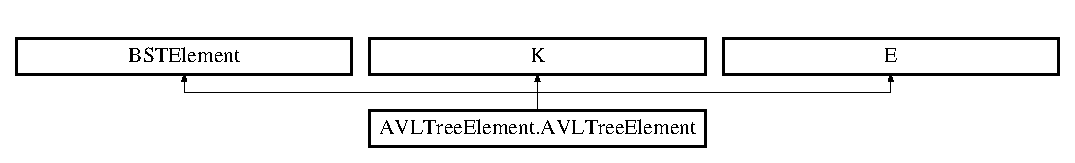
\includegraphics[height=6.000000cm]{class_a_v_l_tree_element_1_1_a_v_l_tree_element}
\end{center}
\end{figure}
\subsection*{Public Member Functions}
\begin{DoxyCompactItemize}
\item 
def \hyperlink{class_a_v_l_tree_element_1_1_a_v_l_tree_element_a696c8654b851172b6918728a3e47631c}{\+\_\+\+\_\+init\+\_\+\+\_\+}
\begin{DoxyCompactList}\small\item\em Construct an \hyperlink{class_a_v_l_tree_element_1_1_a_v_l_tree_element}{A\+V\+L\+Tree\+Element} with default values. \end{DoxyCompactList}\item 
def \hyperlink{class_a_v_l_tree_element_1_1_a_v_l_tree_element_af1dd46ba9ec315666b049ae3647d6f28}{get\+\_\+data\+\_\+structure\+\_\+type} (self)
\begin{DoxyCompactList}\small\item\em This method gets the data structure type. \end{DoxyCompactList}\item 
def \hyperlink{class_a_v_l_tree_element_1_1_a_v_l_tree_element_ac2feaad2712bc0a592e02e14c775e987}{get\+\_\+height} (self)
\begin{DoxyCompactList}\small\item\em This method returns the height of the tree at this node. \end{DoxyCompactList}\item 
def \hyperlink{class_a_v_l_tree_element_1_1_a_v_l_tree_element_af61b40eaf63816f7737fb4da69d6d6b0}{set\+\_\+height} (self, h)
\begin{DoxyCompactList}\small\item\em This method sets the height of the tree at this node. \end{DoxyCompactList}\item 
def \hyperlink{class_a_v_l_tree_element_1_1_a_v_l_tree_element_ac4d2c2c91b8b44f7af1699f3d0e498a2}{get\+\_\+balance\+\_\+factor} (self)
\begin{DoxyCompactList}\small\item\em This method returns the balance factor of the tree at this node. \end{DoxyCompactList}\item 
def \hyperlink{class_a_v_l_tree_element_1_1_a_v_l_tree_element_ae57a5a7dd74ddf0b15e281e9cfdb6192}{set\+\_\+balance\+\_\+factor} (self, bf)
\begin{DoxyCompactList}\small\item\em This method sets the balance factor of the tree at this node. \end{DoxyCompactList}\item 
def \hyperlink{class_a_v_l_tree_element_1_1_a_v_l_tree_element_a448b7a53957a85982ef36e1e828bab4a}{get\+\_\+left} (self)
\begin{DoxyCompactList}\small\item\em This method returns the left child of the tree node. \end{DoxyCompactList}\item 
def \hyperlink{class_a_v_l_tree_element_1_1_a_v_l_tree_element_a07ac5fd29a29b8020e8826c9d00f4a48}{get\+\_\+\+Right} (self)
\begin{DoxyCompactList}\small\item\em This method returns the right child of tree node. \end{DoxyCompactList}\end{DoxyCompactItemize}
\subsection*{Public Attributes}
\begin{DoxyCompactItemize}
\item 
\hyperlink{class_a_v_l_tree_element_1_1_a_v_l_tree_element_acf75c045d479489e7a3add1b547d2624}{height}
\item 
\hyperlink{class_a_v_l_tree_element_1_1_a_v_l_tree_element_a9e11a9ae47fe02077ad1597be21e5403}{bal\+\_\+factor}
\end{DoxyCompactItemize}
\subsection*{Static Public Attributes}
\begin{DoxyCompactItemize}
\item 
tuple \hyperlink{class_a_v_l_tree_element_1_1_a_v_l_tree_element_a6af5676b71ccb44e0f7e1b5a26cd9afc}{height} = int()
\item 
tuple \hyperlink{class_a_v_l_tree_element_1_1_a_v_l_tree_element_a8e6fed7c8e6a2ca9ced0b9289a28fa68}{bal\+\_\+factor} = int()
\end{DoxyCompactItemize}


\subsection{Detailed Description}
This class extends the \hyperlink{namespace_b_s_t_element}{B\+S\+T\+Element} class by adding a height and balance factor fields that are useful in A\+V\+L trees. 

A\+V\+L tree elements include a \textquotesingle{}height\textquotesingle{} and a \textquotesingle{}bal\+Factor\textquotesingle{} value, representing the height and balance factor of the A\+V\+L tree at that node, respectively. This is useful in representing A\+V\+L trees.

A\+V\+L\+Tree elements contain a visualizer (\hyperlink{namespace_element_visualizer}{Element\+Visualizer}) object for setting visual attributes (color, shape, opacity, size), necessary for displaying them in a web browser.

A\+V\+L\+Tree elements also have a \hyperlink{namespace_link_visualizer}{Link\+Visualizer} object, that is used when they are linked to another element, appropriate for setting link attributes, for instance, between $\ast$ the current element and its left or right child


\begin{DoxyParams}{Parameters}
{\em E} & he generic parameter object that is part of this element, representing application specific data. \\
\hline
{\em K} & is the search key parameter in the A\+V\+L tree node; K must be orderable, such as integer, float, string, etc., on which relational operators work.\\
\hline
\end{DoxyParams}
\begin{DoxyAuthor}{Author}
Kalpathi Subramanian, Mihai Mehedint
\end{DoxyAuthor}
\begin{DoxyDate}{Date}
6/22/16, 1/7/17, 5/17/17
\end{DoxyDate}
\begin{DoxySeeAlso}{See also}
Example tutorial using \hyperlink{class_a_v_l_tree_element_1_1_a_v_l_tree_element}{A\+V\+L\+Tree\+Element} at ~\newline
 \href{http://bridgesuncc.github.io/Hello_World_Tutorials/AVL.html}{\tt http\+://bridgesuncc.\+github.\+io/\+Hello\+\_\+\+World\+\_\+\+Tutorials/\+A\+V\+L.\+html} 
\end{DoxySeeAlso}


\subsection{Constructor \& Destructor Documentation}
\hypertarget{class_a_v_l_tree_element_1_1_a_v_l_tree_element_a696c8654b851172b6918728a3e47631c}{}\index{A\+V\+L\+Tree\+Element\+::\+A\+V\+L\+Tree\+Element@{A\+V\+L\+Tree\+Element\+::\+A\+V\+L\+Tree\+Element}!\+\_\+\+\_\+init\+\_\+\+\_\+@{\+\_\+\+\_\+init\+\_\+\+\_\+}}
\index{\+\_\+\+\_\+init\+\_\+\+\_\+@{\+\_\+\+\_\+init\+\_\+\+\_\+}!A\+V\+L\+Tree\+Element\+::\+A\+V\+L\+Tree\+Element@{A\+V\+L\+Tree\+Element\+::\+A\+V\+L\+Tree\+Element}}
\subsubsection[{\+\_\+\+\_\+init\+\_\+\+\_\+}]{\setlength{\rightskip}{0pt plus 5cm}def A\+V\+L\+Tree\+Element.\+A\+V\+L\+Tree\+Element.\+\_\+\+\_\+init\+\_\+\+\_\+ (
\begin{DoxyParamCaption}
\item[{}]{self, }
\item[{}]{k = {\ttfamily None}, }
\item[{}]{e = {\ttfamily None}}
\end{DoxyParamCaption}
)}\label{class_a_v_l_tree_element_1_1_a_v_l_tree_element_a696c8654b851172b6918728a3e47631c}


Construct an \hyperlink{class_a_v_l_tree_element_1_1_a_v_l_tree_element}{A\+V\+L\+Tree\+Element} with default values. 



\subsection{Member Function Documentation}
\hypertarget{class_a_v_l_tree_element_1_1_a_v_l_tree_element_ac4d2c2c91b8b44f7af1699f3d0e498a2}{}\index{A\+V\+L\+Tree\+Element\+::\+A\+V\+L\+Tree\+Element@{A\+V\+L\+Tree\+Element\+::\+A\+V\+L\+Tree\+Element}!get\+\_\+balance\+\_\+factor@{get\+\_\+balance\+\_\+factor}}
\index{get\+\_\+balance\+\_\+factor@{get\+\_\+balance\+\_\+factor}!A\+V\+L\+Tree\+Element\+::\+A\+V\+L\+Tree\+Element@{A\+V\+L\+Tree\+Element\+::\+A\+V\+L\+Tree\+Element}}
\subsubsection[{get\+\_\+balance\+\_\+factor(self)}]{\setlength{\rightskip}{0pt plus 5cm}def A\+V\+L\+Tree\+Element.\+A\+V\+L\+Tree\+Element.\+get\+\_\+balance\+\_\+factor (
\begin{DoxyParamCaption}
\item[{}]{self}
\end{DoxyParamCaption}
)}\label{class_a_v_l_tree_element_1_1_a_v_l_tree_element_ac4d2c2c91b8b44f7af1699f3d0e498a2}


This method returns the balance factor of the tree at this node. 

\begin{DoxyReturn}{Returns}
balance factor 
\end{DoxyReturn}
\hypertarget{class_a_v_l_tree_element_1_1_a_v_l_tree_element_af1dd46ba9ec315666b049ae3647d6f28}{}\index{A\+V\+L\+Tree\+Element\+::\+A\+V\+L\+Tree\+Element@{A\+V\+L\+Tree\+Element\+::\+A\+V\+L\+Tree\+Element}!get\+\_\+data\+\_\+structure\+\_\+type@{get\+\_\+data\+\_\+structure\+\_\+type}}
\index{get\+\_\+data\+\_\+structure\+\_\+type@{get\+\_\+data\+\_\+structure\+\_\+type}!A\+V\+L\+Tree\+Element\+::\+A\+V\+L\+Tree\+Element@{A\+V\+L\+Tree\+Element\+::\+A\+V\+L\+Tree\+Element}}
\subsubsection[{get\+\_\+data\+\_\+structure\+\_\+type(self)}]{\setlength{\rightskip}{0pt plus 5cm}def A\+V\+L\+Tree\+Element.\+A\+V\+L\+Tree\+Element.\+get\+\_\+data\+\_\+structure\+\_\+type (
\begin{DoxyParamCaption}
\item[{}]{self}
\end{DoxyParamCaption}
)}\label{class_a_v_l_tree_element_1_1_a_v_l_tree_element_af1dd46ba9ec315666b049ae3647d6f28}


This method gets the data structure type. 

\begin{DoxyReturn}{Returns}
The date structure type as a string 
\end{DoxyReturn}
\hypertarget{class_a_v_l_tree_element_1_1_a_v_l_tree_element_ac2feaad2712bc0a592e02e14c775e987}{}\index{A\+V\+L\+Tree\+Element\+::\+A\+V\+L\+Tree\+Element@{A\+V\+L\+Tree\+Element\+::\+A\+V\+L\+Tree\+Element}!get\+\_\+height@{get\+\_\+height}}
\index{get\+\_\+height@{get\+\_\+height}!A\+V\+L\+Tree\+Element\+::\+A\+V\+L\+Tree\+Element@{A\+V\+L\+Tree\+Element\+::\+A\+V\+L\+Tree\+Element}}
\subsubsection[{get\+\_\+height(self)}]{\setlength{\rightskip}{0pt plus 5cm}def A\+V\+L\+Tree\+Element.\+A\+V\+L\+Tree\+Element.\+get\+\_\+height (
\begin{DoxyParamCaption}
\item[{}]{self}
\end{DoxyParamCaption}
)}\label{class_a_v_l_tree_element_1_1_a_v_l_tree_element_ac2feaad2712bc0a592e02e14c775e987}


This method returns the height of the tree at this node. 

\begin{DoxyReturn}{Returns}
height 
\end{DoxyReturn}
\hypertarget{class_a_v_l_tree_element_1_1_a_v_l_tree_element_a448b7a53957a85982ef36e1e828bab4a}{}\index{A\+V\+L\+Tree\+Element\+::\+A\+V\+L\+Tree\+Element@{A\+V\+L\+Tree\+Element\+::\+A\+V\+L\+Tree\+Element}!get\+\_\+left@{get\+\_\+left}}
\index{get\+\_\+left@{get\+\_\+left}!A\+V\+L\+Tree\+Element\+::\+A\+V\+L\+Tree\+Element@{A\+V\+L\+Tree\+Element\+::\+A\+V\+L\+Tree\+Element}}
\subsubsection[{get\+\_\+left(self)}]{\setlength{\rightskip}{0pt plus 5cm}def A\+V\+L\+Tree\+Element.\+A\+V\+L\+Tree\+Element.\+get\+\_\+left (
\begin{DoxyParamCaption}
\item[{}]{self}
\end{DoxyParamCaption}
)}\label{class_a_v_l_tree_element_1_1_a_v_l_tree_element_a448b7a53957a85982ef36e1e828bab4a}


This method returns the left child of the tree node. 

\begin{DoxyReturn}{Returns}
the left child of this node 
\end{DoxyReturn}
\hypertarget{class_a_v_l_tree_element_1_1_a_v_l_tree_element_a07ac5fd29a29b8020e8826c9d00f4a48}{}\index{A\+V\+L\+Tree\+Element\+::\+A\+V\+L\+Tree\+Element@{A\+V\+L\+Tree\+Element\+::\+A\+V\+L\+Tree\+Element}!get\+\_\+\+Right@{get\+\_\+\+Right}}
\index{get\+\_\+\+Right@{get\+\_\+\+Right}!A\+V\+L\+Tree\+Element\+::\+A\+V\+L\+Tree\+Element@{A\+V\+L\+Tree\+Element\+::\+A\+V\+L\+Tree\+Element}}
\subsubsection[{get\+\_\+\+Right(self)}]{\setlength{\rightskip}{0pt plus 5cm}def A\+V\+L\+Tree\+Element.\+A\+V\+L\+Tree\+Element.\+get\+\_\+\+Right (
\begin{DoxyParamCaption}
\item[{}]{self}
\end{DoxyParamCaption}
)}\label{class_a_v_l_tree_element_1_1_a_v_l_tree_element_a07ac5fd29a29b8020e8826c9d00f4a48}


This method returns the right child of tree node. 

\begin{DoxyReturn}{Returns}
the right child of this node 
\end{DoxyReturn}
\hypertarget{class_a_v_l_tree_element_1_1_a_v_l_tree_element_ae57a5a7dd74ddf0b15e281e9cfdb6192}{}\index{A\+V\+L\+Tree\+Element\+::\+A\+V\+L\+Tree\+Element@{A\+V\+L\+Tree\+Element\+::\+A\+V\+L\+Tree\+Element}!set\+\_\+balance\+\_\+factor@{set\+\_\+balance\+\_\+factor}}
\index{set\+\_\+balance\+\_\+factor@{set\+\_\+balance\+\_\+factor}!A\+V\+L\+Tree\+Element\+::\+A\+V\+L\+Tree\+Element@{A\+V\+L\+Tree\+Element\+::\+A\+V\+L\+Tree\+Element}}
\subsubsection[{set\+\_\+balance\+\_\+factor(self, bf)}]{\setlength{\rightskip}{0pt plus 5cm}def A\+V\+L\+Tree\+Element.\+A\+V\+L\+Tree\+Element.\+set\+\_\+balance\+\_\+factor (
\begin{DoxyParamCaption}
\item[{}]{self, }
\item[{}]{bf}
\end{DoxyParamCaption}
)}\label{class_a_v_l_tree_element_1_1_a_v_l_tree_element_ae57a5a7dd74ddf0b15e281e9cfdb6192}


This method sets the balance factor of the tree at this node. 


\begin{DoxyParams}{Parameters}
{\em balance} & factor bf \\
\hline
\end{DoxyParams}
\hypertarget{class_a_v_l_tree_element_1_1_a_v_l_tree_element_af61b40eaf63816f7737fb4da69d6d6b0}{}\index{A\+V\+L\+Tree\+Element\+::\+A\+V\+L\+Tree\+Element@{A\+V\+L\+Tree\+Element\+::\+A\+V\+L\+Tree\+Element}!set\+\_\+height@{set\+\_\+height}}
\index{set\+\_\+height@{set\+\_\+height}!A\+V\+L\+Tree\+Element\+::\+A\+V\+L\+Tree\+Element@{A\+V\+L\+Tree\+Element\+::\+A\+V\+L\+Tree\+Element}}
\subsubsection[{set\+\_\+height(self, h)}]{\setlength{\rightskip}{0pt plus 5cm}def A\+V\+L\+Tree\+Element.\+A\+V\+L\+Tree\+Element.\+set\+\_\+height (
\begin{DoxyParamCaption}
\item[{}]{self, }
\item[{}]{h}
\end{DoxyParamCaption}
)}\label{class_a_v_l_tree_element_1_1_a_v_l_tree_element_af61b40eaf63816f7737fb4da69d6d6b0}


This method sets the height of the tree at this node. 


\begin{DoxyParams}{Parameters}
{\em height} & h \\
\hline
\end{DoxyParams}


\subsection{Member Data Documentation}
\hypertarget{class_a_v_l_tree_element_1_1_a_v_l_tree_element_a8e6fed7c8e6a2ca9ced0b9289a28fa68}{}\index{A\+V\+L\+Tree\+Element\+::\+A\+V\+L\+Tree\+Element@{A\+V\+L\+Tree\+Element\+::\+A\+V\+L\+Tree\+Element}!bal\+\_\+factor@{bal\+\_\+factor}}
\index{bal\+\_\+factor@{bal\+\_\+factor}!A\+V\+L\+Tree\+Element\+::\+A\+V\+L\+Tree\+Element@{A\+V\+L\+Tree\+Element\+::\+A\+V\+L\+Tree\+Element}}
\subsubsection[{bal\+\_\+factor}]{\setlength{\rightskip}{0pt plus 5cm}tuple A\+V\+L\+Tree\+Element.\+A\+V\+L\+Tree\+Element.\+bal\+\_\+factor = int()\hspace{0.3cm}{\ttfamily [static]}}\label{class_a_v_l_tree_element_1_1_a_v_l_tree_element_a8e6fed7c8e6a2ca9ced0b9289a28fa68}
\hypertarget{class_a_v_l_tree_element_1_1_a_v_l_tree_element_a9e11a9ae47fe02077ad1597be21e5403}{}\index{A\+V\+L\+Tree\+Element\+::\+A\+V\+L\+Tree\+Element@{A\+V\+L\+Tree\+Element\+::\+A\+V\+L\+Tree\+Element}!bal\+\_\+factor@{bal\+\_\+factor}}
\index{bal\+\_\+factor@{bal\+\_\+factor}!A\+V\+L\+Tree\+Element\+::\+A\+V\+L\+Tree\+Element@{A\+V\+L\+Tree\+Element\+::\+A\+V\+L\+Tree\+Element}}
\subsubsection[{bal\+\_\+factor}]{\setlength{\rightskip}{0pt plus 5cm}A\+V\+L\+Tree\+Element.\+A\+V\+L\+Tree\+Element.\+bal\+\_\+factor}\label{class_a_v_l_tree_element_1_1_a_v_l_tree_element_a9e11a9ae47fe02077ad1597be21e5403}
\hypertarget{class_a_v_l_tree_element_1_1_a_v_l_tree_element_a6af5676b71ccb44e0f7e1b5a26cd9afc}{}\index{A\+V\+L\+Tree\+Element\+::\+A\+V\+L\+Tree\+Element@{A\+V\+L\+Tree\+Element\+::\+A\+V\+L\+Tree\+Element}!height@{height}}
\index{height@{height}!A\+V\+L\+Tree\+Element\+::\+A\+V\+L\+Tree\+Element@{A\+V\+L\+Tree\+Element\+::\+A\+V\+L\+Tree\+Element}}
\subsubsection[{height}]{\setlength{\rightskip}{0pt plus 5cm}tuple A\+V\+L\+Tree\+Element.\+A\+V\+L\+Tree\+Element.\+height = int()\hspace{0.3cm}{\ttfamily [static]}}\label{class_a_v_l_tree_element_1_1_a_v_l_tree_element_a6af5676b71ccb44e0f7e1b5a26cd9afc}
\hypertarget{class_a_v_l_tree_element_1_1_a_v_l_tree_element_acf75c045d479489e7a3add1b547d2624}{}\index{A\+V\+L\+Tree\+Element\+::\+A\+V\+L\+Tree\+Element@{A\+V\+L\+Tree\+Element\+::\+A\+V\+L\+Tree\+Element}!height@{height}}
\index{height@{height}!A\+V\+L\+Tree\+Element\+::\+A\+V\+L\+Tree\+Element@{A\+V\+L\+Tree\+Element\+::\+A\+V\+L\+Tree\+Element}}
\subsubsection[{height}]{\setlength{\rightskip}{0pt plus 5cm}A\+V\+L\+Tree\+Element.\+A\+V\+L\+Tree\+Element.\+height}\label{class_a_v_l_tree_element_1_1_a_v_l_tree_element_acf75c045d479489e7a3add1b547d2624}


The documentation for this class was generated from the following file\+:\begin{DoxyCompactItemize}
\item 
/\+Users/krs/gr/bridges/bridges17/python/src/\hyperlink{_a_v_l_tree_element_8py}{A\+V\+L\+Tree\+Element.\+py}\end{DoxyCompactItemize}

\hypertarget{class_bin_tree_element_1_1_bin_tree_element}{}\section{Bin\+Tree\+Element.\+Bin\+Tree\+Element Class Reference}
\label{class_bin_tree_element_1_1_bin_tree_element}\index{Bin\+Tree\+Element.\+Bin\+Tree\+Element@{Bin\+Tree\+Element.\+Bin\+Tree\+Element}}


This class is extended from the Tree\+Element class and can be used to create binary tree element objects.  


Inheritance diagram for Bin\+Tree\+Element.\+Bin\+Tree\+Element\+:\begin{figure}[H]
\begin{center}
\leavevmode
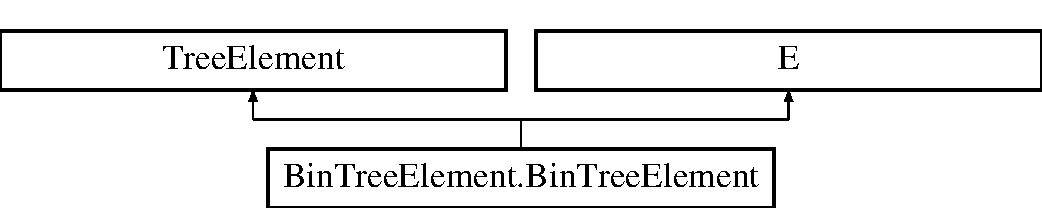
\includegraphics[height=2.000000cm]{class_bin_tree_element_1_1_bin_tree_element}
\end{center}
\end{figure}
\subsection*{Public Member Functions}
\begin{DoxyCompactItemize}
\item 
def \hyperlink{class_bin_tree_element_1_1_bin_tree_element_a9a6be9d4770ea3113e0e622b0d71a035}{\+\_\+\+\_\+init\+\_\+\+\_\+} (self)
\begin{DoxyCompactList}\small\item\em Constructs an empty Binary Tree \hyperlink{namespace_element}{Element} with right and left pointers set to null. \end{DoxyCompactList}\item 
def \hyperlink{class_bin_tree_element_1_1_bin_tree_element_a74e275475f366145d4987458ad08841b}{get\+Data\+Struct\+Type} (self)
\begin{DoxyCompactList}\small\item\em This method gets the data structure type. \end{DoxyCompactList}\item 
def \hyperlink{class_bin_tree_element_1_1_bin_tree_element_a8515226277b5632baf3f0a57c0095fa6}{get\+Left} (self)
\begin{DoxyCompactList}\small\item\em This method returns the left tree element pointer. \end{DoxyCompactList}\item 
def \hyperlink{class_bin_tree_element_1_1_bin_tree_element_a9d8856b4d16a7ba680ad699cc4328cd6}{set\+Left} (self, \hyperlink{class_bin_tree_element_1_1_bin_tree_element_a73a75929ad5c317a59915283866ddb7a}{left})
\begin{DoxyCompactList}\small\item\em This method sets the left tree element pointer. \end{DoxyCompactList}\item 
def \hyperlink{class_bin_tree_element_1_1_bin_tree_element_a292647759d9bd7f705e6240afed1b707}{get\+Right} (self)
\begin{DoxyCompactList}\small\item\em This method returns the right tree element pointer. \end{DoxyCompactList}\item 
def \hyperlink{class_bin_tree_element_1_1_bin_tree_element_a64f9dabb9089c9fd5b94a6cc6c262944}{set\+Right} (self, \hyperlink{class_bin_tree_element_1_1_bin_tree_element_a9e5201df4cc9cc2a970b35ba036bca5a}{right})
\begin{DoxyCompactList}\small\item\em This method sets the right tree element pointer. \end{DoxyCompactList}\end{DoxyCompactItemize}
\subsection*{Static Public Attributes}
\begin{DoxyCompactItemize}
\item 
\hyperlink{class_bin_tree_element_1_1_bin_tree_element_a73a75929ad5c317a59915283866ddb7a}{left} = \hyperlink{class_bin_tree_element_1_1_bin_tree_element}{Bin\+Tree\+Element}()
\item 
\hyperlink{class_bin_tree_element_1_1_bin_tree_element_a9e5201df4cc9cc2a970b35ba036bca5a}{right} = \hyperlink{class_bin_tree_element_1_1_bin_tree_element}{Bin\+Tree\+Element}()
\end{DoxyCompactItemize}


\subsection{Detailed Description}
This class is extended from the Tree\+Element class and can be used to create binary tree element objects. 

The Bin\+Tree element class is the building block for creating binary tree structures. It contains two children (viz., left, right).

\hyperlink{class_bin_tree_element_1_1_bin_tree_element}{Bin\+Tree\+Element} contains a visualizer (\hyperlink{namespace_element_visualizer}{Element\+Visualizer}) object for setting visual attributes (color, shape, opacity, size), necessary for displaying them in a web browser.

Elements also have a \hyperlink{namespace_link_visualizer}{Link\+Visualizer} object, that is used when they are linked to another element, appropriate for setting link attributes, for instance, between the current element and its left or right child


\begin{DoxyParams}{Parameters}
{\em E} & he generic parameter object that is part of this element, representing application specific data.\\
\hline
\end{DoxyParams}
\begin{DoxyAuthor}{Author}
Kalpathi Subramanian, Mihai Mehedint
\end{DoxyAuthor}
\begin{DoxyDate}{Date}
6/22/16, 1/7/17, 5/17/17
\end{DoxyDate}
\begin{DoxySeeAlso}{See also}
Example Tutorial at ~\newline
 \href{http://bridgesuncc.github.io/Hello_World_Tutorials/BTree.html@verbatim}{\tt http\+://bridgesuncc.\+github.\+io/\+Hello\+\_\+\+World\+\_\+\+Tutorials/\+B\+Tree.\+html@verbatim} generated source for class \hyperlink{class_bin_tree_element_1_1_bin_tree_element}{Bin\+Tree\+Element}  
\end{DoxySeeAlso}


\subsection{Constructor \& Destructor Documentation}
\hypertarget{class_bin_tree_element_1_1_bin_tree_element_a9a6be9d4770ea3113e0e622b0d71a035}{}\label{class_bin_tree_element_1_1_bin_tree_element_a9a6be9d4770ea3113e0e622b0d71a035} 
\index{Bin\+Tree\+Element\+::\+Bin\+Tree\+Element@{Bin\+Tree\+Element\+::\+Bin\+Tree\+Element}!\+\_\+\+\_\+init\+\_\+\+\_\+@{\+\_\+\+\_\+init\+\_\+\+\_\+}}
\index{\+\_\+\+\_\+init\+\_\+\+\_\+@{\+\_\+\+\_\+init\+\_\+\+\_\+}!Bin\+Tree\+Element\+::\+Bin\+Tree\+Element@{Bin\+Tree\+Element\+::\+Bin\+Tree\+Element}}
\subsubsection{\texorpdfstring{\+\_\+\+\_\+init\+\_\+\+\_\+()}{\_\_init\_\_()}}
{\footnotesize\ttfamily def Bin\+Tree\+Element.\+Bin\+Tree\+Element.\+\_\+\+\_\+init\+\_\+\+\_\+ (\begin{DoxyParamCaption}\item[{}]{self }\end{DoxyParamCaption})}



Constructs an empty Binary Tree \hyperlink{namespace_element}{Element} with right and left pointers set to null. 

\begin{DoxyVerb}generated source for method __init__ \end{DoxyVerb}
 

\subsection{Member Function Documentation}
\hypertarget{class_bin_tree_element_1_1_bin_tree_element_a74e275475f366145d4987458ad08841b}{}\label{class_bin_tree_element_1_1_bin_tree_element_a74e275475f366145d4987458ad08841b} 
\index{Bin\+Tree\+Element\+::\+Bin\+Tree\+Element@{Bin\+Tree\+Element\+::\+Bin\+Tree\+Element}!get\+Data\+Struct\+Type@{get\+Data\+Struct\+Type}}
\index{get\+Data\+Struct\+Type@{get\+Data\+Struct\+Type}!Bin\+Tree\+Element\+::\+Bin\+Tree\+Element@{Bin\+Tree\+Element\+::\+Bin\+Tree\+Element}}
\subsubsection{\texorpdfstring{get\+Data\+Struct\+Type()}{getDataStructType()}}
{\footnotesize\ttfamily def Bin\+Tree\+Element.\+Bin\+Tree\+Element.\+get\+Data\+Struct\+Type (\begin{DoxyParamCaption}\item[{}]{self }\end{DoxyParamCaption})}



This method gets the data structure type. 

\begin{DoxyReturn}{Returns}
The date structure type as a string\begin{DoxyVerb}generated source for method getDataStructType \end{DoxyVerb}
 
\end{DoxyReturn}
\hypertarget{class_bin_tree_element_1_1_bin_tree_element_a8515226277b5632baf3f0a57c0095fa6}{}\label{class_bin_tree_element_1_1_bin_tree_element_a8515226277b5632baf3f0a57c0095fa6} 
\index{Bin\+Tree\+Element\+::\+Bin\+Tree\+Element@{Bin\+Tree\+Element\+::\+Bin\+Tree\+Element}!get\+Left@{get\+Left}}
\index{get\+Left@{get\+Left}!Bin\+Tree\+Element\+::\+Bin\+Tree\+Element@{Bin\+Tree\+Element\+::\+Bin\+Tree\+Element}}
\subsubsection{\texorpdfstring{get\+Left()}{getLeft()}}
{\footnotesize\ttfamily def Bin\+Tree\+Element.\+Bin\+Tree\+Element.\+get\+Left (\begin{DoxyParamCaption}\item[{}]{self }\end{DoxyParamCaption})}



This method returns the left tree element pointer. 

\begin{DoxyReturn}{Returns}
the left child of this Tree\+Element\begin{DoxyVerb}generated source for method getLeft \end{DoxyVerb}
 
\end{DoxyReturn}
\hypertarget{class_bin_tree_element_1_1_bin_tree_element_a292647759d9bd7f705e6240afed1b707}{}\label{class_bin_tree_element_1_1_bin_tree_element_a292647759d9bd7f705e6240afed1b707} 
\index{Bin\+Tree\+Element\+::\+Bin\+Tree\+Element@{Bin\+Tree\+Element\+::\+Bin\+Tree\+Element}!get\+Right@{get\+Right}}
\index{get\+Right@{get\+Right}!Bin\+Tree\+Element\+::\+Bin\+Tree\+Element@{Bin\+Tree\+Element\+::\+Bin\+Tree\+Element}}
\subsubsection{\texorpdfstring{get\+Right()}{getRight()}}
{\footnotesize\ttfamily def Bin\+Tree\+Element.\+Bin\+Tree\+Element.\+get\+Right (\begin{DoxyParamCaption}\item[{}]{self }\end{DoxyParamCaption})}



This method returns the right tree element pointer. 

\begin{DoxyReturn}{Returns}
the right child of this Tree\+Element\begin{DoxyVerb}generated source for method getRight \end{DoxyVerb}
 
\end{DoxyReturn}
\hypertarget{class_bin_tree_element_1_1_bin_tree_element_a9d8856b4d16a7ba680ad699cc4328cd6}{}\label{class_bin_tree_element_1_1_bin_tree_element_a9d8856b4d16a7ba680ad699cc4328cd6} 
\index{Bin\+Tree\+Element\+::\+Bin\+Tree\+Element@{Bin\+Tree\+Element\+::\+Bin\+Tree\+Element}!set\+Left@{set\+Left}}
\index{set\+Left@{set\+Left}!Bin\+Tree\+Element\+::\+Bin\+Tree\+Element@{Bin\+Tree\+Element\+::\+Bin\+Tree\+Element}}
\subsubsection{\texorpdfstring{set\+Left()}{setLeft()}}
{\footnotesize\ttfamily def Bin\+Tree\+Element.\+Bin\+Tree\+Element.\+set\+Left (\begin{DoxyParamCaption}\item[{}]{self,  }\item[{}]{left }\end{DoxyParamCaption})}



This method sets the left tree element pointer. 


\begin{DoxyParams}{Parameters}
{\em left} & the Tree\+Element that should be assigned to the left child\begin{DoxyVerb}generated source for method setLeft \end{DoxyVerb}
 \\
\hline
\end{DoxyParams}
\hypertarget{class_bin_tree_element_1_1_bin_tree_element_a64f9dabb9089c9fd5b94a6cc6c262944}{}\label{class_bin_tree_element_1_1_bin_tree_element_a64f9dabb9089c9fd5b94a6cc6c262944} 
\index{Bin\+Tree\+Element\+::\+Bin\+Tree\+Element@{Bin\+Tree\+Element\+::\+Bin\+Tree\+Element}!set\+Right@{set\+Right}}
\index{set\+Right@{set\+Right}!Bin\+Tree\+Element\+::\+Bin\+Tree\+Element@{Bin\+Tree\+Element\+::\+Bin\+Tree\+Element}}
\subsubsection{\texorpdfstring{set\+Right()}{setRight()}}
{\footnotesize\ttfamily def Bin\+Tree\+Element.\+Bin\+Tree\+Element.\+set\+Right (\begin{DoxyParamCaption}\item[{}]{self,  }\item[{}]{right }\end{DoxyParamCaption})}



This method sets the right tree element pointer. 


\begin{DoxyParams}{Parameters}
{\em right} & the Tree\+Element that should be assigned to the right child\begin{DoxyVerb}generated source for method setRight \end{DoxyVerb}
 \\
\hline
\end{DoxyParams}


\subsection{Member Data Documentation}
\hypertarget{class_bin_tree_element_1_1_bin_tree_element_a73a75929ad5c317a59915283866ddb7a}{}\label{class_bin_tree_element_1_1_bin_tree_element_a73a75929ad5c317a59915283866ddb7a} 
\index{Bin\+Tree\+Element\+::\+Bin\+Tree\+Element@{Bin\+Tree\+Element\+::\+Bin\+Tree\+Element}!left@{left}}
\index{left@{left}!Bin\+Tree\+Element\+::\+Bin\+Tree\+Element@{Bin\+Tree\+Element\+::\+Bin\+Tree\+Element}}
\subsubsection{\texorpdfstring{left}{left}}
{\footnotesize\ttfamily Bin\+Tree\+Element.\+Bin\+Tree\+Element.\+left = \hyperlink{class_bin_tree_element_1_1_bin_tree_element}{Bin\+Tree\+Element}()\hspace{0.3cm}{\ttfamily [static]}}

\hypertarget{class_bin_tree_element_1_1_bin_tree_element_a9e5201df4cc9cc2a970b35ba036bca5a}{}\label{class_bin_tree_element_1_1_bin_tree_element_a9e5201df4cc9cc2a970b35ba036bca5a} 
\index{Bin\+Tree\+Element\+::\+Bin\+Tree\+Element@{Bin\+Tree\+Element\+::\+Bin\+Tree\+Element}!right@{right}}
\index{right@{right}!Bin\+Tree\+Element\+::\+Bin\+Tree\+Element@{Bin\+Tree\+Element\+::\+Bin\+Tree\+Element}}
\subsubsection{\texorpdfstring{right}{right}}
{\footnotesize\ttfamily Bin\+Tree\+Element.\+Bin\+Tree\+Element.\+right = \hyperlink{class_bin_tree_element_1_1_bin_tree_element}{Bin\+Tree\+Element}()\hspace{0.3cm}{\ttfamily [static]}}



The documentation for this class was generated from the following file\+:\begin{DoxyCompactItemize}
\item 
/\+Users/kalpathi/gr/bridges/client/python/src/\hyperlink{_bin_tree_element_8py}{Bin\+Tree\+Element.\+py}\end{DoxyCompactItemize}

\hypertarget{class_book_1_1_book}{}\section{Book.\+Book Class Reference}
\label{class_book_1_1_book}\index{Book.\+Book@{Book.\+Book}}
\subsection*{Public Member Functions}
\begin{DoxyCompactItemize}
\item 
def \hyperlink{class_book_1_1_book_a636c49cc5d000c29413a407452d32816}{\+\_\+\+\_\+init\+\_\+\+\_\+} (self, \hyperlink{class_book_1_1_book_a89a361c254d917406ee551760572ff19}{author\+Name}, \hyperlink{class_book_1_1_book_a969f0a0875741882763cb5d801277ebe}{author\+Birth}, \hyperlink{class_book_1_1_book_a4cca4f7acae85aef123dab48548d3b69}{author\+Death}, \hyperlink{class_book_1_1_book_aae1eab64f0e054709c003a270e86a202}{title}, \hyperlink{class_book_1_1_book_a00802108d115f37bf17f6fc5170022e9}{lang}, \hyperlink{class_book_1_1_book_a9e831408f7aa45b9cf66b10613cfaf31}{genre}, \hyperlink{class_book_1_1_book_a84be9f573910fda354e34de00fc95a61}{subject}, \hyperlink{class_book_1_1_book_ad3086167cb5f89b8f4de240a00ae64bc}{num\+Chars}, \hyperlink{class_book_1_1_book_accd8ca17020fbb9dc73b7a0b3d9348e2}{num\+Words}, \hyperlink{class_book_1_1_book_a750700b9cc757c9b23ab2c5030731543}{num\+Sentences}, \hyperlink{class_book_1_1_book_a87b247900d6c59f9a7ad179ad4214148}{num\+Difficult\+Words}, \hyperlink{class_book_1_1_book_a365ef43a762948ef862841d4d2f46420}{url}, downloads)
\item 
def \hyperlink{class_book_1_1_book_ab7cc9694c4c3df2f768f943385ac2886}{get\+Author\+Name} (self)
\item 
def \hyperlink{class_book_1_1_book_a7c53e0f893947ccddf6c1b166dd2beb5}{set\+Author\+Name} (self, \hyperlink{class_book_1_1_book_a89a361c254d917406ee551760572ff19}{author\+Name})
\item 
def \hyperlink{class_book_1_1_book_adba9746e2eb95129acabcbf18557a67f}{get\+Author\+Birth} (self)
\item 
def \hyperlink{class_book_1_1_book_a14279c2bd5b0e4e9c5c4bcd49369027a}{set\+Author\+Birth} (self, \hyperlink{class_book_1_1_book_a969f0a0875741882763cb5d801277ebe}{author\+Birth})
\item 
def \hyperlink{class_book_1_1_book_a8e8a1a282b92b869ee849f59ebfb55fd}{get\+Author\+Death} (self)
\item 
def \hyperlink{class_book_1_1_book_aa9ac68023cb24e8bf3bb550e0a52b72b}{set\+Author\+Death} (self, \hyperlink{class_book_1_1_book_a4cca4f7acae85aef123dab48548d3b69}{author\+Death})
\item 
def \hyperlink{class_book_1_1_book_a1a727d9ff491390e1f412550a0a1a085}{get\+Title} (self)
\item 
def \hyperlink{class_book_1_1_book_a7e6d14f5ef76084a2cc4968a6508789e}{set\+Title} (self, \hyperlink{class_book_1_1_book_aae1eab64f0e054709c003a270e86a202}{title})
\item 
def \hyperlink{class_book_1_1_book_aa80fb9893fb613f60a4d4f6b9aae6578}{get\+Lang} (self)
\item 
def \hyperlink{class_book_1_1_book_a473260171cdda228c3dc4ab1abced390}{set\+Lang} (self, \hyperlink{class_book_1_1_book_a00802108d115f37bf17f6fc5170022e9}{lang})
\item 
def \hyperlink{class_book_1_1_book_a03451826cf3a6a2843d27099a75d5334}{get\+Genre} (self)
\item 
def \hyperlink{class_book_1_1_book_a4056207d0b08cd67fda4c72507226cee}{set\+Genre} (self, \hyperlink{class_book_1_1_book_a9e831408f7aa45b9cf66b10613cfaf31}{genre})
\item 
def \hyperlink{class_book_1_1_book_af2c578b6367c85a4c1d532055b520192}{get\+Subject} (self)
\item 
def \hyperlink{class_book_1_1_book_a8f4ec300d24d5a6e9f6664d1860058c8}{set\+Subject} (self, \hyperlink{class_book_1_1_book_a84be9f573910fda354e34de00fc95a61}{subject})
\item 
def \hyperlink{class_book_1_1_book_a60c57a7b990ee481e7e8d3efafc950d9}{get\+U\+R\+L} (self)
\item 
def \hyperlink{class_book_1_1_book_a49214cdce23b923775b544b8e0fc3ba3}{set\+U\+R\+L} (self, \hyperlink{class_book_1_1_book_a365ef43a762948ef862841d4d2f46420}{url})
\item 
def \hyperlink{class_book_1_1_book_a5cd9079f12d86718f9df8e566f5c88d3}{get\+Num\+Chars} (self)
\item 
def \hyperlink{class_book_1_1_book_ae7a0206c29fb9e175abb51ce595c86a4}{set\+Num\+Chars} (self, \hyperlink{class_book_1_1_book_ad3086167cb5f89b8f4de240a00ae64bc}{num\+Chars})
\item 
def \hyperlink{class_book_1_1_book_a8352f92d15b66fd4c4aebd619ce05baa}{get\+Num\+Words} (self)
\item 
def \hyperlink{class_book_1_1_book_a8beb8c69d484c2a0e4c63116be3ba3f1}{set\+Num\+Words} (self, \hyperlink{class_book_1_1_book_accd8ca17020fbb9dc73b7a0b3d9348e2}{num\+Words})
\item 
def \hyperlink{class_book_1_1_book_a6edddaa897389c0250f51d8a6a392262}{get\+Num\+Sentences} (self)
\item 
def \hyperlink{class_book_1_1_book_aeac3717984fd8576a23f2784d879a89d}{set\+Num\+Sentences} (self, \hyperlink{class_book_1_1_book_a750700b9cc757c9b23ab2c5030731543}{num\+Sentences})
\item 
def \hyperlink{class_book_1_1_book_aa5a3abf812d967bae0f53a16ec878330}{get\+Num\+Difficult\+Words} (self)
\item 
def \hyperlink{class_book_1_1_book_a1fbc22c45b29980164469329a492b8fd}{set\+Num\+Difficult\+Words} (self, \hyperlink{class_book_1_1_book_a87b247900d6c59f9a7ad179ad4214148}{num\+Difficult\+Words})
\end{DoxyCompactItemize}
\subsection*{Public Attributes}
\begin{DoxyCompactItemize}
\item 
\hyperlink{class_book_1_1_book_a89a361c254d917406ee551760572ff19}{author\+Name}
\item 
\hyperlink{class_book_1_1_book_a969f0a0875741882763cb5d801277ebe}{author\+Birth}
\item 
\hyperlink{class_book_1_1_book_a4cca4f7acae85aef123dab48548d3b69}{author\+Death}
\item 
\hyperlink{class_book_1_1_book_aae1eab64f0e054709c003a270e86a202}{title}
\item 
\hyperlink{class_book_1_1_book_a00802108d115f37bf17f6fc5170022e9}{lang}
\item 
\hyperlink{class_book_1_1_book_a9e831408f7aa45b9cf66b10613cfaf31}{genre}
\item 
\hyperlink{class_book_1_1_book_a84be9f573910fda354e34de00fc95a61}{subject}
\item 
\hyperlink{class_book_1_1_book_a365ef43a762948ef862841d4d2f46420}{url}
\item 
\hyperlink{class_book_1_1_book_ad3086167cb5f89b8f4de240a00ae64bc}{num\+Chars}
\item 
\hyperlink{class_book_1_1_book_accd8ca17020fbb9dc73b7a0b3d9348e2}{num\+Words}
\item 
\hyperlink{class_book_1_1_book_a750700b9cc757c9b23ab2c5030731543}{num\+Sentences}
\item 
\hyperlink{class_book_1_1_book_a87b247900d6c59f9a7ad179ad4214148}{num\+Difficult\+Words}
\end{DoxyCompactItemize}


\subsection{Constructor \& Destructor Documentation}
\hypertarget{class_book_1_1_book_a636c49cc5d000c29413a407452d32816}{}\index{Book\+::\+Book@{Book\+::\+Book}!\+\_\+\+\_\+init\+\_\+\+\_\+@{\+\_\+\+\_\+init\+\_\+\+\_\+}}
\index{\+\_\+\+\_\+init\+\_\+\+\_\+@{\+\_\+\+\_\+init\+\_\+\+\_\+}!Book\+::\+Book@{Book\+::\+Book}}
\subsubsection[{\+\_\+\+\_\+init\+\_\+\+\_\+(self, author\+Name, author\+Birth, author\+Death, title, lang, genre, subject, num\+Chars, num\+Words, num\+Sentences, num\+Difficult\+Words, url, downloads)}]{\setlength{\rightskip}{0pt plus 5cm}def Book.\+Book.\+\_\+\+\_\+init\+\_\+\+\_\+ (
\begin{DoxyParamCaption}
\item[{}]{self, }
\item[{}]{author\+Name, }
\item[{}]{author\+Birth, }
\item[{}]{author\+Death, }
\item[{}]{title, }
\item[{}]{lang, }
\item[{}]{genre, }
\item[{}]{subject, }
\item[{}]{num\+Chars, }
\item[{}]{num\+Words, }
\item[{}]{num\+Sentences, }
\item[{}]{num\+Difficult\+Words, }
\item[{}]{url, }
\item[{}]{downloads}
\end{DoxyParamCaption}
)}\label{class_book_1_1_book_a636c49cc5d000c29413a407452d32816}


\subsection{Member Function Documentation}
\hypertarget{class_book_1_1_book_adba9746e2eb95129acabcbf18557a67f}{}\index{Book\+::\+Book@{Book\+::\+Book}!get\+Author\+Birth@{get\+Author\+Birth}}
\index{get\+Author\+Birth@{get\+Author\+Birth}!Book\+::\+Book@{Book\+::\+Book}}
\subsubsection[{get\+Author\+Birth(self)}]{\setlength{\rightskip}{0pt plus 5cm}def Book.\+Book.\+get\+Author\+Birth (
\begin{DoxyParamCaption}
\item[{}]{self}
\end{DoxyParamCaption}
)}\label{class_book_1_1_book_adba9746e2eb95129acabcbf18557a67f}
\hypertarget{class_book_1_1_book_a8e8a1a282b92b869ee849f59ebfb55fd}{}\index{Book\+::\+Book@{Book\+::\+Book}!get\+Author\+Death@{get\+Author\+Death}}
\index{get\+Author\+Death@{get\+Author\+Death}!Book\+::\+Book@{Book\+::\+Book}}
\subsubsection[{get\+Author\+Death(self)}]{\setlength{\rightskip}{0pt plus 5cm}def Book.\+Book.\+get\+Author\+Death (
\begin{DoxyParamCaption}
\item[{}]{self}
\end{DoxyParamCaption}
)}\label{class_book_1_1_book_a8e8a1a282b92b869ee849f59ebfb55fd}
\hypertarget{class_book_1_1_book_ab7cc9694c4c3df2f768f943385ac2886}{}\index{Book\+::\+Book@{Book\+::\+Book}!get\+Author\+Name@{get\+Author\+Name}}
\index{get\+Author\+Name@{get\+Author\+Name}!Book\+::\+Book@{Book\+::\+Book}}
\subsubsection[{get\+Author\+Name(self)}]{\setlength{\rightskip}{0pt plus 5cm}def Book.\+Book.\+get\+Author\+Name (
\begin{DoxyParamCaption}
\item[{}]{self}
\end{DoxyParamCaption}
)}\label{class_book_1_1_book_ab7cc9694c4c3df2f768f943385ac2886}
\hypertarget{class_book_1_1_book_a03451826cf3a6a2843d27099a75d5334}{}\index{Book\+::\+Book@{Book\+::\+Book}!get\+Genre@{get\+Genre}}
\index{get\+Genre@{get\+Genre}!Book\+::\+Book@{Book\+::\+Book}}
\subsubsection[{get\+Genre(self)}]{\setlength{\rightskip}{0pt plus 5cm}def Book.\+Book.\+get\+Genre (
\begin{DoxyParamCaption}
\item[{}]{self}
\end{DoxyParamCaption}
)}\label{class_book_1_1_book_a03451826cf3a6a2843d27099a75d5334}
\hypertarget{class_book_1_1_book_aa80fb9893fb613f60a4d4f6b9aae6578}{}\index{Book\+::\+Book@{Book\+::\+Book}!get\+Lang@{get\+Lang}}
\index{get\+Lang@{get\+Lang}!Book\+::\+Book@{Book\+::\+Book}}
\subsubsection[{get\+Lang(self)}]{\setlength{\rightskip}{0pt plus 5cm}def Book.\+Book.\+get\+Lang (
\begin{DoxyParamCaption}
\item[{}]{self}
\end{DoxyParamCaption}
)}\label{class_book_1_1_book_aa80fb9893fb613f60a4d4f6b9aae6578}
\hypertarget{class_book_1_1_book_a5cd9079f12d86718f9df8e566f5c88d3}{}\index{Book\+::\+Book@{Book\+::\+Book}!get\+Num\+Chars@{get\+Num\+Chars}}
\index{get\+Num\+Chars@{get\+Num\+Chars}!Book\+::\+Book@{Book\+::\+Book}}
\subsubsection[{get\+Num\+Chars(self)}]{\setlength{\rightskip}{0pt plus 5cm}def Book.\+Book.\+get\+Num\+Chars (
\begin{DoxyParamCaption}
\item[{}]{self}
\end{DoxyParamCaption}
)}\label{class_book_1_1_book_a5cd9079f12d86718f9df8e566f5c88d3}
\hypertarget{class_book_1_1_book_aa5a3abf812d967bae0f53a16ec878330}{}\index{Book\+::\+Book@{Book\+::\+Book}!get\+Num\+Difficult\+Words@{get\+Num\+Difficult\+Words}}
\index{get\+Num\+Difficult\+Words@{get\+Num\+Difficult\+Words}!Book\+::\+Book@{Book\+::\+Book}}
\subsubsection[{get\+Num\+Difficult\+Words(self)}]{\setlength{\rightskip}{0pt plus 5cm}def Book.\+Book.\+get\+Num\+Difficult\+Words (
\begin{DoxyParamCaption}
\item[{}]{self}
\end{DoxyParamCaption}
)}\label{class_book_1_1_book_aa5a3abf812d967bae0f53a16ec878330}
\hypertarget{class_book_1_1_book_a6edddaa897389c0250f51d8a6a392262}{}\index{Book\+::\+Book@{Book\+::\+Book}!get\+Num\+Sentences@{get\+Num\+Sentences}}
\index{get\+Num\+Sentences@{get\+Num\+Sentences}!Book\+::\+Book@{Book\+::\+Book}}
\subsubsection[{get\+Num\+Sentences(self)}]{\setlength{\rightskip}{0pt plus 5cm}def Book.\+Book.\+get\+Num\+Sentences (
\begin{DoxyParamCaption}
\item[{}]{self}
\end{DoxyParamCaption}
)}\label{class_book_1_1_book_a6edddaa897389c0250f51d8a6a392262}
\hypertarget{class_book_1_1_book_a8352f92d15b66fd4c4aebd619ce05baa}{}\index{Book\+::\+Book@{Book\+::\+Book}!get\+Num\+Words@{get\+Num\+Words}}
\index{get\+Num\+Words@{get\+Num\+Words}!Book\+::\+Book@{Book\+::\+Book}}
\subsubsection[{get\+Num\+Words(self)}]{\setlength{\rightskip}{0pt plus 5cm}def Book.\+Book.\+get\+Num\+Words (
\begin{DoxyParamCaption}
\item[{}]{self}
\end{DoxyParamCaption}
)}\label{class_book_1_1_book_a8352f92d15b66fd4c4aebd619ce05baa}
\hypertarget{class_book_1_1_book_af2c578b6367c85a4c1d532055b520192}{}\index{Book\+::\+Book@{Book\+::\+Book}!get\+Subject@{get\+Subject}}
\index{get\+Subject@{get\+Subject}!Book\+::\+Book@{Book\+::\+Book}}
\subsubsection[{get\+Subject(self)}]{\setlength{\rightskip}{0pt plus 5cm}def Book.\+Book.\+get\+Subject (
\begin{DoxyParamCaption}
\item[{}]{self}
\end{DoxyParamCaption}
)}\label{class_book_1_1_book_af2c578b6367c85a4c1d532055b520192}
\hypertarget{class_book_1_1_book_a1a727d9ff491390e1f412550a0a1a085}{}\index{Book\+::\+Book@{Book\+::\+Book}!get\+Title@{get\+Title}}
\index{get\+Title@{get\+Title}!Book\+::\+Book@{Book\+::\+Book}}
\subsubsection[{get\+Title(self)}]{\setlength{\rightskip}{0pt plus 5cm}def Book.\+Book.\+get\+Title (
\begin{DoxyParamCaption}
\item[{}]{self}
\end{DoxyParamCaption}
)}\label{class_book_1_1_book_a1a727d9ff491390e1f412550a0a1a085}
\hypertarget{class_book_1_1_book_a60c57a7b990ee481e7e8d3efafc950d9}{}\index{Book\+::\+Book@{Book\+::\+Book}!get\+U\+R\+L@{get\+U\+R\+L}}
\index{get\+U\+R\+L@{get\+U\+R\+L}!Book\+::\+Book@{Book\+::\+Book}}
\subsubsection[{get\+U\+R\+L(self)}]{\setlength{\rightskip}{0pt plus 5cm}def Book.\+Book.\+get\+U\+R\+L (
\begin{DoxyParamCaption}
\item[{}]{self}
\end{DoxyParamCaption}
)}\label{class_book_1_1_book_a60c57a7b990ee481e7e8d3efafc950d9}
\hypertarget{class_book_1_1_book_a14279c2bd5b0e4e9c5c4bcd49369027a}{}\index{Book\+::\+Book@{Book\+::\+Book}!set\+Author\+Birth@{set\+Author\+Birth}}
\index{set\+Author\+Birth@{set\+Author\+Birth}!Book\+::\+Book@{Book\+::\+Book}}
\subsubsection[{set\+Author\+Birth(self, author\+Birth)}]{\setlength{\rightskip}{0pt plus 5cm}def Book.\+Book.\+set\+Author\+Birth (
\begin{DoxyParamCaption}
\item[{}]{self, }
\item[{}]{author\+Birth}
\end{DoxyParamCaption}
)}\label{class_book_1_1_book_a14279c2bd5b0e4e9c5c4bcd49369027a}
\hypertarget{class_book_1_1_book_aa9ac68023cb24e8bf3bb550e0a52b72b}{}\index{Book\+::\+Book@{Book\+::\+Book}!set\+Author\+Death@{set\+Author\+Death}}
\index{set\+Author\+Death@{set\+Author\+Death}!Book\+::\+Book@{Book\+::\+Book}}
\subsubsection[{set\+Author\+Death(self, author\+Death)}]{\setlength{\rightskip}{0pt plus 5cm}def Book.\+Book.\+set\+Author\+Death (
\begin{DoxyParamCaption}
\item[{}]{self, }
\item[{}]{author\+Death}
\end{DoxyParamCaption}
)}\label{class_book_1_1_book_aa9ac68023cb24e8bf3bb550e0a52b72b}
\hypertarget{class_book_1_1_book_a7c53e0f893947ccddf6c1b166dd2beb5}{}\index{Book\+::\+Book@{Book\+::\+Book}!set\+Author\+Name@{set\+Author\+Name}}
\index{set\+Author\+Name@{set\+Author\+Name}!Book\+::\+Book@{Book\+::\+Book}}
\subsubsection[{set\+Author\+Name(self, author\+Name)}]{\setlength{\rightskip}{0pt plus 5cm}def Book.\+Book.\+set\+Author\+Name (
\begin{DoxyParamCaption}
\item[{}]{self, }
\item[{}]{author\+Name}
\end{DoxyParamCaption}
)}\label{class_book_1_1_book_a7c53e0f893947ccddf6c1b166dd2beb5}
\hypertarget{class_book_1_1_book_a4056207d0b08cd67fda4c72507226cee}{}\index{Book\+::\+Book@{Book\+::\+Book}!set\+Genre@{set\+Genre}}
\index{set\+Genre@{set\+Genre}!Book\+::\+Book@{Book\+::\+Book}}
\subsubsection[{set\+Genre(self, genre)}]{\setlength{\rightskip}{0pt plus 5cm}def Book.\+Book.\+set\+Genre (
\begin{DoxyParamCaption}
\item[{}]{self, }
\item[{}]{genre}
\end{DoxyParamCaption}
)}\label{class_book_1_1_book_a4056207d0b08cd67fda4c72507226cee}
\hypertarget{class_book_1_1_book_a473260171cdda228c3dc4ab1abced390}{}\index{Book\+::\+Book@{Book\+::\+Book}!set\+Lang@{set\+Lang}}
\index{set\+Lang@{set\+Lang}!Book\+::\+Book@{Book\+::\+Book}}
\subsubsection[{set\+Lang(self, lang)}]{\setlength{\rightskip}{0pt plus 5cm}def Book.\+Book.\+set\+Lang (
\begin{DoxyParamCaption}
\item[{}]{self, }
\item[{}]{lang}
\end{DoxyParamCaption}
)}\label{class_book_1_1_book_a473260171cdda228c3dc4ab1abced390}
\hypertarget{class_book_1_1_book_ae7a0206c29fb9e175abb51ce595c86a4}{}\index{Book\+::\+Book@{Book\+::\+Book}!set\+Num\+Chars@{set\+Num\+Chars}}
\index{set\+Num\+Chars@{set\+Num\+Chars}!Book\+::\+Book@{Book\+::\+Book}}
\subsubsection[{set\+Num\+Chars(self, num\+Chars)}]{\setlength{\rightskip}{0pt plus 5cm}def Book.\+Book.\+set\+Num\+Chars (
\begin{DoxyParamCaption}
\item[{}]{self, }
\item[{}]{num\+Chars}
\end{DoxyParamCaption}
)}\label{class_book_1_1_book_ae7a0206c29fb9e175abb51ce595c86a4}
\hypertarget{class_book_1_1_book_a1fbc22c45b29980164469329a492b8fd}{}\index{Book\+::\+Book@{Book\+::\+Book}!set\+Num\+Difficult\+Words@{set\+Num\+Difficult\+Words}}
\index{set\+Num\+Difficult\+Words@{set\+Num\+Difficult\+Words}!Book\+::\+Book@{Book\+::\+Book}}
\subsubsection[{set\+Num\+Difficult\+Words(self, num\+Difficult\+Words)}]{\setlength{\rightskip}{0pt plus 5cm}def Book.\+Book.\+set\+Num\+Difficult\+Words (
\begin{DoxyParamCaption}
\item[{}]{self, }
\item[{}]{num\+Difficult\+Words}
\end{DoxyParamCaption}
)}\label{class_book_1_1_book_a1fbc22c45b29980164469329a492b8fd}
\hypertarget{class_book_1_1_book_aeac3717984fd8576a23f2784d879a89d}{}\index{Book\+::\+Book@{Book\+::\+Book}!set\+Num\+Sentences@{set\+Num\+Sentences}}
\index{set\+Num\+Sentences@{set\+Num\+Sentences}!Book\+::\+Book@{Book\+::\+Book}}
\subsubsection[{set\+Num\+Sentences(self, num\+Sentences)}]{\setlength{\rightskip}{0pt plus 5cm}def Book.\+Book.\+set\+Num\+Sentences (
\begin{DoxyParamCaption}
\item[{}]{self, }
\item[{}]{num\+Sentences}
\end{DoxyParamCaption}
)}\label{class_book_1_1_book_aeac3717984fd8576a23f2784d879a89d}
\hypertarget{class_book_1_1_book_a8beb8c69d484c2a0e4c63116be3ba3f1}{}\index{Book\+::\+Book@{Book\+::\+Book}!set\+Num\+Words@{set\+Num\+Words}}
\index{set\+Num\+Words@{set\+Num\+Words}!Book\+::\+Book@{Book\+::\+Book}}
\subsubsection[{set\+Num\+Words(self, num\+Words)}]{\setlength{\rightskip}{0pt plus 5cm}def Book.\+Book.\+set\+Num\+Words (
\begin{DoxyParamCaption}
\item[{}]{self, }
\item[{}]{num\+Words}
\end{DoxyParamCaption}
)}\label{class_book_1_1_book_a8beb8c69d484c2a0e4c63116be3ba3f1}
\hypertarget{class_book_1_1_book_a8f4ec300d24d5a6e9f6664d1860058c8}{}\index{Book\+::\+Book@{Book\+::\+Book}!set\+Subject@{set\+Subject}}
\index{set\+Subject@{set\+Subject}!Book\+::\+Book@{Book\+::\+Book}}
\subsubsection[{set\+Subject(self, subject)}]{\setlength{\rightskip}{0pt plus 5cm}def Book.\+Book.\+set\+Subject (
\begin{DoxyParamCaption}
\item[{}]{self, }
\item[{}]{subject}
\end{DoxyParamCaption}
)}\label{class_book_1_1_book_a8f4ec300d24d5a6e9f6664d1860058c8}
\hypertarget{class_book_1_1_book_a7e6d14f5ef76084a2cc4968a6508789e}{}\index{Book\+::\+Book@{Book\+::\+Book}!set\+Title@{set\+Title}}
\index{set\+Title@{set\+Title}!Book\+::\+Book@{Book\+::\+Book}}
\subsubsection[{set\+Title(self, title)}]{\setlength{\rightskip}{0pt plus 5cm}def Book.\+Book.\+set\+Title (
\begin{DoxyParamCaption}
\item[{}]{self, }
\item[{}]{title}
\end{DoxyParamCaption}
)}\label{class_book_1_1_book_a7e6d14f5ef76084a2cc4968a6508789e}
\hypertarget{class_book_1_1_book_a49214cdce23b923775b544b8e0fc3ba3}{}\index{Book\+::\+Book@{Book\+::\+Book}!set\+U\+R\+L@{set\+U\+R\+L}}
\index{set\+U\+R\+L@{set\+U\+R\+L}!Book\+::\+Book@{Book\+::\+Book}}
\subsubsection[{set\+U\+R\+L(self, url)}]{\setlength{\rightskip}{0pt plus 5cm}def Book.\+Book.\+set\+U\+R\+L (
\begin{DoxyParamCaption}
\item[{}]{self, }
\item[{}]{url}
\end{DoxyParamCaption}
)}\label{class_book_1_1_book_a49214cdce23b923775b544b8e0fc3ba3}


\subsection{Member Data Documentation}
\hypertarget{class_book_1_1_book_a969f0a0875741882763cb5d801277ebe}{}\index{Book\+::\+Book@{Book\+::\+Book}!author\+Birth@{author\+Birth}}
\index{author\+Birth@{author\+Birth}!Book\+::\+Book@{Book\+::\+Book}}
\subsubsection[{author\+Birth}]{\setlength{\rightskip}{0pt plus 5cm}Book.\+Book.\+author\+Birth}\label{class_book_1_1_book_a969f0a0875741882763cb5d801277ebe}
\hypertarget{class_book_1_1_book_a4cca4f7acae85aef123dab48548d3b69}{}\index{Book\+::\+Book@{Book\+::\+Book}!author\+Death@{author\+Death}}
\index{author\+Death@{author\+Death}!Book\+::\+Book@{Book\+::\+Book}}
\subsubsection[{author\+Death}]{\setlength{\rightskip}{0pt plus 5cm}Book.\+Book.\+author\+Death}\label{class_book_1_1_book_a4cca4f7acae85aef123dab48548d3b69}
\hypertarget{class_book_1_1_book_a89a361c254d917406ee551760572ff19}{}\index{Book\+::\+Book@{Book\+::\+Book}!author\+Name@{author\+Name}}
\index{author\+Name@{author\+Name}!Book\+::\+Book@{Book\+::\+Book}}
\subsubsection[{author\+Name}]{\setlength{\rightskip}{0pt plus 5cm}Book.\+Book.\+author\+Name}\label{class_book_1_1_book_a89a361c254d917406ee551760572ff19}
\hypertarget{class_book_1_1_book_a9e831408f7aa45b9cf66b10613cfaf31}{}\index{Book\+::\+Book@{Book\+::\+Book}!genre@{genre}}
\index{genre@{genre}!Book\+::\+Book@{Book\+::\+Book}}
\subsubsection[{genre}]{\setlength{\rightskip}{0pt plus 5cm}Book.\+Book.\+genre}\label{class_book_1_1_book_a9e831408f7aa45b9cf66b10613cfaf31}
\hypertarget{class_book_1_1_book_a00802108d115f37bf17f6fc5170022e9}{}\index{Book\+::\+Book@{Book\+::\+Book}!lang@{lang}}
\index{lang@{lang}!Book\+::\+Book@{Book\+::\+Book}}
\subsubsection[{lang}]{\setlength{\rightskip}{0pt plus 5cm}Book.\+Book.\+lang}\label{class_book_1_1_book_a00802108d115f37bf17f6fc5170022e9}
\hypertarget{class_book_1_1_book_ad3086167cb5f89b8f4de240a00ae64bc}{}\index{Book\+::\+Book@{Book\+::\+Book}!num\+Chars@{num\+Chars}}
\index{num\+Chars@{num\+Chars}!Book\+::\+Book@{Book\+::\+Book}}
\subsubsection[{num\+Chars}]{\setlength{\rightskip}{0pt plus 5cm}Book.\+Book.\+num\+Chars}\label{class_book_1_1_book_ad3086167cb5f89b8f4de240a00ae64bc}
\hypertarget{class_book_1_1_book_a87b247900d6c59f9a7ad179ad4214148}{}\index{Book\+::\+Book@{Book\+::\+Book}!num\+Difficult\+Words@{num\+Difficult\+Words}}
\index{num\+Difficult\+Words@{num\+Difficult\+Words}!Book\+::\+Book@{Book\+::\+Book}}
\subsubsection[{num\+Difficult\+Words}]{\setlength{\rightskip}{0pt plus 5cm}Book.\+Book.\+num\+Difficult\+Words}\label{class_book_1_1_book_a87b247900d6c59f9a7ad179ad4214148}
\hypertarget{class_book_1_1_book_a750700b9cc757c9b23ab2c5030731543}{}\index{Book\+::\+Book@{Book\+::\+Book}!num\+Sentences@{num\+Sentences}}
\index{num\+Sentences@{num\+Sentences}!Book\+::\+Book@{Book\+::\+Book}}
\subsubsection[{num\+Sentences}]{\setlength{\rightskip}{0pt plus 5cm}Book.\+Book.\+num\+Sentences}\label{class_book_1_1_book_a750700b9cc757c9b23ab2c5030731543}
\hypertarget{class_book_1_1_book_accd8ca17020fbb9dc73b7a0b3d9348e2}{}\index{Book\+::\+Book@{Book\+::\+Book}!num\+Words@{num\+Words}}
\index{num\+Words@{num\+Words}!Book\+::\+Book@{Book\+::\+Book}}
\subsubsection[{num\+Words}]{\setlength{\rightskip}{0pt plus 5cm}Book.\+Book.\+num\+Words}\label{class_book_1_1_book_accd8ca17020fbb9dc73b7a0b3d9348e2}
\hypertarget{class_book_1_1_book_a84be9f573910fda354e34de00fc95a61}{}\index{Book\+::\+Book@{Book\+::\+Book}!subject@{subject}}
\index{subject@{subject}!Book\+::\+Book@{Book\+::\+Book}}
\subsubsection[{subject}]{\setlength{\rightskip}{0pt plus 5cm}Book.\+Book.\+subject}\label{class_book_1_1_book_a84be9f573910fda354e34de00fc95a61}
\hypertarget{class_book_1_1_book_aae1eab64f0e054709c003a270e86a202}{}\index{Book\+::\+Book@{Book\+::\+Book}!title@{title}}
\index{title@{title}!Book\+::\+Book@{Book\+::\+Book}}
\subsubsection[{title}]{\setlength{\rightskip}{0pt plus 5cm}Book.\+Book.\+title}\label{class_book_1_1_book_aae1eab64f0e054709c003a270e86a202}
\hypertarget{class_book_1_1_book_a365ef43a762948ef862841d4d2f46420}{}\index{Book\+::\+Book@{Book\+::\+Book}!url@{url}}
\index{url@{url}!Book\+::\+Book@{Book\+::\+Book}}
\subsubsection[{url}]{\setlength{\rightskip}{0pt plus 5cm}Book.\+Book.\+url}\label{class_book_1_1_book_a365ef43a762948ef862841d4d2f46420}


The documentation for this class was generated from the following file\+:\begin{DoxyCompactItemize}
\item 
/\+Users/krs/gr/bridges/bridges17/python/src/data\+\_\+src\+\_\+dependent/\hyperlink{_book_8py}{Book.\+py}\end{DoxyCompactItemize}

\hypertarget{class_bridges_1_1_bridges}{}\section{Bridges.\+Bridges Class Reference}
\label{class_bridges_1_1_bridges}\index{Bridges.\+Bridges@{Bridges.\+Bridges}}
\subsection*{Public Member Functions}
\begin{DoxyCompactItemize}
\item 
def \hyperlink{class_bridges_1_1_bridges_a1d8b1843440ff7750a8bcce34ff38d58}{\+\_\+\+\_\+init\+\_\+\+\_\+} (self, \hyperlink{class_bridges_1_1_bridges_ab51a162b834a8c908ab1702716feb435}{assignment}, \hyperlink{class_bridges_1_1_bridges_aac3c71b6c4965da2a189e1be805a6c95}{username}, appl\+\_\+id)
\item 
def \hyperlink{class_bridges_1_1_bridges_a8eedc1251d59aa6024d5516764ece104}{set\+\_\+data\+\_\+structure} (self, ds)
\item 
def \hyperlink{class_bridges_1_1_bridges_ac580a09eb76e650b3324994bdc337001}{set\+\_\+visualize\+\_\+\+J\+S\+O\+N} (self, flag)
\item 
def \hyperlink{class_bridges_1_1_bridges_a959d85af2922264b0b40dea84db285b2}{visualize} (self)
\item 
def \hyperlink{class_bridges_1_1_bridges_a4caec394d0b5d99089d8e7d33459b1a5}{set\+\_\+assignment} (self, \hyperlink{class_bridges_1_1_bridges_ab51a162b834a8c908ab1702716feb435}{assignment})
\item 
def \hyperlink{class_bridges_1_1_bridges_aa5b4ae783dba3b9d41be9cc4fe240a8c}{get\+\_\+assignment} (self)
\end{DoxyCompactItemize}
\subsection*{Public Attributes}
\begin{DoxyCompactItemize}
\item 
\hyperlink{class_bridges_1_1_bridges_a17cca09421d95475391eb7c4c44f2760}{assignment\+\_\+part}
\item 
\hyperlink{class_bridges_1_1_bridges_ac03733425ee0275a212b2383eaab6359}{title}
\item 
\hyperlink{class_bridges_1_1_bridges_a45bab6e16e95c52882ed4ad2b65fbd33}{description}
\item 
\hyperlink{class_bridges_1_1_bridges_a4cb1e2a2f5948c82a0d0e3124b343c84}{key}
\item 
\hyperlink{class_bridges_1_1_bridges_acb35956382504696d50987a3170d7ce1}{connector}
\item 
\hyperlink{class_bridges_1_1_bridges_a8d2831f97f5b0423475c2f923778c2bf}{username}
\item 
\hyperlink{class_bridges_1_1_bridges_a3ed982321a3ac2690ee6222d679e9c9d}{ds\+\_\+handle}
\item 
\hyperlink{class_bridges_1_1_bridges_ad5c38f63f0d78fcc5b030fe37f13d3fc}{vis\+\_\+type}
\item 
\hyperlink{class_bridges_1_1_bridges_aa1e8987b949f6d6784672c718d0ccf7b}{assignment}
\end{DoxyCompactItemize}
\subsection*{Static Public Attributes}
\begin{DoxyCompactItemize}
\item 
string \hyperlink{class_bridges_1_1_bridges_a96486bc6649d90a5511a7a1bdd3d1701}{vis\+\_\+type} = \char`\"{}\char`\"{}
\item 
tuple \hyperlink{class_bridges_1_1_bridges_a1ffa4232527e867bb6afdf8dbcf78aa9}{ds\+\_\+handle} = object()
\item 
tuple \hyperlink{class_bridges_1_1_bridges_a2cf2b9872cf0ed990fe7162d41670d28}{title} = str()
\item 
tuple \hyperlink{class_bridges_1_1_bridges_ab7bdd8fcffa80dc8ab42aad8666e2a47}{description} = str()
\item 
string \hyperlink{class_bridges_1_1_bridges_abaac60993b60603013d663a818674d10}{coord\+\_\+system\+\_\+type} = \char`\"{}cartesian\char`\"{}
\item 
\hyperlink{class_bridges_1_1_bridges_a3db2edccff7d64118f11dbf294700ec4}{map\+\_\+overlay} = False
\item 
string \hyperlink{class_bridges_1_1_bridges_aac3c71b6c4965da2a189e1be805a6c95}{username} = \char`\"{}\char`\"{}
\item 
tuple \hyperlink{class_bridges_1_1_bridges_ab51a162b834a8c908ab1702716feb435}{assignment} = int()
\item 
tuple \hyperlink{class_bridges_1_1_bridges_ab34be7a9e7bf7910509e612b03c6752d}{assignment\+\_\+part} = int()
\item 
string \hyperlink{class_bridges_1_1_bridges_a758e6c0216d8224ee9d4b10fdf816e4b}{Q\+U\+O\+T\+E} = \char`\"{}\textbackslash{}\char`\"{}\char`\"{}
\item 
string \hyperlink{class_bridges_1_1_bridges_a9939212a309fca7a32eabf355cee4d24}{C\+O\+M\+M\+A} = \char`\"{},\char`\"{}
\item 
string \hyperlink{class_bridges_1_1_bridges_aa165458d4c403129219daac59173f7a6}{C\+O\+L\+O\+N} = \char`\"{}\+:\char`\"{}
\item 
string \hyperlink{class_bridges_1_1_bridges_a7d530ed8148bcc37fb74eb8e9ee8db5b}{O\+P\+E\+N\+\_\+\+C\+U\+R\+L\+Y} = \char`\"{}\{\char`\"{}
\item 
string \hyperlink{class_bridges_1_1_bridges_a14decfd67596e7cd17fe0daa3d8ed02b}{C\+L\+O\+S\+E\+\_\+\+C\+U\+R\+L\+Y} = \char`\"{}\}\char`\"{}
\item 
string \hyperlink{class_bridges_1_1_bridges_a7cd7a24301f9851a88429e519bac113d}{O\+P\+E\+N\+\_\+\+P\+A\+R\+E\+N} = \char`\"{}(\char`\"{}
\item 
string \hyperlink{class_bridges_1_1_bridges_aa7ad49c9768f1c577819764180c77038}{C\+L\+O\+S\+E\+\_\+\+P\+A\+R\+E\+N} = \char`\"{})\char`\"{}
\item 
string \hyperlink{class_bridges_1_1_bridges_a11f17a6c2a6fc26070b4459d7e2e61b8}{O\+P\+E\+N\+\_\+\+B\+O\+X} = \char`\"{}\mbox{[}\char`\"{}
\item 
string \hyperlink{class_bridges_1_1_bridges_aebc01e1d0cf167e4ede20eb32351ff75}{C\+L\+O\+S\+E\+\_\+\+B\+O\+X} = \char`\"{}\mbox{]}\char`\"{}
\end{DoxyCompactItemize}


\subsection{Constructor \& Destructor Documentation}
\hypertarget{class_bridges_1_1_bridges_a1d8b1843440ff7750a8bcce34ff38d58}{}\index{Bridges\+::\+Bridges@{Bridges\+::\+Bridges}!\+\_\+\+\_\+init\+\_\+\+\_\+@{\+\_\+\+\_\+init\+\_\+\+\_\+}}
\index{\+\_\+\+\_\+init\+\_\+\+\_\+@{\+\_\+\+\_\+init\+\_\+\+\_\+}!Bridges\+::\+Bridges@{Bridges\+::\+Bridges}}
\subsubsection[{\+\_\+\+\_\+init\+\_\+\+\_\+(self, assignment, username, appl\+\_\+id)}]{\setlength{\rightskip}{0pt plus 5cm}def Bridges.\+Bridges.\+\_\+\+\_\+init\+\_\+\+\_\+ (
\begin{DoxyParamCaption}
\item[{}]{self, }
\item[{}]{assignment, }
\item[{}]{username, }
\item[{}]{appl\+\_\+id}
\end{DoxyParamCaption}
)}\label{class_bridges_1_1_bridges_a1d8b1843440ff7750a8bcce34ff38d58}


\subsection{Member Function Documentation}
\hypertarget{class_bridges_1_1_bridges_aa5b4ae783dba3b9d41be9cc4fe240a8c}{}\index{Bridges\+::\+Bridges@{Bridges\+::\+Bridges}!get\+\_\+assignment@{get\+\_\+assignment}}
\index{get\+\_\+assignment@{get\+\_\+assignment}!Bridges\+::\+Bridges@{Bridges\+::\+Bridges}}
\subsubsection[{get\+\_\+assignment(self)}]{\setlength{\rightskip}{0pt plus 5cm}def Bridges.\+Bridges.\+get\+\_\+assignment (
\begin{DoxyParamCaption}
\item[{}]{self}
\end{DoxyParamCaption}
)}\label{class_bridges_1_1_bridges_aa5b4ae783dba3b9d41be9cc4fe240a8c}
\hypertarget{class_bridges_1_1_bridges_a4caec394d0b5d99089d8e7d33459b1a5}{}\index{Bridges\+::\+Bridges@{Bridges\+::\+Bridges}!set\+\_\+assignment@{set\+\_\+assignment}}
\index{set\+\_\+assignment@{set\+\_\+assignment}!Bridges\+::\+Bridges@{Bridges\+::\+Bridges}}
\subsubsection[{set\+\_\+assignment(self, assignment)}]{\setlength{\rightskip}{0pt plus 5cm}def Bridges.\+Bridges.\+set\+\_\+assignment (
\begin{DoxyParamCaption}
\item[{}]{self, }
\item[{}]{assignment}
\end{DoxyParamCaption}
)}\label{class_bridges_1_1_bridges_a4caec394d0b5d99089d8e7d33459b1a5}
\hypertarget{class_bridges_1_1_bridges_a8eedc1251d59aa6024d5516764ece104}{}\index{Bridges\+::\+Bridges@{Bridges\+::\+Bridges}!set\+\_\+data\+\_\+structure@{set\+\_\+data\+\_\+structure}}
\index{set\+\_\+data\+\_\+structure@{set\+\_\+data\+\_\+structure}!Bridges\+::\+Bridges@{Bridges\+::\+Bridges}}
\subsubsection[{set\+\_\+data\+\_\+structure(self, ds)}]{\setlength{\rightskip}{0pt plus 5cm}def Bridges.\+Bridges.\+set\+\_\+data\+\_\+structure (
\begin{DoxyParamCaption}
\item[{}]{self, }
\item[{}]{ds}
\end{DoxyParamCaption}
)}\label{class_bridges_1_1_bridges_a8eedc1251d59aa6024d5516764ece104}
\hypertarget{class_bridges_1_1_bridges_ac580a09eb76e650b3324994bdc337001}{}\index{Bridges\+::\+Bridges@{Bridges\+::\+Bridges}!set\+\_\+visualize\+\_\+\+J\+S\+O\+N@{set\+\_\+visualize\+\_\+\+J\+S\+O\+N}}
\index{set\+\_\+visualize\+\_\+\+J\+S\+O\+N@{set\+\_\+visualize\+\_\+\+J\+S\+O\+N}!Bridges\+::\+Bridges@{Bridges\+::\+Bridges}}
\subsubsection[{set\+\_\+visualize\+\_\+\+J\+S\+O\+N(self, flag)}]{\setlength{\rightskip}{0pt plus 5cm}def Bridges.\+Bridges.\+set\+\_\+visualize\+\_\+\+J\+S\+O\+N (
\begin{DoxyParamCaption}
\item[{}]{self, }
\item[{}]{flag}
\end{DoxyParamCaption}
)}\label{class_bridges_1_1_bridges_ac580a09eb76e650b3324994bdc337001}
\hypertarget{class_bridges_1_1_bridges_a959d85af2922264b0b40dea84db285b2}{}\index{Bridges\+::\+Bridges@{Bridges\+::\+Bridges}!visualize@{visualize}}
\index{visualize@{visualize}!Bridges\+::\+Bridges@{Bridges\+::\+Bridges}}
\subsubsection[{visualize(self)}]{\setlength{\rightskip}{0pt plus 5cm}def Bridges.\+Bridges.\+visualize (
\begin{DoxyParamCaption}
\item[{}]{self}
\end{DoxyParamCaption}
)}\label{class_bridges_1_1_bridges_a959d85af2922264b0b40dea84db285b2}


\subsection{Member Data Documentation}
\hypertarget{class_bridges_1_1_bridges_ab51a162b834a8c908ab1702716feb435}{}\index{Bridges\+::\+Bridges@{Bridges\+::\+Bridges}!assignment@{assignment}}
\index{assignment@{assignment}!Bridges\+::\+Bridges@{Bridges\+::\+Bridges}}
\subsubsection[{assignment}]{\setlength{\rightskip}{0pt plus 5cm}tuple Bridges.\+Bridges.\+assignment = int()\hspace{0.3cm}{\ttfamily [static]}}\label{class_bridges_1_1_bridges_ab51a162b834a8c908ab1702716feb435}
\hypertarget{class_bridges_1_1_bridges_aa1e8987b949f6d6784672c718d0ccf7b}{}\index{Bridges\+::\+Bridges@{Bridges\+::\+Bridges}!assignment@{assignment}}
\index{assignment@{assignment}!Bridges\+::\+Bridges@{Bridges\+::\+Bridges}}
\subsubsection[{assignment}]{\setlength{\rightskip}{0pt plus 5cm}Bridges.\+Bridges.\+assignment}\label{class_bridges_1_1_bridges_aa1e8987b949f6d6784672c718d0ccf7b}
\hypertarget{class_bridges_1_1_bridges_ab34be7a9e7bf7910509e612b03c6752d}{}\index{Bridges\+::\+Bridges@{Bridges\+::\+Bridges}!assignment\+\_\+part@{assignment\+\_\+part}}
\index{assignment\+\_\+part@{assignment\+\_\+part}!Bridges\+::\+Bridges@{Bridges\+::\+Bridges}}
\subsubsection[{assignment\+\_\+part}]{\setlength{\rightskip}{0pt plus 5cm}tuple Bridges.\+Bridges.\+assignment\+\_\+part = int()\hspace{0.3cm}{\ttfamily [static]}}\label{class_bridges_1_1_bridges_ab34be7a9e7bf7910509e612b03c6752d}
\hypertarget{class_bridges_1_1_bridges_a17cca09421d95475391eb7c4c44f2760}{}\index{Bridges\+::\+Bridges@{Bridges\+::\+Bridges}!assignment\+\_\+part@{assignment\+\_\+part}}
\index{assignment\+\_\+part@{assignment\+\_\+part}!Bridges\+::\+Bridges@{Bridges\+::\+Bridges}}
\subsubsection[{assignment\+\_\+part}]{\setlength{\rightskip}{0pt plus 5cm}Bridges.\+Bridges.\+assignment\+\_\+part}\label{class_bridges_1_1_bridges_a17cca09421d95475391eb7c4c44f2760}
\hypertarget{class_bridges_1_1_bridges_aebc01e1d0cf167e4ede20eb32351ff75}{}\index{Bridges\+::\+Bridges@{Bridges\+::\+Bridges}!C\+L\+O\+S\+E\+\_\+\+B\+O\+X@{C\+L\+O\+S\+E\+\_\+\+B\+O\+X}}
\index{C\+L\+O\+S\+E\+\_\+\+B\+O\+X@{C\+L\+O\+S\+E\+\_\+\+B\+O\+X}!Bridges\+::\+Bridges@{Bridges\+::\+Bridges}}
\subsubsection[{C\+L\+O\+S\+E\+\_\+\+B\+O\+X}]{\setlength{\rightskip}{0pt plus 5cm}string Bridges.\+Bridges.\+C\+L\+O\+S\+E\+\_\+\+B\+O\+X = \char`\"{}\mbox{]}\char`\"{}\hspace{0.3cm}{\ttfamily [static]}}\label{class_bridges_1_1_bridges_aebc01e1d0cf167e4ede20eb32351ff75}
\hypertarget{class_bridges_1_1_bridges_a14decfd67596e7cd17fe0daa3d8ed02b}{}\index{Bridges\+::\+Bridges@{Bridges\+::\+Bridges}!C\+L\+O\+S\+E\+\_\+\+C\+U\+R\+L\+Y@{C\+L\+O\+S\+E\+\_\+\+C\+U\+R\+L\+Y}}
\index{C\+L\+O\+S\+E\+\_\+\+C\+U\+R\+L\+Y@{C\+L\+O\+S\+E\+\_\+\+C\+U\+R\+L\+Y}!Bridges\+::\+Bridges@{Bridges\+::\+Bridges}}
\subsubsection[{C\+L\+O\+S\+E\+\_\+\+C\+U\+R\+L\+Y}]{\setlength{\rightskip}{0pt plus 5cm}string Bridges.\+Bridges.\+C\+L\+O\+S\+E\+\_\+\+C\+U\+R\+L\+Y = \char`\"{}\}\char`\"{}\hspace{0.3cm}{\ttfamily [static]}}\label{class_bridges_1_1_bridges_a14decfd67596e7cd17fe0daa3d8ed02b}
\hypertarget{class_bridges_1_1_bridges_aa7ad49c9768f1c577819764180c77038}{}\index{Bridges\+::\+Bridges@{Bridges\+::\+Bridges}!C\+L\+O\+S\+E\+\_\+\+P\+A\+R\+E\+N@{C\+L\+O\+S\+E\+\_\+\+P\+A\+R\+E\+N}}
\index{C\+L\+O\+S\+E\+\_\+\+P\+A\+R\+E\+N@{C\+L\+O\+S\+E\+\_\+\+P\+A\+R\+E\+N}!Bridges\+::\+Bridges@{Bridges\+::\+Bridges}}
\subsubsection[{C\+L\+O\+S\+E\+\_\+\+P\+A\+R\+E\+N}]{\setlength{\rightskip}{0pt plus 5cm}string Bridges.\+Bridges.\+C\+L\+O\+S\+E\+\_\+\+P\+A\+R\+E\+N = \char`\"{})\char`\"{}\hspace{0.3cm}{\ttfamily [static]}}\label{class_bridges_1_1_bridges_aa7ad49c9768f1c577819764180c77038}
\hypertarget{class_bridges_1_1_bridges_aa165458d4c403129219daac59173f7a6}{}\index{Bridges\+::\+Bridges@{Bridges\+::\+Bridges}!C\+O\+L\+O\+N@{C\+O\+L\+O\+N}}
\index{C\+O\+L\+O\+N@{C\+O\+L\+O\+N}!Bridges\+::\+Bridges@{Bridges\+::\+Bridges}}
\subsubsection[{C\+O\+L\+O\+N}]{\setlength{\rightskip}{0pt plus 5cm}string Bridges.\+Bridges.\+C\+O\+L\+O\+N = \char`\"{}\+:\char`\"{}\hspace{0.3cm}{\ttfamily [static]}}\label{class_bridges_1_1_bridges_aa165458d4c403129219daac59173f7a6}
\hypertarget{class_bridges_1_1_bridges_a9939212a309fca7a32eabf355cee4d24}{}\index{Bridges\+::\+Bridges@{Bridges\+::\+Bridges}!C\+O\+M\+M\+A@{C\+O\+M\+M\+A}}
\index{C\+O\+M\+M\+A@{C\+O\+M\+M\+A}!Bridges\+::\+Bridges@{Bridges\+::\+Bridges}}
\subsubsection[{C\+O\+M\+M\+A}]{\setlength{\rightskip}{0pt plus 5cm}string Bridges.\+Bridges.\+C\+O\+M\+M\+A = \char`\"{},\char`\"{}\hspace{0.3cm}{\ttfamily [static]}}\label{class_bridges_1_1_bridges_a9939212a309fca7a32eabf355cee4d24}
\hypertarget{class_bridges_1_1_bridges_acb35956382504696d50987a3170d7ce1}{}\index{Bridges\+::\+Bridges@{Bridges\+::\+Bridges}!connector@{connector}}
\index{connector@{connector}!Bridges\+::\+Bridges@{Bridges\+::\+Bridges}}
\subsubsection[{connector}]{\setlength{\rightskip}{0pt plus 5cm}Bridges.\+Bridges.\+connector}\label{class_bridges_1_1_bridges_acb35956382504696d50987a3170d7ce1}
\hypertarget{class_bridges_1_1_bridges_abaac60993b60603013d663a818674d10}{}\index{Bridges\+::\+Bridges@{Bridges\+::\+Bridges}!coord\+\_\+system\+\_\+type@{coord\+\_\+system\+\_\+type}}
\index{coord\+\_\+system\+\_\+type@{coord\+\_\+system\+\_\+type}!Bridges\+::\+Bridges@{Bridges\+::\+Bridges}}
\subsubsection[{coord\+\_\+system\+\_\+type}]{\setlength{\rightskip}{0pt plus 5cm}string Bridges.\+Bridges.\+coord\+\_\+system\+\_\+type = \char`\"{}cartesian\char`\"{}\hspace{0.3cm}{\ttfamily [static]}}\label{class_bridges_1_1_bridges_abaac60993b60603013d663a818674d10}
\hypertarget{class_bridges_1_1_bridges_ab7bdd8fcffa80dc8ab42aad8666e2a47}{}\index{Bridges\+::\+Bridges@{Bridges\+::\+Bridges}!description@{description}}
\index{description@{description}!Bridges\+::\+Bridges@{Bridges\+::\+Bridges}}
\subsubsection[{description}]{\setlength{\rightskip}{0pt plus 5cm}tuple Bridges.\+Bridges.\+description = str()\hspace{0.3cm}{\ttfamily [static]}}\label{class_bridges_1_1_bridges_ab7bdd8fcffa80dc8ab42aad8666e2a47}
\hypertarget{class_bridges_1_1_bridges_a45bab6e16e95c52882ed4ad2b65fbd33}{}\index{Bridges\+::\+Bridges@{Bridges\+::\+Bridges}!description@{description}}
\index{description@{description}!Bridges\+::\+Bridges@{Bridges\+::\+Bridges}}
\subsubsection[{description}]{\setlength{\rightskip}{0pt plus 5cm}Bridges.\+Bridges.\+description}\label{class_bridges_1_1_bridges_a45bab6e16e95c52882ed4ad2b65fbd33}
\hypertarget{class_bridges_1_1_bridges_a1ffa4232527e867bb6afdf8dbcf78aa9}{}\index{Bridges\+::\+Bridges@{Bridges\+::\+Bridges}!ds\+\_\+handle@{ds\+\_\+handle}}
\index{ds\+\_\+handle@{ds\+\_\+handle}!Bridges\+::\+Bridges@{Bridges\+::\+Bridges}}
\subsubsection[{ds\+\_\+handle}]{\setlength{\rightskip}{0pt plus 5cm}tuple Bridges.\+Bridges.\+ds\+\_\+handle = object()\hspace{0.3cm}{\ttfamily [static]}}\label{class_bridges_1_1_bridges_a1ffa4232527e867bb6afdf8dbcf78aa9}
\hypertarget{class_bridges_1_1_bridges_a3ed982321a3ac2690ee6222d679e9c9d}{}\index{Bridges\+::\+Bridges@{Bridges\+::\+Bridges}!ds\+\_\+handle@{ds\+\_\+handle}}
\index{ds\+\_\+handle@{ds\+\_\+handle}!Bridges\+::\+Bridges@{Bridges\+::\+Bridges}}
\subsubsection[{ds\+\_\+handle}]{\setlength{\rightskip}{0pt plus 5cm}Bridges.\+Bridges.\+ds\+\_\+handle}\label{class_bridges_1_1_bridges_a3ed982321a3ac2690ee6222d679e9c9d}
\hypertarget{class_bridges_1_1_bridges_a4cb1e2a2f5948c82a0d0e3124b343c84}{}\index{Bridges\+::\+Bridges@{Bridges\+::\+Bridges}!key@{key}}
\index{key@{key}!Bridges\+::\+Bridges@{Bridges\+::\+Bridges}}
\subsubsection[{key}]{\setlength{\rightskip}{0pt plus 5cm}Bridges.\+Bridges.\+key}\label{class_bridges_1_1_bridges_a4cb1e2a2f5948c82a0d0e3124b343c84}
\hypertarget{class_bridges_1_1_bridges_a3db2edccff7d64118f11dbf294700ec4}{}\index{Bridges\+::\+Bridges@{Bridges\+::\+Bridges}!map\+\_\+overlay@{map\+\_\+overlay}}
\index{map\+\_\+overlay@{map\+\_\+overlay}!Bridges\+::\+Bridges@{Bridges\+::\+Bridges}}
\subsubsection[{map\+\_\+overlay}]{\setlength{\rightskip}{0pt plus 5cm}Bridges.\+Bridges.\+map\+\_\+overlay = False\hspace{0.3cm}{\ttfamily [static]}}\label{class_bridges_1_1_bridges_a3db2edccff7d64118f11dbf294700ec4}
\hypertarget{class_bridges_1_1_bridges_a11f17a6c2a6fc26070b4459d7e2e61b8}{}\index{Bridges\+::\+Bridges@{Bridges\+::\+Bridges}!O\+P\+E\+N\+\_\+\+B\+O\+X@{O\+P\+E\+N\+\_\+\+B\+O\+X}}
\index{O\+P\+E\+N\+\_\+\+B\+O\+X@{O\+P\+E\+N\+\_\+\+B\+O\+X}!Bridges\+::\+Bridges@{Bridges\+::\+Bridges}}
\subsubsection[{O\+P\+E\+N\+\_\+\+B\+O\+X}]{\setlength{\rightskip}{0pt plus 5cm}string Bridges.\+Bridges.\+O\+P\+E\+N\+\_\+\+B\+O\+X = \char`\"{}\mbox{[}\char`\"{}\hspace{0.3cm}{\ttfamily [static]}}\label{class_bridges_1_1_bridges_a11f17a6c2a6fc26070b4459d7e2e61b8}
\hypertarget{class_bridges_1_1_bridges_a7d530ed8148bcc37fb74eb8e9ee8db5b}{}\index{Bridges\+::\+Bridges@{Bridges\+::\+Bridges}!O\+P\+E\+N\+\_\+\+C\+U\+R\+L\+Y@{O\+P\+E\+N\+\_\+\+C\+U\+R\+L\+Y}}
\index{O\+P\+E\+N\+\_\+\+C\+U\+R\+L\+Y@{O\+P\+E\+N\+\_\+\+C\+U\+R\+L\+Y}!Bridges\+::\+Bridges@{Bridges\+::\+Bridges}}
\subsubsection[{O\+P\+E\+N\+\_\+\+C\+U\+R\+L\+Y}]{\setlength{\rightskip}{0pt plus 5cm}string Bridges.\+Bridges.\+O\+P\+E\+N\+\_\+\+C\+U\+R\+L\+Y = \char`\"{}\{\char`\"{}\hspace{0.3cm}{\ttfamily [static]}}\label{class_bridges_1_1_bridges_a7d530ed8148bcc37fb74eb8e9ee8db5b}
\hypertarget{class_bridges_1_1_bridges_a7cd7a24301f9851a88429e519bac113d}{}\index{Bridges\+::\+Bridges@{Bridges\+::\+Bridges}!O\+P\+E\+N\+\_\+\+P\+A\+R\+E\+N@{O\+P\+E\+N\+\_\+\+P\+A\+R\+E\+N}}
\index{O\+P\+E\+N\+\_\+\+P\+A\+R\+E\+N@{O\+P\+E\+N\+\_\+\+P\+A\+R\+E\+N}!Bridges\+::\+Bridges@{Bridges\+::\+Bridges}}
\subsubsection[{O\+P\+E\+N\+\_\+\+P\+A\+R\+E\+N}]{\setlength{\rightskip}{0pt plus 5cm}string Bridges.\+Bridges.\+O\+P\+E\+N\+\_\+\+P\+A\+R\+E\+N = \char`\"{}(\char`\"{}\hspace{0.3cm}{\ttfamily [static]}}\label{class_bridges_1_1_bridges_a7cd7a24301f9851a88429e519bac113d}
\hypertarget{class_bridges_1_1_bridges_a758e6c0216d8224ee9d4b10fdf816e4b}{}\index{Bridges\+::\+Bridges@{Bridges\+::\+Bridges}!Q\+U\+O\+T\+E@{Q\+U\+O\+T\+E}}
\index{Q\+U\+O\+T\+E@{Q\+U\+O\+T\+E}!Bridges\+::\+Bridges@{Bridges\+::\+Bridges}}
\subsubsection[{Q\+U\+O\+T\+E}]{\setlength{\rightskip}{0pt plus 5cm}string Bridges.\+Bridges.\+Q\+U\+O\+T\+E = \char`\"{}\textbackslash{}\char`\"{}\char`\"{}\hspace{0.3cm}{\ttfamily [static]}}\label{class_bridges_1_1_bridges_a758e6c0216d8224ee9d4b10fdf816e4b}
\hypertarget{class_bridges_1_1_bridges_a2cf2b9872cf0ed990fe7162d41670d28}{}\index{Bridges\+::\+Bridges@{Bridges\+::\+Bridges}!title@{title}}
\index{title@{title}!Bridges\+::\+Bridges@{Bridges\+::\+Bridges}}
\subsubsection[{title}]{\setlength{\rightskip}{0pt plus 5cm}tuple Bridges.\+Bridges.\+title = str()\hspace{0.3cm}{\ttfamily [static]}}\label{class_bridges_1_1_bridges_a2cf2b9872cf0ed990fe7162d41670d28}
\hypertarget{class_bridges_1_1_bridges_ac03733425ee0275a212b2383eaab6359}{}\index{Bridges\+::\+Bridges@{Bridges\+::\+Bridges}!title@{title}}
\index{title@{title}!Bridges\+::\+Bridges@{Bridges\+::\+Bridges}}
\subsubsection[{title}]{\setlength{\rightskip}{0pt plus 5cm}Bridges.\+Bridges.\+title}\label{class_bridges_1_1_bridges_ac03733425ee0275a212b2383eaab6359}
\hypertarget{class_bridges_1_1_bridges_aac3c71b6c4965da2a189e1be805a6c95}{}\index{Bridges\+::\+Bridges@{Bridges\+::\+Bridges}!username@{username}}
\index{username@{username}!Bridges\+::\+Bridges@{Bridges\+::\+Bridges}}
\subsubsection[{username}]{\setlength{\rightskip}{0pt plus 5cm}string Bridges.\+Bridges.\+username = \char`\"{}\char`\"{}\hspace{0.3cm}{\ttfamily [static]}}\label{class_bridges_1_1_bridges_aac3c71b6c4965da2a189e1be805a6c95}
\hypertarget{class_bridges_1_1_bridges_a8d2831f97f5b0423475c2f923778c2bf}{}\index{Bridges\+::\+Bridges@{Bridges\+::\+Bridges}!username@{username}}
\index{username@{username}!Bridges\+::\+Bridges@{Bridges\+::\+Bridges}}
\subsubsection[{username}]{\setlength{\rightskip}{0pt plus 5cm}Bridges.\+Bridges.\+username}\label{class_bridges_1_1_bridges_a8d2831f97f5b0423475c2f923778c2bf}
\hypertarget{class_bridges_1_1_bridges_a96486bc6649d90a5511a7a1bdd3d1701}{}\index{Bridges\+::\+Bridges@{Bridges\+::\+Bridges}!vis\+\_\+type@{vis\+\_\+type}}
\index{vis\+\_\+type@{vis\+\_\+type}!Bridges\+::\+Bridges@{Bridges\+::\+Bridges}}
\subsubsection[{vis\+\_\+type}]{\setlength{\rightskip}{0pt plus 5cm}string Bridges.\+Bridges.\+vis\+\_\+type = \char`\"{}\char`\"{}\hspace{0.3cm}{\ttfamily [static]}}\label{class_bridges_1_1_bridges_a96486bc6649d90a5511a7a1bdd3d1701}
\hypertarget{class_bridges_1_1_bridges_ad5c38f63f0d78fcc5b030fe37f13d3fc}{}\index{Bridges\+::\+Bridges@{Bridges\+::\+Bridges}!vis\+\_\+type@{vis\+\_\+type}}
\index{vis\+\_\+type@{vis\+\_\+type}!Bridges\+::\+Bridges@{Bridges\+::\+Bridges}}
\subsubsection[{vis\+\_\+type}]{\setlength{\rightskip}{0pt plus 5cm}Bridges.\+Bridges.\+vis\+\_\+type}\label{class_bridges_1_1_bridges_ad5c38f63f0d78fcc5b030fe37f13d3fc}


The documentation for this class was generated from the following file\+:\begin{DoxyCompactItemize}
\item 
/\+Users/krs/gr/bridges/bridges17/python/src/\hyperlink{_bridges_8py}{Bridges.\+py}\end{DoxyCompactItemize}

\hypertarget{class_b_s_t_element_1_1_b_s_t_element}{}\section{B\+S\+T\+Element.\+B\+S\+T\+Element Class Reference}
\label{class_b_s_t_element_1_1_b_s_t_element}\index{B\+S\+T\+Element.\+B\+S\+T\+Element@{B\+S\+T\+Element.\+B\+S\+T\+Element}}
Inheritance diagram for B\+S\+T\+Element.\+B\+S\+T\+Element\+:\begin{figure}[H]
\begin{center}
\leavevmode
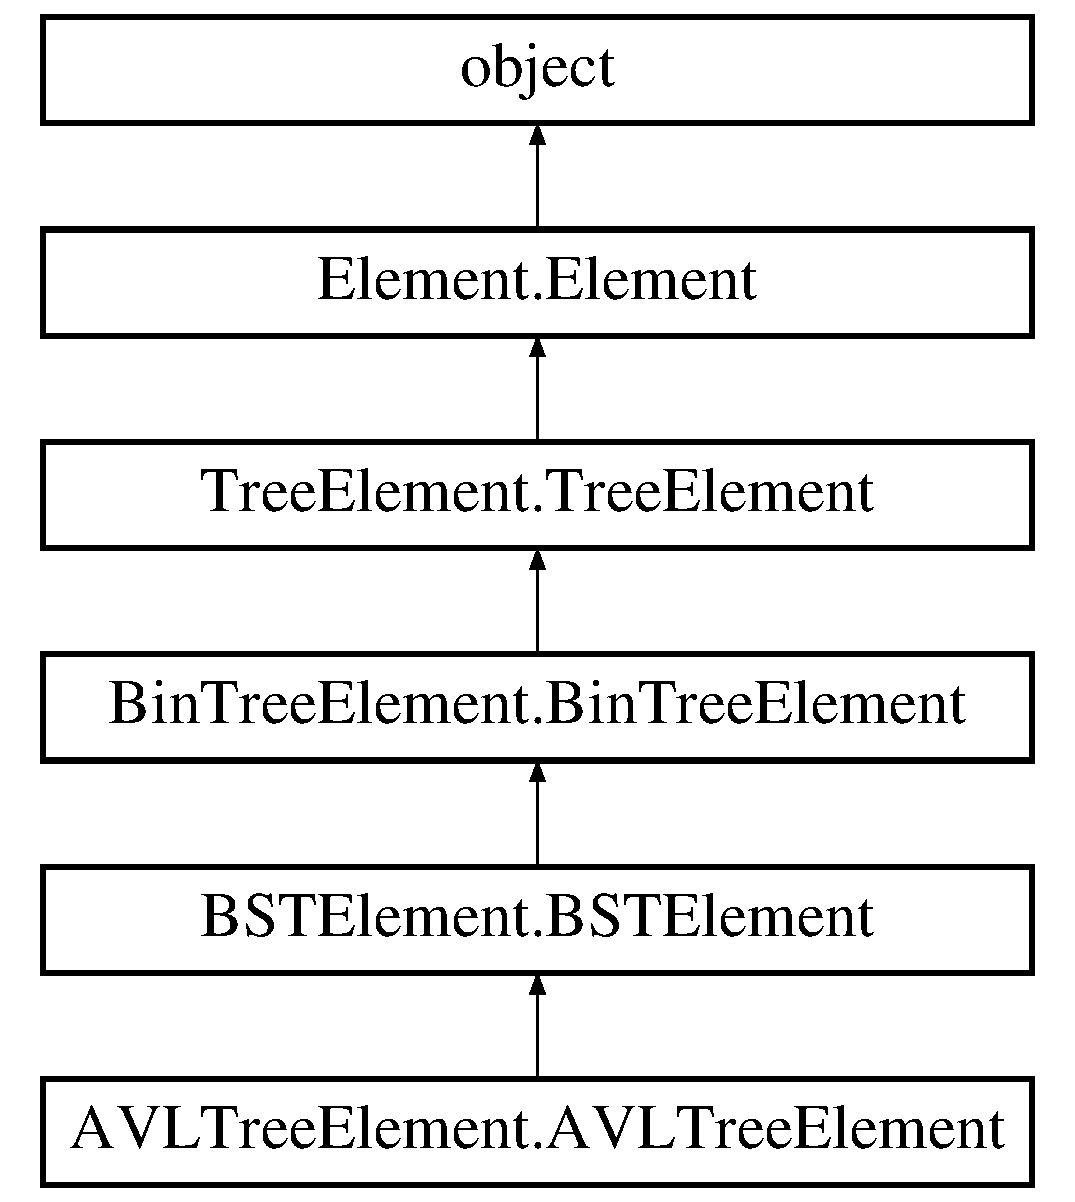
\includegraphics[height=6.000000cm]{class_b_s_t_element_1_1_b_s_t_element}
\end{center}
\end{figure}
\subsection*{Public Member Functions}
\begin{DoxyCompactItemize}
\item 
def \hyperlink{class_b_s_t_element_1_1_b_s_t_element_a0a287cbb68ee9a5fbdbba5c808c1fcd6}{\+\_\+\+\_\+init\+\_\+\+\_\+}
\item 
def \hyperlink{class_b_s_t_element_1_1_b_s_t_element_ad372cf1cbc29e996427ab2162a9dbcaf}{get\+\_\+data\+\_\+structure\+\_\+type} (self)
\item 
def \hyperlink{class_b_s_t_element_1_1_b_s_t_element_aa67ecd77bfb90e10dfa634c114056a56}{get\+\_\+key} (self)
\item 
def \hyperlink{class_b_s_t_element_1_1_b_s_t_element_a5db294d56393f73346b4e55816300c14}{set\+\_\+key} (self, \hyperlink{class_b_s_t_element_1_1_b_s_t_element_aa6ae6b6dad6bf59b65a55ec3f94abcfb}{key})
\item 
def \hyperlink{class_b_s_t_element_1_1_b_s_t_element_aa892f1b8dc467de6bba5ebed365c3bd5}{get\+\_\+left} (self)
\item 
def \hyperlink{class_b_s_t_element_1_1_b_s_t_element_a8a67132b355933640bf13efd74741468}{get\+\_\+right} (self)
\end{DoxyCompactItemize}
\subsection*{Public Attributes}
\begin{DoxyCompactItemize}
\item 
\hyperlink{class_b_s_t_element_1_1_b_s_t_element_a735558f94dd610c6f8ce54ecd3446ed1}{key}
\end{DoxyCompactItemize}
\subsection*{Static Public Attributes}
\begin{DoxyCompactItemize}
\item 
tuple \hyperlink{class_b_s_t_element_1_1_b_s_t_element_aa6ae6b6dad6bf59b65a55ec3f94abcfb}{key} = object()
\end{DoxyCompactItemize}


\subsection{Constructor \& Destructor Documentation}
\hypertarget{class_b_s_t_element_1_1_b_s_t_element_a0a287cbb68ee9a5fbdbba5c808c1fcd6}{}\index{B\+S\+T\+Element\+::\+B\+S\+T\+Element@{B\+S\+T\+Element\+::\+B\+S\+T\+Element}!\+\_\+\+\_\+init\+\_\+\+\_\+@{\+\_\+\+\_\+init\+\_\+\+\_\+}}
\index{\+\_\+\+\_\+init\+\_\+\+\_\+@{\+\_\+\+\_\+init\+\_\+\+\_\+}!B\+S\+T\+Element\+::\+B\+S\+T\+Element@{B\+S\+T\+Element\+::\+B\+S\+T\+Element}}
\subsubsection[{\+\_\+\+\_\+init\+\_\+\+\_\+}]{\setlength{\rightskip}{0pt plus 5cm}def B\+S\+T\+Element.\+B\+S\+T\+Element.\+\_\+\+\_\+init\+\_\+\+\_\+ (
\begin{DoxyParamCaption}
\item[{}]{self, }
\item[{}]{key = {\ttfamily None}, }
\item[{}]{e = {\ttfamily None}, }
\item[{}]{left = {\ttfamily None}, }
\item[{}]{right = {\ttfamily None}, }
\item[{}]{label = {\ttfamily None}}
\end{DoxyParamCaption}
)}\label{class_b_s_t_element_1_1_b_s_t_element_a0a287cbb68ee9a5fbdbba5c808c1fcd6}


\subsection{Member Function Documentation}
\hypertarget{class_b_s_t_element_1_1_b_s_t_element_ad372cf1cbc29e996427ab2162a9dbcaf}{}\index{B\+S\+T\+Element\+::\+B\+S\+T\+Element@{B\+S\+T\+Element\+::\+B\+S\+T\+Element}!get\+\_\+data\+\_\+structure\+\_\+type@{get\+\_\+data\+\_\+structure\+\_\+type}}
\index{get\+\_\+data\+\_\+structure\+\_\+type@{get\+\_\+data\+\_\+structure\+\_\+type}!B\+S\+T\+Element\+::\+B\+S\+T\+Element@{B\+S\+T\+Element\+::\+B\+S\+T\+Element}}
\subsubsection[{get\+\_\+data\+\_\+structure\+\_\+type(self)}]{\setlength{\rightskip}{0pt plus 5cm}def B\+S\+T\+Element.\+B\+S\+T\+Element.\+get\+\_\+data\+\_\+structure\+\_\+type (
\begin{DoxyParamCaption}
\item[{}]{self}
\end{DoxyParamCaption}
)}\label{class_b_s_t_element_1_1_b_s_t_element_ad372cf1cbc29e996427ab2162a9dbcaf}
\hypertarget{class_b_s_t_element_1_1_b_s_t_element_aa67ecd77bfb90e10dfa634c114056a56}{}\index{B\+S\+T\+Element\+::\+B\+S\+T\+Element@{B\+S\+T\+Element\+::\+B\+S\+T\+Element}!get\+\_\+key@{get\+\_\+key}}
\index{get\+\_\+key@{get\+\_\+key}!B\+S\+T\+Element\+::\+B\+S\+T\+Element@{B\+S\+T\+Element\+::\+B\+S\+T\+Element}}
\subsubsection[{get\+\_\+key(self)}]{\setlength{\rightskip}{0pt plus 5cm}def B\+S\+T\+Element.\+B\+S\+T\+Element.\+get\+\_\+key (
\begin{DoxyParamCaption}
\item[{}]{self}
\end{DoxyParamCaption}
)}\label{class_b_s_t_element_1_1_b_s_t_element_aa67ecd77bfb90e10dfa634c114056a56}
\hypertarget{class_b_s_t_element_1_1_b_s_t_element_aa892f1b8dc467de6bba5ebed365c3bd5}{}\index{B\+S\+T\+Element\+::\+B\+S\+T\+Element@{B\+S\+T\+Element\+::\+B\+S\+T\+Element}!get\+\_\+left@{get\+\_\+left}}
\index{get\+\_\+left@{get\+\_\+left}!B\+S\+T\+Element\+::\+B\+S\+T\+Element@{B\+S\+T\+Element\+::\+B\+S\+T\+Element}}
\subsubsection[{get\+\_\+left(self)}]{\setlength{\rightskip}{0pt plus 5cm}def B\+S\+T\+Element.\+B\+S\+T\+Element.\+get\+\_\+left (
\begin{DoxyParamCaption}
\item[{}]{self}
\end{DoxyParamCaption}
)}\label{class_b_s_t_element_1_1_b_s_t_element_aa892f1b8dc467de6bba5ebed365c3bd5}
\hypertarget{class_b_s_t_element_1_1_b_s_t_element_a8a67132b355933640bf13efd74741468}{}\index{B\+S\+T\+Element\+::\+B\+S\+T\+Element@{B\+S\+T\+Element\+::\+B\+S\+T\+Element}!get\+\_\+right@{get\+\_\+right}}
\index{get\+\_\+right@{get\+\_\+right}!B\+S\+T\+Element\+::\+B\+S\+T\+Element@{B\+S\+T\+Element\+::\+B\+S\+T\+Element}}
\subsubsection[{get\+\_\+right(self)}]{\setlength{\rightskip}{0pt plus 5cm}def B\+S\+T\+Element.\+B\+S\+T\+Element.\+get\+\_\+right (
\begin{DoxyParamCaption}
\item[{}]{self}
\end{DoxyParamCaption}
)}\label{class_b_s_t_element_1_1_b_s_t_element_a8a67132b355933640bf13efd74741468}
\hypertarget{class_b_s_t_element_1_1_b_s_t_element_a5db294d56393f73346b4e55816300c14}{}\index{B\+S\+T\+Element\+::\+B\+S\+T\+Element@{B\+S\+T\+Element\+::\+B\+S\+T\+Element}!set\+\_\+key@{set\+\_\+key}}
\index{set\+\_\+key@{set\+\_\+key}!B\+S\+T\+Element\+::\+B\+S\+T\+Element@{B\+S\+T\+Element\+::\+B\+S\+T\+Element}}
\subsubsection[{set\+\_\+key(self, key)}]{\setlength{\rightskip}{0pt plus 5cm}def B\+S\+T\+Element.\+B\+S\+T\+Element.\+set\+\_\+key (
\begin{DoxyParamCaption}
\item[{}]{self, }
\item[{}]{key}
\end{DoxyParamCaption}
)}\label{class_b_s_t_element_1_1_b_s_t_element_a5db294d56393f73346b4e55816300c14}


\subsection{Member Data Documentation}
\hypertarget{class_b_s_t_element_1_1_b_s_t_element_aa6ae6b6dad6bf59b65a55ec3f94abcfb}{}\index{B\+S\+T\+Element\+::\+B\+S\+T\+Element@{B\+S\+T\+Element\+::\+B\+S\+T\+Element}!key@{key}}
\index{key@{key}!B\+S\+T\+Element\+::\+B\+S\+T\+Element@{B\+S\+T\+Element\+::\+B\+S\+T\+Element}}
\subsubsection[{key}]{\setlength{\rightskip}{0pt plus 5cm}tuple B\+S\+T\+Element.\+B\+S\+T\+Element.\+key = object()\hspace{0.3cm}{\ttfamily [static]}}\label{class_b_s_t_element_1_1_b_s_t_element_aa6ae6b6dad6bf59b65a55ec3f94abcfb}
\hypertarget{class_b_s_t_element_1_1_b_s_t_element_a735558f94dd610c6f8ce54ecd3446ed1}{}\index{B\+S\+T\+Element\+::\+B\+S\+T\+Element@{B\+S\+T\+Element\+::\+B\+S\+T\+Element}!key@{key}}
\index{key@{key}!B\+S\+T\+Element\+::\+B\+S\+T\+Element@{B\+S\+T\+Element\+::\+B\+S\+T\+Element}}
\subsubsection[{key}]{\setlength{\rightskip}{0pt plus 5cm}B\+S\+T\+Element.\+B\+S\+T\+Element.\+key}\label{class_b_s_t_element_1_1_b_s_t_element_a735558f94dd610c6f8ce54ecd3446ed1}


The documentation for this class was generated from the following file\+:\begin{DoxyCompactItemize}
\item 
/\+Users/krs/gr/bridges/bridges17/python/src/\hyperlink{_b_s_t_element_8py}{B\+S\+T\+Element.\+py}\end{DoxyCompactItemize}

\hypertarget{class_cancer_incidence_1_1_cancer_incidence}{}\section{Cancer\+Incidence.\+Cancer\+Incidence Class Reference}
\label{class_cancer_incidence_1_1_cancer_incidence}\index{Cancer\+Incidence.\+Cancer\+Incidence@{Cancer\+Incidence.\+Cancer\+Incidence}}
\subsection*{Public Member Functions}
\begin{DoxyCompactItemize}
\item 
def \hyperlink{class_cancer_incidence_1_1_cancer_incidence_ad426f06ec5738a32bf25a24bad0d5d48}{\+\_\+\+\_\+init\+\_\+\+\_\+} (self)
\item 
def \hyperlink{class_cancer_incidence_1_1_cancer_incidence_a4b774ff7c72de4d71cec56899a9f7862}{get\+Age\+Adjusted\+Rate} (self)
\item 
def \hyperlink{class_cancer_incidence_1_1_cancer_incidence_ac384d7a65a9f6c4907b95a28994ae6a8}{set\+Age\+Adjusted\+Rate} (self, arr)
\item 
def \hyperlink{class_cancer_incidence_1_1_cancer_incidence_a6b7a1de864b12d25e86a70906ef24bbd}{get\+Age\+Adjusted\+C\+I\+\_\+\+Lower} (self)
\item 
def \hyperlink{class_cancer_incidence_1_1_cancer_incidence_a9dff100ca9a7f8547dca88b0d8f383b4}{set\+Age\+Adjusted\+C\+I\+\_\+\+Lower} (self, ci\+\_\+l)
\item 
def \hyperlink{class_cancer_incidence_1_1_cancer_incidence_aa6bd6e0a0f1f9106c7e094bce310c5d4}{get\+Age\+Adjusted\+C\+I\+\_\+\+Upper} (self)
\item 
def \hyperlink{class_cancer_incidence_1_1_cancer_incidence_aab0e4d5aa0b3f7850e30b2ccb9e433fa}{set\+Age\+Adjusted\+C\+I\+\_\+\+Upper} (self, ci\+\_\+u)
\item 
def \hyperlink{class_cancer_incidence_1_1_cancer_incidence_a346895f923cb82648d5add0c5fd4e1c6}{get\+Crude\+Rate} (self)
\item 
def \hyperlink{class_cancer_incidence_1_1_cancer_incidence_abf45feac9bd6017eb8326d51d7e3fec6}{set\+Crude\+Rate} (self, cr)
\item 
def \hyperlink{class_cancer_incidence_1_1_cancer_incidence_a5788d3e3a92f16dfea080a4ee9f9874e}{get\+Crude\+Rate\+\_\+\+C\+I\+\_\+\+Lower} (self)
\item 
def \hyperlink{class_cancer_incidence_1_1_cancer_incidence_af20a3b98541017472d2be3f784460d46}{set\+Crude\+Rate\+\_\+\+C\+I\+\_\+lower} (self, cr\+\_\+l)
\item 
def \hyperlink{class_cancer_incidence_1_1_cancer_incidence_ab1fe4d09048943cca049a54ab78555ff}{get\+Crude\+Rate\+\_\+\+C\+I\+\_\+\+Upper} (self)
\item 
def \hyperlink{class_cancer_incidence_1_1_cancer_incidence_a73a869d9fe2fc5204955b209e32cc95b}{set\+Crude\+Rate\+\_\+\+C\+I\+\_\+\+Upper} (self, cr\+\_\+l)
\item 
def \hyperlink{class_cancer_incidence_1_1_cancer_incidence_a2b4025524c97ab72835a0b768000b0ad}{get\+Year} (self)
\item 
def \hyperlink{class_cancer_incidence_1_1_cancer_incidence_a4f9224921e9b4db7f088a6106f8a8f7e}{set\+Year} (self, \hyperlink{class_cancer_incidence_1_1_cancer_incidence_ad3ebc04a77307ff150f2d6f0f95b3de7}{year})
\item 
def \hyperlink{class_cancer_incidence_1_1_cancer_incidence_adf68d56c535f187e9268fcab4a871c2f}{get\+Gender} (self)
\item 
def \hyperlink{class_cancer_incidence_1_1_cancer_incidence_ab8332b3081a15fedaa892dd1735e6260}{set\+Gender} (self, \hyperlink{class_cancer_incidence_1_1_cancer_incidence_ad8f6e9c194bed1ced8a6ce0f8e1678f0}{gender})
\item 
def \hyperlink{class_cancer_incidence_1_1_cancer_incidence_a83c1c0dc576c66fa450f2f1346760715}{get\+Race} (self)
\item 
def \hyperlink{class_cancer_incidence_1_1_cancer_incidence_ab52a637061d5530a27cc5c3e5af251c1}{set\+Race} (self, \hyperlink{class_cancer_incidence_1_1_cancer_incidence_aabf2d41cf0000d41fb135b2801b35334}{race})
\item 
def \hyperlink{class_cancer_incidence_1_1_cancer_incidence_ae6237eeb2c52e3593a230ba3947d39e6}{get\+Event\+Type} (self)
\item 
def \hyperlink{class_cancer_incidence_1_1_cancer_incidence_a10236a59ed482edb0febff96cedeb686}{set\+Event\+Type} (self, et)
\item 
def \hyperlink{class_cancer_incidence_1_1_cancer_incidence_a20e27155f5454c7877cb20a99bfc8770}{get\+Population} (self)
\item 
def \hyperlink{class_cancer_incidence_1_1_cancer_incidence_aac5268c0c943e895e423dc973e5c365e}{set\+Population} (self, pop)
\item 
def \hyperlink{class_cancer_incidence_1_1_cancer_incidence_ac4b3c0aabba84934bea6cc8bad7738f3}{get\+Affected\+Area} (self)
\item 
def \hyperlink{class_cancer_incidence_1_1_cancer_incidence_a5b493f09514dc25126b3692dfb4f72c6}{set\+Affected\+Area} (self, area)
\item 
def \hyperlink{class_cancer_incidence_1_1_cancer_incidence_a6ccdad0af30eead93ffe3e249310ae49}{get\+Count} (self)
\item 
def \hyperlink{class_cancer_incidence_1_1_cancer_incidence_a425ab75f9d216721d767fad7af0fc196}{set\+Count} (self, \hyperlink{class_cancer_incidence_1_1_cancer_incidence_a7627584cd6a537797741c291833ca0c6}{count})
\item 
def \hyperlink{class_cancer_incidence_1_1_cancer_incidence_a2ce5e8362ab8d0948230775cca9161b2}{get\+Location\+X} (self)
\item 
def \hyperlink{class_cancer_incidence_1_1_cancer_incidence_a8cfea368d1cda9b94fcac03f116dfe4e}{set\+Location\+X} (self, x)
\item 
def \hyperlink{class_cancer_incidence_1_1_cancer_incidence_a3e5fe2583e2eafd1c7543114f68f3dcb}{get\+Location\+Y} (self)
\item 
def \hyperlink{class_cancer_incidence_1_1_cancer_incidence_ad8585a3252d4cbf30959daa47d731179}{set\+Location\+Y} (self, y)
\end{DoxyCompactItemize}
\subsection*{Public Attributes}
\begin{DoxyCompactItemize}
\item 
\hyperlink{class_cancer_incidence_1_1_cancer_incidence_aab4355a92c91c9adde2f38e62c8f499d}{loc}
\item 
\hyperlink{class_cancer_incidence_1_1_cancer_incidence_ad3ebc04a77307ff150f2d6f0f95b3de7}{year}
\item 
\hyperlink{class_cancer_incidence_1_1_cancer_incidence_a7627584cd6a537797741c291833ca0c6}{count}
\item 
\hyperlink{class_cancer_incidence_1_1_cancer_incidence_ac89ae8d4a5a136f71dc339d4af256904}{population}
\item 
\hyperlink{class_cancer_incidence_1_1_cancer_incidence_ad8f6e9c194bed1ced8a6ce0f8e1678f0}{gender}
\item 
\hyperlink{class_cancer_incidence_1_1_cancer_incidence_aabf2d41cf0000d41fb135b2801b35334}{race}
\item 
\hyperlink{class_cancer_incidence_1_1_cancer_incidence_a84cfbb0f8518f5b63ab09d61cf020984}{event\+\_\+type}
\item 
\hyperlink{class_cancer_incidence_1_1_cancer_incidence_aed83029c9ab4fdda4ecea2c4eda29c63}{affected\+\_\+area}
\item 
\hyperlink{class_cancer_incidence_1_1_cancer_incidence_ac799c09cc336e00b0723fe9d0ecde5ab}{age\+Adjusted\+Rate}
\item 
\hyperlink{class_cancer_incidence_1_1_cancer_incidence_a55e91b4b3cf8fce6fd37a7c0e5ca1a52}{crude\+Rate}
\item 
\hyperlink{class_cancer_incidence_1_1_cancer_incidence_af7848cd32d6e2c45bdd12500aed2c4f3}{age\+Adjusted\+Rateci}
\item 
\hyperlink{class_cancer_incidence_1_1_cancer_incidence_aece0ef64d99a5dbbb4b9ac4592e8fddc}{crude\+Rateci}
\end{DoxyCompactItemize}


\subsection{Constructor \& Destructor Documentation}
\hypertarget{class_cancer_incidence_1_1_cancer_incidence_ad426f06ec5738a32bf25a24bad0d5d48}{}\index{Cancer\+Incidence\+::\+Cancer\+Incidence@{Cancer\+Incidence\+::\+Cancer\+Incidence}!\+\_\+\+\_\+init\+\_\+\+\_\+@{\+\_\+\+\_\+init\+\_\+\+\_\+}}
\index{\+\_\+\+\_\+init\+\_\+\+\_\+@{\+\_\+\+\_\+init\+\_\+\+\_\+}!Cancer\+Incidence\+::\+Cancer\+Incidence@{Cancer\+Incidence\+::\+Cancer\+Incidence}}
\subsubsection[{\+\_\+\+\_\+init\+\_\+\+\_\+(self)}]{\setlength{\rightskip}{0pt plus 5cm}def Cancer\+Incidence.\+Cancer\+Incidence.\+\_\+\+\_\+init\+\_\+\+\_\+ (
\begin{DoxyParamCaption}
\item[{}]{self}
\end{DoxyParamCaption}
)}\label{class_cancer_incidence_1_1_cancer_incidence_ad426f06ec5738a32bf25a24bad0d5d48}


\subsection{Member Function Documentation}
\hypertarget{class_cancer_incidence_1_1_cancer_incidence_ac4b3c0aabba84934bea6cc8bad7738f3}{}\index{Cancer\+Incidence\+::\+Cancer\+Incidence@{Cancer\+Incidence\+::\+Cancer\+Incidence}!get\+Affected\+Area@{get\+Affected\+Area}}
\index{get\+Affected\+Area@{get\+Affected\+Area}!Cancer\+Incidence\+::\+Cancer\+Incidence@{Cancer\+Incidence\+::\+Cancer\+Incidence}}
\subsubsection[{get\+Affected\+Area(self)}]{\setlength{\rightskip}{0pt plus 5cm}def Cancer\+Incidence.\+Cancer\+Incidence.\+get\+Affected\+Area (
\begin{DoxyParamCaption}
\item[{}]{self}
\end{DoxyParamCaption}
)}\label{class_cancer_incidence_1_1_cancer_incidence_ac4b3c0aabba84934bea6cc8bad7738f3}
\hypertarget{class_cancer_incidence_1_1_cancer_incidence_a6b7a1de864b12d25e86a70906ef24bbd}{}\index{Cancer\+Incidence\+::\+Cancer\+Incidence@{Cancer\+Incidence\+::\+Cancer\+Incidence}!get\+Age\+Adjusted\+C\+I\+\_\+\+Lower@{get\+Age\+Adjusted\+C\+I\+\_\+\+Lower}}
\index{get\+Age\+Adjusted\+C\+I\+\_\+\+Lower@{get\+Age\+Adjusted\+C\+I\+\_\+\+Lower}!Cancer\+Incidence\+::\+Cancer\+Incidence@{Cancer\+Incidence\+::\+Cancer\+Incidence}}
\subsubsection[{get\+Age\+Adjusted\+C\+I\+\_\+\+Lower(self)}]{\setlength{\rightskip}{0pt plus 5cm}def Cancer\+Incidence.\+Cancer\+Incidence.\+get\+Age\+Adjusted\+C\+I\+\_\+\+Lower (
\begin{DoxyParamCaption}
\item[{}]{self}
\end{DoxyParamCaption}
)}\label{class_cancer_incidence_1_1_cancer_incidence_a6b7a1de864b12d25e86a70906ef24bbd}
\hypertarget{class_cancer_incidence_1_1_cancer_incidence_aa6bd6e0a0f1f9106c7e094bce310c5d4}{}\index{Cancer\+Incidence\+::\+Cancer\+Incidence@{Cancer\+Incidence\+::\+Cancer\+Incidence}!get\+Age\+Adjusted\+C\+I\+\_\+\+Upper@{get\+Age\+Adjusted\+C\+I\+\_\+\+Upper}}
\index{get\+Age\+Adjusted\+C\+I\+\_\+\+Upper@{get\+Age\+Adjusted\+C\+I\+\_\+\+Upper}!Cancer\+Incidence\+::\+Cancer\+Incidence@{Cancer\+Incidence\+::\+Cancer\+Incidence}}
\subsubsection[{get\+Age\+Adjusted\+C\+I\+\_\+\+Upper(self)}]{\setlength{\rightskip}{0pt plus 5cm}def Cancer\+Incidence.\+Cancer\+Incidence.\+get\+Age\+Adjusted\+C\+I\+\_\+\+Upper (
\begin{DoxyParamCaption}
\item[{}]{self}
\end{DoxyParamCaption}
)}\label{class_cancer_incidence_1_1_cancer_incidence_aa6bd6e0a0f1f9106c7e094bce310c5d4}
\hypertarget{class_cancer_incidence_1_1_cancer_incidence_a4b774ff7c72de4d71cec56899a9f7862}{}\index{Cancer\+Incidence\+::\+Cancer\+Incidence@{Cancer\+Incidence\+::\+Cancer\+Incidence}!get\+Age\+Adjusted\+Rate@{get\+Age\+Adjusted\+Rate}}
\index{get\+Age\+Adjusted\+Rate@{get\+Age\+Adjusted\+Rate}!Cancer\+Incidence\+::\+Cancer\+Incidence@{Cancer\+Incidence\+::\+Cancer\+Incidence}}
\subsubsection[{get\+Age\+Adjusted\+Rate(self)}]{\setlength{\rightskip}{0pt plus 5cm}def Cancer\+Incidence.\+Cancer\+Incidence.\+get\+Age\+Adjusted\+Rate (
\begin{DoxyParamCaption}
\item[{}]{self}
\end{DoxyParamCaption}
)}\label{class_cancer_incidence_1_1_cancer_incidence_a4b774ff7c72de4d71cec56899a9f7862}
\hypertarget{class_cancer_incidence_1_1_cancer_incidence_a6ccdad0af30eead93ffe3e249310ae49}{}\index{Cancer\+Incidence\+::\+Cancer\+Incidence@{Cancer\+Incidence\+::\+Cancer\+Incidence}!get\+Count@{get\+Count}}
\index{get\+Count@{get\+Count}!Cancer\+Incidence\+::\+Cancer\+Incidence@{Cancer\+Incidence\+::\+Cancer\+Incidence}}
\subsubsection[{get\+Count(self)}]{\setlength{\rightskip}{0pt plus 5cm}def Cancer\+Incidence.\+Cancer\+Incidence.\+get\+Count (
\begin{DoxyParamCaption}
\item[{}]{self}
\end{DoxyParamCaption}
)}\label{class_cancer_incidence_1_1_cancer_incidence_a6ccdad0af30eead93ffe3e249310ae49}
\hypertarget{class_cancer_incidence_1_1_cancer_incidence_a346895f923cb82648d5add0c5fd4e1c6}{}\index{Cancer\+Incidence\+::\+Cancer\+Incidence@{Cancer\+Incidence\+::\+Cancer\+Incidence}!get\+Crude\+Rate@{get\+Crude\+Rate}}
\index{get\+Crude\+Rate@{get\+Crude\+Rate}!Cancer\+Incidence\+::\+Cancer\+Incidence@{Cancer\+Incidence\+::\+Cancer\+Incidence}}
\subsubsection[{get\+Crude\+Rate(self)}]{\setlength{\rightskip}{0pt plus 5cm}def Cancer\+Incidence.\+Cancer\+Incidence.\+get\+Crude\+Rate (
\begin{DoxyParamCaption}
\item[{}]{self}
\end{DoxyParamCaption}
)}\label{class_cancer_incidence_1_1_cancer_incidence_a346895f923cb82648d5add0c5fd4e1c6}
\hypertarget{class_cancer_incidence_1_1_cancer_incidence_a5788d3e3a92f16dfea080a4ee9f9874e}{}\index{Cancer\+Incidence\+::\+Cancer\+Incidence@{Cancer\+Incidence\+::\+Cancer\+Incidence}!get\+Crude\+Rate\+\_\+\+C\+I\+\_\+\+Lower@{get\+Crude\+Rate\+\_\+\+C\+I\+\_\+\+Lower}}
\index{get\+Crude\+Rate\+\_\+\+C\+I\+\_\+\+Lower@{get\+Crude\+Rate\+\_\+\+C\+I\+\_\+\+Lower}!Cancer\+Incidence\+::\+Cancer\+Incidence@{Cancer\+Incidence\+::\+Cancer\+Incidence}}
\subsubsection[{get\+Crude\+Rate\+\_\+\+C\+I\+\_\+\+Lower(self)}]{\setlength{\rightskip}{0pt plus 5cm}def Cancer\+Incidence.\+Cancer\+Incidence.\+get\+Crude\+Rate\+\_\+\+C\+I\+\_\+\+Lower (
\begin{DoxyParamCaption}
\item[{}]{self}
\end{DoxyParamCaption}
)}\label{class_cancer_incidence_1_1_cancer_incidence_a5788d3e3a92f16dfea080a4ee9f9874e}
\hypertarget{class_cancer_incidence_1_1_cancer_incidence_ab1fe4d09048943cca049a54ab78555ff}{}\index{Cancer\+Incidence\+::\+Cancer\+Incidence@{Cancer\+Incidence\+::\+Cancer\+Incidence}!get\+Crude\+Rate\+\_\+\+C\+I\+\_\+\+Upper@{get\+Crude\+Rate\+\_\+\+C\+I\+\_\+\+Upper}}
\index{get\+Crude\+Rate\+\_\+\+C\+I\+\_\+\+Upper@{get\+Crude\+Rate\+\_\+\+C\+I\+\_\+\+Upper}!Cancer\+Incidence\+::\+Cancer\+Incidence@{Cancer\+Incidence\+::\+Cancer\+Incidence}}
\subsubsection[{get\+Crude\+Rate\+\_\+\+C\+I\+\_\+\+Upper(self)}]{\setlength{\rightskip}{0pt plus 5cm}def Cancer\+Incidence.\+Cancer\+Incidence.\+get\+Crude\+Rate\+\_\+\+C\+I\+\_\+\+Upper (
\begin{DoxyParamCaption}
\item[{}]{self}
\end{DoxyParamCaption}
)}\label{class_cancer_incidence_1_1_cancer_incidence_ab1fe4d09048943cca049a54ab78555ff}
\hypertarget{class_cancer_incidence_1_1_cancer_incidence_ae6237eeb2c52e3593a230ba3947d39e6}{}\index{Cancer\+Incidence\+::\+Cancer\+Incidence@{Cancer\+Incidence\+::\+Cancer\+Incidence}!get\+Event\+Type@{get\+Event\+Type}}
\index{get\+Event\+Type@{get\+Event\+Type}!Cancer\+Incidence\+::\+Cancer\+Incidence@{Cancer\+Incidence\+::\+Cancer\+Incidence}}
\subsubsection[{get\+Event\+Type(self)}]{\setlength{\rightskip}{0pt plus 5cm}def Cancer\+Incidence.\+Cancer\+Incidence.\+get\+Event\+Type (
\begin{DoxyParamCaption}
\item[{}]{self}
\end{DoxyParamCaption}
)}\label{class_cancer_incidence_1_1_cancer_incidence_ae6237eeb2c52e3593a230ba3947d39e6}
\hypertarget{class_cancer_incidence_1_1_cancer_incidence_adf68d56c535f187e9268fcab4a871c2f}{}\index{Cancer\+Incidence\+::\+Cancer\+Incidence@{Cancer\+Incidence\+::\+Cancer\+Incidence}!get\+Gender@{get\+Gender}}
\index{get\+Gender@{get\+Gender}!Cancer\+Incidence\+::\+Cancer\+Incidence@{Cancer\+Incidence\+::\+Cancer\+Incidence}}
\subsubsection[{get\+Gender(self)}]{\setlength{\rightskip}{0pt plus 5cm}def Cancer\+Incidence.\+Cancer\+Incidence.\+get\+Gender (
\begin{DoxyParamCaption}
\item[{}]{self}
\end{DoxyParamCaption}
)}\label{class_cancer_incidence_1_1_cancer_incidence_adf68d56c535f187e9268fcab4a871c2f}
\hypertarget{class_cancer_incidence_1_1_cancer_incidence_a2ce5e8362ab8d0948230775cca9161b2}{}\index{Cancer\+Incidence\+::\+Cancer\+Incidence@{Cancer\+Incidence\+::\+Cancer\+Incidence}!get\+Location\+X@{get\+Location\+X}}
\index{get\+Location\+X@{get\+Location\+X}!Cancer\+Incidence\+::\+Cancer\+Incidence@{Cancer\+Incidence\+::\+Cancer\+Incidence}}
\subsubsection[{get\+Location\+X(self)}]{\setlength{\rightskip}{0pt plus 5cm}def Cancer\+Incidence.\+Cancer\+Incidence.\+get\+Location\+X (
\begin{DoxyParamCaption}
\item[{}]{self}
\end{DoxyParamCaption}
)}\label{class_cancer_incidence_1_1_cancer_incidence_a2ce5e8362ab8d0948230775cca9161b2}
\hypertarget{class_cancer_incidence_1_1_cancer_incidence_a3e5fe2583e2eafd1c7543114f68f3dcb}{}\index{Cancer\+Incidence\+::\+Cancer\+Incidence@{Cancer\+Incidence\+::\+Cancer\+Incidence}!get\+Location\+Y@{get\+Location\+Y}}
\index{get\+Location\+Y@{get\+Location\+Y}!Cancer\+Incidence\+::\+Cancer\+Incidence@{Cancer\+Incidence\+::\+Cancer\+Incidence}}
\subsubsection[{get\+Location\+Y(self)}]{\setlength{\rightskip}{0pt plus 5cm}def Cancer\+Incidence.\+Cancer\+Incidence.\+get\+Location\+Y (
\begin{DoxyParamCaption}
\item[{}]{self}
\end{DoxyParamCaption}
)}\label{class_cancer_incidence_1_1_cancer_incidence_a3e5fe2583e2eafd1c7543114f68f3dcb}
\hypertarget{class_cancer_incidence_1_1_cancer_incidence_a20e27155f5454c7877cb20a99bfc8770}{}\index{Cancer\+Incidence\+::\+Cancer\+Incidence@{Cancer\+Incidence\+::\+Cancer\+Incidence}!get\+Population@{get\+Population}}
\index{get\+Population@{get\+Population}!Cancer\+Incidence\+::\+Cancer\+Incidence@{Cancer\+Incidence\+::\+Cancer\+Incidence}}
\subsubsection[{get\+Population(self)}]{\setlength{\rightskip}{0pt plus 5cm}def Cancer\+Incidence.\+Cancer\+Incidence.\+get\+Population (
\begin{DoxyParamCaption}
\item[{}]{self}
\end{DoxyParamCaption}
)}\label{class_cancer_incidence_1_1_cancer_incidence_a20e27155f5454c7877cb20a99bfc8770}
\hypertarget{class_cancer_incidence_1_1_cancer_incidence_a83c1c0dc576c66fa450f2f1346760715}{}\index{Cancer\+Incidence\+::\+Cancer\+Incidence@{Cancer\+Incidence\+::\+Cancer\+Incidence}!get\+Race@{get\+Race}}
\index{get\+Race@{get\+Race}!Cancer\+Incidence\+::\+Cancer\+Incidence@{Cancer\+Incidence\+::\+Cancer\+Incidence}}
\subsubsection[{get\+Race(self)}]{\setlength{\rightskip}{0pt plus 5cm}def Cancer\+Incidence.\+Cancer\+Incidence.\+get\+Race (
\begin{DoxyParamCaption}
\item[{}]{self}
\end{DoxyParamCaption}
)}\label{class_cancer_incidence_1_1_cancer_incidence_a83c1c0dc576c66fa450f2f1346760715}
\hypertarget{class_cancer_incidence_1_1_cancer_incidence_a2b4025524c97ab72835a0b768000b0ad}{}\index{Cancer\+Incidence\+::\+Cancer\+Incidence@{Cancer\+Incidence\+::\+Cancer\+Incidence}!get\+Year@{get\+Year}}
\index{get\+Year@{get\+Year}!Cancer\+Incidence\+::\+Cancer\+Incidence@{Cancer\+Incidence\+::\+Cancer\+Incidence}}
\subsubsection[{get\+Year(self)}]{\setlength{\rightskip}{0pt plus 5cm}def Cancer\+Incidence.\+Cancer\+Incidence.\+get\+Year (
\begin{DoxyParamCaption}
\item[{}]{self}
\end{DoxyParamCaption}
)}\label{class_cancer_incidence_1_1_cancer_incidence_a2b4025524c97ab72835a0b768000b0ad}
\hypertarget{class_cancer_incidence_1_1_cancer_incidence_a5b493f09514dc25126b3692dfb4f72c6}{}\index{Cancer\+Incidence\+::\+Cancer\+Incidence@{Cancer\+Incidence\+::\+Cancer\+Incidence}!set\+Affected\+Area@{set\+Affected\+Area}}
\index{set\+Affected\+Area@{set\+Affected\+Area}!Cancer\+Incidence\+::\+Cancer\+Incidence@{Cancer\+Incidence\+::\+Cancer\+Incidence}}
\subsubsection[{set\+Affected\+Area(self, area)}]{\setlength{\rightskip}{0pt plus 5cm}def Cancer\+Incidence.\+Cancer\+Incidence.\+set\+Affected\+Area (
\begin{DoxyParamCaption}
\item[{}]{self, }
\item[{}]{area}
\end{DoxyParamCaption}
)}\label{class_cancer_incidence_1_1_cancer_incidence_a5b493f09514dc25126b3692dfb4f72c6}
\hypertarget{class_cancer_incidence_1_1_cancer_incidence_a9dff100ca9a7f8547dca88b0d8f383b4}{}\index{Cancer\+Incidence\+::\+Cancer\+Incidence@{Cancer\+Incidence\+::\+Cancer\+Incidence}!set\+Age\+Adjusted\+C\+I\+\_\+\+Lower@{set\+Age\+Adjusted\+C\+I\+\_\+\+Lower}}
\index{set\+Age\+Adjusted\+C\+I\+\_\+\+Lower@{set\+Age\+Adjusted\+C\+I\+\_\+\+Lower}!Cancer\+Incidence\+::\+Cancer\+Incidence@{Cancer\+Incidence\+::\+Cancer\+Incidence}}
\subsubsection[{set\+Age\+Adjusted\+C\+I\+\_\+\+Lower(self, ci\+\_\+l)}]{\setlength{\rightskip}{0pt plus 5cm}def Cancer\+Incidence.\+Cancer\+Incidence.\+set\+Age\+Adjusted\+C\+I\+\_\+\+Lower (
\begin{DoxyParamCaption}
\item[{}]{self, }
\item[{}]{ci\+\_\+l}
\end{DoxyParamCaption}
)}\label{class_cancer_incidence_1_1_cancer_incidence_a9dff100ca9a7f8547dca88b0d8f383b4}
\hypertarget{class_cancer_incidence_1_1_cancer_incidence_aab0e4d5aa0b3f7850e30b2ccb9e433fa}{}\index{Cancer\+Incidence\+::\+Cancer\+Incidence@{Cancer\+Incidence\+::\+Cancer\+Incidence}!set\+Age\+Adjusted\+C\+I\+\_\+\+Upper@{set\+Age\+Adjusted\+C\+I\+\_\+\+Upper}}
\index{set\+Age\+Adjusted\+C\+I\+\_\+\+Upper@{set\+Age\+Adjusted\+C\+I\+\_\+\+Upper}!Cancer\+Incidence\+::\+Cancer\+Incidence@{Cancer\+Incidence\+::\+Cancer\+Incidence}}
\subsubsection[{set\+Age\+Adjusted\+C\+I\+\_\+\+Upper(self, ci\+\_\+u)}]{\setlength{\rightskip}{0pt plus 5cm}def Cancer\+Incidence.\+Cancer\+Incidence.\+set\+Age\+Adjusted\+C\+I\+\_\+\+Upper (
\begin{DoxyParamCaption}
\item[{}]{self, }
\item[{}]{ci\+\_\+u}
\end{DoxyParamCaption}
)}\label{class_cancer_incidence_1_1_cancer_incidence_aab0e4d5aa0b3f7850e30b2ccb9e433fa}
\hypertarget{class_cancer_incidence_1_1_cancer_incidence_ac384d7a65a9f6c4907b95a28994ae6a8}{}\index{Cancer\+Incidence\+::\+Cancer\+Incidence@{Cancer\+Incidence\+::\+Cancer\+Incidence}!set\+Age\+Adjusted\+Rate@{set\+Age\+Adjusted\+Rate}}
\index{set\+Age\+Adjusted\+Rate@{set\+Age\+Adjusted\+Rate}!Cancer\+Incidence\+::\+Cancer\+Incidence@{Cancer\+Incidence\+::\+Cancer\+Incidence}}
\subsubsection[{set\+Age\+Adjusted\+Rate(self, arr)}]{\setlength{\rightskip}{0pt plus 5cm}def Cancer\+Incidence.\+Cancer\+Incidence.\+set\+Age\+Adjusted\+Rate (
\begin{DoxyParamCaption}
\item[{}]{self, }
\item[{}]{arr}
\end{DoxyParamCaption}
)}\label{class_cancer_incidence_1_1_cancer_incidence_ac384d7a65a9f6c4907b95a28994ae6a8}
\hypertarget{class_cancer_incidence_1_1_cancer_incidence_a425ab75f9d216721d767fad7af0fc196}{}\index{Cancer\+Incidence\+::\+Cancer\+Incidence@{Cancer\+Incidence\+::\+Cancer\+Incidence}!set\+Count@{set\+Count}}
\index{set\+Count@{set\+Count}!Cancer\+Incidence\+::\+Cancer\+Incidence@{Cancer\+Incidence\+::\+Cancer\+Incidence}}
\subsubsection[{set\+Count(self, count)}]{\setlength{\rightskip}{0pt plus 5cm}def Cancer\+Incidence.\+Cancer\+Incidence.\+set\+Count (
\begin{DoxyParamCaption}
\item[{}]{self, }
\item[{}]{count}
\end{DoxyParamCaption}
)}\label{class_cancer_incidence_1_1_cancer_incidence_a425ab75f9d216721d767fad7af0fc196}
\hypertarget{class_cancer_incidence_1_1_cancer_incidence_abf45feac9bd6017eb8326d51d7e3fec6}{}\index{Cancer\+Incidence\+::\+Cancer\+Incidence@{Cancer\+Incidence\+::\+Cancer\+Incidence}!set\+Crude\+Rate@{set\+Crude\+Rate}}
\index{set\+Crude\+Rate@{set\+Crude\+Rate}!Cancer\+Incidence\+::\+Cancer\+Incidence@{Cancer\+Incidence\+::\+Cancer\+Incidence}}
\subsubsection[{set\+Crude\+Rate(self, cr)}]{\setlength{\rightskip}{0pt plus 5cm}def Cancer\+Incidence.\+Cancer\+Incidence.\+set\+Crude\+Rate (
\begin{DoxyParamCaption}
\item[{}]{self, }
\item[{}]{cr}
\end{DoxyParamCaption}
)}\label{class_cancer_incidence_1_1_cancer_incidence_abf45feac9bd6017eb8326d51d7e3fec6}
\hypertarget{class_cancer_incidence_1_1_cancer_incidence_af20a3b98541017472d2be3f784460d46}{}\index{Cancer\+Incidence\+::\+Cancer\+Incidence@{Cancer\+Incidence\+::\+Cancer\+Incidence}!set\+Crude\+Rate\+\_\+\+C\+I\+\_\+lower@{set\+Crude\+Rate\+\_\+\+C\+I\+\_\+lower}}
\index{set\+Crude\+Rate\+\_\+\+C\+I\+\_\+lower@{set\+Crude\+Rate\+\_\+\+C\+I\+\_\+lower}!Cancer\+Incidence\+::\+Cancer\+Incidence@{Cancer\+Incidence\+::\+Cancer\+Incidence}}
\subsubsection[{set\+Crude\+Rate\+\_\+\+C\+I\+\_\+lower(self, cr\+\_\+l)}]{\setlength{\rightskip}{0pt plus 5cm}def Cancer\+Incidence.\+Cancer\+Incidence.\+set\+Crude\+Rate\+\_\+\+C\+I\+\_\+lower (
\begin{DoxyParamCaption}
\item[{}]{self, }
\item[{}]{cr\+\_\+l}
\end{DoxyParamCaption}
)}\label{class_cancer_incidence_1_1_cancer_incidence_af20a3b98541017472d2be3f784460d46}
\hypertarget{class_cancer_incidence_1_1_cancer_incidence_a73a869d9fe2fc5204955b209e32cc95b}{}\index{Cancer\+Incidence\+::\+Cancer\+Incidence@{Cancer\+Incidence\+::\+Cancer\+Incidence}!set\+Crude\+Rate\+\_\+\+C\+I\+\_\+\+Upper@{set\+Crude\+Rate\+\_\+\+C\+I\+\_\+\+Upper}}
\index{set\+Crude\+Rate\+\_\+\+C\+I\+\_\+\+Upper@{set\+Crude\+Rate\+\_\+\+C\+I\+\_\+\+Upper}!Cancer\+Incidence\+::\+Cancer\+Incidence@{Cancer\+Incidence\+::\+Cancer\+Incidence}}
\subsubsection[{set\+Crude\+Rate\+\_\+\+C\+I\+\_\+\+Upper(self, cr\+\_\+l)}]{\setlength{\rightskip}{0pt plus 5cm}def Cancer\+Incidence.\+Cancer\+Incidence.\+set\+Crude\+Rate\+\_\+\+C\+I\+\_\+\+Upper (
\begin{DoxyParamCaption}
\item[{}]{self, }
\item[{}]{cr\+\_\+l}
\end{DoxyParamCaption}
)}\label{class_cancer_incidence_1_1_cancer_incidence_a73a869d9fe2fc5204955b209e32cc95b}
\hypertarget{class_cancer_incidence_1_1_cancer_incidence_a10236a59ed482edb0febff96cedeb686}{}\index{Cancer\+Incidence\+::\+Cancer\+Incidence@{Cancer\+Incidence\+::\+Cancer\+Incidence}!set\+Event\+Type@{set\+Event\+Type}}
\index{set\+Event\+Type@{set\+Event\+Type}!Cancer\+Incidence\+::\+Cancer\+Incidence@{Cancer\+Incidence\+::\+Cancer\+Incidence}}
\subsubsection[{set\+Event\+Type(self, et)}]{\setlength{\rightskip}{0pt plus 5cm}def Cancer\+Incidence.\+Cancer\+Incidence.\+set\+Event\+Type (
\begin{DoxyParamCaption}
\item[{}]{self, }
\item[{}]{et}
\end{DoxyParamCaption}
)}\label{class_cancer_incidence_1_1_cancer_incidence_a10236a59ed482edb0febff96cedeb686}
\hypertarget{class_cancer_incidence_1_1_cancer_incidence_ab8332b3081a15fedaa892dd1735e6260}{}\index{Cancer\+Incidence\+::\+Cancer\+Incidence@{Cancer\+Incidence\+::\+Cancer\+Incidence}!set\+Gender@{set\+Gender}}
\index{set\+Gender@{set\+Gender}!Cancer\+Incidence\+::\+Cancer\+Incidence@{Cancer\+Incidence\+::\+Cancer\+Incidence}}
\subsubsection[{set\+Gender(self, gender)}]{\setlength{\rightskip}{0pt plus 5cm}def Cancer\+Incidence.\+Cancer\+Incidence.\+set\+Gender (
\begin{DoxyParamCaption}
\item[{}]{self, }
\item[{}]{gender}
\end{DoxyParamCaption}
)}\label{class_cancer_incidence_1_1_cancer_incidence_ab8332b3081a15fedaa892dd1735e6260}
\hypertarget{class_cancer_incidence_1_1_cancer_incidence_a8cfea368d1cda9b94fcac03f116dfe4e}{}\index{Cancer\+Incidence\+::\+Cancer\+Incidence@{Cancer\+Incidence\+::\+Cancer\+Incidence}!set\+Location\+X@{set\+Location\+X}}
\index{set\+Location\+X@{set\+Location\+X}!Cancer\+Incidence\+::\+Cancer\+Incidence@{Cancer\+Incidence\+::\+Cancer\+Incidence}}
\subsubsection[{set\+Location\+X(self, x)}]{\setlength{\rightskip}{0pt plus 5cm}def Cancer\+Incidence.\+Cancer\+Incidence.\+set\+Location\+X (
\begin{DoxyParamCaption}
\item[{}]{self, }
\item[{}]{x}
\end{DoxyParamCaption}
)}\label{class_cancer_incidence_1_1_cancer_incidence_a8cfea368d1cda9b94fcac03f116dfe4e}
\hypertarget{class_cancer_incidence_1_1_cancer_incidence_ad8585a3252d4cbf30959daa47d731179}{}\index{Cancer\+Incidence\+::\+Cancer\+Incidence@{Cancer\+Incidence\+::\+Cancer\+Incidence}!set\+Location\+Y@{set\+Location\+Y}}
\index{set\+Location\+Y@{set\+Location\+Y}!Cancer\+Incidence\+::\+Cancer\+Incidence@{Cancer\+Incidence\+::\+Cancer\+Incidence}}
\subsubsection[{set\+Location\+Y(self, y)}]{\setlength{\rightskip}{0pt plus 5cm}def Cancer\+Incidence.\+Cancer\+Incidence.\+set\+Location\+Y (
\begin{DoxyParamCaption}
\item[{}]{self, }
\item[{}]{y}
\end{DoxyParamCaption}
)}\label{class_cancer_incidence_1_1_cancer_incidence_ad8585a3252d4cbf30959daa47d731179}
\hypertarget{class_cancer_incidence_1_1_cancer_incidence_aac5268c0c943e895e423dc973e5c365e}{}\index{Cancer\+Incidence\+::\+Cancer\+Incidence@{Cancer\+Incidence\+::\+Cancer\+Incidence}!set\+Population@{set\+Population}}
\index{set\+Population@{set\+Population}!Cancer\+Incidence\+::\+Cancer\+Incidence@{Cancer\+Incidence\+::\+Cancer\+Incidence}}
\subsubsection[{set\+Population(self, pop)}]{\setlength{\rightskip}{0pt plus 5cm}def Cancer\+Incidence.\+Cancer\+Incidence.\+set\+Population (
\begin{DoxyParamCaption}
\item[{}]{self, }
\item[{}]{pop}
\end{DoxyParamCaption}
)}\label{class_cancer_incidence_1_1_cancer_incidence_aac5268c0c943e895e423dc973e5c365e}
\hypertarget{class_cancer_incidence_1_1_cancer_incidence_ab52a637061d5530a27cc5c3e5af251c1}{}\index{Cancer\+Incidence\+::\+Cancer\+Incidence@{Cancer\+Incidence\+::\+Cancer\+Incidence}!set\+Race@{set\+Race}}
\index{set\+Race@{set\+Race}!Cancer\+Incidence\+::\+Cancer\+Incidence@{Cancer\+Incidence\+::\+Cancer\+Incidence}}
\subsubsection[{set\+Race(self, race)}]{\setlength{\rightskip}{0pt plus 5cm}def Cancer\+Incidence.\+Cancer\+Incidence.\+set\+Race (
\begin{DoxyParamCaption}
\item[{}]{self, }
\item[{}]{race}
\end{DoxyParamCaption}
)}\label{class_cancer_incidence_1_1_cancer_incidence_ab52a637061d5530a27cc5c3e5af251c1}
\hypertarget{class_cancer_incidence_1_1_cancer_incidence_a4f9224921e9b4db7f088a6106f8a8f7e}{}\index{Cancer\+Incidence\+::\+Cancer\+Incidence@{Cancer\+Incidence\+::\+Cancer\+Incidence}!set\+Year@{set\+Year}}
\index{set\+Year@{set\+Year}!Cancer\+Incidence\+::\+Cancer\+Incidence@{Cancer\+Incidence\+::\+Cancer\+Incidence}}
\subsubsection[{set\+Year(self, year)}]{\setlength{\rightskip}{0pt plus 5cm}def Cancer\+Incidence.\+Cancer\+Incidence.\+set\+Year (
\begin{DoxyParamCaption}
\item[{}]{self, }
\item[{}]{year}
\end{DoxyParamCaption}
)}\label{class_cancer_incidence_1_1_cancer_incidence_a4f9224921e9b4db7f088a6106f8a8f7e}


\subsection{Member Data Documentation}
\hypertarget{class_cancer_incidence_1_1_cancer_incidence_aed83029c9ab4fdda4ecea2c4eda29c63}{}\index{Cancer\+Incidence\+::\+Cancer\+Incidence@{Cancer\+Incidence\+::\+Cancer\+Incidence}!affected\+\_\+area@{affected\+\_\+area}}
\index{affected\+\_\+area@{affected\+\_\+area}!Cancer\+Incidence\+::\+Cancer\+Incidence@{Cancer\+Incidence\+::\+Cancer\+Incidence}}
\subsubsection[{affected\+\_\+area}]{\setlength{\rightskip}{0pt plus 5cm}Cancer\+Incidence.\+Cancer\+Incidence.\+affected\+\_\+area}\label{class_cancer_incidence_1_1_cancer_incidence_aed83029c9ab4fdda4ecea2c4eda29c63}
\hypertarget{class_cancer_incidence_1_1_cancer_incidence_ac799c09cc336e00b0723fe9d0ecde5ab}{}\index{Cancer\+Incidence\+::\+Cancer\+Incidence@{Cancer\+Incidence\+::\+Cancer\+Incidence}!age\+Adjusted\+Rate@{age\+Adjusted\+Rate}}
\index{age\+Adjusted\+Rate@{age\+Adjusted\+Rate}!Cancer\+Incidence\+::\+Cancer\+Incidence@{Cancer\+Incidence\+::\+Cancer\+Incidence}}
\subsubsection[{age\+Adjusted\+Rate}]{\setlength{\rightskip}{0pt plus 5cm}Cancer\+Incidence.\+Cancer\+Incidence.\+age\+Adjusted\+Rate}\label{class_cancer_incidence_1_1_cancer_incidence_ac799c09cc336e00b0723fe9d0ecde5ab}
\hypertarget{class_cancer_incidence_1_1_cancer_incidence_af7848cd32d6e2c45bdd12500aed2c4f3}{}\index{Cancer\+Incidence\+::\+Cancer\+Incidence@{Cancer\+Incidence\+::\+Cancer\+Incidence}!age\+Adjusted\+Rateci@{age\+Adjusted\+Rateci}}
\index{age\+Adjusted\+Rateci@{age\+Adjusted\+Rateci}!Cancer\+Incidence\+::\+Cancer\+Incidence@{Cancer\+Incidence\+::\+Cancer\+Incidence}}
\subsubsection[{age\+Adjusted\+Rateci}]{\setlength{\rightskip}{0pt plus 5cm}Cancer\+Incidence.\+Cancer\+Incidence.\+age\+Adjusted\+Rateci}\label{class_cancer_incidence_1_1_cancer_incidence_af7848cd32d6e2c45bdd12500aed2c4f3}
\hypertarget{class_cancer_incidence_1_1_cancer_incidence_a7627584cd6a537797741c291833ca0c6}{}\index{Cancer\+Incidence\+::\+Cancer\+Incidence@{Cancer\+Incidence\+::\+Cancer\+Incidence}!count@{count}}
\index{count@{count}!Cancer\+Incidence\+::\+Cancer\+Incidence@{Cancer\+Incidence\+::\+Cancer\+Incidence}}
\subsubsection[{count}]{\setlength{\rightskip}{0pt plus 5cm}Cancer\+Incidence.\+Cancer\+Incidence.\+count}\label{class_cancer_incidence_1_1_cancer_incidence_a7627584cd6a537797741c291833ca0c6}
\hypertarget{class_cancer_incidence_1_1_cancer_incidence_a55e91b4b3cf8fce6fd37a7c0e5ca1a52}{}\index{Cancer\+Incidence\+::\+Cancer\+Incidence@{Cancer\+Incidence\+::\+Cancer\+Incidence}!crude\+Rate@{crude\+Rate}}
\index{crude\+Rate@{crude\+Rate}!Cancer\+Incidence\+::\+Cancer\+Incidence@{Cancer\+Incidence\+::\+Cancer\+Incidence}}
\subsubsection[{crude\+Rate}]{\setlength{\rightskip}{0pt plus 5cm}Cancer\+Incidence.\+Cancer\+Incidence.\+crude\+Rate}\label{class_cancer_incidence_1_1_cancer_incidence_a55e91b4b3cf8fce6fd37a7c0e5ca1a52}
\hypertarget{class_cancer_incidence_1_1_cancer_incidence_aece0ef64d99a5dbbb4b9ac4592e8fddc}{}\index{Cancer\+Incidence\+::\+Cancer\+Incidence@{Cancer\+Incidence\+::\+Cancer\+Incidence}!crude\+Rateci@{crude\+Rateci}}
\index{crude\+Rateci@{crude\+Rateci}!Cancer\+Incidence\+::\+Cancer\+Incidence@{Cancer\+Incidence\+::\+Cancer\+Incidence}}
\subsubsection[{crude\+Rateci}]{\setlength{\rightskip}{0pt plus 5cm}Cancer\+Incidence.\+Cancer\+Incidence.\+crude\+Rateci}\label{class_cancer_incidence_1_1_cancer_incidence_aece0ef64d99a5dbbb4b9ac4592e8fddc}
\hypertarget{class_cancer_incidence_1_1_cancer_incidence_a84cfbb0f8518f5b63ab09d61cf020984}{}\index{Cancer\+Incidence\+::\+Cancer\+Incidence@{Cancer\+Incidence\+::\+Cancer\+Incidence}!event\+\_\+type@{event\+\_\+type}}
\index{event\+\_\+type@{event\+\_\+type}!Cancer\+Incidence\+::\+Cancer\+Incidence@{Cancer\+Incidence\+::\+Cancer\+Incidence}}
\subsubsection[{event\+\_\+type}]{\setlength{\rightskip}{0pt plus 5cm}Cancer\+Incidence.\+Cancer\+Incidence.\+event\+\_\+type}\label{class_cancer_incidence_1_1_cancer_incidence_a84cfbb0f8518f5b63ab09d61cf020984}
\hypertarget{class_cancer_incidence_1_1_cancer_incidence_ad8f6e9c194bed1ced8a6ce0f8e1678f0}{}\index{Cancer\+Incidence\+::\+Cancer\+Incidence@{Cancer\+Incidence\+::\+Cancer\+Incidence}!gender@{gender}}
\index{gender@{gender}!Cancer\+Incidence\+::\+Cancer\+Incidence@{Cancer\+Incidence\+::\+Cancer\+Incidence}}
\subsubsection[{gender}]{\setlength{\rightskip}{0pt plus 5cm}Cancer\+Incidence.\+Cancer\+Incidence.\+gender}\label{class_cancer_incidence_1_1_cancer_incidence_ad8f6e9c194bed1ced8a6ce0f8e1678f0}
\hypertarget{class_cancer_incidence_1_1_cancer_incidence_aab4355a92c91c9adde2f38e62c8f499d}{}\index{Cancer\+Incidence\+::\+Cancer\+Incidence@{Cancer\+Incidence\+::\+Cancer\+Incidence}!loc@{loc}}
\index{loc@{loc}!Cancer\+Incidence\+::\+Cancer\+Incidence@{Cancer\+Incidence\+::\+Cancer\+Incidence}}
\subsubsection[{loc}]{\setlength{\rightskip}{0pt plus 5cm}Cancer\+Incidence.\+Cancer\+Incidence.\+loc}\label{class_cancer_incidence_1_1_cancer_incidence_aab4355a92c91c9adde2f38e62c8f499d}
\hypertarget{class_cancer_incidence_1_1_cancer_incidence_ac89ae8d4a5a136f71dc339d4af256904}{}\index{Cancer\+Incidence\+::\+Cancer\+Incidence@{Cancer\+Incidence\+::\+Cancer\+Incidence}!population@{population}}
\index{population@{population}!Cancer\+Incidence\+::\+Cancer\+Incidence@{Cancer\+Incidence\+::\+Cancer\+Incidence}}
\subsubsection[{population}]{\setlength{\rightskip}{0pt plus 5cm}Cancer\+Incidence.\+Cancer\+Incidence.\+population}\label{class_cancer_incidence_1_1_cancer_incidence_ac89ae8d4a5a136f71dc339d4af256904}
\hypertarget{class_cancer_incidence_1_1_cancer_incidence_aabf2d41cf0000d41fb135b2801b35334}{}\index{Cancer\+Incidence\+::\+Cancer\+Incidence@{Cancer\+Incidence\+::\+Cancer\+Incidence}!race@{race}}
\index{race@{race}!Cancer\+Incidence\+::\+Cancer\+Incidence@{Cancer\+Incidence\+::\+Cancer\+Incidence}}
\subsubsection[{race}]{\setlength{\rightskip}{0pt plus 5cm}Cancer\+Incidence.\+Cancer\+Incidence.\+race}\label{class_cancer_incidence_1_1_cancer_incidence_aabf2d41cf0000d41fb135b2801b35334}
\hypertarget{class_cancer_incidence_1_1_cancer_incidence_ad3ebc04a77307ff150f2d6f0f95b3de7}{}\index{Cancer\+Incidence\+::\+Cancer\+Incidence@{Cancer\+Incidence\+::\+Cancer\+Incidence}!year@{year}}
\index{year@{year}!Cancer\+Incidence\+::\+Cancer\+Incidence@{Cancer\+Incidence\+::\+Cancer\+Incidence}}
\subsubsection[{year}]{\setlength{\rightskip}{0pt plus 5cm}Cancer\+Incidence.\+Cancer\+Incidence.\+year}\label{class_cancer_incidence_1_1_cancer_incidence_ad3ebc04a77307ff150f2d6f0f95b3de7}


The documentation for this class was generated from the following file\+:\begin{DoxyCompactItemize}
\item 
/\+Users/krs/gr/bridges/bridges17/python/src/data\+\_\+src\+\_\+dependent/\hyperlink{_cancer_incidence_8py}{Cancer\+Incidence.\+py}\end{DoxyCompactItemize}

\hypertarget{class_circ_d_lelement_1_1_circ_d_lelement}{}\section{Circ\+D\+Lelement.\+Circ\+D\+Lelement Class Reference}
\label{class_circ_d_lelement_1_1_circ_d_lelement}\index{Circ\+D\+Lelement.\+Circ\+D\+Lelement@{Circ\+D\+Lelement.\+Circ\+D\+Lelement}}


This class can be used to instantiate Circular Doubly Linked List Elements.  


Inheritance diagram for Circ\+D\+Lelement.\+Circ\+D\+Lelement\+:\begin{figure}[H]
\begin{center}
\leavevmode
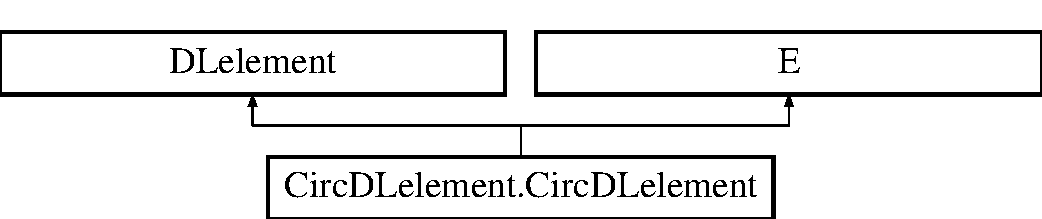
\includegraphics[height=5.000000cm]{class_circ_d_lelement_1_1_circ_d_lelement}
\end{center}
\end{figure}
\subsection*{Public Member Functions}
\begin{DoxyCompactItemize}
\item 
def \hyperlink{class_circ_d_lelement_1_1_circ_d_lelement_a9dd07008f966ac2b37cb6d678e13b27a}{\+\_\+\+\_\+init\+\_\+\+\_\+}
\begin{DoxyCompactList}\small\item\em Constructs an empty \hyperlink{class_circ_d_lelement_1_1_circ_d_lelement}{Circ\+D\+Lelement} with next and prev pointers set to itself. \end{DoxyCompactList}\item 
def \hyperlink{class_circ_d_lelement_1_1_circ_d_lelement_ab296525ea7f441251229b09645db81a4}{get\+\_\+data\+\_\+structure\+\_\+type} (self)
\begin{DoxyCompactList}\small\item\em This method gets the data structure type. \end{DoxyCompactList}\item 
def \hyperlink{class_circ_d_lelement_1_1_circ_d_lelement_ac6a27224354774b152abc3bd05bc8286}{get\+\_\+next} (self)
\begin{DoxyCompactList}\small\item\em This method returns the pointer to the next \hyperlink{namespace_d_lelement}{D\+Lelement}. \end{DoxyCompactList}\item 
def \hyperlink{class_circ_d_lelement_1_1_circ_d_lelement_afa343f86ca9a92571c2140d82b3850f0}{get\+\_\+prev} (self)
\begin{DoxyCompactList}\small\item\em This method returns the pointer to the previous \hyperlink{namespace_d_lelement}{D\+Lelement}. \end{DoxyCompactList}\end{DoxyCompactItemize}
\subsection*{Public Attributes}
\begin{DoxyCompactItemize}
\item 
\hyperlink{class_circ_d_lelement_1_1_circ_d_lelement_a58f067bcf3daa5c7a0e944bc91961af9}{next}
\item 
\hyperlink{class_circ_d_lelement_1_1_circ_d_lelement_a71d1419a7eb3687a3351e5ea0bcd55b4}{prev}
\end{DoxyCompactItemize}
\subsection*{Additional Inherited Members}


\subsection{Detailed Description}
This class can be used to instantiate Circular Doubly Linked List Elements. 

Structurally they are the same as doubly linked elements except that each node constructed with the next and the previous pointers points to itself.

User\textquotesingle{}s implementation of the circularly linked list needs to ensure that the last node\textquotesingle{}s next pointer points to the first node and the first node\textquotesingle{}s previous pointer points to the last node, as the visualization generation is dependent on this.

Elements have labels (string) that are displayed on the visualization. Elements take an generic object E as a user defined parameter, which can be any native type or object.

Elements contain a visualizer (\hyperlink{namespace_element_visualizer}{Element\+Visualizer}) object for setting visual attributes (color, shape, opacity, size), necessary for displaying them in a web browser.

Elements also have a \hyperlink{namespace_link_visualizer}{Link\+Visualizer} object that is used when they are linked to another element, appropriate for setting link attributes, between the element and its previous or next nodes.

\begin{DoxyAuthor}{Author}
Kalpathi Subramanian
\end{DoxyAuthor}
\begin{DoxyDate}{Date}
7/17/16, 1/16/17
\end{DoxyDate}

\begin{DoxyParams}{Parameters}
{\em $<$\+E$>$} & the generic parameter object that contains application specific data, defined by the user when instantiating this object.\\
\hline
\end{DoxyParams}
\begin{DoxySeeAlso}{See also}
Example Tutorial at ~\newline
 \href{http://bridgesuncc.github.io/Hello_World_Tutorials/CDLL.html}{\tt http\+://bridgesuncc.\+github.\+io/\+Hello\+\_\+\+World\+\_\+\+Tutorials/\+C\+D\+L\+L.\+html} 
\end{DoxySeeAlso}


\subsection{Constructor \& Destructor Documentation}
\hypertarget{class_circ_d_lelement_1_1_circ_d_lelement_a9dd07008f966ac2b37cb6d678e13b27a}{}\index{Circ\+D\+Lelement\+::\+Circ\+D\+Lelement@{Circ\+D\+Lelement\+::\+Circ\+D\+Lelement}!\+\_\+\+\_\+init\+\_\+\+\_\+@{\+\_\+\+\_\+init\+\_\+\+\_\+}}
\index{\+\_\+\+\_\+init\+\_\+\+\_\+@{\+\_\+\+\_\+init\+\_\+\+\_\+}!Circ\+D\+Lelement\+::\+Circ\+D\+Lelement@{Circ\+D\+Lelement\+::\+Circ\+D\+Lelement}}
\subsubsection[{\+\_\+\+\_\+init\+\_\+\+\_\+}]{\setlength{\rightskip}{0pt plus 5cm}def Circ\+D\+Lelement.\+Circ\+D\+Lelement.\+\_\+\+\_\+init\+\_\+\+\_\+ (
\begin{DoxyParamCaption}
\item[{}]{self, }
\item[{}]{e = {\ttfamily None}, }
\item[{}]{label = {\ttfamily None}, }
\item[{}]{next = {\ttfamily None}, }
\item[{}]{prev = {\ttfamily None}}
\end{DoxyParamCaption}
)}\label{class_circ_d_lelement_1_1_circ_d_lelement_a9dd07008f966ac2b37cb6d678e13b27a}


Constructs an empty \hyperlink{class_circ_d_lelement_1_1_circ_d_lelement}{Circ\+D\+Lelement} with next and prev pointers set to itself. 



\subsection{Member Function Documentation}
\hypertarget{class_circ_d_lelement_1_1_circ_d_lelement_ab296525ea7f441251229b09645db81a4}{}\index{Circ\+D\+Lelement\+::\+Circ\+D\+Lelement@{Circ\+D\+Lelement\+::\+Circ\+D\+Lelement}!get\+\_\+data\+\_\+structure\+\_\+type@{get\+\_\+data\+\_\+structure\+\_\+type}}
\index{get\+\_\+data\+\_\+structure\+\_\+type@{get\+\_\+data\+\_\+structure\+\_\+type}!Circ\+D\+Lelement\+::\+Circ\+D\+Lelement@{Circ\+D\+Lelement\+::\+Circ\+D\+Lelement}}
\subsubsection[{get\+\_\+data\+\_\+structure\+\_\+type(self)}]{\setlength{\rightskip}{0pt plus 5cm}def Circ\+D\+Lelement.\+Circ\+D\+Lelement.\+get\+\_\+data\+\_\+structure\+\_\+type (
\begin{DoxyParamCaption}
\item[{}]{self}
\end{DoxyParamCaption}
)}\label{class_circ_d_lelement_1_1_circ_d_lelement_ab296525ea7f441251229b09645db81a4}


This method gets the data structure type. 

\begin{DoxyReturn}{Returns}
The date structure type as a string 
\end{DoxyReturn}
\hypertarget{class_circ_d_lelement_1_1_circ_d_lelement_ac6a27224354774b152abc3bd05bc8286}{}\index{Circ\+D\+Lelement\+::\+Circ\+D\+Lelement@{Circ\+D\+Lelement\+::\+Circ\+D\+Lelement}!get\+\_\+next@{get\+\_\+next}}
\index{get\+\_\+next@{get\+\_\+next}!Circ\+D\+Lelement\+::\+Circ\+D\+Lelement@{Circ\+D\+Lelement\+::\+Circ\+D\+Lelement}}
\subsubsection[{get\+\_\+next(self)}]{\setlength{\rightskip}{0pt plus 5cm}def Circ\+D\+Lelement.\+Circ\+D\+Lelement.\+get\+\_\+next (
\begin{DoxyParamCaption}
\item[{}]{self}
\end{DoxyParamCaption}
)}\label{class_circ_d_lelement_1_1_circ_d_lelement_ac6a27224354774b152abc3bd05bc8286}


This method returns the pointer to the next \hyperlink{namespace_d_lelement}{D\+Lelement}. 

\begin{DoxyReturn}{Returns}
the \hyperlink{namespace_d_lelement}{D\+Lelement} assigned to the next pointer 
\end{DoxyReturn}
\hypertarget{class_circ_d_lelement_1_1_circ_d_lelement_afa343f86ca9a92571c2140d82b3850f0}{}\index{Circ\+D\+Lelement\+::\+Circ\+D\+Lelement@{Circ\+D\+Lelement\+::\+Circ\+D\+Lelement}!get\+\_\+prev@{get\+\_\+prev}}
\index{get\+\_\+prev@{get\+\_\+prev}!Circ\+D\+Lelement\+::\+Circ\+D\+Lelement@{Circ\+D\+Lelement\+::\+Circ\+D\+Lelement}}
\subsubsection[{get\+\_\+prev(self)}]{\setlength{\rightskip}{0pt plus 5cm}def Circ\+D\+Lelement.\+Circ\+D\+Lelement.\+get\+\_\+prev (
\begin{DoxyParamCaption}
\item[{}]{self}
\end{DoxyParamCaption}
)}\label{class_circ_d_lelement_1_1_circ_d_lelement_afa343f86ca9a92571c2140d82b3850f0}


This method returns the pointer to the previous \hyperlink{namespace_d_lelement}{D\+Lelement}. 

\begin{DoxyReturn}{Returns}
the \hyperlink{namespace_d_lelement}{D\+Lelement} assigned to the prev pointer 
\end{DoxyReturn}


\subsection{Member Data Documentation}
\hypertarget{class_circ_d_lelement_1_1_circ_d_lelement_a58f067bcf3daa5c7a0e944bc91961af9}{}\index{Circ\+D\+Lelement\+::\+Circ\+D\+Lelement@{Circ\+D\+Lelement\+::\+Circ\+D\+Lelement}!next@{next}}
\index{next@{next}!Circ\+D\+Lelement\+::\+Circ\+D\+Lelement@{Circ\+D\+Lelement\+::\+Circ\+D\+Lelement}}
\subsubsection[{next}]{\setlength{\rightskip}{0pt plus 5cm}Circ\+D\+Lelement.\+Circ\+D\+Lelement.\+next}\label{class_circ_d_lelement_1_1_circ_d_lelement_a58f067bcf3daa5c7a0e944bc91961af9}
\hypertarget{class_circ_d_lelement_1_1_circ_d_lelement_a71d1419a7eb3687a3351e5ea0bcd55b4}{}\index{Circ\+D\+Lelement\+::\+Circ\+D\+Lelement@{Circ\+D\+Lelement\+::\+Circ\+D\+Lelement}!prev@{prev}}
\index{prev@{prev}!Circ\+D\+Lelement\+::\+Circ\+D\+Lelement@{Circ\+D\+Lelement\+::\+Circ\+D\+Lelement}}
\subsubsection[{prev}]{\setlength{\rightskip}{0pt plus 5cm}Circ\+D\+Lelement.\+Circ\+D\+Lelement.\+prev}\label{class_circ_d_lelement_1_1_circ_d_lelement_a71d1419a7eb3687a3351e5ea0bcd55b4}


The documentation for this class was generated from the following file\+:\begin{DoxyCompactItemize}
\item 
/\+Users/krs/gr/bridges/bridges17/python/src/\hyperlink{_circ_d_lelement_8py}{Circ\+D\+Lelement.\+py}\end{DoxyCompactItemize}

\hypertarget{class_circ_s_lelement_1_1_circ_s_lelement}{}\section{Circ\+S\+Lelement.\+Circ\+S\+Lelement Class Reference}
\label{class_circ_s_lelement_1_1_circ_s_lelement}\index{Circ\+S\+Lelement.\+Circ\+S\+Lelement@{Circ\+S\+Lelement.\+Circ\+S\+Lelement}}


This class can be used to instantiate Singly Linked Circular List Elements.  


Inheritance diagram for Circ\+S\+Lelement.\+Circ\+S\+Lelement\+:\begin{figure}[H]
\begin{center}
\leavevmode
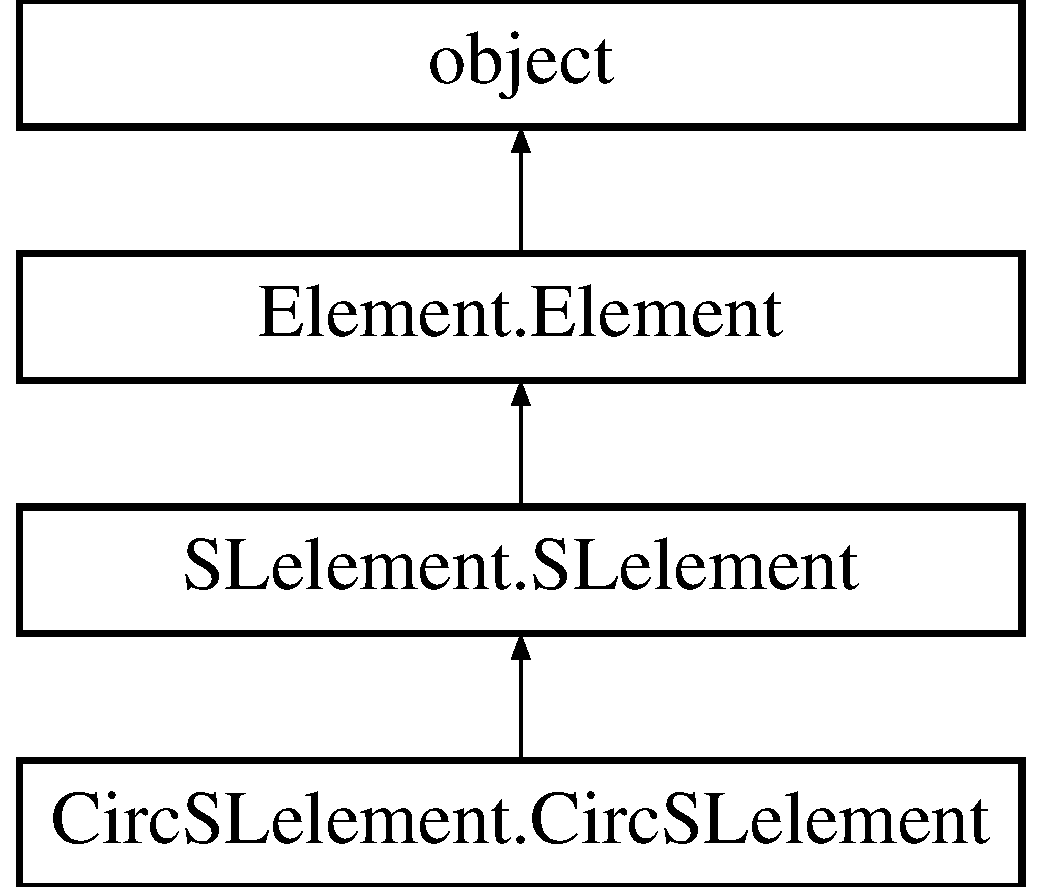
\includegraphics[height=4.000000cm]{class_circ_s_lelement_1_1_circ_s_lelement}
\end{center}
\end{figure}
\subsection*{Public Member Functions}
\begin{DoxyCompactItemize}
\item 
def \hyperlink{class_circ_s_lelement_1_1_circ_s_lelement_a4e75a1838fda7127fa5b1ae37b7c3a97}{\+\_\+\+\_\+init\+\_\+\+\_\+}
\begin{DoxyCompactList}\small\item\em This constructor creates an \hyperlink{class_circ_s_lelement_1_1_circ_s_lelement}{Circ\+S\+Lelement} object and sets its next pointer to itself. \end{DoxyCompactList}\item 
def \hyperlink{class_circ_s_lelement_1_1_circ_s_lelement_affcfd41e826ec28da6d3f3b89463457a}{get\+\_\+data\+\_\+structure\+\_\+type} (self)
\begin{DoxyCompactList}\small\item\em This method gets the data structure type. \end{DoxyCompactList}\item 
def \hyperlink{class_circ_s_lelement_1_1_circ_s_lelement_ae4b14fdaf7123cde09b78f8b65101c7c}{get\+\_\+next} (self)
\begin{DoxyCompactList}\small\item\em Retrieves the next \hyperlink{class_circ_s_lelement_1_1_circ_s_lelement}{Circ\+S\+Lelement}. \end{DoxyCompactList}\item 
def \hyperlink{class_circ_s_lelement_1_1_circ_s_lelement_ae75eb1b91bebd77b39fdb2c3345ded4b}{\+\_\+\+\_\+str\+\_\+\+\_\+} (self)
\end{DoxyCompactItemize}
\subsection*{Additional Inherited Members}


\subsection{Detailed Description}
This class can be used to instantiate Singly Linked Circular List Elements. 

Structurally they are the same as singly linked elements except that each node constructed with the next point pointing to itself; User\textquotesingle{}s implementation of the circularly linked list needs to ensure that the last node points to first node of the list, as the visualization generation is dependent on this.

Elements have labels (string) that are displayed on the visualization. Elements take an generic object as a user defined parameter, E, which can be any native type or object.

Elements contains a visualizer (\hyperlink{namespace_element_visualizer}{Element\+Visualizer}) object for setting visual attributes (color, shape, opacity, size), necessary for displaying them in a web browser.

Elements also have a \hyperlink{namespace_link_visualizer}{Link\+Visualizer} object that is used when they are linked to another element, appropriate for setting link attributes, between an element and its next element.

\begin{DoxyAuthor}{Author}
Kalpathi Subramanian
\end{DoxyAuthor}
\begin{DoxyDate}{Date}
6/22/16, 1/7/17, 5/17/17
\end{DoxyDate}

\begin{DoxyParams}{Parameters}
{\em $<$\+E$>$} & the generic parameter that is defined by the application\\
\hline
\end{DoxyParams}
\begin{DoxySeeAlso}{See also}
Example Tutorial at ~\newline
 \href{http://bridgesuncc.github.io/Hello_World_Tutorials/CSLL.html}{\tt http\+://bridgesuncc.\+github.\+io/\+Hello\+\_\+\+World\+\_\+\+Tutorials/\+C\+S\+L\+L.\+html} 
\end{DoxySeeAlso}


\subsection{Constructor \& Destructor Documentation}
\hypertarget{class_circ_s_lelement_1_1_circ_s_lelement_a4e75a1838fda7127fa5b1ae37b7c3a97}{}\index{Circ\+S\+Lelement\+::\+Circ\+S\+Lelement@{Circ\+S\+Lelement\+::\+Circ\+S\+Lelement}!\+\_\+\+\_\+init\+\_\+\+\_\+@{\+\_\+\+\_\+init\+\_\+\+\_\+}}
\index{\+\_\+\+\_\+init\+\_\+\+\_\+@{\+\_\+\+\_\+init\+\_\+\+\_\+}!Circ\+S\+Lelement\+::\+Circ\+S\+Lelement@{Circ\+S\+Lelement\+::\+Circ\+S\+Lelement}}
\subsubsection[{\+\_\+\+\_\+init\+\_\+\+\_\+}]{\setlength{\rightskip}{0pt plus 5cm}def Circ\+S\+Lelement.\+Circ\+S\+Lelement.\+\_\+\+\_\+init\+\_\+\+\_\+ (
\begin{DoxyParamCaption}
\item[{}]{self, }
\item[{}]{e = {\ttfamily None}, }
\item[{}]{label = {\ttfamily None}, }
\item[{}]{next = {\ttfamily None}}
\end{DoxyParamCaption}
)}\label{class_circ_s_lelement_1_1_circ_s_lelement_a4e75a1838fda7127fa5b1ae37b7c3a97}


This constructor creates an \hyperlink{class_circ_s_lelement_1_1_circ_s_lelement}{Circ\+S\+Lelement} object and sets its next pointer to itself. 



\subsection{Member Function Documentation}
\hypertarget{class_circ_s_lelement_1_1_circ_s_lelement_ae75eb1b91bebd77b39fdb2c3345ded4b}{}\index{Circ\+S\+Lelement\+::\+Circ\+S\+Lelement@{Circ\+S\+Lelement\+::\+Circ\+S\+Lelement}!\+\_\+\+\_\+str\+\_\+\+\_\+@{\+\_\+\+\_\+str\+\_\+\+\_\+}}
\index{\+\_\+\+\_\+str\+\_\+\+\_\+@{\+\_\+\+\_\+str\+\_\+\+\_\+}!Circ\+S\+Lelement\+::\+Circ\+S\+Lelement@{Circ\+S\+Lelement\+::\+Circ\+S\+Lelement}}
\subsubsection[{\+\_\+\+\_\+str\+\_\+\+\_\+(self)}]{\setlength{\rightskip}{0pt plus 5cm}def Circ\+S\+Lelement.\+Circ\+S\+Lelement.\+\_\+\+\_\+str\+\_\+\+\_\+ (
\begin{DoxyParamCaption}
\item[{}]{self}
\end{DoxyParamCaption}
)}\label{class_circ_s_lelement_1_1_circ_s_lelement_ae75eb1b91bebd77b39fdb2c3345ded4b}
\hypertarget{class_circ_s_lelement_1_1_circ_s_lelement_affcfd41e826ec28da6d3f3b89463457a}{}\index{Circ\+S\+Lelement\+::\+Circ\+S\+Lelement@{Circ\+S\+Lelement\+::\+Circ\+S\+Lelement}!get\+\_\+data\+\_\+structure\+\_\+type@{get\+\_\+data\+\_\+structure\+\_\+type}}
\index{get\+\_\+data\+\_\+structure\+\_\+type@{get\+\_\+data\+\_\+structure\+\_\+type}!Circ\+S\+Lelement\+::\+Circ\+S\+Lelement@{Circ\+S\+Lelement\+::\+Circ\+S\+Lelement}}
\subsubsection[{get\+\_\+data\+\_\+structure\+\_\+type(self)}]{\setlength{\rightskip}{0pt plus 5cm}def Circ\+S\+Lelement.\+Circ\+S\+Lelement.\+get\+\_\+data\+\_\+structure\+\_\+type (
\begin{DoxyParamCaption}
\item[{}]{self}
\end{DoxyParamCaption}
)}\label{class_circ_s_lelement_1_1_circ_s_lelement_affcfd41e826ec28da6d3f3b89463457a}


This method gets the data structure type. 

\begin{DoxyReturn}{Returns}
The date structure type as a string 
\end{DoxyReturn}
\hypertarget{class_circ_s_lelement_1_1_circ_s_lelement_ae4b14fdaf7123cde09b78f8b65101c7c}{}\index{Circ\+S\+Lelement\+::\+Circ\+S\+Lelement@{Circ\+S\+Lelement\+::\+Circ\+S\+Lelement}!get\+\_\+next@{get\+\_\+next}}
\index{get\+\_\+next@{get\+\_\+next}!Circ\+S\+Lelement\+::\+Circ\+S\+Lelement@{Circ\+S\+Lelement\+::\+Circ\+S\+Lelement}}
\subsubsection[{get\+\_\+next(self)}]{\setlength{\rightskip}{0pt plus 5cm}def Circ\+S\+Lelement.\+Circ\+S\+Lelement.\+get\+\_\+next (
\begin{DoxyParamCaption}
\item[{}]{self}
\end{DoxyParamCaption}
)}\label{class_circ_s_lelement_1_1_circ_s_lelement_ae4b14fdaf7123cde09b78f8b65101c7c}


Retrieves the next \hyperlink{class_circ_s_lelement_1_1_circ_s_lelement}{Circ\+S\+Lelement}. 

\begin{DoxyReturn}{Returns}
Circ\+S\+Lelement$<$\+E$>$ assigned to next 
\end{DoxyReturn}


The documentation for this class was generated from the following file\+:\begin{DoxyCompactItemize}
\item 
/\+Users/krs/gr/bridges/bridges17/python/src/\hyperlink{_circ_s_lelement_8py}{Circ\+S\+Lelement.\+py}\end{DoxyCompactItemize}

\hypertarget{class_color_1_1_color}{}\section{Color.\+Color Class Reference}
\label{class_color_1_1_color}\index{Color.\+Color@{Color.\+Color}}


This class is used to represent colors in B\+R\+I\+D\+G\+ES.  


Inheritance diagram for Color.\+Color\+:\begin{figure}[H]
\begin{center}
\leavevmode
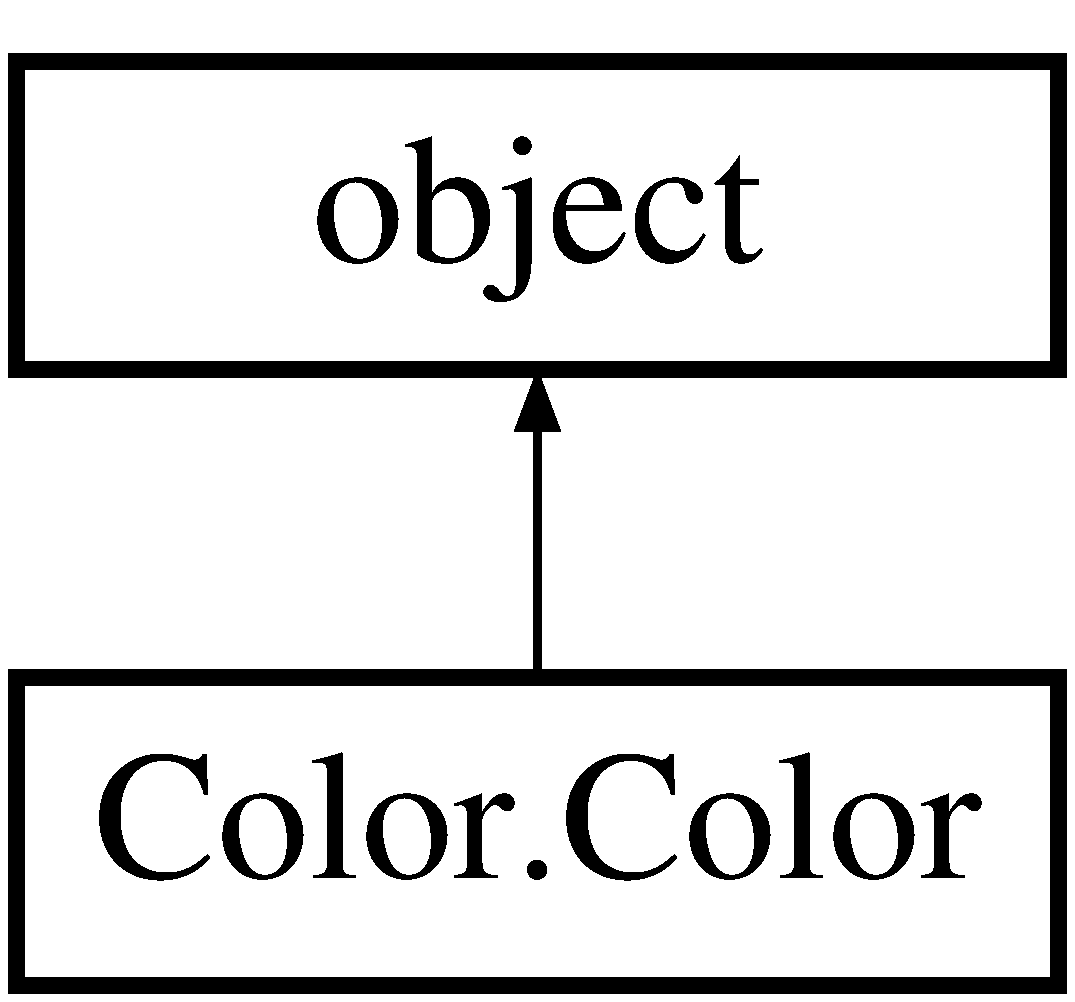
\includegraphics[height=2.000000cm]{class_color_1_1_color}
\end{center}
\end{figure}
\subsection*{Public Member Functions}
\begin{DoxyCompactItemize}
\item 
def \hyperlink{class_color_1_1_color_a54e49ab0562f1754ee309481f889734b}{\+\_\+\+\_\+init\+\_\+\+\_\+} (self)
\begin{DoxyCompactList}\small\item\em Constructors. \end{DoxyCompactList}\item 
def \hyperlink{class_color_1_1_color_afa03ead21a88146b5ddbc89a53ffcda8}{set\+Color} (self, r, g, b, a)
\begin{DoxyCompactList}\small\item\em sets color to the given r, g, b, a components \end{DoxyCompactList}\item 
def \hyperlink{class_color_1_1_color_ac9000b54846a4d69171dd81172e53f96}{set\+Red} (self, r)
\begin{DoxyCompactList}\small\item\em sets the red component \end{DoxyCompactList}\item 
def \hyperlink{class_color_1_1_color_af714dcb6373051df8548d41ea4160896}{get\+Red} (self)
\begin{DoxyCompactList}\small\item\em gets the red component \end{DoxyCompactList}\item 
def \hyperlink{class_color_1_1_color_a3ea676f0ace46e02292527acc7915d0b}{set\+Green} (self, g)
\begin{DoxyCompactList}\small\item\em sets the green component \end{DoxyCompactList}\item 
def \hyperlink{class_color_1_1_color_acf5013ef6e09f0d3a86b6f4044e60abb}{get\+Green} (self)
\begin{DoxyCompactList}\small\item\em gets the green component \end{DoxyCompactList}\item 
def \hyperlink{class_color_1_1_color_a2fad4bb66a79ba2b51acfa875f376c3b}{set\+Blue} (self, b)
\begin{DoxyCompactList}\small\item\em sets the blue component \end{DoxyCompactList}\item 
def \hyperlink{class_color_1_1_color_a00ee33a98b9243f68dd02d4882698ff6}{get\+Blue} (self)
\begin{DoxyCompactList}\small\item\em gets the blue component \end{DoxyCompactList}\item 
def \hyperlink{class_color_1_1_color_a794d9889de916d2d45f29437547feddd}{set\+Alpha} (self, a)
\begin{DoxyCompactList}\small\item\em sets the alpha(opacity) component \end{DoxyCompactList}\item 
def \hyperlink{class_color_1_1_color_a2d8eedef0a8731d96e2a1f802d04b42e}{get\+Alpha} (self)
\begin{DoxyCompactList}\small\item\em gets the alpha component \end{DoxyCompactList}\item 
def \hyperlink{class_color_1_1_color_ab17d74d2318751b06e1fc9688f7ee273}{set\+Color\+\_\+0} (self, col\+\_\+name)
\begin{DoxyCompactList}\small\item\em sets the color to the R\+G\+BA components given the color name \end{DoxyCompactList}\end{DoxyCompactItemize}
\subsection*{Static Public Attributes}
\begin{DoxyCompactItemize}
\item 
\hyperlink{class_color_1_1_color_ad6b9578f975c4f066a1e34dff6ac557a}{red} = int()
\item 
\hyperlink{class_color_1_1_color_a608f39a75b991c1ffda8bd91d9744d2b}{green} = int()
\item 
\hyperlink{class_color_1_1_color_aae0c5d7ff0540d207fac048534b7e8bf}{blue} = int()
\item 
\hyperlink{class_color_1_1_color_a27e8f74882075cc184a9bbc2da65f8a3}{alpha} = float()
\item 
\hyperlink{class_color_1_1_color_ade3e7466d27087359ca123a8406c6f3f}{Color\+Names} = Hash\+Map()
\end{DoxyCompactItemize}


\subsection{Detailed Description}
This class is used to represent colors in B\+R\+I\+D\+G\+ES. 

We use an R\+G\+BA model to represent colors, with each component in the range 0-\/255. B\+R\+I\+D\+G\+ES also supports named colors for user convenience, but these are converted into \mbox{[}R\+G\+BA\mbox{]} prior to transmission to the server for visualization.

\begin{DoxyAuthor}{Author}
K.\+R. Subramanian, 
\end{DoxyAuthor}
\begin{DoxyDate}{Date}
7/14/16\begin{DoxyVerb}generated source for class Color \end{DoxyVerb}
 
\end{DoxyDate}


\subsection{Constructor \& Destructor Documentation}
\hypertarget{class_color_1_1_color_a54e49ab0562f1754ee309481f889734b}{}\label{class_color_1_1_color_a54e49ab0562f1754ee309481f889734b} 
\index{Color\+::\+Color@{Color\+::\+Color}!\+\_\+\+\_\+init\+\_\+\+\_\+@{\+\_\+\+\_\+init\+\_\+\+\_\+}}
\index{\+\_\+\+\_\+init\+\_\+\+\_\+@{\+\_\+\+\_\+init\+\_\+\+\_\+}!Color\+::\+Color@{Color\+::\+Color}}
\subsubsection{\texorpdfstring{\+\_\+\+\_\+init\+\_\+\+\_\+()}{\_\_init\_\_()}}
{\footnotesize\ttfamily def Color.\+Color.\+\_\+\+\_\+init\+\_\+\+\_\+ (\begin{DoxyParamCaption}\item[{}]{self }\end{DoxyParamCaption})}



Constructors. 

\begin{DoxyVerb}generated source for method __init__ \end{DoxyVerb}
 

\subsection{Member Function Documentation}
\hypertarget{class_color_1_1_color_a2d8eedef0a8731d96e2a1f802d04b42e}{}\label{class_color_1_1_color_a2d8eedef0a8731d96e2a1f802d04b42e} 
\index{Color\+::\+Color@{Color\+::\+Color}!get\+Alpha@{get\+Alpha}}
\index{get\+Alpha@{get\+Alpha}!Color\+::\+Color@{Color\+::\+Color}}
\subsubsection{\texorpdfstring{get\+Alpha()}{getAlpha()}}
{\footnotesize\ttfamily def Color.\+Color.\+get\+Alpha (\begin{DoxyParamCaption}\item[{}]{self }\end{DoxyParamCaption})}



gets the alpha component 

\begin{DoxyReturn}{Returns}
alpha -\/ returns the alpha(opacity) component of the color\begin{DoxyVerb}generated source for method getAlpha \end{DoxyVerb}
 
\end{DoxyReturn}
\hypertarget{class_color_1_1_color_a00ee33a98b9243f68dd02d4882698ff6}{}\label{class_color_1_1_color_a00ee33a98b9243f68dd02d4882698ff6} 
\index{Color\+::\+Color@{Color\+::\+Color}!get\+Blue@{get\+Blue}}
\index{get\+Blue@{get\+Blue}!Color\+::\+Color@{Color\+::\+Color}}
\subsubsection{\texorpdfstring{get\+Blue()}{getBlue()}}
{\footnotesize\ttfamily def Color.\+Color.\+get\+Blue (\begin{DoxyParamCaption}\item[{}]{self }\end{DoxyParamCaption})}



gets the blue component 

\begin{DoxyReturn}{Returns}
blue -\/ returns the blue component of the color\begin{DoxyVerb}generated source for method getBlue \end{DoxyVerb}
 
\end{DoxyReturn}
\hypertarget{class_color_1_1_color_acf5013ef6e09f0d3a86b6f4044e60abb}{}\label{class_color_1_1_color_acf5013ef6e09f0d3a86b6f4044e60abb} 
\index{Color\+::\+Color@{Color\+::\+Color}!get\+Green@{get\+Green}}
\index{get\+Green@{get\+Green}!Color\+::\+Color@{Color\+::\+Color}}
\subsubsection{\texorpdfstring{get\+Green()}{getGreen()}}
{\footnotesize\ttfamily def Color.\+Color.\+get\+Green (\begin{DoxyParamCaption}\item[{}]{self }\end{DoxyParamCaption})}



gets the green component 

\begin{DoxyReturn}{Returns}
green -\/ returns the green component of the color\begin{DoxyVerb}generated source for method getGreen \end{DoxyVerb}
 
\end{DoxyReturn}
\hypertarget{class_color_1_1_color_af714dcb6373051df8548d41ea4160896}{}\label{class_color_1_1_color_af714dcb6373051df8548d41ea4160896} 
\index{Color\+::\+Color@{Color\+::\+Color}!get\+Red@{get\+Red}}
\index{get\+Red@{get\+Red}!Color\+::\+Color@{Color\+::\+Color}}
\subsubsection{\texorpdfstring{get\+Red()}{getRed()}}
{\footnotesize\ttfamily def Color.\+Color.\+get\+Red (\begin{DoxyParamCaption}\item[{}]{self }\end{DoxyParamCaption})}



gets the red component 

\begin{DoxyReturn}{Returns}
red -\/ returns the red component of the color\begin{DoxyVerb}generated source for method getRed \end{DoxyVerb}
 
\end{DoxyReturn}
\hypertarget{class_color_1_1_color_a794d9889de916d2d45f29437547feddd}{}\label{class_color_1_1_color_a794d9889de916d2d45f29437547feddd} 
\index{Color\+::\+Color@{Color\+::\+Color}!set\+Alpha@{set\+Alpha}}
\index{set\+Alpha@{set\+Alpha}!Color\+::\+Color@{Color\+::\+Color}}
\subsubsection{\texorpdfstring{set\+Alpha()}{setAlpha()}}
{\footnotesize\ttfamily def Color.\+Color.\+set\+Alpha (\begin{DoxyParamCaption}\item[{}]{self,  }\item[{}]{a }\end{DoxyParamCaption})}



sets the alpha(opacity) component 


\begin{DoxyParams}{Parameters}
{\em a} & -\/ checked to be in the range 0-\/255\begin{DoxyVerb}generated source for method setAlpha \end{DoxyVerb}
 \\
\hline
\end{DoxyParams}
\hypertarget{class_color_1_1_color_a2fad4bb66a79ba2b51acfa875f376c3b}{}\label{class_color_1_1_color_a2fad4bb66a79ba2b51acfa875f376c3b} 
\index{Color\+::\+Color@{Color\+::\+Color}!set\+Blue@{set\+Blue}}
\index{set\+Blue@{set\+Blue}!Color\+::\+Color@{Color\+::\+Color}}
\subsubsection{\texorpdfstring{set\+Blue()}{setBlue()}}
{\footnotesize\ttfamily def Color.\+Color.\+set\+Blue (\begin{DoxyParamCaption}\item[{}]{self,  }\item[{}]{b }\end{DoxyParamCaption})}



sets the blue component 


\begin{DoxyParams}{Parameters}
{\em b} & -\/ checked to be in the range 0-\/255\begin{DoxyVerb}generated source for method setBlue \end{DoxyVerb}
 \\
\hline
\end{DoxyParams}
\hypertarget{class_color_1_1_color_afa03ead21a88146b5ddbc89a53ffcda8}{}\label{class_color_1_1_color_afa03ead21a88146b5ddbc89a53ffcda8} 
\index{Color\+::\+Color@{Color\+::\+Color}!set\+Color@{set\+Color}}
\index{set\+Color@{set\+Color}!Color\+::\+Color@{Color\+::\+Color}}
\subsubsection{\texorpdfstring{set\+Color()}{setColor()}}
{\footnotesize\ttfamily def Color.\+Color.\+set\+Color (\begin{DoxyParamCaption}\item[{}]{self,  }\item[{}]{r,  }\item[{}]{g,  }\item[{}]{b,  }\item[{}]{a }\end{DoxyParamCaption})}



sets color to the given r, g, b, a components 


\begin{DoxyParams}{Parameters}
{\em r,g,b,a} & -\/ checked to be in the range 0-\/255\begin{DoxyVerb}generated source for method setColor \end{DoxyVerb}
 \\
\hline
\end{DoxyParams}
\hypertarget{class_color_1_1_color_ab17d74d2318751b06e1fc9688f7ee273}{}\label{class_color_1_1_color_ab17d74d2318751b06e1fc9688f7ee273} 
\index{Color\+::\+Color@{Color\+::\+Color}!set\+Color\+\_\+0@{set\+Color\+\_\+0}}
\index{set\+Color\+\_\+0@{set\+Color\+\_\+0}!Color\+::\+Color@{Color\+::\+Color}}
\subsubsection{\texorpdfstring{set\+Color\+\_\+0()}{setColor\_0()}}
{\footnotesize\ttfamily def Color.\+Color.\+set\+Color\+\_\+0 (\begin{DoxyParamCaption}\item[{}]{self,  }\item[{}]{col\+\_\+name }\end{DoxyParamCaption})}



sets the color to the R\+G\+BA components given the color name 


\begin{DoxyParams}{Parameters}
{\em col\+\_\+name} & color name\begin{DoxyVerb}generated source for method setColor_0 \end{DoxyVerb}
 \\
\hline
\end{DoxyParams}
\hypertarget{class_color_1_1_color_a3ea676f0ace46e02292527acc7915d0b}{}\label{class_color_1_1_color_a3ea676f0ace46e02292527acc7915d0b} 
\index{Color\+::\+Color@{Color\+::\+Color}!set\+Green@{set\+Green}}
\index{set\+Green@{set\+Green}!Color\+::\+Color@{Color\+::\+Color}}
\subsubsection{\texorpdfstring{set\+Green()}{setGreen()}}
{\footnotesize\ttfamily def Color.\+Color.\+set\+Green (\begin{DoxyParamCaption}\item[{}]{self,  }\item[{}]{g }\end{DoxyParamCaption})}



sets the green component 


\begin{DoxyParams}{Parameters}
{\em g} & -\/ checked to be in the range 0-\/255\begin{DoxyVerb}generated source for method setGreen \end{DoxyVerb}
 \\
\hline
\end{DoxyParams}
\hypertarget{class_color_1_1_color_ac9000b54846a4d69171dd81172e53f96}{}\label{class_color_1_1_color_ac9000b54846a4d69171dd81172e53f96} 
\index{Color\+::\+Color@{Color\+::\+Color}!set\+Red@{set\+Red}}
\index{set\+Red@{set\+Red}!Color\+::\+Color@{Color\+::\+Color}}
\subsubsection{\texorpdfstring{set\+Red()}{setRed()}}
{\footnotesize\ttfamily def Color.\+Color.\+set\+Red (\begin{DoxyParamCaption}\item[{}]{self,  }\item[{}]{r }\end{DoxyParamCaption})}



sets the red component 


\begin{DoxyParams}{Parameters}
{\em r} & -\/ checked to be in the range 0-\/255\begin{DoxyVerb}generated source for method setRed \end{DoxyVerb}
 \\
\hline
\end{DoxyParams}


\subsection{Member Data Documentation}
\hypertarget{class_color_1_1_color_a27e8f74882075cc184a9bbc2da65f8a3}{}\label{class_color_1_1_color_a27e8f74882075cc184a9bbc2da65f8a3} 
\index{Color\+::\+Color@{Color\+::\+Color}!alpha@{alpha}}
\index{alpha@{alpha}!Color\+::\+Color@{Color\+::\+Color}}
\subsubsection{\texorpdfstring{alpha}{alpha}}
{\footnotesize\ttfamily Color.\+Color.\+alpha = float()\hspace{0.3cm}{\ttfamily [static]}}

\hypertarget{class_color_1_1_color_aae0c5d7ff0540d207fac048534b7e8bf}{}\label{class_color_1_1_color_aae0c5d7ff0540d207fac048534b7e8bf} 
\index{Color\+::\+Color@{Color\+::\+Color}!blue@{blue}}
\index{blue@{blue}!Color\+::\+Color@{Color\+::\+Color}}
\subsubsection{\texorpdfstring{blue}{blue}}
{\footnotesize\ttfamily Color.\+Color.\+blue = int()\hspace{0.3cm}{\ttfamily [static]}}

\hypertarget{class_color_1_1_color_ade3e7466d27087359ca123a8406c6f3f}{}\label{class_color_1_1_color_ade3e7466d27087359ca123a8406c6f3f} 
\index{Color\+::\+Color@{Color\+::\+Color}!Color\+Names@{Color\+Names}}
\index{Color\+Names@{Color\+Names}!Color\+::\+Color@{Color\+::\+Color}}
\subsubsection{\texorpdfstring{Color\+Names}{ColorNames}}
{\footnotesize\ttfamily Color.\+Color.\+Color\+Names = Hash\+Map()\hspace{0.3cm}{\ttfamily [static]}}

\hypertarget{class_color_1_1_color_a608f39a75b991c1ffda8bd91d9744d2b}{}\label{class_color_1_1_color_a608f39a75b991c1ffda8bd91d9744d2b} 
\index{Color\+::\+Color@{Color\+::\+Color}!green@{green}}
\index{green@{green}!Color\+::\+Color@{Color\+::\+Color}}
\subsubsection{\texorpdfstring{green}{green}}
{\footnotesize\ttfamily Color.\+Color.\+green = int()\hspace{0.3cm}{\ttfamily [static]}}

\hypertarget{class_color_1_1_color_ad6b9578f975c4f066a1e34dff6ac557a}{}\label{class_color_1_1_color_ad6b9578f975c4f066a1e34dff6ac557a} 
\index{Color\+::\+Color@{Color\+::\+Color}!red@{red}}
\index{red@{red}!Color\+::\+Color@{Color\+::\+Color}}
\subsubsection{\texorpdfstring{red}{red}}
{\footnotesize\ttfamily Color.\+Color.\+red = int()\hspace{0.3cm}{\ttfamily [static]}}



The documentation for this class was generated from the following file\+:\begin{DoxyCompactItemize}
\item 
/\+Users/kalpathi/gr/bridges/client/python/src/\hyperlink{_color_8py}{Color.\+py}\end{DoxyCompactItemize}

\hypertarget{class_connector_1_1_connector}{}\section{Connector.\+Connector Class Reference}
\label{class_connector_1_1_connector}\index{Connector.\+Connector@{Connector.\+Connector}}
\subsection*{Public Member Functions}
\begin{DoxyCompactItemize}
\item 
def \hyperlink{class_connector_1_1_connector_a32f8a0c9743ebf1c7dc1e6456d98118b}{\+\_\+\+\_\+init\+\_\+\+\_\+} (self, \hyperlink{class_connector_1_1_connector_a68fc67f443c908108b479c2e0827c321}{key}, \hyperlink{class_connector_1_1_connector_a9c6f760e8cf57a5392c54783046f156f}{username})
\item 
def \hyperlink{class_connector_1_1_connector_ac0d10fd60e38dd5eb3758575118c6680}{set\+\_\+server} (self, server)
\item 
def \hyperlink{class_connector_1_1_connector_a4bd973d97cc89b0ebed4b72e1e996b18}{set\+\_\+server\+\_\+url} (self, \hyperlink{class_connector_1_1_connector_aee36fe395f89b6b4712cfc99f273bfa1}{server\+\_\+url})
\item 
def \hyperlink{class_connector_1_1_connector_a2216cb3f761ca30ffee9c1cc9583e7b3}{get\+\_\+server\+\_\+url} (self)
\item 
def \hyperlink{class_connector_1_1_connector_af97a62f3ee2ac6f649251e2bbc14c32d}{post} (self, url, data)
\item 
def \hyperlink{class_connector_1_1_connector_a8dcd72145102381f203c0c2f8ea457d6}{prepare} (self, url)
\end{DoxyCompactItemize}
\subsection*{Public Attributes}
\begin{DoxyCompactItemize}
\item 
\hyperlink{class_connector_1_1_connector_a0130afa02e9d0d734fe31122d4f33f9d}{key}
\item 
\hyperlink{class_connector_1_1_connector_ace64a2a0c54ce06f70ee2b444d2e6f9d}{username}
\item 
\hyperlink{class_connector_1_1_connector_a0d600c0a34c2393eb6c5cbf80c5110d6}{server\+\_\+url}
\end{DoxyCompactItemize}
\subsection*{Static Public Attributes}
\begin{DoxyCompactItemize}
\item 
string \hyperlink{class_connector_1_1_connector_aee36fe395f89b6b4712cfc99f273bfa1}{server\+\_\+url} = \char`\"{}http\+://bridges-\/cs.\+herokuapp.\+com\char`\"{}
\item 
string \hyperlink{class_connector_1_1_connector_a4ab32a04d6571d5e43c7b3f4f4c5f974}{server\+\_\+type} = \char`\"{}application\char`\"{}
\item 
string \hyperlink{class_connector_1_1_connector_a68fc67f443c908108b479c2e0827c321}{key} = \char`\"{}\char`\"{}
\item 
string \hyperlink{class_connector_1_1_connector_a9c6f760e8cf57a5392c54783046f156f}{username} = \char`\"{}\char`\"{}
\item 
int \hyperlink{class_connector_1_1_connector_a6b8474acba627274c827ec8926c643cc}{pattern\+\_\+found} = 0
\item 
\hyperlink{class_connector_1_1_connector_a0b468d0c0dcb5eef9ff8dc77941abc3e}{debug} = False
\end{DoxyCompactItemize}


\subsection{Constructor \& Destructor Documentation}
\hypertarget{class_connector_1_1_connector_a32f8a0c9743ebf1c7dc1e6456d98118b}{}\index{Connector\+::\+Connector@{Connector\+::\+Connector}!\+\_\+\+\_\+init\+\_\+\+\_\+@{\+\_\+\+\_\+init\+\_\+\+\_\+}}
\index{\+\_\+\+\_\+init\+\_\+\+\_\+@{\+\_\+\+\_\+init\+\_\+\+\_\+}!Connector\+::\+Connector@{Connector\+::\+Connector}}
\subsubsection[{\+\_\+\+\_\+init\+\_\+\+\_\+(self, key, username)}]{\setlength{\rightskip}{0pt plus 5cm}def Connector.\+Connector.\+\_\+\+\_\+init\+\_\+\+\_\+ (
\begin{DoxyParamCaption}
\item[{}]{self, }
\item[{}]{key, }
\item[{}]{username}
\end{DoxyParamCaption}
)}\label{class_connector_1_1_connector_a32f8a0c9743ebf1c7dc1e6456d98118b}


\subsection{Member Function Documentation}
\hypertarget{class_connector_1_1_connector_a2216cb3f761ca30ffee9c1cc9583e7b3}{}\index{Connector\+::\+Connector@{Connector\+::\+Connector}!get\+\_\+server\+\_\+url@{get\+\_\+server\+\_\+url}}
\index{get\+\_\+server\+\_\+url@{get\+\_\+server\+\_\+url}!Connector\+::\+Connector@{Connector\+::\+Connector}}
\subsubsection[{get\+\_\+server\+\_\+url(self)}]{\setlength{\rightskip}{0pt plus 5cm}def Connector.\+Connector.\+get\+\_\+server\+\_\+url (
\begin{DoxyParamCaption}
\item[{}]{self}
\end{DoxyParamCaption}
)}\label{class_connector_1_1_connector_a2216cb3f761ca30ffee9c1cc9583e7b3}
\hypertarget{class_connector_1_1_connector_af97a62f3ee2ac6f649251e2bbc14c32d}{}\index{Connector\+::\+Connector@{Connector\+::\+Connector}!post@{post}}
\index{post@{post}!Connector\+::\+Connector@{Connector\+::\+Connector}}
\subsubsection[{post(self, url, data)}]{\setlength{\rightskip}{0pt plus 5cm}def Connector.\+Connector.\+post (
\begin{DoxyParamCaption}
\item[{}]{self, }
\item[{}]{url, }
\item[{}]{data}
\end{DoxyParamCaption}
)}\label{class_connector_1_1_connector_af97a62f3ee2ac6f649251e2bbc14c32d}
\hypertarget{class_connector_1_1_connector_a8dcd72145102381f203c0c2f8ea457d6}{}\index{Connector\+::\+Connector@{Connector\+::\+Connector}!prepare@{prepare}}
\index{prepare@{prepare}!Connector\+::\+Connector@{Connector\+::\+Connector}}
\subsubsection[{prepare(self, url)}]{\setlength{\rightskip}{0pt plus 5cm}def Connector.\+Connector.\+prepare (
\begin{DoxyParamCaption}
\item[{}]{self, }
\item[{}]{url}
\end{DoxyParamCaption}
)}\label{class_connector_1_1_connector_a8dcd72145102381f203c0c2f8ea457d6}
\hypertarget{class_connector_1_1_connector_ac0d10fd60e38dd5eb3758575118c6680}{}\index{Connector\+::\+Connector@{Connector\+::\+Connector}!set\+\_\+server@{set\+\_\+server}}
\index{set\+\_\+server@{set\+\_\+server}!Connector\+::\+Connector@{Connector\+::\+Connector}}
\subsubsection[{set\+\_\+server(self, server)}]{\setlength{\rightskip}{0pt plus 5cm}def Connector.\+Connector.\+set\+\_\+server (
\begin{DoxyParamCaption}
\item[{}]{self, }
\item[{}]{server}
\end{DoxyParamCaption}
)}\label{class_connector_1_1_connector_ac0d10fd60e38dd5eb3758575118c6680}
\hypertarget{class_connector_1_1_connector_a4bd973d97cc89b0ebed4b72e1e996b18}{}\index{Connector\+::\+Connector@{Connector\+::\+Connector}!set\+\_\+server\+\_\+url@{set\+\_\+server\+\_\+url}}
\index{set\+\_\+server\+\_\+url@{set\+\_\+server\+\_\+url}!Connector\+::\+Connector@{Connector\+::\+Connector}}
\subsubsection[{set\+\_\+server\+\_\+url(self, server\+\_\+url)}]{\setlength{\rightskip}{0pt plus 5cm}def Connector.\+Connector.\+set\+\_\+server\+\_\+url (
\begin{DoxyParamCaption}
\item[{}]{self, }
\item[{}]{server\+\_\+url}
\end{DoxyParamCaption}
)}\label{class_connector_1_1_connector_a4bd973d97cc89b0ebed4b72e1e996b18}


\subsection{Member Data Documentation}
\hypertarget{class_connector_1_1_connector_a0b468d0c0dcb5eef9ff8dc77941abc3e}{}\index{Connector\+::\+Connector@{Connector\+::\+Connector}!debug@{debug}}
\index{debug@{debug}!Connector\+::\+Connector@{Connector\+::\+Connector}}
\subsubsection[{debug}]{\setlength{\rightskip}{0pt plus 5cm}Connector.\+Connector.\+debug = False\hspace{0.3cm}{\ttfamily [static]}}\label{class_connector_1_1_connector_a0b468d0c0dcb5eef9ff8dc77941abc3e}
\hypertarget{class_connector_1_1_connector_a68fc67f443c908108b479c2e0827c321}{}\index{Connector\+::\+Connector@{Connector\+::\+Connector}!key@{key}}
\index{key@{key}!Connector\+::\+Connector@{Connector\+::\+Connector}}
\subsubsection[{key}]{\setlength{\rightskip}{0pt plus 5cm}string Connector.\+Connector.\+key = \char`\"{}\char`\"{}\hspace{0.3cm}{\ttfamily [static]}}\label{class_connector_1_1_connector_a68fc67f443c908108b479c2e0827c321}
\hypertarget{class_connector_1_1_connector_a0130afa02e9d0d734fe31122d4f33f9d}{}\index{Connector\+::\+Connector@{Connector\+::\+Connector}!key@{key}}
\index{key@{key}!Connector\+::\+Connector@{Connector\+::\+Connector}}
\subsubsection[{key}]{\setlength{\rightskip}{0pt plus 5cm}Connector.\+Connector.\+key}\label{class_connector_1_1_connector_a0130afa02e9d0d734fe31122d4f33f9d}
\hypertarget{class_connector_1_1_connector_a6b8474acba627274c827ec8926c643cc}{}\index{Connector\+::\+Connector@{Connector\+::\+Connector}!pattern\+\_\+found@{pattern\+\_\+found}}
\index{pattern\+\_\+found@{pattern\+\_\+found}!Connector\+::\+Connector@{Connector\+::\+Connector}}
\subsubsection[{pattern\+\_\+found}]{\setlength{\rightskip}{0pt plus 5cm}int Connector.\+Connector.\+pattern\+\_\+found = 0\hspace{0.3cm}{\ttfamily [static]}}\label{class_connector_1_1_connector_a6b8474acba627274c827ec8926c643cc}
\hypertarget{class_connector_1_1_connector_a4ab32a04d6571d5e43c7b3f4f4c5f974}{}\index{Connector\+::\+Connector@{Connector\+::\+Connector}!server\+\_\+type@{server\+\_\+type}}
\index{server\+\_\+type@{server\+\_\+type}!Connector\+::\+Connector@{Connector\+::\+Connector}}
\subsubsection[{server\+\_\+type}]{\setlength{\rightskip}{0pt plus 5cm}string Connector.\+Connector.\+server\+\_\+type = \char`\"{}application\char`\"{}\hspace{0.3cm}{\ttfamily [static]}}\label{class_connector_1_1_connector_a4ab32a04d6571d5e43c7b3f4f4c5f974}
\hypertarget{class_connector_1_1_connector_aee36fe395f89b6b4712cfc99f273bfa1}{}\index{Connector\+::\+Connector@{Connector\+::\+Connector}!server\+\_\+url@{server\+\_\+url}}
\index{server\+\_\+url@{server\+\_\+url}!Connector\+::\+Connector@{Connector\+::\+Connector}}
\subsubsection[{server\+\_\+url}]{\setlength{\rightskip}{0pt plus 5cm}string Connector.\+Connector.\+server\+\_\+url = \char`\"{}http\+://bridges-\/cs.\+herokuapp.\+com\char`\"{}\hspace{0.3cm}{\ttfamily [static]}}\label{class_connector_1_1_connector_aee36fe395f89b6b4712cfc99f273bfa1}
\hypertarget{class_connector_1_1_connector_a0d600c0a34c2393eb6c5cbf80c5110d6}{}\index{Connector\+::\+Connector@{Connector\+::\+Connector}!server\+\_\+url@{server\+\_\+url}}
\index{server\+\_\+url@{server\+\_\+url}!Connector\+::\+Connector@{Connector\+::\+Connector}}
\subsubsection[{server\+\_\+url}]{\setlength{\rightskip}{0pt plus 5cm}Connector.\+Connector.\+server\+\_\+url}\label{class_connector_1_1_connector_a0d600c0a34c2393eb6c5cbf80c5110d6}
\hypertarget{class_connector_1_1_connector_a9c6f760e8cf57a5392c54783046f156f}{}\index{Connector\+::\+Connector@{Connector\+::\+Connector}!username@{username}}
\index{username@{username}!Connector\+::\+Connector@{Connector\+::\+Connector}}
\subsubsection[{username}]{\setlength{\rightskip}{0pt plus 5cm}string Connector.\+Connector.\+username = \char`\"{}\char`\"{}\hspace{0.3cm}{\ttfamily [static]}}\label{class_connector_1_1_connector_a9c6f760e8cf57a5392c54783046f156f}
\hypertarget{class_connector_1_1_connector_ace64a2a0c54ce06f70ee2b444d2e6f9d}{}\index{Connector\+::\+Connector@{Connector\+::\+Connector}!username@{username}}
\index{username@{username}!Connector\+::\+Connector@{Connector\+::\+Connector}}
\subsubsection[{username}]{\setlength{\rightskip}{0pt plus 5cm}Connector.\+Connector.\+username}\label{class_connector_1_1_connector_ace64a2a0c54ce06f70ee2b444d2e6f9d}


The documentation for this class was generated from the following file\+:\begin{DoxyCompactItemize}
\item 
/\+Users/krs/gr/bridges/bridges17/python/src/\hyperlink{_connector_8py}{Connector.\+py}\end{DoxyCompactItemize}

\hypertarget{class_data_source_1_1_data_source}{}\section{Data\+Source.\+Data\+Source Class Reference}
\label{class_data_source_1_1_data_source}\index{Data\+Source.\+Data\+Source@{Data\+Source.\+Data\+Source}}


The documentation for this class was generated from the following file\+:\begin{DoxyCompactItemize}
\item 
/\+Users/krs/gr/bridges/bridges17/python/src/data\+\_\+src\+\_\+dependent/\hyperlink{_data_source_8py}{Data\+Source.\+py}\end{DoxyCompactItemize}

\hypertarget{class_d_lelement_1_1_d_lelement}{}\section{D\+Lelement.\+D\+Lelement Class Reference}
\label{class_d_lelement_1_1_d_lelement}\index{D\+Lelement.\+D\+Lelement@{D\+Lelement.\+D\+Lelement}}


This class is used to create doubly linked element objects.  


Inheritance diagram for D\+Lelement.\+D\+Lelement\+:\begin{figure}[H]
\begin{center}
\leavevmode
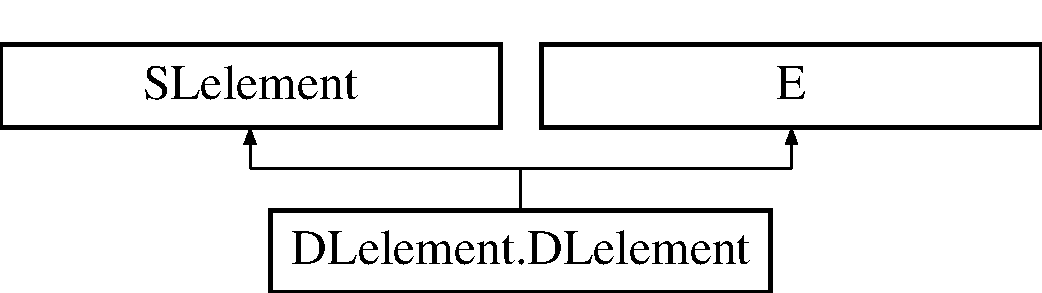
\includegraphics[height=5.000000cm]{class_d_lelement_1_1_d_lelement}
\end{center}
\end{figure}
\subsection*{Public Member Functions}
\begin{DoxyCompactItemize}
\item 
def \hyperlink{class_d_lelement_1_1_d_lelement_a37c6c1e1d648f1b8ebf44fe78e123b14}{\+\_\+\+\_\+init\+\_\+\+\_\+}
\begin{DoxyCompactList}\small\item\em Constructs an empty \hyperlink{class_d_lelement_1_1_d_lelement}{D\+Lelement} with next and prev pointers set to null. \end{DoxyCompactList}\item 
def \hyperlink{class_d_lelement_1_1_d_lelement_a9619e5ea68979dcfcc2c40e774d499d3}{get\+\_\+data\+\_\+structure\+\_\+type} (self)
\begin{DoxyCompactList}\small\item\em This method gets the data structure type. \end{DoxyCompactList}\item 
def \hyperlink{class_d_lelement_1_1_d_lelement_abd2d460265d1d725e28f761c1c400ad3}{get\+\_\+next} (self)
\begin{DoxyCompactList}\small\item\em This method returns the pointer to the next \hyperlink{class_d_lelement_1_1_d_lelement}{D\+Lelement}. \end{DoxyCompactList}\item 
def \hyperlink{class_d_lelement_1_1_d_lelement_a6c19acc6eb47b67862562fbc377a34f3}{get\+\_\+prev} (self)
\begin{DoxyCompactList}\small\item\em This method sets the pointer to the next \hyperlink{class_d_lelement_1_1_d_lelement}{D\+Lelement}. \end{DoxyCompactList}\item 
def \hyperlink{class_d_lelement_1_1_d_lelement_a8bd21c2b836357ef4b0f25444247f1e3}{set\+\_\+prev} (self, prv)
\begin{DoxyCompactList}\small\item\em This method sets the pointer to the previous \hyperlink{class_d_lelement_1_1_d_lelement}{D\+Lelement}. \end{DoxyCompactList}\item 
def \hyperlink{class_d_lelement_1_1_d_lelement_a2767441ba9442e88b64ba3c6a18adc8c}{get\+\_\+data\+\_\+structure\+\_\+representation} (self)
\begin{DoxyCompactList}\small\item\em Get the J\+S\+O\+N representation of the the data structure. \end{DoxyCompactList}\end{DoxyCompactItemize}
\subsection*{Public Attributes}
\begin{DoxyCompactItemize}
\item 
\hyperlink{class_d_lelement_1_1_d_lelement_a14bf836d9e64de3f407da9bb7ba93622}{prev}
\end{DoxyCompactItemize}
\subsection*{Static Public Attributes}
\begin{DoxyCompactItemize}
\item 
tuple \hyperlink{class_d_lelement_1_1_d_lelement_afc081f21482fb230610ba211d07abe18}{prev} = object()
\end{DoxyCompactItemize}


\subsection{Detailed Description}
This class is used to create doubly linked element objects. 

\begin{DoxyAuthor}{Author}
Mihai Mehedint, Kalpathi Subramanian
\end{DoxyAuthor}
\begin{DoxyDate}{Date}
6/22/16, 1/7/17, 5/17/17
\end{DoxyDate}
This class extends \hyperlink{namespace_element}{Element} and takes a generic parameter $<$\+E$>$ representing application specific data. This element forms the basic building block for doubly linked lists. Doubly linked elements have two links, \char`\"{}next\char`\"{} and \char`\"{}previous\char`\"{}, that point to the previous and succeeding nodes along the list.

Elements contain a visualizer (\hyperlink{namespace_element_visualizer}{Element\+Visualizer}) object for setting visual attributes (color, shape, opacity, size), necessary for displaying them in a web browser.

Elements also have a \hyperlink{namespace_link_visualizer}{Link\+Visualizer} object that is used when they are linked to another element, appropriate for setting link attributes, such as in linked lists, between the current element and its next or previous nodes.


\begin{DoxyParams}{Parameters}
{\em $<$\+E$>$} & The generic parameter object that is part of this element, representing application specific data.\\
\hline
\end{DoxyParams}
\begin{DoxySeeAlso}{See also}
Example Tutorial at ~\newline
 \href{http://bridgesuncc.github.io/Hello_World_Tutorials/DLL.html}{\tt http\+://bridgesuncc.\+github.\+io/\+Hello\+\_\+\+World\+\_\+\+Tutorials/\+D\+L\+L.\+html} 
\end{DoxySeeAlso}


\subsection{Constructor \& Destructor Documentation}
\hypertarget{class_d_lelement_1_1_d_lelement_a37c6c1e1d648f1b8ebf44fe78e123b14}{}\index{D\+Lelement\+::\+D\+Lelement@{D\+Lelement\+::\+D\+Lelement}!\+\_\+\+\_\+init\+\_\+\+\_\+@{\+\_\+\+\_\+init\+\_\+\+\_\+}}
\index{\+\_\+\+\_\+init\+\_\+\+\_\+@{\+\_\+\+\_\+init\+\_\+\+\_\+}!D\+Lelement\+::\+D\+Lelement@{D\+Lelement\+::\+D\+Lelement}}
\subsubsection[{\+\_\+\+\_\+init\+\_\+\+\_\+}]{\setlength{\rightskip}{0pt plus 5cm}def D\+Lelement.\+D\+Lelement.\+\_\+\+\_\+init\+\_\+\+\_\+ (
\begin{DoxyParamCaption}
\item[{}]{self, }
\item[{}]{e = {\ttfamily None}, }
\item[{}]{label = {\ttfamily None}, }
\item[{}]{next = {\ttfamily None}, }
\item[{}]{prev = {\ttfamily None}}
\end{DoxyParamCaption}
)}\label{class_d_lelement_1_1_d_lelement_a37c6c1e1d648f1b8ebf44fe78e123b14}


Constructs an empty \hyperlink{class_d_lelement_1_1_d_lelement}{D\+Lelement} with next and prev pointers set to null. 



\subsection{Member Function Documentation}
\hypertarget{class_d_lelement_1_1_d_lelement_a2767441ba9442e88b64ba3c6a18adc8c}{}\index{D\+Lelement\+::\+D\+Lelement@{D\+Lelement\+::\+D\+Lelement}!get\+\_\+data\+\_\+structure\+\_\+representation@{get\+\_\+data\+\_\+structure\+\_\+representation}}
\index{get\+\_\+data\+\_\+structure\+\_\+representation@{get\+\_\+data\+\_\+structure\+\_\+representation}!D\+Lelement\+::\+D\+Lelement@{D\+Lelement\+::\+D\+Lelement}}
\subsubsection[{get\+\_\+data\+\_\+structure\+\_\+representation(self)}]{\setlength{\rightskip}{0pt plus 5cm}def D\+Lelement.\+D\+Lelement.\+get\+\_\+data\+\_\+structure\+\_\+representation (
\begin{DoxyParamCaption}
\item[{}]{self}
\end{DoxyParamCaption}
)}\label{class_d_lelement_1_1_d_lelement_a2767441ba9442e88b64ba3c6a18adc8c}


Get the J\+S\+O\+N representation of the the data structure. 

\hypertarget{class_d_lelement_1_1_d_lelement_a9619e5ea68979dcfcc2c40e774d499d3}{}\index{D\+Lelement\+::\+D\+Lelement@{D\+Lelement\+::\+D\+Lelement}!get\+\_\+data\+\_\+structure\+\_\+type@{get\+\_\+data\+\_\+structure\+\_\+type}}
\index{get\+\_\+data\+\_\+structure\+\_\+type@{get\+\_\+data\+\_\+structure\+\_\+type}!D\+Lelement\+::\+D\+Lelement@{D\+Lelement\+::\+D\+Lelement}}
\subsubsection[{get\+\_\+data\+\_\+structure\+\_\+type(self)}]{\setlength{\rightskip}{0pt plus 5cm}def D\+Lelement.\+D\+Lelement.\+get\+\_\+data\+\_\+structure\+\_\+type (
\begin{DoxyParamCaption}
\item[{}]{self}
\end{DoxyParamCaption}
)}\label{class_d_lelement_1_1_d_lelement_a9619e5ea68979dcfcc2c40e774d499d3}


This method gets the data structure type. 

\begin{DoxyReturn}{Returns}
The date structure type as a string 
\end{DoxyReturn}
\hypertarget{class_d_lelement_1_1_d_lelement_abd2d460265d1d725e28f761c1c400ad3}{}\index{D\+Lelement\+::\+D\+Lelement@{D\+Lelement\+::\+D\+Lelement}!get\+\_\+next@{get\+\_\+next}}
\index{get\+\_\+next@{get\+\_\+next}!D\+Lelement\+::\+D\+Lelement@{D\+Lelement\+::\+D\+Lelement}}
\subsubsection[{get\+\_\+next(self)}]{\setlength{\rightskip}{0pt plus 5cm}def D\+Lelement.\+D\+Lelement.\+get\+\_\+next (
\begin{DoxyParamCaption}
\item[{}]{self}
\end{DoxyParamCaption}
)}\label{class_d_lelement_1_1_d_lelement_abd2d460265d1d725e28f761c1c400ad3}


This method returns the pointer to the next \hyperlink{class_d_lelement_1_1_d_lelement}{D\+Lelement}. 

\begin{DoxyReturn}{Returns}
the \hyperlink{class_d_lelement_1_1_d_lelement}{D\+Lelement} assigned to the next pointer 
\end{DoxyReturn}
\hypertarget{class_d_lelement_1_1_d_lelement_a6c19acc6eb47b67862562fbc377a34f3}{}\index{D\+Lelement\+::\+D\+Lelement@{D\+Lelement\+::\+D\+Lelement}!get\+\_\+prev@{get\+\_\+prev}}
\index{get\+\_\+prev@{get\+\_\+prev}!D\+Lelement\+::\+D\+Lelement@{D\+Lelement\+::\+D\+Lelement}}
\subsubsection[{get\+\_\+prev(self)}]{\setlength{\rightskip}{0pt plus 5cm}def D\+Lelement.\+D\+Lelement.\+get\+\_\+prev (
\begin{DoxyParamCaption}
\item[{}]{self}
\end{DoxyParamCaption}
)}\label{class_d_lelement_1_1_d_lelement_a6c19acc6eb47b67862562fbc377a34f3}


This method sets the pointer to the next \hyperlink{class_d_lelement_1_1_d_lelement}{D\+Lelement}. 


\begin{DoxyParams}{Parameters}
{\em next} & the \hyperlink{class_d_lelement_1_1_d_lelement}{D\+Lelement} that should be assigned to the next pointer\\
\hline
\end{DoxyParams}
\begin{DoxyVerb}    public void setNext(DLelement<E> nxt) {
        this.next = nxt;
        if (nxt != null)
            this.setLinkVisualizer(nxt);
    }
\end{DoxyVerb}


This method returns the pointer to the previous \hyperlink{class_d_lelement_1_1_d_lelement}{D\+Lelement}

\begin{DoxyReturn}{Returns}
the \hyperlink{class_d_lelement_1_1_d_lelement}{D\+Lelement} assigned to the prev pointer 
\end{DoxyReturn}
\hypertarget{class_d_lelement_1_1_d_lelement_a8bd21c2b836357ef4b0f25444247f1e3}{}\index{D\+Lelement\+::\+D\+Lelement@{D\+Lelement\+::\+D\+Lelement}!set\+\_\+prev@{set\+\_\+prev}}
\index{set\+\_\+prev@{set\+\_\+prev}!D\+Lelement\+::\+D\+Lelement@{D\+Lelement\+::\+D\+Lelement}}
\subsubsection[{set\+\_\+prev(self, prv)}]{\setlength{\rightskip}{0pt plus 5cm}def D\+Lelement.\+D\+Lelement.\+set\+\_\+prev (
\begin{DoxyParamCaption}
\item[{}]{self, }
\item[{}]{prv}
\end{DoxyParamCaption}
)}\label{class_d_lelement_1_1_d_lelement_a8bd21c2b836357ef4b0f25444247f1e3}


This method sets the pointer to the previous \hyperlink{class_d_lelement_1_1_d_lelement}{D\+Lelement}. 


\begin{DoxyParams}{Parameters}
{\em prev} & the \hyperlink{class_d_lelement_1_1_d_lelement}{D\+Lelement} that should be assigned to the prev pointer \\
\hline
\end{DoxyParams}


\subsection{Member Data Documentation}
\hypertarget{class_d_lelement_1_1_d_lelement_afc081f21482fb230610ba211d07abe18}{}\index{D\+Lelement\+::\+D\+Lelement@{D\+Lelement\+::\+D\+Lelement}!prev@{prev}}
\index{prev@{prev}!D\+Lelement\+::\+D\+Lelement@{D\+Lelement\+::\+D\+Lelement}}
\subsubsection[{prev}]{\setlength{\rightskip}{0pt plus 5cm}tuple D\+Lelement.\+D\+Lelement.\+prev = object()\hspace{0.3cm}{\ttfamily [static]}}\label{class_d_lelement_1_1_d_lelement_afc081f21482fb230610ba211d07abe18}
\hypertarget{class_d_lelement_1_1_d_lelement_a14bf836d9e64de3f407da9bb7ba93622}{}\index{D\+Lelement\+::\+D\+Lelement@{D\+Lelement\+::\+D\+Lelement}!prev@{prev}}
\index{prev@{prev}!D\+Lelement\+::\+D\+Lelement@{D\+Lelement\+::\+D\+Lelement}}
\subsubsection[{prev}]{\setlength{\rightskip}{0pt plus 5cm}D\+Lelement.\+D\+Lelement.\+prev}\label{class_d_lelement_1_1_d_lelement_a14bf836d9e64de3f407da9bb7ba93622}


The documentation for this class was generated from the following file\+:\begin{DoxyCompactItemize}
\item 
/\+Users/krs/gr/bridges/bridges17/python/src/\hyperlink{_d_lelement_8py}{D\+Lelement.\+py}\end{DoxyCompactItemize}

\hypertarget{class_earthquake_u_s_g_s_1_1_earthquake_u_s_g_s}{}\section{Earthquake\+U\+S\+G\+S.\+Earthquake\+U\+S\+G\+S Class Reference}
\label{class_earthquake_u_s_g_s_1_1_earthquake_u_s_g_s}\index{Earthquake\+U\+S\+G\+S.\+Earthquake\+U\+S\+G\+S@{Earthquake\+U\+S\+G\+S.\+Earthquake\+U\+S\+G\+S}}
\subsection*{Public Member Functions}
\begin{DoxyCompactItemize}
\item 
def \hyperlink{class_earthquake_u_s_g_s_1_1_earthquake_u_s_g_s_a9d4837cf374408c1dea7af8faba509f5}{get\+Date} (self)
\item 
def \hyperlink{class_earthquake_u_s_g_s_1_1_earthquake_u_s_g_s_afbfb7d79fb8873923f7f808f24f05cf4}{\+\_\+\+\_\+init\+\_\+\+\_\+}
\item 
def \hyperlink{class_earthquake_u_s_g_s_1_1_earthquake_u_s_g_s_a9ae4ad7e8b2da01287389ca0b2501c49}{get\+Time} (self)
\item 
def \hyperlink{class_earthquake_u_s_g_s_1_1_earthquake_u_s_g_s_af07aac7ca49d3d0c6a827977a57b686b}{set\+Time} (self, tm)
\item 
def \hyperlink{class_earthquake_u_s_g_s_1_1_earthquake_u_s_g_s_abaeb5aa269fc898effe87ec9924e97c5}{get\+Year} (self)
\item 
def \hyperlink{class_earthquake_u_s_g_s_1_1_earthquake_u_s_g_s_a7405c1e6bbbe7774ce9c11c6719d77cb}{get\+Month} (self)
\item 
def \hyperlink{class_earthquake_u_s_g_s_1_1_earthquake_u_s_g_s_a852a0b583bc355277761f1e5ee85dc6a}{get\+Day} (self)
\item 
def \hyperlink{class_earthquake_u_s_g_s_1_1_earthquake_u_s_g_s_ad38db7b1a922f888c23c02b7a64be7e2}{get\+Hour} (self)
\item 
def \hyperlink{class_earthquake_u_s_g_s_1_1_earthquake_u_s_g_s_a271246dee3eeb6096fc8b318e80878ee}{get\+Minutes} (self)
\item 
def \hyperlink{class_earthquake_u_s_g_s_1_1_earthquake_u_s_g_s_a7acf38ebb14eaf196a0617ba4403b4f6}{get\+Seconds} (self)
\item 
def \hyperlink{class_earthquake_u_s_g_s_1_1_earthquake_u_s_g_s_a4c47d4a79f996cf5c371b4417fec74b6}{get\+Latit} (self)
\item 
def \hyperlink{class_earthquake_u_s_g_s_1_1_earthquake_u_s_g_s_a55dcf35305d85d574cba541b26280368}{set\+Latit} (self, \hyperlink{class_earthquake_u_s_g_s_1_1_earthquake_u_s_g_s_ae115284d341b74a7e28e34e178216718}{latit})
\item 
def \hyperlink{class_earthquake_u_s_g_s_1_1_earthquake_u_s_g_s_a330c9bd81561d851f1b3ddf5a4d249de}{get\+Longit} (self)
\item 
def \hyperlink{class_earthquake_u_s_g_s_1_1_earthquake_u_s_g_s_a24157455ba676da19cb9c1ebf2361851}{set\+Longit} (self, \hyperlink{class_earthquake_u_s_g_s_1_1_earthquake_u_s_g_s_a4fec1e70f0aedd9d19f728aa5d316098}{longit})
\item 
def \hyperlink{class_earthquake_u_s_g_s_1_1_earthquake_u_s_g_s_a50a6cc08c8bbb827f66c3aee1785cdaf}{get\+Location} (self)
\item 
def \hyperlink{class_earthquake_u_s_g_s_1_1_earthquake_u_s_g_s_ae45f6b3bd60b3b2d98206e2e5e6bb764}{set\+Location} (self, \hyperlink{class_earthquake_u_s_g_s_1_1_earthquake_u_s_g_s_aa678a04be109b65cf91134acd16d95b2}{location})
\item 
def \hyperlink{class_earthquake_u_s_g_s_1_1_earthquake_u_s_g_s_a820cc015ab59c4e4a774d55a77644508}{get\+Title} (self)
\item 
def \hyperlink{class_earthquake_u_s_g_s_1_1_earthquake_u_s_g_s_aa5b4be9080eacc719731e00d00d80652}{set\+Title} (self, \hyperlink{class_earthquake_u_s_g_s_1_1_earthquake_u_s_g_s_a5ee446bf29a35b35c4e13e642c3e247a}{title})
\item 
def \hyperlink{class_earthquake_u_s_g_s_1_1_earthquake_u_s_g_s_a7bc3b1aa5b18e2bc056b913f9fcec7b3}{get\+Url} (self)
\item 
def \hyperlink{class_earthquake_u_s_g_s_1_1_earthquake_u_s_g_s_aa1b849c46667d3176566c7368208ec15}{set\+Url} (self, \hyperlink{class_earthquake_u_s_g_s_1_1_earthquake_u_s_g_s_a2636b5997fa6eeb2deb31f739a507eec}{url})
\item 
def \hyperlink{class_earthquake_u_s_g_s_1_1_earthquake_u_s_g_s_ab6db78c4e815be1642f893f84895864a}{get\+Magnitude} (self)
\item 
def \hyperlink{class_earthquake_u_s_g_s_1_1_earthquake_u_s_g_s_a54258cfad7e2adf35758f075e470f298}{set\+Magnitude} (self, \hyperlink{class_earthquake_u_s_g_s_1_1_earthquake_u_s_g_s_a8b014933b4b3373d35e20118e48d435d}{magnitude})
\end{DoxyCompactItemize}
\subsection*{Public Attributes}
\begin{DoxyCompactItemize}
\item 
\hyperlink{class_earthquake_u_s_g_s_1_1_earthquake_u_s_g_s_a8b014933b4b3373d35e20118e48d435d}{magnitude}
\item 
\hyperlink{class_earthquake_u_s_g_s_1_1_earthquake_u_s_g_s_a4fec1e70f0aedd9d19f728aa5d316098}{longit}
\item 
\hyperlink{class_earthquake_u_s_g_s_1_1_earthquake_u_s_g_s_ae115284d341b74a7e28e34e178216718}{latit}
\item 
\hyperlink{class_earthquake_u_s_g_s_1_1_earthquake_u_s_g_s_aa678a04be109b65cf91134acd16d95b2}{location}
\item 
\hyperlink{class_earthquake_u_s_g_s_1_1_earthquake_u_s_g_s_a5ee446bf29a35b35c4e13e642c3e247a}{title}
\item 
\hyperlink{class_earthquake_u_s_g_s_1_1_earthquake_u_s_g_s_a2636b5997fa6eeb2deb31f739a507eec}{url}
\item 
\hyperlink{class_earthquake_u_s_g_s_1_1_earthquake_u_s_g_s_a6273e67dccfc163a5bd72974371218a0}{time}
\item 
\hyperlink{class_earthquake_u_s_g_s_1_1_earthquake_u_s_g_s_a54d0cd00a8318c8170c39544c69353b5}{year}
\item 
\hyperlink{class_earthquake_u_s_g_s_1_1_earthquake_u_s_g_s_a3b882a16c0a432373a4f40535f913dcf}{month}
\item 
\hyperlink{class_earthquake_u_s_g_s_1_1_earthquake_u_s_g_s_afeac83440d38fc65ed1ea7a4b0e45ede}{day}
\item 
\hyperlink{class_earthquake_u_s_g_s_1_1_earthquake_u_s_g_s_ac3f8a5e9c7c811c433c15e3edff3000a}{hour}
\item 
\hyperlink{class_earthquake_u_s_g_s_1_1_earthquake_u_s_g_s_aecfe32a69e231bcd8e4e329f7d023d0e}{min}
\item 
\hyperlink{class_earthquake_u_s_g_s_1_1_earthquake_u_s_g_s_a7e81059936746568141365f9a9ccdb04}{sec}
\end{DoxyCompactItemize}


\subsection{Constructor \& Destructor Documentation}
\hypertarget{class_earthquake_u_s_g_s_1_1_earthquake_u_s_g_s_afbfb7d79fb8873923f7f808f24f05cf4}{}\index{Earthquake\+U\+S\+G\+S\+::\+Earthquake\+U\+S\+G\+S@{Earthquake\+U\+S\+G\+S\+::\+Earthquake\+U\+S\+G\+S}!\+\_\+\+\_\+init\+\_\+\+\_\+@{\+\_\+\+\_\+init\+\_\+\+\_\+}}
\index{\+\_\+\+\_\+init\+\_\+\+\_\+@{\+\_\+\+\_\+init\+\_\+\+\_\+}!Earthquake\+U\+S\+G\+S\+::\+Earthquake\+U\+S\+G\+S@{Earthquake\+U\+S\+G\+S\+::\+Earthquake\+U\+S\+G\+S}}
\subsubsection[{\+\_\+\+\_\+init\+\_\+\+\_\+}]{\setlength{\rightskip}{0pt plus 5cm}def Earthquake\+U\+S\+G\+S.\+Earthquake\+U\+S\+G\+S.\+\_\+\+\_\+init\+\_\+\+\_\+ (
\begin{DoxyParamCaption}
\item[{}]{self, }
\item[{}]{magnitude = {\ttfamily None}, }
\item[{}]{longit = {\ttfamily None}, }
\item[{}]{latit = {\ttfamily None}, }
\item[{}]{location = {\ttfamily None}, }
\item[{}]{title = {\ttfamily None}, }
\item[{}]{url = {\ttfamily None}, }
\item[{}]{time = {\ttfamily None}}
\end{DoxyParamCaption}
)}\label{class_earthquake_u_s_g_s_1_1_earthquake_u_s_g_s_afbfb7d79fb8873923f7f808f24f05cf4}


\subsection{Member Function Documentation}
\hypertarget{class_earthquake_u_s_g_s_1_1_earthquake_u_s_g_s_a9d4837cf374408c1dea7af8faba509f5}{}\index{Earthquake\+U\+S\+G\+S\+::\+Earthquake\+U\+S\+G\+S@{Earthquake\+U\+S\+G\+S\+::\+Earthquake\+U\+S\+G\+S}!get\+Date@{get\+Date}}
\index{get\+Date@{get\+Date}!Earthquake\+U\+S\+G\+S\+::\+Earthquake\+U\+S\+G\+S@{Earthquake\+U\+S\+G\+S\+::\+Earthquake\+U\+S\+G\+S}}
\subsubsection[{get\+Date(self)}]{\setlength{\rightskip}{0pt plus 5cm}def Earthquake\+U\+S\+G\+S.\+Earthquake\+U\+S\+G\+S.\+get\+Date (
\begin{DoxyParamCaption}
\item[{}]{self}
\end{DoxyParamCaption}
)}\label{class_earthquake_u_s_g_s_1_1_earthquake_u_s_g_s_a9d4837cf374408c1dea7af8faba509f5}
\hypertarget{class_earthquake_u_s_g_s_1_1_earthquake_u_s_g_s_a852a0b583bc355277761f1e5ee85dc6a}{}\index{Earthquake\+U\+S\+G\+S\+::\+Earthquake\+U\+S\+G\+S@{Earthquake\+U\+S\+G\+S\+::\+Earthquake\+U\+S\+G\+S}!get\+Day@{get\+Day}}
\index{get\+Day@{get\+Day}!Earthquake\+U\+S\+G\+S\+::\+Earthquake\+U\+S\+G\+S@{Earthquake\+U\+S\+G\+S\+::\+Earthquake\+U\+S\+G\+S}}
\subsubsection[{get\+Day(self)}]{\setlength{\rightskip}{0pt plus 5cm}def Earthquake\+U\+S\+G\+S.\+Earthquake\+U\+S\+G\+S.\+get\+Day (
\begin{DoxyParamCaption}
\item[{}]{self}
\end{DoxyParamCaption}
)}\label{class_earthquake_u_s_g_s_1_1_earthquake_u_s_g_s_a852a0b583bc355277761f1e5ee85dc6a}
\hypertarget{class_earthquake_u_s_g_s_1_1_earthquake_u_s_g_s_ad38db7b1a922f888c23c02b7a64be7e2}{}\index{Earthquake\+U\+S\+G\+S\+::\+Earthquake\+U\+S\+G\+S@{Earthquake\+U\+S\+G\+S\+::\+Earthquake\+U\+S\+G\+S}!get\+Hour@{get\+Hour}}
\index{get\+Hour@{get\+Hour}!Earthquake\+U\+S\+G\+S\+::\+Earthquake\+U\+S\+G\+S@{Earthquake\+U\+S\+G\+S\+::\+Earthquake\+U\+S\+G\+S}}
\subsubsection[{get\+Hour(self)}]{\setlength{\rightskip}{0pt plus 5cm}def Earthquake\+U\+S\+G\+S.\+Earthquake\+U\+S\+G\+S.\+get\+Hour (
\begin{DoxyParamCaption}
\item[{}]{self}
\end{DoxyParamCaption}
)}\label{class_earthquake_u_s_g_s_1_1_earthquake_u_s_g_s_ad38db7b1a922f888c23c02b7a64be7e2}
\hypertarget{class_earthquake_u_s_g_s_1_1_earthquake_u_s_g_s_a4c47d4a79f996cf5c371b4417fec74b6}{}\index{Earthquake\+U\+S\+G\+S\+::\+Earthquake\+U\+S\+G\+S@{Earthquake\+U\+S\+G\+S\+::\+Earthquake\+U\+S\+G\+S}!get\+Latit@{get\+Latit}}
\index{get\+Latit@{get\+Latit}!Earthquake\+U\+S\+G\+S\+::\+Earthquake\+U\+S\+G\+S@{Earthquake\+U\+S\+G\+S\+::\+Earthquake\+U\+S\+G\+S}}
\subsubsection[{get\+Latit(self)}]{\setlength{\rightskip}{0pt plus 5cm}def Earthquake\+U\+S\+G\+S.\+Earthquake\+U\+S\+G\+S.\+get\+Latit (
\begin{DoxyParamCaption}
\item[{}]{self}
\end{DoxyParamCaption}
)}\label{class_earthquake_u_s_g_s_1_1_earthquake_u_s_g_s_a4c47d4a79f996cf5c371b4417fec74b6}
\hypertarget{class_earthquake_u_s_g_s_1_1_earthquake_u_s_g_s_a50a6cc08c8bbb827f66c3aee1785cdaf}{}\index{Earthquake\+U\+S\+G\+S\+::\+Earthquake\+U\+S\+G\+S@{Earthquake\+U\+S\+G\+S\+::\+Earthquake\+U\+S\+G\+S}!get\+Location@{get\+Location}}
\index{get\+Location@{get\+Location}!Earthquake\+U\+S\+G\+S\+::\+Earthquake\+U\+S\+G\+S@{Earthquake\+U\+S\+G\+S\+::\+Earthquake\+U\+S\+G\+S}}
\subsubsection[{get\+Location(self)}]{\setlength{\rightskip}{0pt plus 5cm}def Earthquake\+U\+S\+G\+S.\+Earthquake\+U\+S\+G\+S.\+get\+Location (
\begin{DoxyParamCaption}
\item[{}]{self}
\end{DoxyParamCaption}
)}\label{class_earthquake_u_s_g_s_1_1_earthquake_u_s_g_s_a50a6cc08c8bbb827f66c3aee1785cdaf}
\hypertarget{class_earthquake_u_s_g_s_1_1_earthquake_u_s_g_s_a330c9bd81561d851f1b3ddf5a4d249de}{}\index{Earthquake\+U\+S\+G\+S\+::\+Earthquake\+U\+S\+G\+S@{Earthquake\+U\+S\+G\+S\+::\+Earthquake\+U\+S\+G\+S}!get\+Longit@{get\+Longit}}
\index{get\+Longit@{get\+Longit}!Earthquake\+U\+S\+G\+S\+::\+Earthquake\+U\+S\+G\+S@{Earthquake\+U\+S\+G\+S\+::\+Earthquake\+U\+S\+G\+S}}
\subsubsection[{get\+Longit(self)}]{\setlength{\rightskip}{0pt plus 5cm}def Earthquake\+U\+S\+G\+S.\+Earthquake\+U\+S\+G\+S.\+get\+Longit (
\begin{DoxyParamCaption}
\item[{}]{self}
\end{DoxyParamCaption}
)}\label{class_earthquake_u_s_g_s_1_1_earthquake_u_s_g_s_a330c9bd81561d851f1b3ddf5a4d249de}
\hypertarget{class_earthquake_u_s_g_s_1_1_earthquake_u_s_g_s_ab6db78c4e815be1642f893f84895864a}{}\index{Earthquake\+U\+S\+G\+S\+::\+Earthquake\+U\+S\+G\+S@{Earthquake\+U\+S\+G\+S\+::\+Earthquake\+U\+S\+G\+S}!get\+Magnitude@{get\+Magnitude}}
\index{get\+Magnitude@{get\+Magnitude}!Earthquake\+U\+S\+G\+S\+::\+Earthquake\+U\+S\+G\+S@{Earthquake\+U\+S\+G\+S\+::\+Earthquake\+U\+S\+G\+S}}
\subsubsection[{get\+Magnitude(self)}]{\setlength{\rightskip}{0pt plus 5cm}def Earthquake\+U\+S\+G\+S.\+Earthquake\+U\+S\+G\+S.\+get\+Magnitude (
\begin{DoxyParamCaption}
\item[{}]{self}
\end{DoxyParamCaption}
)}\label{class_earthquake_u_s_g_s_1_1_earthquake_u_s_g_s_ab6db78c4e815be1642f893f84895864a}
\hypertarget{class_earthquake_u_s_g_s_1_1_earthquake_u_s_g_s_a271246dee3eeb6096fc8b318e80878ee}{}\index{Earthquake\+U\+S\+G\+S\+::\+Earthquake\+U\+S\+G\+S@{Earthquake\+U\+S\+G\+S\+::\+Earthquake\+U\+S\+G\+S}!get\+Minutes@{get\+Minutes}}
\index{get\+Minutes@{get\+Minutes}!Earthquake\+U\+S\+G\+S\+::\+Earthquake\+U\+S\+G\+S@{Earthquake\+U\+S\+G\+S\+::\+Earthquake\+U\+S\+G\+S}}
\subsubsection[{get\+Minutes(self)}]{\setlength{\rightskip}{0pt plus 5cm}def Earthquake\+U\+S\+G\+S.\+Earthquake\+U\+S\+G\+S.\+get\+Minutes (
\begin{DoxyParamCaption}
\item[{}]{self}
\end{DoxyParamCaption}
)}\label{class_earthquake_u_s_g_s_1_1_earthquake_u_s_g_s_a271246dee3eeb6096fc8b318e80878ee}
\hypertarget{class_earthquake_u_s_g_s_1_1_earthquake_u_s_g_s_a7405c1e6bbbe7774ce9c11c6719d77cb}{}\index{Earthquake\+U\+S\+G\+S\+::\+Earthquake\+U\+S\+G\+S@{Earthquake\+U\+S\+G\+S\+::\+Earthquake\+U\+S\+G\+S}!get\+Month@{get\+Month}}
\index{get\+Month@{get\+Month}!Earthquake\+U\+S\+G\+S\+::\+Earthquake\+U\+S\+G\+S@{Earthquake\+U\+S\+G\+S\+::\+Earthquake\+U\+S\+G\+S}}
\subsubsection[{get\+Month(self)}]{\setlength{\rightskip}{0pt plus 5cm}def Earthquake\+U\+S\+G\+S.\+Earthquake\+U\+S\+G\+S.\+get\+Month (
\begin{DoxyParamCaption}
\item[{}]{self}
\end{DoxyParamCaption}
)}\label{class_earthquake_u_s_g_s_1_1_earthquake_u_s_g_s_a7405c1e6bbbe7774ce9c11c6719d77cb}
\hypertarget{class_earthquake_u_s_g_s_1_1_earthquake_u_s_g_s_a7acf38ebb14eaf196a0617ba4403b4f6}{}\index{Earthquake\+U\+S\+G\+S\+::\+Earthquake\+U\+S\+G\+S@{Earthquake\+U\+S\+G\+S\+::\+Earthquake\+U\+S\+G\+S}!get\+Seconds@{get\+Seconds}}
\index{get\+Seconds@{get\+Seconds}!Earthquake\+U\+S\+G\+S\+::\+Earthquake\+U\+S\+G\+S@{Earthquake\+U\+S\+G\+S\+::\+Earthquake\+U\+S\+G\+S}}
\subsubsection[{get\+Seconds(self)}]{\setlength{\rightskip}{0pt plus 5cm}def Earthquake\+U\+S\+G\+S.\+Earthquake\+U\+S\+G\+S.\+get\+Seconds (
\begin{DoxyParamCaption}
\item[{}]{self}
\end{DoxyParamCaption}
)}\label{class_earthquake_u_s_g_s_1_1_earthquake_u_s_g_s_a7acf38ebb14eaf196a0617ba4403b4f6}
\hypertarget{class_earthquake_u_s_g_s_1_1_earthquake_u_s_g_s_a9ae4ad7e8b2da01287389ca0b2501c49}{}\index{Earthquake\+U\+S\+G\+S\+::\+Earthquake\+U\+S\+G\+S@{Earthquake\+U\+S\+G\+S\+::\+Earthquake\+U\+S\+G\+S}!get\+Time@{get\+Time}}
\index{get\+Time@{get\+Time}!Earthquake\+U\+S\+G\+S\+::\+Earthquake\+U\+S\+G\+S@{Earthquake\+U\+S\+G\+S\+::\+Earthquake\+U\+S\+G\+S}}
\subsubsection[{get\+Time(self)}]{\setlength{\rightskip}{0pt plus 5cm}def Earthquake\+U\+S\+G\+S.\+Earthquake\+U\+S\+G\+S.\+get\+Time (
\begin{DoxyParamCaption}
\item[{}]{self}
\end{DoxyParamCaption}
)}\label{class_earthquake_u_s_g_s_1_1_earthquake_u_s_g_s_a9ae4ad7e8b2da01287389ca0b2501c49}
\hypertarget{class_earthquake_u_s_g_s_1_1_earthquake_u_s_g_s_a820cc015ab59c4e4a774d55a77644508}{}\index{Earthquake\+U\+S\+G\+S\+::\+Earthquake\+U\+S\+G\+S@{Earthquake\+U\+S\+G\+S\+::\+Earthquake\+U\+S\+G\+S}!get\+Title@{get\+Title}}
\index{get\+Title@{get\+Title}!Earthquake\+U\+S\+G\+S\+::\+Earthquake\+U\+S\+G\+S@{Earthquake\+U\+S\+G\+S\+::\+Earthquake\+U\+S\+G\+S}}
\subsubsection[{get\+Title(self)}]{\setlength{\rightskip}{0pt plus 5cm}def Earthquake\+U\+S\+G\+S.\+Earthquake\+U\+S\+G\+S.\+get\+Title (
\begin{DoxyParamCaption}
\item[{}]{self}
\end{DoxyParamCaption}
)}\label{class_earthquake_u_s_g_s_1_1_earthquake_u_s_g_s_a820cc015ab59c4e4a774d55a77644508}
\hypertarget{class_earthquake_u_s_g_s_1_1_earthquake_u_s_g_s_a7bc3b1aa5b18e2bc056b913f9fcec7b3}{}\index{Earthquake\+U\+S\+G\+S\+::\+Earthquake\+U\+S\+G\+S@{Earthquake\+U\+S\+G\+S\+::\+Earthquake\+U\+S\+G\+S}!get\+Url@{get\+Url}}
\index{get\+Url@{get\+Url}!Earthquake\+U\+S\+G\+S\+::\+Earthquake\+U\+S\+G\+S@{Earthquake\+U\+S\+G\+S\+::\+Earthquake\+U\+S\+G\+S}}
\subsubsection[{get\+Url(self)}]{\setlength{\rightskip}{0pt plus 5cm}def Earthquake\+U\+S\+G\+S.\+Earthquake\+U\+S\+G\+S.\+get\+Url (
\begin{DoxyParamCaption}
\item[{}]{self}
\end{DoxyParamCaption}
)}\label{class_earthquake_u_s_g_s_1_1_earthquake_u_s_g_s_a7bc3b1aa5b18e2bc056b913f9fcec7b3}
\hypertarget{class_earthquake_u_s_g_s_1_1_earthquake_u_s_g_s_abaeb5aa269fc898effe87ec9924e97c5}{}\index{Earthquake\+U\+S\+G\+S\+::\+Earthquake\+U\+S\+G\+S@{Earthquake\+U\+S\+G\+S\+::\+Earthquake\+U\+S\+G\+S}!get\+Year@{get\+Year}}
\index{get\+Year@{get\+Year}!Earthquake\+U\+S\+G\+S\+::\+Earthquake\+U\+S\+G\+S@{Earthquake\+U\+S\+G\+S\+::\+Earthquake\+U\+S\+G\+S}}
\subsubsection[{get\+Year(self)}]{\setlength{\rightskip}{0pt plus 5cm}def Earthquake\+U\+S\+G\+S.\+Earthquake\+U\+S\+G\+S.\+get\+Year (
\begin{DoxyParamCaption}
\item[{}]{self}
\end{DoxyParamCaption}
)}\label{class_earthquake_u_s_g_s_1_1_earthquake_u_s_g_s_abaeb5aa269fc898effe87ec9924e97c5}
\hypertarget{class_earthquake_u_s_g_s_1_1_earthquake_u_s_g_s_a55dcf35305d85d574cba541b26280368}{}\index{Earthquake\+U\+S\+G\+S\+::\+Earthquake\+U\+S\+G\+S@{Earthquake\+U\+S\+G\+S\+::\+Earthquake\+U\+S\+G\+S}!set\+Latit@{set\+Latit}}
\index{set\+Latit@{set\+Latit}!Earthquake\+U\+S\+G\+S\+::\+Earthquake\+U\+S\+G\+S@{Earthquake\+U\+S\+G\+S\+::\+Earthquake\+U\+S\+G\+S}}
\subsubsection[{set\+Latit(self, latit)}]{\setlength{\rightskip}{0pt plus 5cm}def Earthquake\+U\+S\+G\+S.\+Earthquake\+U\+S\+G\+S.\+set\+Latit (
\begin{DoxyParamCaption}
\item[{}]{self, }
\item[{}]{latit}
\end{DoxyParamCaption}
)}\label{class_earthquake_u_s_g_s_1_1_earthquake_u_s_g_s_a55dcf35305d85d574cba541b26280368}
\hypertarget{class_earthquake_u_s_g_s_1_1_earthquake_u_s_g_s_ae45f6b3bd60b3b2d98206e2e5e6bb764}{}\index{Earthquake\+U\+S\+G\+S\+::\+Earthquake\+U\+S\+G\+S@{Earthquake\+U\+S\+G\+S\+::\+Earthquake\+U\+S\+G\+S}!set\+Location@{set\+Location}}
\index{set\+Location@{set\+Location}!Earthquake\+U\+S\+G\+S\+::\+Earthquake\+U\+S\+G\+S@{Earthquake\+U\+S\+G\+S\+::\+Earthquake\+U\+S\+G\+S}}
\subsubsection[{set\+Location(self, location)}]{\setlength{\rightskip}{0pt plus 5cm}def Earthquake\+U\+S\+G\+S.\+Earthquake\+U\+S\+G\+S.\+set\+Location (
\begin{DoxyParamCaption}
\item[{}]{self, }
\item[{}]{location}
\end{DoxyParamCaption}
)}\label{class_earthquake_u_s_g_s_1_1_earthquake_u_s_g_s_ae45f6b3bd60b3b2d98206e2e5e6bb764}
\hypertarget{class_earthquake_u_s_g_s_1_1_earthquake_u_s_g_s_a24157455ba676da19cb9c1ebf2361851}{}\index{Earthquake\+U\+S\+G\+S\+::\+Earthquake\+U\+S\+G\+S@{Earthquake\+U\+S\+G\+S\+::\+Earthquake\+U\+S\+G\+S}!set\+Longit@{set\+Longit}}
\index{set\+Longit@{set\+Longit}!Earthquake\+U\+S\+G\+S\+::\+Earthquake\+U\+S\+G\+S@{Earthquake\+U\+S\+G\+S\+::\+Earthquake\+U\+S\+G\+S}}
\subsubsection[{set\+Longit(self, longit)}]{\setlength{\rightskip}{0pt plus 5cm}def Earthquake\+U\+S\+G\+S.\+Earthquake\+U\+S\+G\+S.\+set\+Longit (
\begin{DoxyParamCaption}
\item[{}]{self, }
\item[{}]{longit}
\end{DoxyParamCaption}
)}\label{class_earthquake_u_s_g_s_1_1_earthquake_u_s_g_s_a24157455ba676da19cb9c1ebf2361851}
\hypertarget{class_earthquake_u_s_g_s_1_1_earthquake_u_s_g_s_a54258cfad7e2adf35758f075e470f298}{}\index{Earthquake\+U\+S\+G\+S\+::\+Earthquake\+U\+S\+G\+S@{Earthquake\+U\+S\+G\+S\+::\+Earthquake\+U\+S\+G\+S}!set\+Magnitude@{set\+Magnitude}}
\index{set\+Magnitude@{set\+Magnitude}!Earthquake\+U\+S\+G\+S\+::\+Earthquake\+U\+S\+G\+S@{Earthquake\+U\+S\+G\+S\+::\+Earthquake\+U\+S\+G\+S}}
\subsubsection[{set\+Magnitude(self, magnitude)}]{\setlength{\rightskip}{0pt plus 5cm}def Earthquake\+U\+S\+G\+S.\+Earthquake\+U\+S\+G\+S.\+set\+Magnitude (
\begin{DoxyParamCaption}
\item[{}]{self, }
\item[{}]{magnitude}
\end{DoxyParamCaption}
)}\label{class_earthquake_u_s_g_s_1_1_earthquake_u_s_g_s_a54258cfad7e2adf35758f075e470f298}
\hypertarget{class_earthquake_u_s_g_s_1_1_earthquake_u_s_g_s_af07aac7ca49d3d0c6a827977a57b686b}{}\index{Earthquake\+U\+S\+G\+S\+::\+Earthquake\+U\+S\+G\+S@{Earthquake\+U\+S\+G\+S\+::\+Earthquake\+U\+S\+G\+S}!set\+Time@{set\+Time}}
\index{set\+Time@{set\+Time}!Earthquake\+U\+S\+G\+S\+::\+Earthquake\+U\+S\+G\+S@{Earthquake\+U\+S\+G\+S\+::\+Earthquake\+U\+S\+G\+S}}
\subsubsection[{set\+Time(self, tm)}]{\setlength{\rightskip}{0pt plus 5cm}def Earthquake\+U\+S\+G\+S.\+Earthquake\+U\+S\+G\+S.\+set\+Time (
\begin{DoxyParamCaption}
\item[{}]{self, }
\item[{}]{tm}
\end{DoxyParamCaption}
)}\label{class_earthquake_u_s_g_s_1_1_earthquake_u_s_g_s_af07aac7ca49d3d0c6a827977a57b686b}
\hypertarget{class_earthquake_u_s_g_s_1_1_earthquake_u_s_g_s_aa5b4be9080eacc719731e00d00d80652}{}\index{Earthquake\+U\+S\+G\+S\+::\+Earthquake\+U\+S\+G\+S@{Earthquake\+U\+S\+G\+S\+::\+Earthquake\+U\+S\+G\+S}!set\+Title@{set\+Title}}
\index{set\+Title@{set\+Title}!Earthquake\+U\+S\+G\+S\+::\+Earthquake\+U\+S\+G\+S@{Earthquake\+U\+S\+G\+S\+::\+Earthquake\+U\+S\+G\+S}}
\subsubsection[{set\+Title(self, title)}]{\setlength{\rightskip}{0pt plus 5cm}def Earthquake\+U\+S\+G\+S.\+Earthquake\+U\+S\+G\+S.\+set\+Title (
\begin{DoxyParamCaption}
\item[{}]{self, }
\item[{}]{title}
\end{DoxyParamCaption}
)}\label{class_earthquake_u_s_g_s_1_1_earthquake_u_s_g_s_aa5b4be9080eacc719731e00d00d80652}
\hypertarget{class_earthquake_u_s_g_s_1_1_earthquake_u_s_g_s_aa1b849c46667d3176566c7368208ec15}{}\index{Earthquake\+U\+S\+G\+S\+::\+Earthquake\+U\+S\+G\+S@{Earthquake\+U\+S\+G\+S\+::\+Earthquake\+U\+S\+G\+S}!set\+Url@{set\+Url}}
\index{set\+Url@{set\+Url}!Earthquake\+U\+S\+G\+S\+::\+Earthquake\+U\+S\+G\+S@{Earthquake\+U\+S\+G\+S\+::\+Earthquake\+U\+S\+G\+S}}
\subsubsection[{set\+Url(self, url)}]{\setlength{\rightskip}{0pt plus 5cm}def Earthquake\+U\+S\+G\+S.\+Earthquake\+U\+S\+G\+S.\+set\+Url (
\begin{DoxyParamCaption}
\item[{}]{self, }
\item[{}]{url}
\end{DoxyParamCaption}
)}\label{class_earthquake_u_s_g_s_1_1_earthquake_u_s_g_s_aa1b849c46667d3176566c7368208ec15}


\subsection{Member Data Documentation}
\hypertarget{class_earthquake_u_s_g_s_1_1_earthquake_u_s_g_s_afeac83440d38fc65ed1ea7a4b0e45ede}{}\index{Earthquake\+U\+S\+G\+S\+::\+Earthquake\+U\+S\+G\+S@{Earthquake\+U\+S\+G\+S\+::\+Earthquake\+U\+S\+G\+S}!day@{day}}
\index{day@{day}!Earthquake\+U\+S\+G\+S\+::\+Earthquake\+U\+S\+G\+S@{Earthquake\+U\+S\+G\+S\+::\+Earthquake\+U\+S\+G\+S}}
\subsubsection[{day}]{\setlength{\rightskip}{0pt plus 5cm}Earthquake\+U\+S\+G\+S.\+Earthquake\+U\+S\+G\+S.\+day}\label{class_earthquake_u_s_g_s_1_1_earthquake_u_s_g_s_afeac83440d38fc65ed1ea7a4b0e45ede}
\hypertarget{class_earthquake_u_s_g_s_1_1_earthquake_u_s_g_s_ac3f8a5e9c7c811c433c15e3edff3000a}{}\index{Earthquake\+U\+S\+G\+S\+::\+Earthquake\+U\+S\+G\+S@{Earthquake\+U\+S\+G\+S\+::\+Earthquake\+U\+S\+G\+S}!hour@{hour}}
\index{hour@{hour}!Earthquake\+U\+S\+G\+S\+::\+Earthquake\+U\+S\+G\+S@{Earthquake\+U\+S\+G\+S\+::\+Earthquake\+U\+S\+G\+S}}
\subsubsection[{hour}]{\setlength{\rightskip}{0pt plus 5cm}Earthquake\+U\+S\+G\+S.\+Earthquake\+U\+S\+G\+S.\+hour}\label{class_earthquake_u_s_g_s_1_1_earthquake_u_s_g_s_ac3f8a5e9c7c811c433c15e3edff3000a}
\hypertarget{class_earthquake_u_s_g_s_1_1_earthquake_u_s_g_s_ae115284d341b74a7e28e34e178216718}{}\index{Earthquake\+U\+S\+G\+S\+::\+Earthquake\+U\+S\+G\+S@{Earthquake\+U\+S\+G\+S\+::\+Earthquake\+U\+S\+G\+S}!latit@{latit}}
\index{latit@{latit}!Earthquake\+U\+S\+G\+S\+::\+Earthquake\+U\+S\+G\+S@{Earthquake\+U\+S\+G\+S\+::\+Earthquake\+U\+S\+G\+S}}
\subsubsection[{latit}]{\setlength{\rightskip}{0pt plus 5cm}Earthquake\+U\+S\+G\+S.\+Earthquake\+U\+S\+G\+S.\+latit}\label{class_earthquake_u_s_g_s_1_1_earthquake_u_s_g_s_ae115284d341b74a7e28e34e178216718}
\hypertarget{class_earthquake_u_s_g_s_1_1_earthquake_u_s_g_s_aa678a04be109b65cf91134acd16d95b2}{}\index{Earthquake\+U\+S\+G\+S\+::\+Earthquake\+U\+S\+G\+S@{Earthquake\+U\+S\+G\+S\+::\+Earthquake\+U\+S\+G\+S}!location@{location}}
\index{location@{location}!Earthquake\+U\+S\+G\+S\+::\+Earthquake\+U\+S\+G\+S@{Earthquake\+U\+S\+G\+S\+::\+Earthquake\+U\+S\+G\+S}}
\subsubsection[{location}]{\setlength{\rightskip}{0pt plus 5cm}Earthquake\+U\+S\+G\+S.\+Earthquake\+U\+S\+G\+S.\+location}\label{class_earthquake_u_s_g_s_1_1_earthquake_u_s_g_s_aa678a04be109b65cf91134acd16d95b2}
\hypertarget{class_earthquake_u_s_g_s_1_1_earthquake_u_s_g_s_a4fec1e70f0aedd9d19f728aa5d316098}{}\index{Earthquake\+U\+S\+G\+S\+::\+Earthquake\+U\+S\+G\+S@{Earthquake\+U\+S\+G\+S\+::\+Earthquake\+U\+S\+G\+S}!longit@{longit}}
\index{longit@{longit}!Earthquake\+U\+S\+G\+S\+::\+Earthquake\+U\+S\+G\+S@{Earthquake\+U\+S\+G\+S\+::\+Earthquake\+U\+S\+G\+S}}
\subsubsection[{longit}]{\setlength{\rightskip}{0pt plus 5cm}Earthquake\+U\+S\+G\+S.\+Earthquake\+U\+S\+G\+S.\+longit}\label{class_earthquake_u_s_g_s_1_1_earthquake_u_s_g_s_a4fec1e70f0aedd9d19f728aa5d316098}
\hypertarget{class_earthquake_u_s_g_s_1_1_earthquake_u_s_g_s_a8b014933b4b3373d35e20118e48d435d}{}\index{Earthquake\+U\+S\+G\+S\+::\+Earthquake\+U\+S\+G\+S@{Earthquake\+U\+S\+G\+S\+::\+Earthquake\+U\+S\+G\+S}!magnitude@{magnitude}}
\index{magnitude@{magnitude}!Earthquake\+U\+S\+G\+S\+::\+Earthquake\+U\+S\+G\+S@{Earthquake\+U\+S\+G\+S\+::\+Earthquake\+U\+S\+G\+S}}
\subsubsection[{magnitude}]{\setlength{\rightskip}{0pt plus 5cm}Earthquake\+U\+S\+G\+S.\+Earthquake\+U\+S\+G\+S.\+magnitude}\label{class_earthquake_u_s_g_s_1_1_earthquake_u_s_g_s_a8b014933b4b3373d35e20118e48d435d}
\hypertarget{class_earthquake_u_s_g_s_1_1_earthquake_u_s_g_s_aecfe32a69e231bcd8e4e329f7d023d0e}{}\index{Earthquake\+U\+S\+G\+S\+::\+Earthquake\+U\+S\+G\+S@{Earthquake\+U\+S\+G\+S\+::\+Earthquake\+U\+S\+G\+S}!min@{min}}
\index{min@{min}!Earthquake\+U\+S\+G\+S\+::\+Earthquake\+U\+S\+G\+S@{Earthquake\+U\+S\+G\+S\+::\+Earthquake\+U\+S\+G\+S}}
\subsubsection[{min}]{\setlength{\rightskip}{0pt plus 5cm}Earthquake\+U\+S\+G\+S.\+Earthquake\+U\+S\+G\+S.\+min}\label{class_earthquake_u_s_g_s_1_1_earthquake_u_s_g_s_aecfe32a69e231bcd8e4e329f7d023d0e}
\hypertarget{class_earthquake_u_s_g_s_1_1_earthquake_u_s_g_s_a3b882a16c0a432373a4f40535f913dcf}{}\index{Earthquake\+U\+S\+G\+S\+::\+Earthquake\+U\+S\+G\+S@{Earthquake\+U\+S\+G\+S\+::\+Earthquake\+U\+S\+G\+S}!month@{month}}
\index{month@{month}!Earthquake\+U\+S\+G\+S\+::\+Earthquake\+U\+S\+G\+S@{Earthquake\+U\+S\+G\+S\+::\+Earthquake\+U\+S\+G\+S}}
\subsubsection[{month}]{\setlength{\rightskip}{0pt plus 5cm}Earthquake\+U\+S\+G\+S.\+Earthquake\+U\+S\+G\+S.\+month}\label{class_earthquake_u_s_g_s_1_1_earthquake_u_s_g_s_a3b882a16c0a432373a4f40535f913dcf}
\hypertarget{class_earthquake_u_s_g_s_1_1_earthquake_u_s_g_s_a7e81059936746568141365f9a9ccdb04}{}\index{Earthquake\+U\+S\+G\+S\+::\+Earthquake\+U\+S\+G\+S@{Earthquake\+U\+S\+G\+S\+::\+Earthquake\+U\+S\+G\+S}!sec@{sec}}
\index{sec@{sec}!Earthquake\+U\+S\+G\+S\+::\+Earthquake\+U\+S\+G\+S@{Earthquake\+U\+S\+G\+S\+::\+Earthquake\+U\+S\+G\+S}}
\subsubsection[{sec}]{\setlength{\rightskip}{0pt plus 5cm}Earthquake\+U\+S\+G\+S.\+Earthquake\+U\+S\+G\+S.\+sec}\label{class_earthquake_u_s_g_s_1_1_earthquake_u_s_g_s_a7e81059936746568141365f9a9ccdb04}
\hypertarget{class_earthquake_u_s_g_s_1_1_earthquake_u_s_g_s_a6273e67dccfc163a5bd72974371218a0}{}\index{Earthquake\+U\+S\+G\+S\+::\+Earthquake\+U\+S\+G\+S@{Earthquake\+U\+S\+G\+S\+::\+Earthquake\+U\+S\+G\+S}!time@{time}}
\index{time@{time}!Earthquake\+U\+S\+G\+S\+::\+Earthquake\+U\+S\+G\+S@{Earthquake\+U\+S\+G\+S\+::\+Earthquake\+U\+S\+G\+S}}
\subsubsection[{time}]{\setlength{\rightskip}{0pt plus 5cm}Earthquake\+U\+S\+G\+S.\+Earthquake\+U\+S\+G\+S.\+time}\label{class_earthquake_u_s_g_s_1_1_earthquake_u_s_g_s_a6273e67dccfc163a5bd72974371218a0}
\hypertarget{class_earthquake_u_s_g_s_1_1_earthquake_u_s_g_s_a5ee446bf29a35b35c4e13e642c3e247a}{}\index{Earthquake\+U\+S\+G\+S\+::\+Earthquake\+U\+S\+G\+S@{Earthquake\+U\+S\+G\+S\+::\+Earthquake\+U\+S\+G\+S}!title@{title}}
\index{title@{title}!Earthquake\+U\+S\+G\+S\+::\+Earthquake\+U\+S\+G\+S@{Earthquake\+U\+S\+G\+S\+::\+Earthquake\+U\+S\+G\+S}}
\subsubsection[{title}]{\setlength{\rightskip}{0pt plus 5cm}Earthquake\+U\+S\+G\+S.\+Earthquake\+U\+S\+G\+S.\+title}\label{class_earthquake_u_s_g_s_1_1_earthquake_u_s_g_s_a5ee446bf29a35b35c4e13e642c3e247a}
\hypertarget{class_earthquake_u_s_g_s_1_1_earthquake_u_s_g_s_a2636b5997fa6eeb2deb31f739a507eec}{}\index{Earthquake\+U\+S\+G\+S\+::\+Earthquake\+U\+S\+G\+S@{Earthquake\+U\+S\+G\+S\+::\+Earthquake\+U\+S\+G\+S}!url@{url}}
\index{url@{url}!Earthquake\+U\+S\+G\+S\+::\+Earthquake\+U\+S\+G\+S@{Earthquake\+U\+S\+G\+S\+::\+Earthquake\+U\+S\+G\+S}}
\subsubsection[{url}]{\setlength{\rightskip}{0pt plus 5cm}Earthquake\+U\+S\+G\+S.\+Earthquake\+U\+S\+G\+S.\+url}\label{class_earthquake_u_s_g_s_1_1_earthquake_u_s_g_s_a2636b5997fa6eeb2deb31f739a507eec}
\hypertarget{class_earthquake_u_s_g_s_1_1_earthquake_u_s_g_s_a54d0cd00a8318c8170c39544c69353b5}{}\index{Earthquake\+U\+S\+G\+S\+::\+Earthquake\+U\+S\+G\+S@{Earthquake\+U\+S\+G\+S\+::\+Earthquake\+U\+S\+G\+S}!year@{year}}
\index{year@{year}!Earthquake\+U\+S\+G\+S\+::\+Earthquake\+U\+S\+G\+S@{Earthquake\+U\+S\+G\+S\+::\+Earthquake\+U\+S\+G\+S}}
\subsubsection[{year}]{\setlength{\rightskip}{0pt plus 5cm}Earthquake\+U\+S\+G\+S.\+Earthquake\+U\+S\+G\+S.\+year}\label{class_earthquake_u_s_g_s_1_1_earthquake_u_s_g_s_a54d0cd00a8318c8170c39544c69353b5}


The documentation for this class was generated from the following file\+:\begin{DoxyCompactItemize}
\item 
/\+Users/krs/gr/bridges/bridges17/python/src/data\+\_\+src\+\_\+dependent/\hyperlink{_earthquake_u_s_g_s_8py}{Earthquake\+U\+S\+G\+S.\+py}\end{DoxyCompactItemize}

\hypertarget{class_edge_1_1_edge}{}\section{Edge.\+Edge Class Reference}
\label{class_edge_1_1_edge}\index{Edge.\+Edge@{Edge.\+Edge}}


This class is used to represent the edges in a graph and will appear as links in the B\+R\+I\+D\+G\+E\+S graph visualization.  


\subsection*{Public Member Functions}
\begin{DoxyCompactItemize}
\item 
def \hyperlink{class_edge_1_1_edge_a8852f95a1f4a541b359c0d498aeea264}{\+\_\+\+\_\+init\+\_\+\+\_\+}
\begin{DoxyCompactList}\small\item\em Constructors. \end{DoxyCompactList}\item 
def \hyperlink{class_edge_1_1_edge_a00a5bb637975a294dfabc0472ccea283}{set\+\_\+weight} (self, wt)
\begin{DoxyCompactList}\small\item\em Set edge weight to \char`\"{}wt\char`\"{}. \end{DoxyCompactList}\item 
def \hyperlink{class_edge_1_1_edge_a35a3ba198529f194a234c7aaeb1f5dce}{get\+\_\+weight} (self)
\begin{DoxyCompactList}\small\item\em Get edge weight. \end{DoxyCompactList}\item 
def \hyperlink{class_edge_1_1_edge_a8ff5ba90a5163d16d2027dc854cb912f}{set\+\_\+vertex} (self, v)
\begin{DoxyCompactList}\small\item\em Set terminating \hyperlink{namespace_element}{Element} of the edge. \end{DoxyCompactList}\item 
def \hyperlink{class_edge_1_1_edge_a5a1298a3bec02315ee7ba2c6ee931808}{get\+\_\+vertex} (self)
\begin{DoxyCompactList}\small\item\em Get identifer of the terminating \hyperlink{namespace_element}{Element} of edge. \end{DoxyCompactList}\item 
def \hyperlink{class_edge_1_1_edge_aeb4f9f2847ff4b3700d93f9fb706832d}{set\+\_\+edge} (self, wt, v)
\begin{DoxyCompactList}\small\item\em Set edge to weight of \char`\"{}wt\char`\"{} and terminating Elememt of \char`\"{}v\char`\"{}. \end{DoxyCompactList}\item 
def \hyperlink{class_edge_1_1_edge_a084efa7d8d445120d670a3885098ae5b}{set\+\_\+edge\+\_\+data} (self, data)
\begin{DoxyCompactList}\small\item\em Set \hyperlink{class_edge_1_1_edge}{Edge} data (represented as a string for now) \end{DoxyCompactList}\item 
def \hyperlink{class_edge_1_1_edge_ad8870d0b9ff7cb447b888bd17dc77cb3}{get\+\_\+edge\+\_\+data} (self)
\begin{DoxyCompactList}\small\item\em Get edge data. \end{DoxyCompactList}\item 
def \hyperlink{class_edge_1_1_edge_ab99b18da5bafa083123f36ca4004925f}{get\+\_\+edge} (self)
\begin{DoxyCompactList}\small\item\em Returns this edge. \end{DoxyCompactList}\end{DoxyCompactItemize}
\subsection*{Public Attributes}
\begin{DoxyCompactItemize}
\item 
\hyperlink{class_edge_1_1_edge_a0f1b80578fe4bafb45c269111bf9822c}{weight}
\item 
\hyperlink{class_edge_1_1_edge_a024c98580ed6649429e1996725333c7b}{vertex}
\item 
\hyperlink{class_edge_1_1_edge_a7c92348b4e8e4f5027bc2fd230e353e7}{edge\+\_\+data}
\end{DoxyCompactItemize}
\subsection*{Static Public Attributes}
\begin{DoxyCompactItemize}
\item 
tuple \hyperlink{class_edge_1_1_edge_aa7dd465d78ed2c2531e23074004d2ef5}{weight} = int()
\item 
tuple \hyperlink{class_edge_1_1_edge_a48bfb886a5de7853567bac72145f61a2}{vertex} = \hyperlink{class_element_1_1_element}{Element}()
\item 
tuple \hyperlink{class_edge_1_1_edge_a97ac8ede06a4e30d3cf5d3db603b73f8}{edge\+\_\+data} = str()
\end{DoxyCompactItemize}


\subsection{Detailed Description}
This class is used to represent the edges in a graph and will appear as links in the B\+R\+I\+D\+G\+E\+S graph visualization. 

This object is used in graphs and graph algorithms such as D\+F\+S, B\+F\+S and shortest path algorithms that need to visit graph edges. The adjacency list representation uses them as the generic paramter, as S\+Lelement$<$\+Edge$>$ \hyperlink{namespace_bridges}{Bridges} represents Edges as links between pairs of elements

\begin{DoxyAuthor}{Author}
K.\+R. Subramanian
\end{DoxyAuthor}

\begin{DoxyParams}{Parameters}
{\em generic} & parameter $<$\+K$>$ usually an Element$<$\+E$>$ type used to hold the terminating vertex \\
\hline
\end{DoxyParams}


\subsection{Constructor \& Destructor Documentation}
\hypertarget{class_edge_1_1_edge_a8852f95a1f4a541b359c0d498aeea264}{}\index{Edge\+::\+Edge@{Edge\+::\+Edge}!\+\_\+\+\_\+init\+\_\+\+\_\+@{\+\_\+\+\_\+init\+\_\+\+\_\+}}
\index{\+\_\+\+\_\+init\+\_\+\+\_\+@{\+\_\+\+\_\+init\+\_\+\+\_\+}!Edge\+::\+Edge@{Edge\+::\+Edge}}
\subsubsection[{\+\_\+\+\_\+init\+\_\+\+\_\+}]{\setlength{\rightskip}{0pt plus 5cm}def Edge.\+Edge.\+\_\+\+\_\+init\+\_\+\+\_\+ (
\begin{DoxyParamCaption}
\item[{}]{self, }
\item[{}]{wt = {\ttfamily None}, }
\item[{}]{v = {\ttfamily None}}
\end{DoxyParamCaption}
)}\label{class_edge_1_1_edge_a8852f95a1f4a541b359c0d498aeea264}


Constructors. 



\subsection{Member Function Documentation}
\hypertarget{class_edge_1_1_edge_ab99b18da5bafa083123f36ca4004925f}{}\index{Edge\+::\+Edge@{Edge\+::\+Edge}!get\+\_\+edge@{get\+\_\+edge}}
\index{get\+\_\+edge@{get\+\_\+edge}!Edge\+::\+Edge@{Edge\+::\+Edge}}
\subsubsection[{get\+\_\+edge(self)}]{\setlength{\rightskip}{0pt plus 5cm}def Edge.\+Edge.\+get\+\_\+edge (
\begin{DoxyParamCaption}
\item[{}]{self}
\end{DoxyParamCaption}
)}\label{class_edge_1_1_edge_ab99b18da5bafa083123f36ca4004925f}


Returns this edge. 

\hypertarget{class_edge_1_1_edge_ad8870d0b9ff7cb447b888bd17dc77cb3}{}\index{Edge\+::\+Edge@{Edge\+::\+Edge}!get\+\_\+edge\+\_\+data@{get\+\_\+edge\+\_\+data}}
\index{get\+\_\+edge\+\_\+data@{get\+\_\+edge\+\_\+data}!Edge\+::\+Edge@{Edge\+::\+Edge}}
\subsubsection[{get\+\_\+edge\+\_\+data(self)}]{\setlength{\rightskip}{0pt plus 5cm}def Edge.\+Edge.\+get\+\_\+edge\+\_\+data (
\begin{DoxyParamCaption}
\item[{}]{self}
\end{DoxyParamCaption}
)}\label{class_edge_1_1_edge_ad8870d0b9ff7cb447b888bd17dc77cb3}


Get edge data. 

\begin{DoxyReturn}{Returns}
the edge data 
\end{DoxyReturn}
\hypertarget{class_edge_1_1_edge_a5a1298a3bec02315ee7ba2c6ee931808}{}\index{Edge\+::\+Edge@{Edge\+::\+Edge}!get\+\_\+vertex@{get\+\_\+vertex}}
\index{get\+\_\+vertex@{get\+\_\+vertex}!Edge\+::\+Edge@{Edge\+::\+Edge}}
\subsubsection[{get\+\_\+vertex(self)}]{\setlength{\rightskip}{0pt plus 5cm}def Edge.\+Edge.\+get\+\_\+vertex (
\begin{DoxyParamCaption}
\item[{}]{self}
\end{DoxyParamCaption}
)}\label{class_edge_1_1_edge_a5a1298a3bec02315ee7ba2c6ee931808}


Get identifer of the terminating \hyperlink{namespace_element}{Element} of edge. 

\begin{DoxyReturn}{Returns}
the string identifier of the terminating \hyperlink{namespace_element}{Element} 
\end{DoxyReturn}
\hypertarget{class_edge_1_1_edge_a35a3ba198529f194a234c7aaeb1f5dce}{}\index{Edge\+::\+Edge@{Edge\+::\+Edge}!get\+\_\+weight@{get\+\_\+weight}}
\index{get\+\_\+weight@{get\+\_\+weight}!Edge\+::\+Edge@{Edge\+::\+Edge}}
\subsubsection[{get\+\_\+weight(self)}]{\setlength{\rightskip}{0pt plus 5cm}def Edge.\+Edge.\+get\+\_\+weight (
\begin{DoxyParamCaption}
\item[{}]{self}
\end{DoxyParamCaption}
)}\label{class_edge_1_1_edge_a35a3ba198529f194a234c7aaeb1f5dce}


Get edge weight. 

\begin{DoxyReturn}{Returns}
the weight of edge 
\end{DoxyReturn}
\hypertarget{class_edge_1_1_edge_aeb4f9f2847ff4b3700d93f9fb706832d}{}\index{Edge\+::\+Edge@{Edge\+::\+Edge}!set\+\_\+edge@{set\+\_\+edge}}
\index{set\+\_\+edge@{set\+\_\+edge}!Edge\+::\+Edge@{Edge\+::\+Edge}}
\subsubsection[{set\+\_\+edge(self, wt, v)}]{\setlength{\rightskip}{0pt plus 5cm}def Edge.\+Edge.\+set\+\_\+edge (
\begin{DoxyParamCaption}
\item[{}]{self, }
\item[{}]{wt, }
\item[{}]{v}
\end{DoxyParamCaption}
)}\label{class_edge_1_1_edge_aeb4f9f2847ff4b3700d93f9fb706832d}


Set edge to weight of \char`\"{}wt\char`\"{} and terminating Elememt of \char`\"{}v\char`\"{}. 


\begin{DoxyParams}{Parameters}
{\em wt} & edge weight \\
\hline
{\em v} & the identifier of the terminating \hyperlink{namespace_element}{Element} \\
\hline
\end{DoxyParams}
\hypertarget{class_edge_1_1_edge_a084efa7d8d445120d670a3885098ae5b}{}\index{Edge\+::\+Edge@{Edge\+::\+Edge}!set\+\_\+edge\+\_\+data@{set\+\_\+edge\+\_\+data}}
\index{set\+\_\+edge\+\_\+data@{set\+\_\+edge\+\_\+data}!Edge\+::\+Edge@{Edge\+::\+Edge}}
\subsubsection[{set\+\_\+edge\+\_\+data(self, data)}]{\setlength{\rightskip}{0pt plus 5cm}def Edge.\+Edge.\+set\+\_\+edge\+\_\+data (
\begin{DoxyParamCaption}
\item[{}]{self, }
\item[{}]{data}
\end{DoxyParamCaption}
)}\label{class_edge_1_1_edge_a084efa7d8d445120d670a3885098ae5b}


Set \hyperlink{class_edge_1_1_edge}{Edge} data (represented as a string for now) 


\begin{DoxyParams}{Parameters}
{\em string} & application data \\
\hline
\end{DoxyParams}
\hypertarget{class_edge_1_1_edge_a8ff5ba90a5163d16d2027dc854cb912f}{}\index{Edge\+::\+Edge@{Edge\+::\+Edge}!set\+\_\+vertex@{set\+\_\+vertex}}
\index{set\+\_\+vertex@{set\+\_\+vertex}!Edge\+::\+Edge@{Edge\+::\+Edge}}
\subsubsection[{set\+\_\+vertex(self, v)}]{\setlength{\rightskip}{0pt plus 5cm}def Edge.\+Edge.\+set\+\_\+vertex (
\begin{DoxyParamCaption}
\item[{}]{self, }
\item[{}]{v}
\end{DoxyParamCaption}
)}\label{class_edge_1_1_edge_a8ff5ba90a5163d16d2027dc854cb912f}


Set terminating \hyperlink{namespace_element}{Element} of the edge. 


\begin{DoxyParams}{Parameters}
{\em v} & the identifier of the terminating \hyperlink{namespace_element}{Element} \\
\hline
\end{DoxyParams}
\hypertarget{class_edge_1_1_edge_a00a5bb637975a294dfabc0472ccea283}{}\index{Edge\+::\+Edge@{Edge\+::\+Edge}!set\+\_\+weight@{set\+\_\+weight}}
\index{set\+\_\+weight@{set\+\_\+weight}!Edge\+::\+Edge@{Edge\+::\+Edge}}
\subsubsection[{set\+\_\+weight(self, wt)}]{\setlength{\rightskip}{0pt plus 5cm}def Edge.\+Edge.\+set\+\_\+weight (
\begin{DoxyParamCaption}
\item[{}]{self, }
\item[{}]{wt}
\end{DoxyParamCaption}
)}\label{class_edge_1_1_edge_a00a5bb637975a294dfabc0472ccea283}


Set edge weight to \char`\"{}wt\char`\"{}. 


\begin{DoxyParams}{Parameters}
{\em wt} & -\/ graph edge weight \\
\hline
\end{DoxyParams}


\subsection{Member Data Documentation}
\hypertarget{class_edge_1_1_edge_a97ac8ede06a4e30d3cf5d3db603b73f8}{}\index{Edge\+::\+Edge@{Edge\+::\+Edge}!edge\+\_\+data@{edge\+\_\+data}}
\index{edge\+\_\+data@{edge\+\_\+data}!Edge\+::\+Edge@{Edge\+::\+Edge}}
\subsubsection[{edge\+\_\+data}]{\setlength{\rightskip}{0pt plus 5cm}tuple Edge.\+Edge.\+edge\+\_\+data = str()\hspace{0.3cm}{\ttfamily [static]}}\label{class_edge_1_1_edge_a97ac8ede06a4e30d3cf5d3db603b73f8}
\hypertarget{class_edge_1_1_edge_a7c92348b4e8e4f5027bc2fd230e353e7}{}\index{Edge\+::\+Edge@{Edge\+::\+Edge}!edge\+\_\+data@{edge\+\_\+data}}
\index{edge\+\_\+data@{edge\+\_\+data}!Edge\+::\+Edge@{Edge\+::\+Edge}}
\subsubsection[{edge\+\_\+data}]{\setlength{\rightskip}{0pt plus 5cm}Edge.\+Edge.\+edge\+\_\+data}\label{class_edge_1_1_edge_a7c92348b4e8e4f5027bc2fd230e353e7}
\hypertarget{class_edge_1_1_edge_a48bfb886a5de7853567bac72145f61a2}{}\index{Edge\+::\+Edge@{Edge\+::\+Edge}!vertex@{vertex}}
\index{vertex@{vertex}!Edge\+::\+Edge@{Edge\+::\+Edge}}
\subsubsection[{vertex}]{\setlength{\rightskip}{0pt plus 5cm}tuple Edge.\+Edge.\+vertex = {\bf Element}()\hspace{0.3cm}{\ttfamily [static]}}\label{class_edge_1_1_edge_a48bfb886a5de7853567bac72145f61a2}
\hypertarget{class_edge_1_1_edge_a024c98580ed6649429e1996725333c7b}{}\index{Edge\+::\+Edge@{Edge\+::\+Edge}!vertex@{vertex}}
\index{vertex@{vertex}!Edge\+::\+Edge@{Edge\+::\+Edge}}
\subsubsection[{vertex}]{\setlength{\rightskip}{0pt plus 5cm}Edge.\+Edge.\+vertex}\label{class_edge_1_1_edge_a024c98580ed6649429e1996725333c7b}
\hypertarget{class_edge_1_1_edge_aa7dd465d78ed2c2531e23074004d2ef5}{}\index{Edge\+::\+Edge@{Edge\+::\+Edge}!weight@{weight}}
\index{weight@{weight}!Edge\+::\+Edge@{Edge\+::\+Edge}}
\subsubsection[{weight}]{\setlength{\rightskip}{0pt plus 5cm}tuple Edge.\+Edge.\+weight = int()\hspace{0.3cm}{\ttfamily [static]}}\label{class_edge_1_1_edge_aa7dd465d78ed2c2531e23074004d2ef5}
\hypertarget{class_edge_1_1_edge_a0f1b80578fe4bafb45c269111bf9822c}{}\index{Edge\+::\+Edge@{Edge\+::\+Edge}!weight@{weight}}
\index{weight@{weight}!Edge\+::\+Edge@{Edge\+::\+Edge}}
\subsubsection[{weight}]{\setlength{\rightskip}{0pt plus 5cm}Edge.\+Edge.\+weight}\label{class_edge_1_1_edge_a0f1b80578fe4bafb45c269111bf9822c}


The documentation for this class was generated from the following file\+:\begin{DoxyCompactItemize}
\item 
/\+Users/krs/gr/bridges/bridges17/python/src/\hyperlink{_edge_8py}{Edge.\+py}\end{DoxyCompactItemize}

\hypertarget{class_element_1_1_element}{}\section{Element.\+Element Class Reference}
\label{class_element_1_1_element}\index{Element.\+Element@{Element.\+Element}}


This is the main superclass in B\+R\+I\+D\+G\+ES for deriving a number of objects used in building arrays, lists, trees and graph data structures.  


Inheritance diagram for Element.\+Element\+:\begin{figure}[H]
\begin{center}
\leavevmode
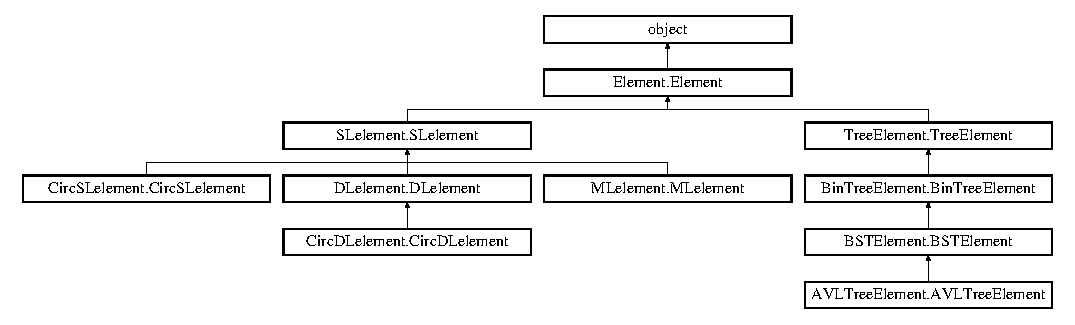
\includegraphics[height=2.000000cm]{class_element_1_1_element}
\end{center}
\end{figure}
\subsection*{Public Member Functions}
\begin{DoxyCompactItemize}
\item 
def \hyperlink{class_element_1_1_element_ad731077bce6c6caede6bdb6609672f68}{get\+Data\+Struct\+Type} (self)
\item 
def \hyperlink{class_element_1_1_element_a977b7da08b2c2ffb8d2f0c90e1fee284}{\+\_\+\+\_\+init\+\_\+\+\_\+} (self)
\begin{DoxyCompactList}\small\item\em \hyperlink{class_element_1_1_element}{Element} constructor creates an \hyperlink{namespace_element_visualizer}{Element\+Visualizer} object sets a unique identifier for the current \hyperlink{class_element_1_1_element}{Element} normally used from subclasses. \end{DoxyCompactList}\item 
def \hyperlink{class_element_1_1_element_aac5918af79bb6bd95cf429d1a219901e}{get\+Identifier} (self)
\begin{DoxyCompactList}\small\item\em this method returns the element\textquotesingle{}s unique identifier \end{DoxyCompactList}\item 
def \hyperlink{class_element_1_1_element_a83844b6ce0a822dfb09b4cdd16691ac5}{get\+Visualizer} (self)
\begin{DoxyCompactList}\small\item\em Returns the \hyperlink{class_element_1_1_element}{Element}\textquotesingle{}s visualizer object. \end{DoxyCompactList}\item 
def \hyperlink{class_element_1_1_element_a79f1e429c47e65341273e9971ff1ece0}{set\+Visualizer} (self, \hyperlink{class_element_1_1_element_a7a5b8e1891bf065fa81f51a8f6b4212e}{visualizer})
\begin{DoxyCompactList}\small\item\em This method sets the visualizer object for the current element object. \end{DoxyCompactList}\item 
def \hyperlink{class_element_1_1_element_aad4a71d78f6c60de5bf871fd7632d720}{get\+Link\+Visualizer} (self, el)
\begin{DoxyCompactList}\small\item\em Returns the \hyperlink{class_element_1_1_element}{Element}\textquotesingle{}s link visualizer object. \end{DoxyCompactList}\item 
def \hyperlink{class_element_1_1_element_a6aac3e4778ae009406417439c778f904}{set\+Link\+Visualizer} (self, el)
\begin{DoxyCompactList}\small\item\em Sets the link from this element to a new incoming element. \end{DoxyCompactList}\item 
def \hyperlink{class_element_1_1_element_a2dde72f6339b9d052df50bb4a5de2502}{remove\+Link\+Visualizer} (self, el)
\item 
def \hyperlink{class_element_1_1_element_ae864741d8f6e980b2ecb4bed62e87e96}{validate\+Val} (self, \hyperlink{class_element_1_1_element_ae9c30f7574a4356686d93e4567cf61f8}{value})
\begin{DoxyCompactList}\small\item\em Validates the \hyperlink{class_element_1_1_element}{Element}\textquotesingle{}s value when the \hyperlink{class_element_1_1_element}{Element} is created A non null value is expected this will be unnecessary after we modify the server. \end{DoxyCompactList}\item 
def \hyperlink{class_element_1_1_element_a5e7edd71cdc182f6449cdb47fb6d396b}{get\+Class\+Name} (self)
\item 
def \hyperlink{class_element_1_1_element_acc377fb2d5856281eb9804b2a3275edc}{compare\+To} (self, e1)
\item 
def \hyperlink{class_element_1_1_element_adf032a6f79735b75e3f1071cc708f626}{equals} (self, e1)
\item 
def \hyperlink{class_element_1_1_element_a5fa599166de5a0053b235d012fbfc42c}{get\+Element\+Representation} (self)
\item 
def \hyperlink{class_element_1_1_element_a87e09915bdcd4d07efb293d54ca5b270}{get\+Link\+Representation} (self, lv, src, dest)
\item 
def \hyperlink{class_element_1_1_element_a52a3e2777d110a86950a6e88dfcdd0a4}{get\+Label} (self)
\item 
def \hyperlink{class_element_1_1_element_a21af17ef037212f8ab693ec66952e4ac}{set\+Label} (self, \hyperlink{class_element_1_1_element_a1eaadb79747dd83097612cac742976fa}{label})
\item 
def \hyperlink{class_element_1_1_element_ab68f114977f0cc57c9499444d2bc8799}{arrange\+Label} (self, \hyperlink{class_element_1_1_element_a1eaadb79747dd83097612cac742976fa}{label}, \hyperlink{class_element_1_1_element_a58cc88e7f79da391e25e4fa98845b8cc}{word\+Number})
\item 
def \hyperlink{class_element_1_1_element_a55c19f29f1c643e13e11441c4f3491e0}{get\+Value} (self)
\item 
def \hyperlink{class_element_1_1_element_a267a7f5770e823ca3b6e5bc88fa6dfa9}{set\+Value} (self, \hyperlink{class_element_1_1_element_ae9c30f7574a4356686d93e4567cf61f8}{value})
\item 
def \hyperlink{class_element_1_1_element_a2ffb262087576d15a2e93b864d4ce13a}{\+\_\+\+\_\+str\+\_\+\+\_\+} (self)
\end{DoxyCompactItemize}
\subsection*{Static Public Attributes}
\begin{DoxyCompactItemize}
\item 
int \hyperlink{class_element_1_1_element_a219a21d962bfef58ad39c9762876588f}{ids} = 0
\item 
\hyperlink{class_element_1_1_element_a1eaadb79747dd83097612cac742976fa}{label} = str()
\item 
\hyperlink{class_element_1_1_element_a2202a62a079908d52afc0b7796be2981}{identifier} = str()
\item 
\hyperlink{class_element_1_1_element_a7a5b8e1891bf065fa81f51a8f6b4212e}{visualizer} = Element\+Visualizer()
\item 
\hyperlink{class_element_1_1_element_a130630f8ecfe9255c9e0a514949be201}{lvisualizer} = Hash\+Map()
\item 
\hyperlink{class_element_1_1_element_ae9c30f7574a4356686d93e4567cf61f8}{value} = E()
\item 
int \hyperlink{class_element_1_1_element_a58cc88e7f79da391e25e4fa98845b8cc}{word\+Number} = 0
\item 
string \hyperlink{class_element_1_1_element_a346648cd57ba439d8b4913a645ab81ba}{I\+N\+S\+E\+R\+T\+\_\+\+S\+T\+R\+I\+NG} = \char`\"{}\textbackslash{}\textbackslash{}n\char`\"{}
\item 
string \hyperlink{class_element_1_1_element_ae06a0f0ca0e5499c532f2550cf1ffea6}{D\+I\+V\+I\+D\+E\+\_\+\+K\+EY} = \char`\"{}(\textbackslash{}r?\textbackslash{}n)$\vert$(\textbackslash{}n)$\vert$(\textbackslash{}f)$\vert$(\textbackslash{}r)$\vert$(\%n)\char`\"{}
\end{DoxyCompactItemize}


\subsection{Detailed Description}
This is the main superclass in B\+R\+I\+D\+G\+ES for deriving a number of objects used in building arrays, lists, trees and graph data structures. 

\hyperlink{namespace_s_lelement}{S\+Lelement}, D\+Lelement, \hyperlink{namespace_circ_s_lelement}{Circ\+S\+Lelement}, \hyperlink{namespace_circ_d_lelement}{Circ\+D\+Lelement}, Tree\+Element, \hyperlink{namespace_bin_tree_element}{Bin\+Tree\+Element}, B\+S\+T\+Element, \hyperlink{namespace_circ_s_lelement}{Circ\+S\+Lelement}, \hyperlink{namespace_circ_d_lelement}{Circ\+D\+Lelement}, \hyperlink{namespace_a_v_l_tree_element}{A\+V\+L\+Tree\+Element} are all subclasses (see class hierarchy above). \hyperlink{class_element_1_1_element}{Element} contains two visualizer objects (\hyperlink{namespace_element_visualizer}{Element\+Visualizer}, \hyperlink{namespace_link_visualizer}{Link\+Visualizer}) for specifying visual attributes for nodes and links respectively. It also contains a label that that can be displayed in B\+R\+I\+D\+G\+ES visualizations.

All the tutorials under

\href{http://bridgesuncc.github.io/Hello_World_Tutorials/Overview.html}{\tt http\+://bridgesuncc.\+github.\+io/\+Hello\+\_\+\+World\+\_\+\+Tutorials/\+Overview.\+html}

illustrate examples of using different types of \hyperlink{class_element_1_1_element}{Element} objects and how to manipulate their visual attributes.

\begin{DoxyAuthor}{Author}
Mihai Mehedint, Kalpathi Subramanian
\end{DoxyAuthor}

\begin{DoxyParams}{Parameters}
{\em generic} & $<$\+E$>$ Elements are defined with an application specific generic parameter, that is defined by the user. These can be any legal Java type and manipulated using \hyperlink{class_element_1_1_element_a267a7f5770e823ca3b6e5bc88fa6dfa9}{set\+Value()}/get\+Value() methods. For more information on Java generics, see for example, \href{https://docs.oracle.com/javase/tutorial/java/generics/types.html@verbatim}{\tt https\+://docs.\+oracle.\+com/javase/tutorial/java/generics/types.\+html@verbatim} generated source for class \hyperlink{class_element_1_1_element}{Element}  \\
\hline
\end{DoxyParams}


\subsection{Constructor \& Destructor Documentation}
\hypertarget{class_element_1_1_element_a977b7da08b2c2ffb8d2f0c90e1fee284}{}\label{class_element_1_1_element_a977b7da08b2c2ffb8d2f0c90e1fee284} 
\index{Element\+::\+Element@{Element\+::\+Element}!\+\_\+\+\_\+init\+\_\+\+\_\+@{\+\_\+\+\_\+init\+\_\+\+\_\+}}
\index{\+\_\+\+\_\+init\+\_\+\+\_\+@{\+\_\+\+\_\+init\+\_\+\+\_\+}!Element\+::\+Element@{Element\+::\+Element}}
\subsubsection{\texorpdfstring{\+\_\+\+\_\+init\+\_\+\+\_\+()}{\_\_init\_\_()}}
{\footnotesize\ttfamily def Element.\+Element.\+\_\+\+\_\+init\+\_\+\+\_\+ (\begin{DoxyParamCaption}\item[{}]{self }\end{DoxyParamCaption})}



\hyperlink{class_element_1_1_element}{Element} constructor creates an \hyperlink{namespace_element_visualizer}{Element\+Visualizer} object sets a unique identifier for the current \hyperlink{class_element_1_1_element}{Element} normally used from subclasses. 

\begin{DoxyVerb}generated source for method __init__ \end{DoxyVerb}
 

\subsection{Member Function Documentation}
\hypertarget{class_element_1_1_element_a2ffb262087576d15a2e93b864d4ce13a}{}\label{class_element_1_1_element_a2ffb262087576d15a2e93b864d4ce13a} 
\index{Element\+::\+Element@{Element\+::\+Element}!\+\_\+\+\_\+str\+\_\+\+\_\+@{\+\_\+\+\_\+str\+\_\+\+\_\+}}
\index{\+\_\+\+\_\+str\+\_\+\+\_\+@{\+\_\+\+\_\+str\+\_\+\+\_\+}!Element\+::\+Element@{Element\+::\+Element}}
\subsubsection{\texorpdfstring{\+\_\+\+\_\+str\+\_\+\+\_\+()}{\_\_str\_\_()}}
{\footnotesize\ttfamily def Element.\+Element.\+\_\+\+\_\+str\+\_\+\+\_\+ (\begin{DoxyParamCaption}\item[{}]{self }\end{DoxyParamCaption})}

\begin{DoxyVerb}generated source for method toString \end{DoxyVerb}
 \hypertarget{class_element_1_1_element_ab68f114977f0cc57c9499444d2bc8799}{}\label{class_element_1_1_element_ab68f114977f0cc57c9499444d2bc8799} 
\index{Element\+::\+Element@{Element\+::\+Element}!arrange\+Label@{arrange\+Label}}
\index{arrange\+Label@{arrange\+Label}!Element\+::\+Element@{Element\+::\+Element}}
\subsubsection{\texorpdfstring{arrange\+Label()}{arrangeLabel()}}
{\footnotesize\ttfamily def Element.\+Element.\+arrange\+Label (\begin{DoxyParamCaption}\item[{}]{self,  }\item[{}]{label,  }\item[{}]{word\+Number }\end{DoxyParamCaption})}

\begin{DoxyVerb}generated source for method arrangeLabel \end{DoxyVerb}
 \hypertarget{class_element_1_1_element_acc377fb2d5856281eb9804b2a3275edc}{}\label{class_element_1_1_element_acc377fb2d5856281eb9804b2a3275edc} 
\index{Element\+::\+Element@{Element\+::\+Element}!compare\+To@{compare\+To}}
\index{compare\+To@{compare\+To}!Element\+::\+Element@{Element\+::\+Element}}
\subsubsection{\texorpdfstring{compare\+To()}{compareTo()}}
{\footnotesize\ttfamily def Element.\+Element.\+compare\+To (\begin{DoxyParamCaption}\item[{}]{self,  }\item[{}]{e1 }\end{DoxyParamCaption})}

\begin{DoxyVerb}generated source for method compareTo \end{DoxyVerb}
 \hypertarget{class_element_1_1_element_adf032a6f79735b75e3f1071cc708f626}{}\label{class_element_1_1_element_adf032a6f79735b75e3f1071cc708f626} 
\index{Element\+::\+Element@{Element\+::\+Element}!equals@{equals}}
\index{equals@{equals}!Element\+::\+Element@{Element\+::\+Element}}
\subsubsection{\texorpdfstring{equals()}{equals()}}
{\footnotesize\ttfamily def Element.\+Element.\+equals (\begin{DoxyParamCaption}\item[{}]{self,  }\item[{}]{e1 }\end{DoxyParamCaption})}

\begin{DoxyVerb}generated source for method equals \end{DoxyVerb}
 \hypertarget{class_element_1_1_element_a5e7edd71cdc182f6449cdb47fb6d396b}{}\label{class_element_1_1_element_a5e7edd71cdc182f6449cdb47fb6d396b} 
\index{Element\+::\+Element@{Element\+::\+Element}!get\+Class\+Name@{get\+Class\+Name}}
\index{get\+Class\+Name@{get\+Class\+Name}!Element\+::\+Element@{Element\+::\+Element}}
\subsubsection{\texorpdfstring{get\+Class\+Name()}{getClassName()}}
{\footnotesize\ttfamily def Element.\+Element.\+get\+Class\+Name (\begin{DoxyParamCaption}\item[{}]{self }\end{DoxyParamCaption})}

\begin{DoxyVerb}generated source for method getClassName \end{DoxyVerb}
 \hypertarget{class_element_1_1_element_ad731077bce6c6caede6bdb6609672f68}{}\label{class_element_1_1_element_ad731077bce6c6caede6bdb6609672f68} 
\index{Element\+::\+Element@{Element\+::\+Element}!get\+Data\+Struct\+Type@{get\+Data\+Struct\+Type}}
\index{get\+Data\+Struct\+Type@{get\+Data\+Struct\+Type}!Element\+::\+Element@{Element\+::\+Element}}
\subsubsection{\texorpdfstring{get\+Data\+Struct\+Type()}{getDataStructType()}}
{\footnotesize\ttfamily def Element.\+Element.\+get\+Data\+Struct\+Type (\begin{DoxyParamCaption}\item[{}]{self }\end{DoxyParamCaption})}

\begin{DoxyVerb}generated source for method getDataStructType \end{DoxyVerb}
 \hypertarget{class_element_1_1_element_a5fa599166de5a0053b235d012fbfc42c}{}\label{class_element_1_1_element_a5fa599166de5a0053b235d012fbfc42c} 
\index{Element\+::\+Element@{Element\+::\+Element}!get\+Element\+Representation@{get\+Element\+Representation}}
\index{get\+Element\+Representation@{get\+Element\+Representation}!Element\+::\+Element@{Element\+::\+Element}}
\subsubsection{\texorpdfstring{get\+Element\+Representation()}{getElementRepresentation()}}
{\footnotesize\ttfamily def Element.\+Element.\+get\+Element\+Representation (\begin{DoxyParamCaption}\item[{}]{self }\end{DoxyParamCaption})}

\begin{DoxyVerb}generated source for method getElementRepresentation \end{DoxyVerb}
 \hypertarget{class_element_1_1_element_aac5918af79bb6bd95cf429d1a219901e}{}\label{class_element_1_1_element_aac5918af79bb6bd95cf429d1a219901e} 
\index{Element\+::\+Element@{Element\+::\+Element}!get\+Identifier@{get\+Identifier}}
\index{get\+Identifier@{get\+Identifier}!Element\+::\+Element@{Element\+::\+Element}}
\subsubsection{\texorpdfstring{get\+Identifier()}{getIdentifier()}}
{\footnotesize\ttfamily def Element.\+Element.\+get\+Identifier (\begin{DoxyParamCaption}\item[{}]{self }\end{DoxyParamCaption})}



this method returns the element\textquotesingle{}s unique identifier 

\begin{DoxyReturn}{Returns}
the string identifier\begin{DoxyVerb}generated source for method getIdentifier \end{DoxyVerb}
 
\end{DoxyReturn}
\hypertarget{class_element_1_1_element_a52a3e2777d110a86950a6e88dfcdd0a4}{}\label{class_element_1_1_element_a52a3e2777d110a86950a6e88dfcdd0a4} 
\index{Element\+::\+Element@{Element\+::\+Element}!get\+Label@{get\+Label}}
\index{get\+Label@{get\+Label}!Element\+::\+Element@{Element\+::\+Element}}
\subsubsection{\texorpdfstring{get\+Label()}{getLabel()}}
{\footnotesize\ttfamily def Element.\+Element.\+get\+Label (\begin{DoxyParamCaption}\item[{}]{self }\end{DoxyParamCaption})}

\begin{DoxyVerb}generated source for method getLabel \end{DoxyVerb}
 \hypertarget{class_element_1_1_element_a87e09915bdcd4d07efb293d54ca5b270}{}\label{class_element_1_1_element_a87e09915bdcd4d07efb293d54ca5b270} 
\index{Element\+::\+Element@{Element\+::\+Element}!get\+Link\+Representation@{get\+Link\+Representation}}
\index{get\+Link\+Representation@{get\+Link\+Representation}!Element\+::\+Element@{Element\+::\+Element}}
\subsubsection{\texorpdfstring{get\+Link\+Representation()}{getLinkRepresentation()}}
{\footnotesize\ttfamily def Element.\+Element.\+get\+Link\+Representation (\begin{DoxyParamCaption}\item[{}]{self,  }\item[{}]{lv,  }\item[{}]{src,  }\item[{}]{dest }\end{DoxyParamCaption})}

\begin{DoxyVerb}generated source for method getLinkRepresentation \end{DoxyVerb}
 \hypertarget{class_element_1_1_element_aad4a71d78f6c60de5bf871fd7632d720}{}\label{class_element_1_1_element_aad4a71d78f6c60de5bf871fd7632d720} 
\index{Element\+::\+Element@{Element\+::\+Element}!get\+Link\+Visualizer@{get\+Link\+Visualizer}}
\index{get\+Link\+Visualizer@{get\+Link\+Visualizer}!Element\+::\+Element@{Element\+::\+Element}}
\subsubsection{\texorpdfstring{get\+Link\+Visualizer()}{getLinkVisualizer()}}
{\footnotesize\ttfamily def Element.\+Element.\+get\+Link\+Visualizer (\begin{DoxyParamCaption}\item[{}]{self,  }\item[{}]{el }\end{DoxyParamCaption})}



Returns the \hyperlink{class_element_1_1_element}{Element}\textquotesingle{}s link visualizer object. 

The link visualizer object links this element to another element, which is specified by the argument to this method. This method is typically used to set the visual attributes of the links, such as in graphs or binary tree structures.

\hyperlink{class_element_1_1_element}{Element} el -- the element terminating the link

\begin{DoxyReturn}{Returns}
the link visualizer\begin{DoxyVerb}generated source for method getLinkVisualizer \end{DoxyVerb}
 
\end{DoxyReturn}
\hypertarget{class_element_1_1_element_a55c19f29f1c643e13e11441c4f3491e0}{}\label{class_element_1_1_element_a55c19f29f1c643e13e11441c4f3491e0} 
\index{Element\+::\+Element@{Element\+::\+Element}!get\+Value@{get\+Value}}
\index{get\+Value@{get\+Value}!Element\+::\+Element@{Element\+::\+Element}}
\subsubsection{\texorpdfstring{get\+Value()}{getValue()}}
{\footnotesize\ttfamily def Element.\+Element.\+get\+Value (\begin{DoxyParamCaption}\item[{}]{self }\end{DoxyParamCaption})}

\begin{DoxyVerb}generated source for method getValue \end{DoxyVerb}
 \hypertarget{class_element_1_1_element_a83844b6ce0a822dfb09b4cdd16691ac5}{}\label{class_element_1_1_element_a83844b6ce0a822dfb09b4cdd16691ac5} 
\index{Element\+::\+Element@{Element\+::\+Element}!get\+Visualizer@{get\+Visualizer}}
\index{get\+Visualizer@{get\+Visualizer}!Element\+::\+Element@{Element\+::\+Element}}
\subsubsection{\texorpdfstring{get\+Visualizer()}{getVisualizer()}}
{\footnotesize\ttfamily def Element.\+Element.\+get\+Visualizer (\begin{DoxyParamCaption}\item[{}]{self }\end{DoxyParamCaption})}



Returns the \hyperlink{class_element_1_1_element}{Element}\textquotesingle{}s visualizer object. 

\begin{DoxyReturn}{Returns}
the visualizer object\begin{DoxyVerb}generated source for method getVisualizer \end{DoxyVerb}
 
\end{DoxyReturn}
\hypertarget{class_element_1_1_element_a2dde72f6339b9d052df50bb4a5de2502}{}\label{class_element_1_1_element_a2dde72f6339b9d052df50bb4a5de2502} 
\index{Element\+::\+Element@{Element\+::\+Element}!remove\+Link\+Visualizer@{remove\+Link\+Visualizer}}
\index{remove\+Link\+Visualizer@{remove\+Link\+Visualizer}!Element\+::\+Element@{Element\+::\+Element}}
\subsubsection{\texorpdfstring{remove\+Link\+Visualizer()}{removeLinkVisualizer()}}
{\footnotesize\ttfamily def Element.\+Element.\+remove\+Link\+Visualizer (\begin{DoxyParamCaption}\item[{}]{self,  }\item[{}]{el }\end{DoxyParamCaption})}

\begin{DoxyVerb}generated source for method removeLinkVisualizer \end{DoxyVerb}
 \hypertarget{class_element_1_1_element_a21af17ef037212f8ab693ec66952e4ac}{}\label{class_element_1_1_element_a21af17ef037212f8ab693ec66952e4ac} 
\index{Element\+::\+Element@{Element\+::\+Element}!set\+Label@{set\+Label}}
\index{set\+Label@{set\+Label}!Element\+::\+Element@{Element\+::\+Element}}
\subsubsection{\texorpdfstring{set\+Label()}{setLabel()}}
{\footnotesize\ttfamily def Element.\+Element.\+set\+Label (\begin{DoxyParamCaption}\item[{}]{self,  }\item[{}]{label }\end{DoxyParamCaption})}

\begin{DoxyVerb}generated source for method setLabel \end{DoxyVerb}
 \hypertarget{class_element_1_1_element_a6aac3e4778ae009406417439c778f904}{}\label{class_element_1_1_element_a6aac3e4778ae009406417439c778f904} 
\index{Element\+::\+Element@{Element\+::\+Element}!set\+Link\+Visualizer@{set\+Link\+Visualizer}}
\index{set\+Link\+Visualizer@{set\+Link\+Visualizer}!Element\+::\+Element@{Element\+::\+Element}}
\subsubsection{\texorpdfstring{set\+Link\+Visualizer()}{setLinkVisualizer()}}
{\footnotesize\ttfamily def Element.\+Element.\+set\+Link\+Visualizer (\begin{DoxyParamCaption}\item[{}]{self,  }\item[{}]{el }\end{DoxyParamCaption})}



Sets the link from this element to a new incoming element. 


\begin{DoxyParams}{Parameters}
{\em el} & the element to be linked to.\begin{DoxyVerb}generated source for method setLinkVisualizer \end{DoxyVerb}
 \\
\hline
\end{DoxyParams}
\hypertarget{class_element_1_1_element_a267a7f5770e823ca3b6e5bc88fa6dfa9}{}\label{class_element_1_1_element_a267a7f5770e823ca3b6e5bc88fa6dfa9} 
\index{Element\+::\+Element@{Element\+::\+Element}!set\+Value@{set\+Value}}
\index{set\+Value@{set\+Value}!Element\+::\+Element@{Element\+::\+Element}}
\subsubsection{\texorpdfstring{set\+Value()}{setValue()}}
{\footnotesize\ttfamily def Element.\+Element.\+set\+Value (\begin{DoxyParamCaption}\item[{}]{self,  }\item[{}]{value }\end{DoxyParamCaption})}

\begin{DoxyVerb}generated source for method setValue \end{DoxyVerb}
 \hypertarget{class_element_1_1_element_a79f1e429c47e65341273e9971ff1ece0}{}\label{class_element_1_1_element_a79f1e429c47e65341273e9971ff1ece0} 
\index{Element\+::\+Element@{Element\+::\+Element}!set\+Visualizer@{set\+Visualizer}}
\index{set\+Visualizer@{set\+Visualizer}!Element\+::\+Element@{Element\+::\+Element}}
\subsubsection{\texorpdfstring{set\+Visualizer()}{setVisualizer()}}
{\footnotesize\ttfamily def Element.\+Element.\+set\+Visualizer (\begin{DoxyParamCaption}\item[{}]{self,  }\item[{}]{visualizer }\end{DoxyParamCaption})}



This method sets the visualizer object for the current element object. 


\begin{DoxyParams}{Parameters}
{\em visualizer} & the visualizer to set\begin{DoxyVerb}generated source for method setVisualizer \end{DoxyVerb}
 \\
\hline
\end{DoxyParams}
\hypertarget{class_element_1_1_element_ae864741d8f6e980b2ecb4bed62e87e96}{}\label{class_element_1_1_element_ae864741d8f6e980b2ecb4bed62e87e96} 
\index{Element\+::\+Element@{Element\+::\+Element}!validate\+Val@{validate\+Val}}
\index{validate\+Val@{validate\+Val}!Element\+::\+Element@{Element\+::\+Element}}
\subsubsection{\texorpdfstring{validate\+Val()}{validateVal()}}
{\footnotesize\ttfamily def Element.\+Element.\+validate\+Val (\begin{DoxyParamCaption}\item[{}]{self,  }\item[{}]{value }\end{DoxyParamCaption})}



Validates the \hyperlink{class_element_1_1_element}{Element}\textquotesingle{}s value when the \hyperlink{class_element_1_1_element}{Element} is created A non null value is expected this will be unnecessary after we modify the server. 


\begin{DoxyParams}{Parameters}
{\em E\+Lement} & value\begin{DoxyVerb}generated source for method validateVal \end{DoxyVerb}
 \\
\hline
\end{DoxyParams}


\subsection{Member Data Documentation}
\hypertarget{class_element_1_1_element_ae06a0f0ca0e5499c532f2550cf1ffea6}{}\label{class_element_1_1_element_ae06a0f0ca0e5499c532f2550cf1ffea6} 
\index{Element\+::\+Element@{Element\+::\+Element}!D\+I\+V\+I\+D\+E\+\_\+\+K\+EY@{D\+I\+V\+I\+D\+E\+\_\+\+K\+EY}}
\index{D\+I\+V\+I\+D\+E\+\_\+\+K\+EY@{D\+I\+V\+I\+D\+E\+\_\+\+K\+EY}!Element\+::\+Element@{Element\+::\+Element}}
\subsubsection{\texorpdfstring{D\+I\+V\+I\+D\+E\+\_\+\+K\+EY}{DIVIDE\_KEY}}
{\footnotesize\ttfamily string Element.\+Element.\+D\+I\+V\+I\+D\+E\+\_\+\+K\+EY = \char`\"{}(\textbackslash{}r?\textbackslash{}n)$\vert$(\textbackslash{}n)$\vert$(\textbackslash{}f)$\vert$(\textbackslash{}r)$\vert$(\%n)\char`\"{}\hspace{0.3cm}{\ttfamily [static]}}

\hypertarget{class_element_1_1_element_a2202a62a079908d52afc0b7796be2981}{}\label{class_element_1_1_element_a2202a62a079908d52afc0b7796be2981} 
\index{Element\+::\+Element@{Element\+::\+Element}!identifier@{identifier}}
\index{identifier@{identifier}!Element\+::\+Element@{Element\+::\+Element}}
\subsubsection{\texorpdfstring{identifier}{identifier}}
{\footnotesize\ttfamily Element.\+Element.\+identifier = str()\hspace{0.3cm}{\ttfamily [static]}}

\hypertarget{class_element_1_1_element_a219a21d962bfef58ad39c9762876588f}{}\label{class_element_1_1_element_a219a21d962bfef58ad39c9762876588f} 
\index{Element\+::\+Element@{Element\+::\+Element}!ids@{ids}}
\index{ids@{ids}!Element\+::\+Element@{Element\+::\+Element}}
\subsubsection{\texorpdfstring{ids}{ids}}
{\footnotesize\ttfamily int Element.\+Element.\+ids = 0\hspace{0.3cm}{\ttfamily [static]}}

\hypertarget{class_element_1_1_element_a346648cd57ba439d8b4913a645ab81ba}{}\label{class_element_1_1_element_a346648cd57ba439d8b4913a645ab81ba} 
\index{Element\+::\+Element@{Element\+::\+Element}!I\+N\+S\+E\+R\+T\+\_\+\+S\+T\+R\+I\+NG@{I\+N\+S\+E\+R\+T\+\_\+\+S\+T\+R\+I\+NG}}
\index{I\+N\+S\+E\+R\+T\+\_\+\+S\+T\+R\+I\+NG@{I\+N\+S\+E\+R\+T\+\_\+\+S\+T\+R\+I\+NG}!Element\+::\+Element@{Element\+::\+Element}}
\subsubsection{\texorpdfstring{I\+N\+S\+E\+R\+T\+\_\+\+S\+T\+R\+I\+NG}{INSERT\_STRING}}
{\footnotesize\ttfamily string Element.\+Element.\+I\+N\+S\+E\+R\+T\+\_\+\+S\+T\+R\+I\+NG = \char`\"{}\textbackslash{}\textbackslash{}n\char`\"{}\hspace{0.3cm}{\ttfamily [static]}}

\hypertarget{class_element_1_1_element_a1eaadb79747dd83097612cac742976fa}{}\label{class_element_1_1_element_a1eaadb79747dd83097612cac742976fa} 
\index{Element\+::\+Element@{Element\+::\+Element}!label@{label}}
\index{label@{label}!Element\+::\+Element@{Element\+::\+Element}}
\subsubsection{\texorpdfstring{label}{label}}
{\footnotesize\ttfamily Element.\+Element.\+label = str()\hspace{0.3cm}{\ttfamily [static]}}

\hypertarget{class_element_1_1_element_a130630f8ecfe9255c9e0a514949be201}{}\label{class_element_1_1_element_a130630f8ecfe9255c9e0a514949be201} 
\index{Element\+::\+Element@{Element\+::\+Element}!lvisualizer@{lvisualizer}}
\index{lvisualizer@{lvisualizer}!Element\+::\+Element@{Element\+::\+Element}}
\subsubsection{\texorpdfstring{lvisualizer}{lvisualizer}}
{\footnotesize\ttfamily Element.\+Element.\+lvisualizer = Hash\+Map()\hspace{0.3cm}{\ttfamily [static]}}

\hypertarget{class_element_1_1_element_ae9c30f7574a4356686d93e4567cf61f8}{}\label{class_element_1_1_element_ae9c30f7574a4356686d93e4567cf61f8} 
\index{Element\+::\+Element@{Element\+::\+Element}!value@{value}}
\index{value@{value}!Element\+::\+Element@{Element\+::\+Element}}
\subsubsection{\texorpdfstring{value}{value}}
{\footnotesize\ttfamily Element.\+Element.\+value = E()\hspace{0.3cm}{\ttfamily [static]}}

\hypertarget{class_element_1_1_element_a7a5b8e1891bf065fa81f51a8f6b4212e}{}\label{class_element_1_1_element_a7a5b8e1891bf065fa81f51a8f6b4212e} 
\index{Element\+::\+Element@{Element\+::\+Element}!visualizer@{visualizer}}
\index{visualizer@{visualizer}!Element\+::\+Element@{Element\+::\+Element}}
\subsubsection{\texorpdfstring{visualizer}{visualizer}}
{\footnotesize\ttfamily Element.\+Element.\+visualizer = Element\+Visualizer()\hspace{0.3cm}{\ttfamily [static]}}

\hypertarget{class_element_1_1_element_a58cc88e7f79da391e25e4fa98845b8cc}{}\label{class_element_1_1_element_a58cc88e7f79da391e25e4fa98845b8cc} 
\index{Element\+::\+Element@{Element\+::\+Element}!word\+Number@{word\+Number}}
\index{word\+Number@{word\+Number}!Element\+::\+Element@{Element\+::\+Element}}
\subsubsection{\texorpdfstring{word\+Number}{wordNumber}}
{\footnotesize\ttfamily int Element.\+Element.\+word\+Number = 0\hspace{0.3cm}{\ttfamily [static]}}



The documentation for this class was generated from the following file\+:\begin{DoxyCompactItemize}
\item 
/\+Users/kalpathi/gr/bridges/client/python/src/\hyperlink{_element_8py}{Element.\+py}\end{DoxyCompactItemize}

\hypertarget{class_element_visualizer_1_1_element_visualizer}{}\section{Element\+Visualizer.\+Element\+Visualizer Class Reference}
\label{class_element_visualizer_1_1_element_visualizer}\index{Element\+Visualizer.\+Element\+Visualizer@{Element\+Visualizer.\+Element\+Visualizer}}


This class is used to store the visualization elements on the for the Bridges Visualiztion, including the color, shape, opacity, and size of the node.  


Inheritance diagram for Element\+Visualizer.\+Element\+Visualizer\+:\begin{figure}[H]
\begin{center}
\leavevmode
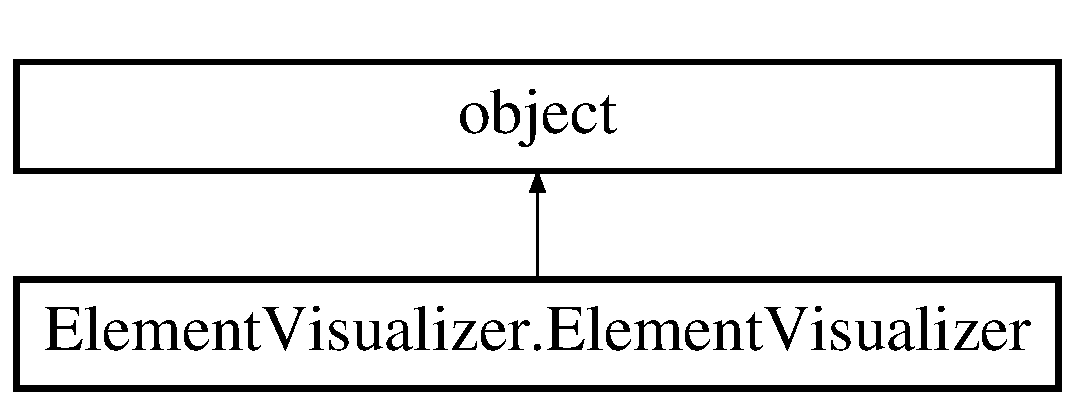
\includegraphics[height=2.000000cm]{class_element_visualizer_1_1_element_visualizer}
\end{center}
\end{figure}
\subsection*{Public Member Functions}
\begin{DoxyCompactItemize}
\item 
def \hyperlink{class_element_visualizer_1_1_element_visualizer_af8cdc78a3e01aeb46c3f0a6f18313267}{\+\_\+\+\_\+init\+\_\+\+\_\+} (self)
\begin{DoxyCompactList}\small\item\em Construct an \hyperlink{class_element_visualizer_1_1_element_visualizer}{Element\+Visualizer} with the default visualization settings. \end{DoxyCompactList}\item 
def \hyperlink{class_element_visualizer_1_1_element_visualizer_a62cc4d3f47385ae6d60b34b651456f29}{set\+Size} (self, size)
\begin{DoxyCompactList}\small\item\em Set the size of the \hyperlink{namespace_element}{Element} in the Bridge Visualization in pixels. \end{DoxyCompactList}\item 
def \hyperlink{class_element_visualizer_1_1_element_visualizer_a6021f693ae84d46c5e5d8fc27873ca7e}{get\+Size} (self)
\begin{DoxyCompactList}\small\item\em Get the size of the \hyperlink{namespace_element}{Element} in the Bridges Visualiation. \end{DoxyCompactList}\item 
def \hyperlink{class_element_visualizer_1_1_element_visualizer_a90429883a7814ab9571c1b5a0baa9e4e}{set\+Color} (self, a\+Color)
\begin{DoxyCompactList}\small\item\em Set the color of the \hyperlink{namespace_element}{Element} in the Bridges Visualization to \char`\"{}a\+Color\char`\"{}. \end{DoxyCompactList}\item 
def \hyperlink{class_element_visualizer_1_1_element_visualizer_a82a12847bbd1662462ef6493d240ee9d}{get\+Color} (self)
\begin{DoxyCompactList}\small\item\em Get the color of the \hyperlink{namespace_element}{Element} in the Bridges Visualization. \end{DoxyCompactList}\item 
def \hyperlink{class_element_visualizer_1_1_element_visualizer_a5a995818bc21ffba6bcab3c34220cf80}{get\+Shape} (self)
\begin{DoxyCompactList}\small\item\em Get the shape of the \hyperlink{namespace_element}{Element} in the Bridges Visualization. \end{DoxyCompactList}\item 
def \hyperlink{class_element_visualizer_1_1_element_visualizer_aee33522cc2e7dccf6471ba0fb6b8066d}{set\+Shape} (self, a\+Shape)
\begin{DoxyCompactList}\small\item\em Sets the shape of the \hyperlink{namespace_element}{Element} in the Bridges Visualization. \end{DoxyCompactList}\item 
def \hyperlink{class_element_visualizer_1_1_element_visualizer_aea9cae4dc99c63ee017ad1b7becd36fb}{set\+Opacity} (self, opacity)
\begin{DoxyCompactList}\small\item\em Sets the opacity of the \hyperlink{namespace_element}{Element} in the Bridges Visualization. \end{DoxyCompactList}\item 
def \hyperlink{class_element_visualizer_1_1_element_visualizer_a5ca091e52fb9ef498b08a63b783aa51d}{get\+Opacity} (self)
\begin{DoxyCompactList}\small\item\em Get the opacity of the \hyperlink{namespace_element}{Element} in the Bridges Visualization. \end{DoxyCompactList}\item 
def \hyperlink{class_element_visualizer_1_1_element_visualizer_ad128c758217718b95114a033e33824cf}{random\+Color} (self)
\begin{DoxyCompactList}\small\item\em The random\+Color method selects a random color from the available list of colors found in Validation.\+java and sets the color of the current element. \end{DoxyCompactList}\end{DoxyCompactItemize}
\subsection*{Static Public Attributes}
\begin{DoxyCompactItemize}
\item 
\hyperlink{class_element_visualizer_1_1_element_visualizer_a2c7c4e30a547a0269a4b918794068985}{properties} = Hash\+Map()
\end{DoxyCompactItemize}


\subsection{Detailed Description}
This class is used to store the visualization elements on the for the Bridges Visualiztion, including the color, shape, opacity, and size of the node. 

Objects of this class are stored as properties of all \hyperlink{namespace_element}{Element} subclasses. Generally, you will manipulating the \hyperlink{class_element_visualizer_1_1_element_visualizer}{Element\+Visualizer} returned from the \hyperlink{namespace_element}{Element} get\+Visualizer() method, and then call the set\+Visualizer() method on the \hyperlink{namespace_element}{Element} after changes have been made.\begin{DoxyVerb}generated source for class ElementVisualizer \end{DoxyVerb}
 

\subsection{Constructor \& Destructor Documentation}
\hypertarget{class_element_visualizer_1_1_element_visualizer_af8cdc78a3e01aeb46c3f0a6f18313267}{}\label{class_element_visualizer_1_1_element_visualizer_af8cdc78a3e01aeb46c3f0a6f18313267} 
\index{Element\+Visualizer\+::\+Element\+Visualizer@{Element\+Visualizer\+::\+Element\+Visualizer}!\+\_\+\+\_\+init\+\_\+\+\_\+@{\+\_\+\+\_\+init\+\_\+\+\_\+}}
\index{\+\_\+\+\_\+init\+\_\+\+\_\+@{\+\_\+\+\_\+init\+\_\+\+\_\+}!Element\+Visualizer\+::\+Element\+Visualizer@{Element\+Visualizer\+::\+Element\+Visualizer}}
\subsubsection{\texorpdfstring{\+\_\+\+\_\+init\+\_\+\+\_\+()}{\_\_init\_\_()}}
{\footnotesize\ttfamily def Element\+Visualizer.\+Element\+Visualizer.\+\_\+\+\_\+init\+\_\+\+\_\+ (\begin{DoxyParamCaption}\item[{}]{self }\end{DoxyParamCaption})}



Construct an \hyperlink{class_element_visualizer_1_1_element_visualizer}{Element\+Visualizer} with the default visualization settings. 

The default settings are color = green, opacity = 1.\+0, size = 10.\+0, shape = circle.\begin{DoxyVerb}generated source for method __init__ \end{DoxyVerb}
 

\subsection{Member Function Documentation}
\hypertarget{class_element_visualizer_1_1_element_visualizer_a82a12847bbd1662462ef6493d240ee9d}{}\label{class_element_visualizer_1_1_element_visualizer_a82a12847bbd1662462ef6493d240ee9d} 
\index{Element\+Visualizer\+::\+Element\+Visualizer@{Element\+Visualizer\+::\+Element\+Visualizer}!get\+Color@{get\+Color}}
\index{get\+Color@{get\+Color}!Element\+Visualizer\+::\+Element\+Visualizer@{Element\+Visualizer\+::\+Element\+Visualizer}}
\subsubsection{\texorpdfstring{get\+Color()}{getColor()}}
{\footnotesize\ttfamily def Element\+Visualizer.\+Element\+Visualizer.\+get\+Color (\begin{DoxyParamCaption}\item[{}]{self }\end{DoxyParamCaption})}



Get the color of the \hyperlink{namespace_element}{Element} in the Bridges Visualization. 

\begin{DoxyReturn}{Returns}
the string reprsenting the color of the \hyperlink{namespace_element}{Element} in the Bridges Visualization\begin{DoxyVerb}generated source for method getColor \end{DoxyVerb}
 
\end{DoxyReturn}
\hypertarget{class_element_visualizer_1_1_element_visualizer_a5ca091e52fb9ef498b08a63b783aa51d}{}\label{class_element_visualizer_1_1_element_visualizer_a5ca091e52fb9ef498b08a63b783aa51d} 
\index{Element\+Visualizer\+::\+Element\+Visualizer@{Element\+Visualizer\+::\+Element\+Visualizer}!get\+Opacity@{get\+Opacity}}
\index{get\+Opacity@{get\+Opacity}!Element\+Visualizer\+::\+Element\+Visualizer@{Element\+Visualizer\+::\+Element\+Visualizer}}
\subsubsection{\texorpdfstring{get\+Opacity()}{getOpacity()}}
{\footnotesize\ttfamily def Element\+Visualizer.\+Element\+Visualizer.\+get\+Opacity (\begin{DoxyParamCaption}\item[{}]{self }\end{DoxyParamCaption})}



Get the opacity of the \hyperlink{namespace_element}{Element} in the Bridges Visualization. 

\begin{DoxyReturn}{Returns}
the opacity value\begin{DoxyVerb}generated source for method getOpacity \end{DoxyVerb}
 
\end{DoxyReturn}
\hypertarget{class_element_visualizer_1_1_element_visualizer_a5a995818bc21ffba6bcab3c34220cf80}{}\label{class_element_visualizer_1_1_element_visualizer_a5a995818bc21ffba6bcab3c34220cf80} 
\index{Element\+Visualizer\+::\+Element\+Visualizer@{Element\+Visualizer\+::\+Element\+Visualizer}!get\+Shape@{get\+Shape}}
\index{get\+Shape@{get\+Shape}!Element\+Visualizer\+::\+Element\+Visualizer@{Element\+Visualizer\+::\+Element\+Visualizer}}
\subsubsection{\texorpdfstring{get\+Shape()}{getShape()}}
{\footnotesize\ttfamily def Element\+Visualizer.\+Element\+Visualizer.\+get\+Shape (\begin{DoxyParamCaption}\item[{}]{self }\end{DoxyParamCaption})}



Get the shape of the \hyperlink{namespace_element}{Element} in the Bridges Visualization. 

\begin{DoxyReturn}{Returns}
the string that represents the \hyperlink{namespace_element}{Element}\textquotesingle{}s shape in the Bridges Visualization.\begin{DoxyVerb}generated source for method getShape \end{DoxyVerb}
 
\end{DoxyReturn}
\hypertarget{class_element_visualizer_1_1_element_visualizer_a6021f693ae84d46c5e5d8fc27873ca7e}{}\label{class_element_visualizer_1_1_element_visualizer_a6021f693ae84d46c5e5d8fc27873ca7e} 
\index{Element\+Visualizer\+::\+Element\+Visualizer@{Element\+Visualizer\+::\+Element\+Visualizer}!get\+Size@{get\+Size}}
\index{get\+Size@{get\+Size}!Element\+Visualizer\+::\+Element\+Visualizer@{Element\+Visualizer\+::\+Element\+Visualizer}}
\subsubsection{\texorpdfstring{get\+Size()}{getSize()}}
{\footnotesize\ttfamily def Element\+Visualizer.\+Element\+Visualizer.\+get\+Size (\begin{DoxyParamCaption}\item[{}]{self }\end{DoxyParamCaption})}



Get the size of the \hyperlink{namespace_element}{Element} in the Bridges Visualiation. 

\begin{DoxyReturn}{Returns}
the size in pixels of the \hyperlink{namespace_element}{Element} in the Bridges Visualization\begin{DoxyVerb}generated source for method getSize \end{DoxyVerb}
 
\end{DoxyReturn}
\hypertarget{class_element_visualizer_1_1_element_visualizer_ad128c758217718b95114a033e33824cf}{}\label{class_element_visualizer_1_1_element_visualizer_ad128c758217718b95114a033e33824cf} 
\index{Element\+Visualizer\+::\+Element\+Visualizer@{Element\+Visualizer\+::\+Element\+Visualizer}!random\+Color@{random\+Color}}
\index{random\+Color@{random\+Color}!Element\+Visualizer\+::\+Element\+Visualizer@{Element\+Visualizer\+::\+Element\+Visualizer}}
\subsubsection{\texorpdfstring{random\+Color()}{randomColor()}}
{\footnotesize\ttfamily def Element\+Visualizer.\+Element\+Visualizer.\+random\+Color (\begin{DoxyParamCaption}\item[{}]{self }\end{DoxyParamCaption})}



The random\+Color method selects a random color from the available list of colors found in Validation.\+java and sets the color of the current element. 

\begin{DoxyReturn}{Returns}
a color name as a string value\begin{DoxyVerb}generated source for method randomColor \end{DoxyVerb}
 
\end{DoxyReturn}
\hypertarget{class_element_visualizer_1_1_element_visualizer_a90429883a7814ab9571c1b5a0baa9e4e}{}\label{class_element_visualizer_1_1_element_visualizer_a90429883a7814ab9571c1b5a0baa9e4e} 
\index{Element\+Visualizer\+::\+Element\+Visualizer@{Element\+Visualizer\+::\+Element\+Visualizer}!set\+Color@{set\+Color}}
\index{set\+Color@{set\+Color}!Element\+Visualizer\+::\+Element\+Visualizer@{Element\+Visualizer\+::\+Element\+Visualizer}}
\subsubsection{\texorpdfstring{set\+Color()}{setColor()}}
{\footnotesize\ttfamily def Element\+Visualizer.\+Element\+Visualizer.\+set\+Color (\begin{DoxyParamCaption}\item[{}]{self,  }\item[{}]{a\+Color }\end{DoxyParamCaption})}



Set the color of the \hyperlink{namespace_element}{Element} in the Bridges Visualization to \char`\"{}a\+Color\char`\"{}. 


\begin{DoxyParams}{Parameters}
{\em a\+Color} & the string reprsenting the color of the \hyperlink{namespace_element}{Element} in the Bridges Visualization\begin{DoxyVerb}generated source for method setColor \end{DoxyVerb}
 \\
\hline
\end{DoxyParams}
\hypertarget{class_element_visualizer_1_1_element_visualizer_aea9cae4dc99c63ee017ad1b7becd36fb}{}\label{class_element_visualizer_1_1_element_visualizer_aea9cae4dc99c63ee017ad1b7becd36fb} 
\index{Element\+Visualizer\+::\+Element\+Visualizer@{Element\+Visualizer\+::\+Element\+Visualizer}!set\+Opacity@{set\+Opacity}}
\index{set\+Opacity@{set\+Opacity}!Element\+Visualizer\+::\+Element\+Visualizer@{Element\+Visualizer\+::\+Element\+Visualizer}}
\subsubsection{\texorpdfstring{set\+Opacity()}{setOpacity()}}
{\footnotesize\ttfamily def Element\+Visualizer.\+Element\+Visualizer.\+set\+Opacity (\begin{DoxyParamCaption}\item[{}]{self,  }\item[{}]{opacity }\end{DoxyParamCaption})}



Sets the opacity of the \hyperlink{namespace_element}{Element} in the Bridges Visualization. 


\begin{DoxyParams}{Parameters}
{\em opacity} & a double between 0 and 1 representing how transparent the node should be on the Bridges Visualization. 0 for invisible, 1 for fully visible, a decimal between 0 and 1 for varying transparency.\begin{DoxyVerb}generated source for method setOpacity \end{DoxyVerb}
 \\
\hline
\end{DoxyParams}
\hypertarget{class_element_visualizer_1_1_element_visualizer_aee33522cc2e7dccf6471ba0fb6b8066d}{}\label{class_element_visualizer_1_1_element_visualizer_aee33522cc2e7dccf6471ba0fb6b8066d} 
\index{Element\+Visualizer\+::\+Element\+Visualizer@{Element\+Visualizer\+::\+Element\+Visualizer}!set\+Shape@{set\+Shape}}
\index{set\+Shape@{set\+Shape}!Element\+Visualizer\+::\+Element\+Visualizer@{Element\+Visualizer\+::\+Element\+Visualizer}}
\subsubsection{\texorpdfstring{set\+Shape()}{setShape()}}
{\footnotesize\ttfamily def Element\+Visualizer.\+Element\+Visualizer.\+set\+Shape (\begin{DoxyParamCaption}\item[{}]{self,  }\item[{}]{a\+Shape }\end{DoxyParamCaption})}



Sets the shape of the \hyperlink{namespace_element}{Element} in the Bridges Visualization. 


\begin{DoxyParams}{Parameters}
{\em a\+Shape} & the string representing the shape of the \hyperlink{namespace_element}{Element} in the Bridges Visualization\begin{DoxyVerb}generated source for method setShape \end{DoxyVerb}
 \\
\hline
\end{DoxyParams}
\hypertarget{class_element_visualizer_1_1_element_visualizer_a62cc4d3f47385ae6d60b34b651456f29}{}\label{class_element_visualizer_1_1_element_visualizer_a62cc4d3f47385ae6d60b34b651456f29} 
\index{Element\+Visualizer\+::\+Element\+Visualizer@{Element\+Visualizer\+::\+Element\+Visualizer}!set\+Size@{set\+Size}}
\index{set\+Size@{set\+Size}!Element\+Visualizer\+::\+Element\+Visualizer@{Element\+Visualizer\+::\+Element\+Visualizer}}
\subsubsection{\texorpdfstring{set\+Size()}{setSize()}}
{\footnotesize\ttfamily def Element\+Visualizer.\+Element\+Visualizer.\+set\+Size (\begin{DoxyParamCaption}\item[{}]{self,  }\item[{}]{size }\end{DoxyParamCaption})}



Set the size of the \hyperlink{namespace_element}{Element} in the Bridge Visualization in pixels. 


\begin{DoxyParams}{Parameters}
{\em size} & the pixel size of the \hyperlink{namespace_element}{Element} in the Bridges Visualization\begin{DoxyVerb}generated source for method setSize \end{DoxyVerb}
 \\
\hline
\end{DoxyParams}


\subsection{Member Data Documentation}
\hypertarget{class_element_visualizer_1_1_element_visualizer_a2c7c4e30a547a0269a4b918794068985}{}\label{class_element_visualizer_1_1_element_visualizer_a2c7c4e30a547a0269a4b918794068985} 
\index{Element\+Visualizer\+::\+Element\+Visualizer@{Element\+Visualizer\+::\+Element\+Visualizer}!properties@{properties}}
\index{properties@{properties}!Element\+Visualizer\+::\+Element\+Visualizer@{Element\+Visualizer\+::\+Element\+Visualizer}}
\subsubsection{\texorpdfstring{properties}{properties}}
{\footnotesize\ttfamily Element\+Visualizer.\+Element\+Visualizer.\+properties = Hash\+Map()\hspace{0.3cm}{\ttfamily [static]}}



The documentation for this class was generated from the following file\+:\begin{DoxyCompactItemize}
\item 
/\+Users/kalpathi/gr/bridges/client/python/src/\hyperlink{_element_visualizer_8py}{Element\+Visualizer.\+py}\end{DoxyCompactItemize}

\hypertarget{class_game_1_1_game}{}\section{Game.\+Game Class Reference}
\label{class_game_1_1_game}\index{Game.\+Game@{Game.\+Game}}
\subsection*{Public Member Functions}
\begin{DoxyCompactItemize}
\item 
def \hyperlink{class_game_1_1_game_a527f0ebbb5bce3e8cdfc3d4ff8a983a5}{\+\_\+\+\_\+init\+\_\+\+\_\+}
\item 
def \hyperlink{class_game_1_1_game_a8df95bdf87496f6ffdee1362b5c368f1}{get\+Title} (self)
\item 
def \hyperlink{class_game_1_1_game_a5c76d56082ee99757bfb8afbd596c611}{set\+Title} (self, \hyperlink{class_game_1_1_game_aa5495f06f46f1871c8736bca793ebcbc}{title})
\item 
def \hyperlink{class_game_1_1_game_aadaee85d41d7b52b519640d96404eb8f}{get\+Platform} (self)
\item 
def \hyperlink{class_game_1_1_game_a4b42643dee147238e1f1edf49b20cb9f}{set\+Platform} (self, \hyperlink{class_game_1_1_game_aa90b68ce03516874d8636bbf49fdc39e}{platform})
\item 
def \hyperlink{class_game_1_1_game_aa7856b02cfbffe83d5c7e05af9ce95dc}{get\+Rating} (self)
\item 
def \hyperlink{class_game_1_1_game_ae0b53653d5a9d4f0f3d3fd266f1d2d49}{set\+Rating} (self, \hyperlink{class_game_1_1_game_a274df8eb8d5dd182acd07582fe0f1e7e}{rating})
\item 
def \hyperlink{class_game_1_1_game_ae6d65e66c29cc6f633d9caba9dcc2a2c}{get\+Genre} (self)
\item 
def \hyperlink{class_game_1_1_game_a0d430c9fba04a7e02814f2628421013d}{set\+Genre} (self, \hyperlink{class_game_1_1_game_a4ab88fbd19810760dbf5be97432fe20f}{genre})
\end{DoxyCompactItemize}
\subsection*{Public Attributes}
\begin{DoxyCompactItemize}
\item 
\hyperlink{class_game_1_1_game_aa5495f06f46f1871c8736bca793ebcbc}{title}
\item 
\hyperlink{class_game_1_1_game_aa90b68ce03516874d8636bbf49fdc39e}{platform}
\item 
\hyperlink{class_game_1_1_game_a274df8eb8d5dd182acd07582fe0f1e7e}{rating}
\item 
\hyperlink{class_game_1_1_game_a4ab88fbd19810760dbf5be97432fe20f}{genre}
\end{DoxyCompactItemize}


\subsection{Constructor \& Destructor Documentation}
\hypertarget{class_game_1_1_game_a527f0ebbb5bce3e8cdfc3d4ff8a983a5}{}\index{Game\+::\+Game@{Game\+::\+Game}!\+\_\+\+\_\+init\+\_\+\+\_\+@{\+\_\+\+\_\+init\+\_\+\+\_\+}}
\index{\+\_\+\+\_\+init\+\_\+\+\_\+@{\+\_\+\+\_\+init\+\_\+\+\_\+}!Game\+::\+Game@{Game\+::\+Game}}
\subsubsection[{\+\_\+\+\_\+init\+\_\+\+\_\+}]{\setlength{\rightskip}{0pt plus 5cm}def Game.\+Game.\+\_\+\+\_\+init\+\_\+\+\_\+ (
\begin{DoxyParamCaption}
\item[{}]{self, }
\item[{}]{title = {\ttfamily None}, }
\item[{}]{platform = {\ttfamily None}, }
\item[{}]{rating = {\ttfamily None}, }
\item[{}]{genre = {\ttfamily None}}
\end{DoxyParamCaption}
)}\label{class_game_1_1_game_a527f0ebbb5bce3e8cdfc3d4ff8a983a5}


\subsection{Member Function Documentation}
\hypertarget{class_game_1_1_game_ae6d65e66c29cc6f633d9caba9dcc2a2c}{}\index{Game\+::\+Game@{Game\+::\+Game}!get\+Genre@{get\+Genre}}
\index{get\+Genre@{get\+Genre}!Game\+::\+Game@{Game\+::\+Game}}
\subsubsection[{get\+Genre(self)}]{\setlength{\rightskip}{0pt plus 5cm}def Game.\+Game.\+get\+Genre (
\begin{DoxyParamCaption}
\item[{}]{self}
\end{DoxyParamCaption}
)}\label{class_game_1_1_game_ae6d65e66c29cc6f633d9caba9dcc2a2c}
\hypertarget{class_game_1_1_game_aadaee85d41d7b52b519640d96404eb8f}{}\index{Game\+::\+Game@{Game\+::\+Game}!get\+Platform@{get\+Platform}}
\index{get\+Platform@{get\+Platform}!Game\+::\+Game@{Game\+::\+Game}}
\subsubsection[{get\+Platform(self)}]{\setlength{\rightskip}{0pt plus 5cm}def Game.\+Game.\+get\+Platform (
\begin{DoxyParamCaption}
\item[{}]{self}
\end{DoxyParamCaption}
)}\label{class_game_1_1_game_aadaee85d41d7b52b519640d96404eb8f}
\hypertarget{class_game_1_1_game_aa7856b02cfbffe83d5c7e05af9ce95dc}{}\index{Game\+::\+Game@{Game\+::\+Game}!get\+Rating@{get\+Rating}}
\index{get\+Rating@{get\+Rating}!Game\+::\+Game@{Game\+::\+Game}}
\subsubsection[{get\+Rating(self)}]{\setlength{\rightskip}{0pt plus 5cm}def Game.\+Game.\+get\+Rating (
\begin{DoxyParamCaption}
\item[{}]{self}
\end{DoxyParamCaption}
)}\label{class_game_1_1_game_aa7856b02cfbffe83d5c7e05af9ce95dc}
\hypertarget{class_game_1_1_game_a8df95bdf87496f6ffdee1362b5c368f1}{}\index{Game\+::\+Game@{Game\+::\+Game}!get\+Title@{get\+Title}}
\index{get\+Title@{get\+Title}!Game\+::\+Game@{Game\+::\+Game}}
\subsubsection[{get\+Title(self)}]{\setlength{\rightskip}{0pt plus 5cm}def Game.\+Game.\+get\+Title (
\begin{DoxyParamCaption}
\item[{}]{self}
\end{DoxyParamCaption}
)}\label{class_game_1_1_game_a8df95bdf87496f6ffdee1362b5c368f1}
\hypertarget{class_game_1_1_game_a0d430c9fba04a7e02814f2628421013d}{}\index{Game\+::\+Game@{Game\+::\+Game}!set\+Genre@{set\+Genre}}
\index{set\+Genre@{set\+Genre}!Game\+::\+Game@{Game\+::\+Game}}
\subsubsection[{set\+Genre(self, genre)}]{\setlength{\rightskip}{0pt plus 5cm}def Game.\+Game.\+set\+Genre (
\begin{DoxyParamCaption}
\item[{}]{self, }
\item[{}]{genre}
\end{DoxyParamCaption}
)}\label{class_game_1_1_game_a0d430c9fba04a7e02814f2628421013d}
\hypertarget{class_game_1_1_game_a4b42643dee147238e1f1edf49b20cb9f}{}\index{Game\+::\+Game@{Game\+::\+Game}!set\+Platform@{set\+Platform}}
\index{set\+Platform@{set\+Platform}!Game\+::\+Game@{Game\+::\+Game}}
\subsubsection[{set\+Platform(self, platform)}]{\setlength{\rightskip}{0pt plus 5cm}def Game.\+Game.\+set\+Platform (
\begin{DoxyParamCaption}
\item[{}]{self, }
\item[{}]{platform}
\end{DoxyParamCaption}
)}\label{class_game_1_1_game_a4b42643dee147238e1f1edf49b20cb9f}
\hypertarget{class_game_1_1_game_ae0b53653d5a9d4f0f3d3fd266f1d2d49}{}\index{Game\+::\+Game@{Game\+::\+Game}!set\+Rating@{set\+Rating}}
\index{set\+Rating@{set\+Rating}!Game\+::\+Game@{Game\+::\+Game}}
\subsubsection[{set\+Rating(self, rating)}]{\setlength{\rightskip}{0pt plus 5cm}def Game.\+Game.\+set\+Rating (
\begin{DoxyParamCaption}
\item[{}]{self, }
\item[{}]{rating}
\end{DoxyParamCaption}
)}\label{class_game_1_1_game_ae0b53653d5a9d4f0f3d3fd266f1d2d49}
\hypertarget{class_game_1_1_game_a5c76d56082ee99757bfb8afbd596c611}{}\index{Game\+::\+Game@{Game\+::\+Game}!set\+Title@{set\+Title}}
\index{set\+Title@{set\+Title}!Game\+::\+Game@{Game\+::\+Game}}
\subsubsection[{set\+Title(self, title)}]{\setlength{\rightskip}{0pt plus 5cm}def Game.\+Game.\+set\+Title (
\begin{DoxyParamCaption}
\item[{}]{self, }
\item[{}]{title}
\end{DoxyParamCaption}
)}\label{class_game_1_1_game_a5c76d56082ee99757bfb8afbd596c611}


\subsection{Member Data Documentation}
\hypertarget{class_game_1_1_game_a4ab88fbd19810760dbf5be97432fe20f}{}\index{Game\+::\+Game@{Game\+::\+Game}!genre@{genre}}
\index{genre@{genre}!Game\+::\+Game@{Game\+::\+Game}}
\subsubsection[{genre}]{\setlength{\rightskip}{0pt plus 5cm}Game.\+Game.\+genre}\label{class_game_1_1_game_a4ab88fbd19810760dbf5be97432fe20f}
\hypertarget{class_game_1_1_game_aa90b68ce03516874d8636bbf49fdc39e}{}\index{Game\+::\+Game@{Game\+::\+Game}!platform@{platform}}
\index{platform@{platform}!Game\+::\+Game@{Game\+::\+Game}}
\subsubsection[{platform}]{\setlength{\rightskip}{0pt plus 5cm}Game.\+Game.\+platform}\label{class_game_1_1_game_aa90b68ce03516874d8636bbf49fdc39e}
\hypertarget{class_game_1_1_game_a274df8eb8d5dd182acd07582fe0f1e7e}{}\index{Game\+::\+Game@{Game\+::\+Game}!rating@{rating}}
\index{rating@{rating}!Game\+::\+Game@{Game\+::\+Game}}
\subsubsection[{rating}]{\setlength{\rightskip}{0pt plus 5cm}Game.\+Game.\+rating}\label{class_game_1_1_game_a274df8eb8d5dd182acd07582fe0f1e7e}
\hypertarget{class_game_1_1_game_aa5495f06f46f1871c8736bca793ebcbc}{}\index{Game\+::\+Game@{Game\+::\+Game}!title@{title}}
\index{title@{title}!Game\+::\+Game@{Game\+::\+Game}}
\subsubsection[{title}]{\setlength{\rightskip}{0pt plus 5cm}Game.\+Game.\+title}\label{class_game_1_1_game_aa5495f06f46f1871c8736bca793ebcbc}


The documentation for this class was generated from the following file\+:\begin{DoxyCompactItemize}
\item 
/\+Users/krs/gr/bridges/bridges17/python/src/data\+\_\+src\+\_\+dependent/\hyperlink{_game_8py}{Game.\+py}\end{DoxyCompactItemize}

\hypertarget{class_graph_adj_list_1_1_graph_adj_list}{}\section{Graph\+Adj\+List.\+Graph\+Adj\+List Class Reference}
\label{class_graph_adj_list_1_1_graph_adj_list}\index{Graph\+Adj\+List.\+Graph\+Adj\+List@{Graph\+Adj\+List.\+Graph\+Adj\+List}}


The \hyperlink{class_graph_adj_list_1_1_graph_adj_list}{Graph\+Adj\+List} class can be used to represent adjacency list based graphs in B\+R\+I\+D\+G\+ES.  


Inheritance diagram for Graph\+Adj\+List.\+Graph\+Adj\+List\+:\begin{figure}[H]
\begin{center}
\leavevmode
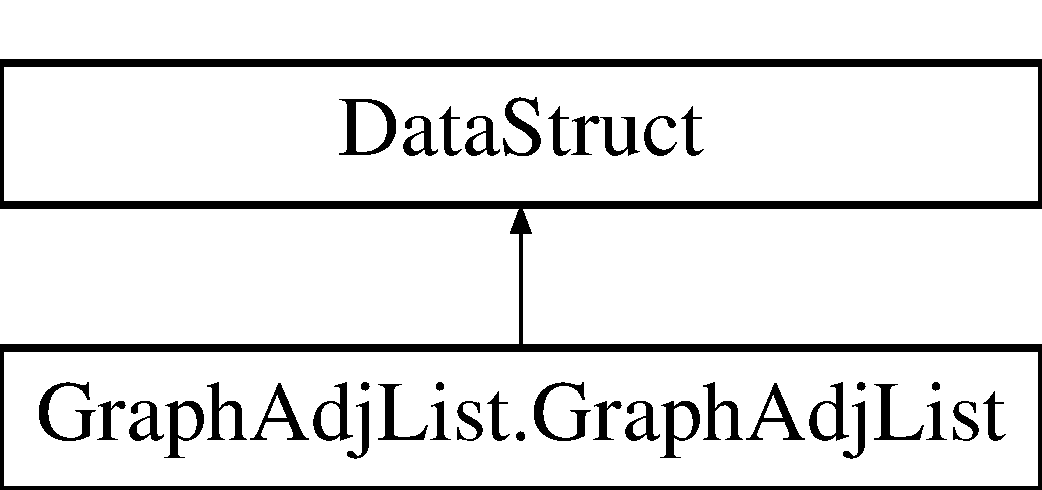
\includegraphics[height=2.000000cm]{class_graph_adj_list_1_1_graph_adj_list}
\end{center}
\end{figure}
\subsection*{Public Member Functions}
\begin{DoxyCompactItemize}
\item 
def \hyperlink{class_graph_adj_list_1_1_graph_adj_list_a045be8de7a7695b8eac07feb9011b73d}{\+\_\+\+\_\+init\+\_\+\+\_\+} (self)
\begin{DoxyCompactList}\small\item\em Constructor. \end{DoxyCompactList}\item 
def \hyperlink{class_graph_adj_list_1_1_graph_adj_list_a19fd235cb56eaaf5335331088bb52c37}{get\+Data\+Struct\+Type} (self)
\begin{DoxyCompactList}\small\item\em This method gets the data structure type. \end{DoxyCompactList}\item 
def \hyperlink{class_graph_adj_list_1_1_graph_adj_list_ab2f7025978821c01436cc773957bb9c5}{add\+Vertex} (self, k, e)
\begin{DoxyCompactList}\small\item\em Adds a new vertex to the graph, initializes the adjacency list; user is responsible for checking if the vertex already exists. \end{DoxyCompactList}\item 
def \hyperlink{class_graph_adj_list_1_1_graph_adj_list_a52d80ff8e432cabad99cc77feb82a295}{add\+Edge} (self, src, dest)
\begin{DoxyCompactList}\small\item\em Adds a new edge to the graph, adds it to that vertex\textquotesingle{}s adjacency list; user is responsible for checking if the vertex already exists. \end{DoxyCompactList}\item 
def \hyperlink{class_graph_adj_list_1_1_graph_adj_list_a33234517232ecd8a4fab8ded3dcdd85d}{add\+Edge\+\_\+0} (self, src, dest, weight)
\begin{DoxyCompactList}\small\item\em Adds a new edge to the graph, adds it to that vertex\textquotesingle{}s adjacency list; user is responsible for checking if the vertex already exists. \end{DoxyCompactList}\item 
def \hyperlink{class_graph_adj_list_1_1_graph_adj_list_a5921cc09aba4d4b61d5cb5e97ee6473f}{get\+Vertices} (self)
\begin{DoxyCompactList}\small\item\em This method returns the graph nodes. \end{DoxyCompactList}\item 
def \hyperlink{class_graph_adj_list_1_1_graph_adj_list_a8f0e2f62373963562f2c28bfb1513bc1}{get\+Vertex} (self, key)
\begin{DoxyCompactList}\small\item\em This is a convenience method to retrieve a vertex given its key. \end{DoxyCompactList}\item 
def \hyperlink{class_graph_adj_list_1_1_graph_adj_list_ae5fe3c73d73d417121b0d3f39d9a6ccf}{get\+Adjacency\+List} (self)
\begin{DoxyCompactList}\small\item\em Gets the adjacency list (of type S\+Lelement$<$\+Edge$>$ ) \end{DoxyCompactList}\item 
def \hyperlink{class_graph_adj_list_1_1_graph_adj_list_ae446e3a3cd1c8e04faf600ac46dbfddc}{get\+Adjacency\+List\+\_\+0} (self, vertex)
\begin{DoxyCompactList}\small\item\em Gets the adjacency list (of type \hyperlink{namespace_s_lelement}{S\+Lelement}$<$\hyperlink{namespace_edge}{Edge} $<$\+K$>$ $>$ of a vertex) \end{DoxyCompactList}\item 
def \hyperlink{class_graph_adj_list_1_1_graph_adj_list_ac8e04d8c44a0a7f117e38215c593845e}{get\+Link\+Visualizer} (self, src, dest)
\begin{DoxyCompactList}\small\item\em This is a convenience method to simplify access to the link visualizer; the method assumes the vertex names point to existing vertices, else an exception is thrown. \end{DoxyCompactList}\item 
def \hyperlink{class_graph_adj_list_1_1_graph_adj_list_ac5526b72818cd4f4f939a42cb173ada3}{get\+Visualizer} (self, vertex)
\begin{DoxyCompactList}\small\item\em This is a convenience method to simplify access to the element visualizer; the method assumes the vertex name points to an existing vertice, else an exception is thrown. \end{DoxyCompactList}\item 
def \hyperlink{class_graph_adj_list_1_1_graph_adj_list_abb989d64385323cd0032c74c85b449fa}{get\+Data\+Structure\+Representation} (self)
\begin{DoxyCompactList}\small\item\em Get the J\+S\+ON representation of the the data structure. \end{DoxyCompactList}\end{DoxyCompactItemize}
\subsection*{Static Public Attributes}
\begin{DoxyCompactItemize}
\item 
\hyperlink{class_graph_adj_list_1_1_graph_adj_list_a47f4552a36c0fdc7d7599a7b5b47177d}{vertices} = Hash\+Map()
\item 
\hyperlink{class_graph_adj_list_1_1_graph_adj_list_adf27f860d178d9d0f0aa3c3a6c45afe9}{adj\+\_\+list} = Hash\+Map()
\end{DoxyCompactItemize}


\subsection{Detailed Description}
The \hyperlink{class_graph_adj_list_1_1_graph_adj_list}{Graph\+Adj\+List} class can be used to represent adjacency list based graphs in B\+R\+I\+D\+G\+ES. 

The \hyperlink{class_graph_adj_list_1_1_graph_adj_list}{Graph\+Adj\+List} class can be used to represent adjacency list based graphs in B\+R\+I\+D\+G\+ES; it takes 2 generic parameters\+: (1) K, which is an orderable key value used in accessing vertices (in constant time) using a hashmap. This permits data sets that need to be accessed by keys that are strings, and (2) E, an application defined type, and used in the \hyperlink{namespace_edge}{Edge} representation. The class is simply a wrapper around the Java Hashmap class and, thus, derives all its operations from it. B\+R\+I\+D\+G\+ES provides methods to visualize the graph and its contents.

The vertices of the graph are held in a Java hashmap, for near constant time access; this lets us use strings or integral ids for vertices. The adjacency lists, also a Java hashmap are built for each vertex and contain the edge (terminating vertex id, weight) in the \hyperlink{namespace_edge}{Edge} structure, defined separately. Adjacency lists are singly linked lists using the B\+R\+I\+D\+G\+ES \hyperlink{namespace_s_lelement}{S\+Lelement}.

Convenience methods are provided to add vertices and edges to the graph as well as retrieve the adjacency list of a vertex, given its id.

\begin{DoxyAuthor}{Author}
Kalpathi Subramanian
\end{DoxyAuthor}
\begin{DoxyDate}{Date}
6/29/15, 5/18/17
\end{DoxyDate}

\begin{DoxyParams}{Parameters}
{\em $<$\+E$>$} & application/user defined type used as part of vertices and edges \\
\hline
{\em $<$\+K$>$} & orderable key (string, int, etc) that is used to index into vertex structure, for fast access\\
\hline
\end{DoxyParams}
\begin{DoxySeeAlso}{See also}
Example tutorial at 
\end{DoxySeeAlso}
\href{http://bridgesuncc.github.io/Hello_World_Tutorials/Graph.html@verbatim}{\tt http\+://bridgesuncc.\+github.\+io/\+Hello\+\_\+\+World\+\_\+\+Tutorials/\+Graph.\+html@verbatim} generated source for class \hyperlink{class_graph_adj_list_1_1_graph_adj_list}{Graph\+Adj\+List}  

\subsection{Constructor \& Destructor Documentation}
\hypertarget{class_graph_adj_list_1_1_graph_adj_list_a045be8de7a7695b8eac07feb9011b73d}{}\label{class_graph_adj_list_1_1_graph_adj_list_a045be8de7a7695b8eac07feb9011b73d} 
\index{Graph\+Adj\+List\+::\+Graph\+Adj\+List@{Graph\+Adj\+List\+::\+Graph\+Adj\+List}!\+\_\+\+\_\+init\+\_\+\+\_\+@{\+\_\+\+\_\+init\+\_\+\+\_\+}}
\index{\+\_\+\+\_\+init\+\_\+\+\_\+@{\+\_\+\+\_\+init\+\_\+\+\_\+}!Graph\+Adj\+List\+::\+Graph\+Adj\+List@{Graph\+Adj\+List\+::\+Graph\+Adj\+List}}
\subsubsection{\texorpdfstring{\+\_\+\+\_\+init\+\_\+\+\_\+()}{\_\_init\_\_()}}
{\footnotesize\ttfamily def Graph\+Adj\+List.\+Graph\+Adj\+List.\+\_\+\+\_\+init\+\_\+\+\_\+ (\begin{DoxyParamCaption}\item[{}]{self }\end{DoxyParamCaption})}



Constructor. 

\begin{DoxyVerb}generated source for method __init__ \end{DoxyVerb}
 

\subsection{Member Function Documentation}
\hypertarget{class_graph_adj_list_1_1_graph_adj_list_a52d80ff8e432cabad99cc77feb82a295}{}\label{class_graph_adj_list_1_1_graph_adj_list_a52d80ff8e432cabad99cc77feb82a295} 
\index{Graph\+Adj\+List\+::\+Graph\+Adj\+List@{Graph\+Adj\+List\+::\+Graph\+Adj\+List}!add\+Edge@{add\+Edge}}
\index{add\+Edge@{add\+Edge}!Graph\+Adj\+List\+::\+Graph\+Adj\+List@{Graph\+Adj\+List\+::\+Graph\+Adj\+List}}
\subsubsection{\texorpdfstring{add\+Edge()}{addEdge()}}
{\footnotesize\ttfamily def Graph\+Adj\+List.\+Graph\+Adj\+List.\+add\+Edge (\begin{DoxyParamCaption}\item[{}]{self,  }\item[{}]{src,  }\item[{}]{dest }\end{DoxyParamCaption})}



Adds a new edge to the graph, adds it to that vertex\textquotesingle{}s adjacency list; user is responsible for checking if the vertex already exists. 

This version assumes a default edge weight of 1.


\begin{DoxyParams}{Parameters}
{\em src} & -\/ source vertex of edge \\
\hline
{\em dest} & -\/ destination vertex of edge\begin{DoxyVerb}generated source for method addEdge \end{DoxyVerb}
 \\
\hline
\end{DoxyParams}
\hypertarget{class_graph_adj_list_1_1_graph_adj_list_a33234517232ecd8a4fab8ded3dcdd85d}{}\label{class_graph_adj_list_1_1_graph_adj_list_a33234517232ecd8a4fab8ded3dcdd85d} 
\index{Graph\+Adj\+List\+::\+Graph\+Adj\+List@{Graph\+Adj\+List\+::\+Graph\+Adj\+List}!add\+Edge\+\_\+0@{add\+Edge\+\_\+0}}
\index{add\+Edge\+\_\+0@{add\+Edge\+\_\+0}!Graph\+Adj\+List\+::\+Graph\+Adj\+List@{Graph\+Adj\+List\+::\+Graph\+Adj\+List}}
\subsubsection{\texorpdfstring{add\+Edge\+\_\+0()}{addEdge\_0()}}
{\footnotesize\ttfamily def Graph\+Adj\+List.\+Graph\+Adj\+List.\+add\+Edge\+\_\+0 (\begin{DoxyParamCaption}\item[{}]{self,  }\item[{}]{src,  }\item[{}]{dest,  }\item[{}]{weight }\end{DoxyParamCaption})}



Adds a new edge to the graph, adds it to that vertex\textquotesingle{}s adjacency list; user is responsible for checking if the vertex already exists. 


\begin{DoxyParams}{Parameters}
{\em src} & -\/ source vertex of edge \\
\hline
{\em dest} & -\/ destination vertex of edge \\
\hline
{\em weight} & -\/ edge weight\begin{DoxyVerb}generated source for method addEdge_0 \end{DoxyVerb}
 \\
\hline
\end{DoxyParams}
\hypertarget{class_graph_adj_list_1_1_graph_adj_list_ab2f7025978821c01436cc773957bb9c5}{}\label{class_graph_adj_list_1_1_graph_adj_list_ab2f7025978821c01436cc773957bb9c5} 
\index{Graph\+Adj\+List\+::\+Graph\+Adj\+List@{Graph\+Adj\+List\+::\+Graph\+Adj\+List}!add\+Vertex@{add\+Vertex}}
\index{add\+Vertex@{add\+Vertex}!Graph\+Adj\+List\+::\+Graph\+Adj\+List@{Graph\+Adj\+List\+::\+Graph\+Adj\+List}}
\subsubsection{\texorpdfstring{add\+Vertex()}{addVertex()}}
{\footnotesize\ttfamily def Graph\+Adj\+List.\+Graph\+Adj\+List.\+add\+Vertex (\begin{DoxyParamCaption}\item[{}]{self,  }\item[{}]{k,  }\item[{}]{e }\end{DoxyParamCaption})}



Adds a new vertex to the graph, initializes the adjacency list; user is responsible for checking if the vertex already exists. 

This method will replace the value for this key


\begin{DoxyParams}{Parameters}
{\em k} & -\/ vertex id \\
\hline
{\em E} & -\/ vertex info, currently used as a label by default\\
\hline
\end{DoxyParams}
\begin{DoxyReturn}{Returns}
none\begin{DoxyVerb}generated source for method addVertex \end{DoxyVerb}
 
\end{DoxyReturn}
\hypertarget{class_graph_adj_list_1_1_graph_adj_list_ae5fe3c73d73d417121b0d3f39d9a6ccf}{}\label{class_graph_adj_list_1_1_graph_adj_list_ae5fe3c73d73d417121b0d3f39d9a6ccf} 
\index{Graph\+Adj\+List\+::\+Graph\+Adj\+List@{Graph\+Adj\+List\+::\+Graph\+Adj\+List}!get\+Adjacency\+List@{get\+Adjacency\+List}}
\index{get\+Adjacency\+List@{get\+Adjacency\+List}!Graph\+Adj\+List\+::\+Graph\+Adj\+List@{Graph\+Adj\+List\+::\+Graph\+Adj\+List}}
\subsubsection{\texorpdfstring{get\+Adjacency\+List()}{getAdjacencyList()}}
{\footnotesize\ttfamily def Graph\+Adj\+List.\+Graph\+Adj\+List.\+get\+Adjacency\+List (\begin{DoxyParamCaption}\item[{}]{self }\end{DoxyParamCaption})}



Gets the adjacency list (of type S\+Lelement$<$\+Edge$>$ ) 

\begin{DoxyReturn}{Returns}
-\/ the graph\textquotesingle{}s adjacency lists\begin{DoxyVerb}generated source for method getAdjacencyList \end{DoxyVerb}
 
\end{DoxyReturn}
\hypertarget{class_graph_adj_list_1_1_graph_adj_list_ae446e3a3cd1c8e04faf600ac46dbfddc}{}\label{class_graph_adj_list_1_1_graph_adj_list_ae446e3a3cd1c8e04faf600ac46dbfddc} 
\index{Graph\+Adj\+List\+::\+Graph\+Adj\+List@{Graph\+Adj\+List\+::\+Graph\+Adj\+List}!get\+Adjacency\+List\+\_\+0@{get\+Adjacency\+List\+\_\+0}}
\index{get\+Adjacency\+List\+\_\+0@{get\+Adjacency\+List\+\_\+0}!Graph\+Adj\+List\+::\+Graph\+Adj\+List@{Graph\+Adj\+List\+::\+Graph\+Adj\+List}}
\subsubsection{\texorpdfstring{get\+Adjacency\+List\+\_\+0()}{getAdjacencyList\_0()}}
{\footnotesize\ttfamily def Graph\+Adj\+List.\+Graph\+Adj\+List.\+get\+Adjacency\+List\+\_\+0 (\begin{DoxyParamCaption}\item[{}]{self,  }\item[{}]{vertex }\end{DoxyParamCaption})}



Gets the adjacency list (of type \hyperlink{namespace_s_lelement}{S\+Lelement}$<$\hyperlink{namespace_edge}{Edge} $<$\+K$>$ $>$ of a vertex) 


\begin{DoxyParams}{Parameters}
{\em -\/} & vertex key\\
\hline
\end{DoxyParams}
\begin{DoxyReturn}{Returns}
-\/ the graph\textquotesingle{}s adjacency list corresponding to this vertex\begin{DoxyVerb}generated source for method getAdjacencyList_0 \end{DoxyVerb}
 
\end{DoxyReturn}
\hypertarget{class_graph_adj_list_1_1_graph_adj_list_a19fd235cb56eaaf5335331088bb52c37}{}\label{class_graph_adj_list_1_1_graph_adj_list_a19fd235cb56eaaf5335331088bb52c37} 
\index{Graph\+Adj\+List\+::\+Graph\+Adj\+List@{Graph\+Adj\+List\+::\+Graph\+Adj\+List}!get\+Data\+Struct\+Type@{get\+Data\+Struct\+Type}}
\index{get\+Data\+Struct\+Type@{get\+Data\+Struct\+Type}!Graph\+Adj\+List\+::\+Graph\+Adj\+List@{Graph\+Adj\+List\+::\+Graph\+Adj\+List}}
\subsubsection{\texorpdfstring{get\+Data\+Struct\+Type()}{getDataStructType()}}
{\footnotesize\ttfamily def Graph\+Adj\+List.\+Graph\+Adj\+List.\+get\+Data\+Struct\+Type (\begin{DoxyParamCaption}\item[{}]{self }\end{DoxyParamCaption})}



This method gets the data structure type. 

\begin{DoxyReturn}{Returns}
The date structure type as a string\begin{DoxyVerb}generated source for method getDataStructType \end{DoxyVerb}
 
\end{DoxyReturn}
\hypertarget{class_graph_adj_list_1_1_graph_adj_list_abb989d64385323cd0032c74c85b449fa}{}\label{class_graph_adj_list_1_1_graph_adj_list_abb989d64385323cd0032c74c85b449fa} 
\index{Graph\+Adj\+List\+::\+Graph\+Adj\+List@{Graph\+Adj\+List\+::\+Graph\+Adj\+List}!get\+Data\+Structure\+Representation@{get\+Data\+Structure\+Representation}}
\index{get\+Data\+Structure\+Representation@{get\+Data\+Structure\+Representation}!Graph\+Adj\+List\+::\+Graph\+Adj\+List@{Graph\+Adj\+List\+::\+Graph\+Adj\+List}}
\subsubsection{\texorpdfstring{get\+Data\+Structure\+Representation()}{getDataStructureRepresentation()}}
{\footnotesize\ttfamily def Graph\+Adj\+List.\+Graph\+Adj\+List.\+get\+Data\+Structure\+Representation (\begin{DoxyParamCaption}\item[{}]{self }\end{DoxyParamCaption})}



Get the J\+S\+ON representation of the the data structure. 

\begin{DoxyVerb}generated source for method getDataStructureRepresentation \end{DoxyVerb}
 \hypertarget{class_graph_adj_list_1_1_graph_adj_list_ac8e04d8c44a0a7f117e38215c593845e}{}\label{class_graph_adj_list_1_1_graph_adj_list_ac8e04d8c44a0a7f117e38215c593845e} 
\index{Graph\+Adj\+List\+::\+Graph\+Adj\+List@{Graph\+Adj\+List\+::\+Graph\+Adj\+List}!get\+Link\+Visualizer@{get\+Link\+Visualizer}}
\index{get\+Link\+Visualizer@{get\+Link\+Visualizer}!Graph\+Adj\+List\+::\+Graph\+Adj\+List@{Graph\+Adj\+List\+::\+Graph\+Adj\+List}}
\subsubsection{\texorpdfstring{get\+Link\+Visualizer()}{getLinkVisualizer()}}
{\footnotesize\ttfamily def Graph\+Adj\+List.\+Graph\+Adj\+List.\+get\+Link\+Visualizer (\begin{DoxyParamCaption}\item[{}]{self,  }\item[{}]{src,  }\item[{}]{dest }\end{DoxyParamCaption})}



This is a convenience method to simplify access to the link visualizer; the method assumes the vertex names point to existing vertices, else an exception is thrown. 

\begin{DoxyVerb}generated source for method getLinkVisualizer \end{DoxyVerb}
 \hypertarget{class_graph_adj_list_1_1_graph_adj_list_a8f0e2f62373963562f2c28bfb1513bc1}{}\label{class_graph_adj_list_1_1_graph_adj_list_a8f0e2f62373963562f2c28bfb1513bc1} 
\index{Graph\+Adj\+List\+::\+Graph\+Adj\+List@{Graph\+Adj\+List\+::\+Graph\+Adj\+List}!get\+Vertex@{get\+Vertex}}
\index{get\+Vertex@{get\+Vertex}!Graph\+Adj\+List\+::\+Graph\+Adj\+List@{Graph\+Adj\+List\+::\+Graph\+Adj\+List}}
\subsubsection{\texorpdfstring{get\+Vertex()}{getVertex()}}
{\footnotesize\ttfamily def Graph\+Adj\+List.\+Graph\+Adj\+List.\+get\+Vertex (\begin{DoxyParamCaption}\item[{}]{self,  }\item[{}]{key }\end{DoxyParamCaption})}



This is a convenience method to retrieve a vertex given its key. 

return -- graph vertex corresponding to its key\begin{DoxyVerb}generated source for method getVertex \end{DoxyVerb}
 \hypertarget{class_graph_adj_list_1_1_graph_adj_list_a5921cc09aba4d4b61d5cb5e97ee6473f}{}\label{class_graph_adj_list_1_1_graph_adj_list_a5921cc09aba4d4b61d5cb5e97ee6473f} 
\index{Graph\+Adj\+List\+::\+Graph\+Adj\+List@{Graph\+Adj\+List\+::\+Graph\+Adj\+List}!get\+Vertices@{get\+Vertices}}
\index{get\+Vertices@{get\+Vertices}!Graph\+Adj\+List\+::\+Graph\+Adj\+List@{Graph\+Adj\+List\+::\+Graph\+Adj\+List}}
\subsubsection{\texorpdfstring{get\+Vertices()}{getVertices()}}
{\footnotesize\ttfamily def Graph\+Adj\+List.\+Graph\+Adj\+List.\+get\+Vertices (\begin{DoxyParamCaption}\item[{}]{self }\end{DoxyParamCaption})}



This method returns the graph nodes. 

return -- vertices held in in the hashmap\begin{DoxyVerb}generated source for method getVertices \end{DoxyVerb}
 \hypertarget{class_graph_adj_list_1_1_graph_adj_list_ac5526b72818cd4f4f939a42cb173ada3}{}\label{class_graph_adj_list_1_1_graph_adj_list_ac5526b72818cd4f4f939a42cb173ada3} 
\index{Graph\+Adj\+List\+::\+Graph\+Adj\+List@{Graph\+Adj\+List\+::\+Graph\+Adj\+List}!get\+Visualizer@{get\+Visualizer}}
\index{get\+Visualizer@{get\+Visualizer}!Graph\+Adj\+List\+::\+Graph\+Adj\+List@{Graph\+Adj\+List\+::\+Graph\+Adj\+List}}
\subsubsection{\texorpdfstring{get\+Visualizer()}{getVisualizer()}}
{\footnotesize\ttfamily def Graph\+Adj\+List.\+Graph\+Adj\+List.\+get\+Visualizer (\begin{DoxyParamCaption}\item[{}]{self,  }\item[{}]{vertex }\end{DoxyParamCaption})}



This is a convenience method to simplify access to the element visualizer; the method assumes the vertex name points to an existing vertice, else an exception is thrown. 

\begin{DoxyVerb}generated source for method getVisualizer \end{DoxyVerb}
 

\subsection{Member Data Documentation}
\hypertarget{class_graph_adj_list_1_1_graph_adj_list_adf27f860d178d9d0f0aa3c3a6c45afe9}{}\label{class_graph_adj_list_1_1_graph_adj_list_adf27f860d178d9d0f0aa3c3a6c45afe9} 
\index{Graph\+Adj\+List\+::\+Graph\+Adj\+List@{Graph\+Adj\+List\+::\+Graph\+Adj\+List}!adj\+\_\+list@{adj\+\_\+list}}
\index{adj\+\_\+list@{adj\+\_\+list}!Graph\+Adj\+List\+::\+Graph\+Adj\+List@{Graph\+Adj\+List\+::\+Graph\+Adj\+List}}
\subsubsection{\texorpdfstring{adj\+\_\+list}{adj\_list}}
{\footnotesize\ttfamily Graph\+Adj\+List.\+Graph\+Adj\+List.\+adj\+\_\+list = Hash\+Map()\hspace{0.3cm}{\ttfamily [static]}}

\hypertarget{class_graph_adj_list_1_1_graph_adj_list_a47f4552a36c0fdc7d7599a7b5b47177d}{}\label{class_graph_adj_list_1_1_graph_adj_list_a47f4552a36c0fdc7d7599a7b5b47177d} 
\index{Graph\+Adj\+List\+::\+Graph\+Adj\+List@{Graph\+Adj\+List\+::\+Graph\+Adj\+List}!vertices@{vertices}}
\index{vertices@{vertices}!Graph\+Adj\+List\+::\+Graph\+Adj\+List@{Graph\+Adj\+List\+::\+Graph\+Adj\+List}}
\subsubsection{\texorpdfstring{vertices}{vertices}}
{\footnotesize\ttfamily Graph\+Adj\+List.\+Graph\+Adj\+List.\+vertices = Hash\+Map()\hspace{0.3cm}{\ttfamily [static]}}



The documentation for this class was generated from the following file\+:\begin{DoxyCompactItemize}
\item 
/\+Users/kalpathi/gr/bridges/client/python/src/\hyperlink{_graph_adj_list_8py}{Graph\+Adj\+List.\+py}\end{DoxyCompactItemize}

\hypertarget{class_graph_adj_matrix_1_1_graph_adj_matrix}{}\section{Graph\+Adj\+Matrix.\+Graph\+Adj\+Matrix Class Reference}
\label{class_graph_adj_matrix_1_1_graph_adj_matrix}\index{Graph\+Adj\+Matrix.\+Graph\+Adj\+Matrix@{Graph\+Adj\+Matrix.\+Graph\+Adj\+Matrix}}


The \hyperlink{class_graph_adj_matrix_1_1_graph_adj_matrix}{Graph\+Adj\+Matrix} class can be used to represent adjacency matrix based graphs in B\+R\+I\+D\+G\+ES.  


Inheritance diagram for Graph\+Adj\+Matrix.\+Graph\+Adj\+Matrix\+:\begin{figure}[H]
\begin{center}
\leavevmode
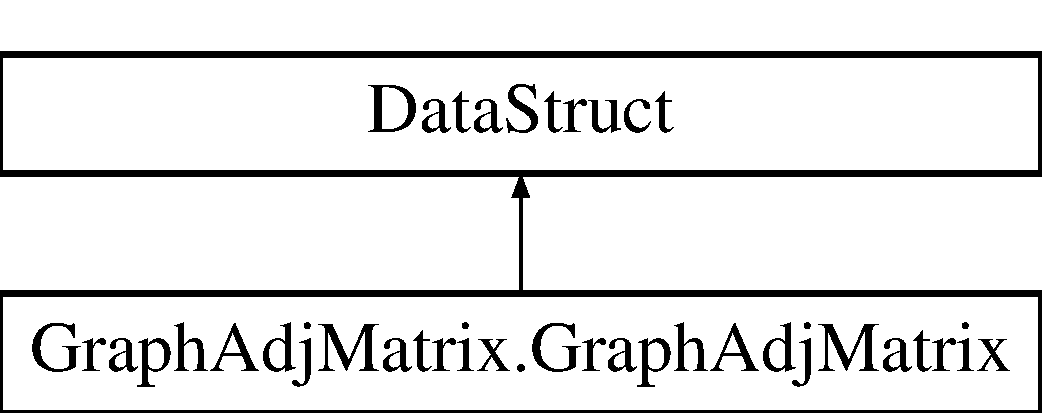
\includegraphics[height=2.000000cm]{class_graph_adj_matrix_1_1_graph_adj_matrix}
\end{center}
\end{figure}
\subsection*{Public Member Functions}
\begin{DoxyCompactItemize}
\item 
def \hyperlink{class_graph_adj_matrix_1_1_graph_adj_matrix_a18085a97b3716427398dfe0eb2e3db9f}{\+\_\+\+\_\+init\+\_\+\+\_\+} (self, size)
\begin{DoxyCompactList}\small\item\em Constructor. \end{DoxyCompactList}\item 
def \hyperlink{class_graph_adj_matrix_1_1_graph_adj_matrix_aa8d0e8805442fa980d2fa4ec07b29397}{get\+Data\+Struct\+Type} (self)
\begin{DoxyCompactList}\small\item\em This method gets the data structure type. \end{DoxyCompactList}\item 
def \hyperlink{class_graph_adj_matrix_1_1_graph_adj_matrix_a1439f978f7a9a362db75f1a0838783ad}{add\+Vertex} (self, k, e)
\begin{DoxyCompactList}\small\item\em Adds a new vertex to the graph, initializes the adjacency list; user is responsible for checking if the vertex already exists. \end{DoxyCompactList}\item 
def \hyperlink{class_graph_adj_matrix_1_1_graph_adj_matrix_ade007b6875b17bc0e56b08b27ab97de5}{add\+Edge} (self, src, dest)
\begin{DoxyCompactList}\small\item\em Adds a new edge to the graph, adds it to the index corresponding to the source, destination vertex ids; this version of the method assumes an edge weight of 1 (unweighted graph); user is responsible for checking if the vertices already exist, else an exception is thrown. \end{DoxyCompactList}\item 
def \hyperlink{class_graph_adj_matrix_1_1_graph_adj_matrix_aa1f4f5bcc4390fa3b28c5ff7d385c649}{add\+Edge\+\_\+0} (self, src, dest, weight)
\begin{DoxyCompactList}\small\item\em Adds a new edge of weight \textquotesingle{}weight\textquotesingle{} to the graph, adds it to the index corresponding to the source, destination vertex ids; user is responsible for checking if the vertices already exist, else an exception is thrown. \end{DoxyCompactList}\item 
def \hyperlink{class_graph_adj_matrix_1_1_graph_adj_matrix_aa3fbe3365150b94bdd232788defe7739}{get\+Vertices} (self)
\begin{DoxyCompactList}\small\item\em This method returns the graph nodes. \end{DoxyCompactList}\item 
def \hyperlink{class_graph_adj_matrix_1_1_graph_adj_matrix_ae5dc33de984eb621e610f1b79be6d65a}{get\+Adjacency\+Matrix} (self)
\begin{DoxyCompactList}\small\item\em Gets the adjacency matrix. \end{DoxyCompactList}\item 
def \hyperlink{class_graph_adj_matrix_1_1_graph_adj_matrix_a24dbf5218e61389b10fc969dcff5d7b0}{get\+Link\+Visualizer} (self, src, dest)
\begin{DoxyCompactList}\small\item\em This is a convenience method to simplify access to the link visualizer; the method assumes the vertex names point to existing vertices, else an exception is thrown. \end{DoxyCompactList}\item 
def \hyperlink{class_graph_adj_matrix_1_1_graph_adj_matrix_a17a86c39cd089c4a7379a47ffcff3390}{get\+Visualizer} (self, vertex)
\begin{DoxyCompactList}\small\item\em This is a convenience method to simplify access to the element visualizer; the method assumes the vertex name points to an existing vertice, else an exception is thrown. \end{DoxyCompactList}\item 
def \hyperlink{class_graph_adj_matrix_1_1_graph_adj_matrix_a1e44a6961936900a35b6e812940fbfa8}{get\+Data\+Structure\+Representation} (self)
\begin{DoxyCompactList}\small\item\em Get the J\+S\+ON representation of the the data structure. \end{DoxyCompactList}\end{DoxyCompactItemize}
\subsection*{Static Public Attributes}
\begin{DoxyCompactItemize}
\item 
\hyperlink{class_graph_adj_matrix_1_1_graph_adj_matrix_a45edf0723e51301b7789e92514d128f4}{max\+Size} = int()
\item 
\hyperlink{class_graph_adj_matrix_1_1_graph_adj_matrix_a85c454d09e82706b00563af339c0147f}{vertices} = Hash\+Map()
\item 
\hyperlink{class_graph_adj_matrix_1_1_graph_adj_matrix_aba658e4996d8a25b8c7260bb0f936ea7}{matrix} = Hash\+Map()
\end{DoxyCompactItemize}


\subsection{Detailed Description}
The \hyperlink{class_graph_adj_matrix_1_1_graph_adj_matrix}{Graph\+Adj\+Matrix} class can be used to represent adjacency matrix based graphs in B\+R\+I\+D\+G\+ES. 

The \hyperlink{class_graph_adj_matrix_1_1_graph_adj_matrix}{Graph\+Adj\+Matrix} class can be used to represent adjacency matrix based graphs in B\+R\+I\+D\+G\+ES; it takes 2 generic parameters\+: (1) K, which is an orderable key value used in accessing vertices (in constant time) using a hashmap. This permits data sets that need to be accessed by keys that are strings, and (2) E, an application defined type, and used in the \hyperlink{namespace_edge}{Edge} representation. The class is simply a wrapper around the Java Hashmap class and, thus, derives all its operations from it. B\+R\+I\+D\+G\+ES provides methods to visualize the graph and its contents.

The vertices of the graph are held in a Java hashmap, for near constant time access; this lets us use strings or integral ids for vertices. The edges are accessed by a second hashmap from each vertex, again assuring near constant access time. Each edge contains the terminating vertex id and weight, as defined by the \hyperlink{namespace_edge}{Edge} class structure.

Convenience methods are provided to add vertices and edges to the graph. Edges are retrieved by using the dual hashmap, given the vertex ids of the edge.

\begin{DoxyAuthor}{Author}
Kalpathi Subramanian, Mihai Mehedint
\end{DoxyAuthor}
\begin{DoxyDate}{Date}
7/12/15, 5/18/17
\end{DoxyDate}

\begin{DoxyParams}{Parameters}
{\em $<$\+E$>$} & application/user defined type used as part of vertices and edges \\
\hline
{\em $<$\+K$>$} & orderable key (string, int, etc) that is used to index into vertex structure, for fast access\\
\hline
\end{DoxyParams}
\begin{DoxySeeAlso}{See also}
Example tutorial at 
\end{DoxySeeAlso}
?? TO DO\begin{DoxyVerb}generated source for class GraphAdjMatrix \end{DoxyVerb}
 

\subsection{Constructor \& Destructor Documentation}
\hypertarget{class_graph_adj_matrix_1_1_graph_adj_matrix_a18085a97b3716427398dfe0eb2e3db9f}{}\label{class_graph_adj_matrix_1_1_graph_adj_matrix_a18085a97b3716427398dfe0eb2e3db9f} 
\index{Graph\+Adj\+Matrix\+::\+Graph\+Adj\+Matrix@{Graph\+Adj\+Matrix\+::\+Graph\+Adj\+Matrix}!\+\_\+\+\_\+init\+\_\+\+\_\+@{\+\_\+\+\_\+init\+\_\+\+\_\+}}
\index{\+\_\+\+\_\+init\+\_\+\+\_\+@{\+\_\+\+\_\+init\+\_\+\+\_\+}!Graph\+Adj\+Matrix\+::\+Graph\+Adj\+Matrix@{Graph\+Adj\+Matrix\+::\+Graph\+Adj\+Matrix}}
\subsubsection{\texorpdfstring{\+\_\+\+\_\+init\+\_\+\+\_\+()}{\_\_init\_\_()}}
{\footnotesize\ttfamily def Graph\+Adj\+Matrix.\+Graph\+Adj\+Matrix.\+\_\+\+\_\+init\+\_\+\+\_\+ (\begin{DoxyParamCaption}\item[{}]{self,  }\item[{}]{size }\end{DoxyParamCaption})}



Constructor. 

\begin{DoxyVerb}generated source for method __init__ \end{DoxyVerb}
 

\subsection{Member Function Documentation}
\hypertarget{class_graph_adj_matrix_1_1_graph_adj_matrix_ade007b6875b17bc0e56b08b27ab97de5}{}\label{class_graph_adj_matrix_1_1_graph_adj_matrix_ade007b6875b17bc0e56b08b27ab97de5} 
\index{Graph\+Adj\+Matrix\+::\+Graph\+Adj\+Matrix@{Graph\+Adj\+Matrix\+::\+Graph\+Adj\+Matrix}!add\+Edge@{add\+Edge}}
\index{add\+Edge@{add\+Edge}!Graph\+Adj\+Matrix\+::\+Graph\+Adj\+Matrix@{Graph\+Adj\+Matrix\+::\+Graph\+Adj\+Matrix}}
\subsubsection{\texorpdfstring{add\+Edge()}{addEdge()}}
{\footnotesize\ttfamily def Graph\+Adj\+Matrix.\+Graph\+Adj\+Matrix.\+add\+Edge (\begin{DoxyParamCaption}\item[{}]{self,  }\item[{}]{src,  }\item[{}]{dest }\end{DoxyParamCaption})}



Adds a new edge to the graph, adds it to the index corresponding to the source, destination vertex ids; this version of the method assumes an edge weight of 1 (unweighted graph); user is responsible for checking if the vertices already exist, else an exception is thrown. 


\begin{DoxyParams}{Parameters}
{\em src} & -\/ source vertex of edge \\
\hline
{\em dest} & -\/ destination vertex of edge\begin{DoxyVerb}generated source for method addEdge \end{DoxyVerb}
 \\
\hline
\end{DoxyParams}
\hypertarget{class_graph_adj_matrix_1_1_graph_adj_matrix_aa1f4f5bcc4390fa3b28c5ff7d385c649}{}\label{class_graph_adj_matrix_1_1_graph_adj_matrix_aa1f4f5bcc4390fa3b28c5ff7d385c649} 
\index{Graph\+Adj\+Matrix\+::\+Graph\+Adj\+Matrix@{Graph\+Adj\+Matrix\+::\+Graph\+Adj\+Matrix}!add\+Edge\+\_\+0@{add\+Edge\+\_\+0}}
\index{add\+Edge\+\_\+0@{add\+Edge\+\_\+0}!Graph\+Adj\+Matrix\+::\+Graph\+Adj\+Matrix@{Graph\+Adj\+Matrix\+::\+Graph\+Adj\+Matrix}}
\subsubsection{\texorpdfstring{add\+Edge\+\_\+0()}{addEdge\_0()}}
{\footnotesize\ttfamily def Graph\+Adj\+Matrix.\+Graph\+Adj\+Matrix.\+add\+Edge\+\_\+0 (\begin{DoxyParamCaption}\item[{}]{self,  }\item[{}]{src,  }\item[{}]{dest,  }\item[{}]{weight }\end{DoxyParamCaption})}



Adds a new edge of weight \textquotesingle{}weight\textquotesingle{} to the graph, adds it to the index corresponding to the source, destination vertex ids; user is responsible for checking if the vertices already exist, else an exception is thrown. 


\begin{DoxyParams}{Parameters}
{\em src} & -\/ source vertex of edge \\
\hline
{\em dest} & -\/ destination vertex of edge \\
\hline
{\em weight} & -\/ edge weight\begin{DoxyVerb}generated source for method addEdge_0 \end{DoxyVerb}
 \\
\hline
\end{DoxyParams}
\hypertarget{class_graph_adj_matrix_1_1_graph_adj_matrix_a1439f978f7a9a362db75f1a0838783ad}{}\label{class_graph_adj_matrix_1_1_graph_adj_matrix_a1439f978f7a9a362db75f1a0838783ad} 
\index{Graph\+Adj\+Matrix\+::\+Graph\+Adj\+Matrix@{Graph\+Adj\+Matrix\+::\+Graph\+Adj\+Matrix}!add\+Vertex@{add\+Vertex}}
\index{add\+Vertex@{add\+Vertex}!Graph\+Adj\+Matrix\+::\+Graph\+Adj\+Matrix@{Graph\+Adj\+Matrix\+::\+Graph\+Adj\+Matrix}}
\subsubsection{\texorpdfstring{add\+Vertex()}{addVertex()}}
{\footnotesize\ttfamily def Graph\+Adj\+Matrix.\+Graph\+Adj\+Matrix.\+add\+Vertex (\begin{DoxyParamCaption}\item[{}]{self,  }\item[{}]{k,  }\item[{}]{e }\end{DoxyParamCaption})}



Adds a new vertex to the graph, initializes the adjacency list; user is responsible for checking if the vertex already exists. 

This method will replace the value for this key


\begin{DoxyParams}{Parameters}
{\em k} & -\/ vertex key value \\
\hline
{\em 3} & -\/ user specified data, part of the vertex data\begin{DoxyVerb}generated source for method addVertex \end{DoxyVerb}
 \\
\hline
\end{DoxyParams}
\hypertarget{class_graph_adj_matrix_1_1_graph_adj_matrix_ae5dc33de984eb621e610f1b79be6d65a}{}\label{class_graph_adj_matrix_1_1_graph_adj_matrix_ae5dc33de984eb621e610f1b79be6d65a} 
\index{Graph\+Adj\+Matrix\+::\+Graph\+Adj\+Matrix@{Graph\+Adj\+Matrix\+::\+Graph\+Adj\+Matrix}!get\+Adjacency\+Matrix@{get\+Adjacency\+Matrix}}
\index{get\+Adjacency\+Matrix@{get\+Adjacency\+Matrix}!Graph\+Adj\+Matrix\+::\+Graph\+Adj\+Matrix@{Graph\+Adj\+Matrix\+::\+Graph\+Adj\+Matrix}}
\subsubsection{\texorpdfstring{get\+Adjacency\+Matrix()}{getAdjacencyMatrix()}}
{\footnotesize\ttfamily def Graph\+Adj\+Matrix.\+Graph\+Adj\+Matrix.\+get\+Adjacency\+Matrix (\begin{DoxyParamCaption}\item[{}]{self }\end{DoxyParamCaption})}



Gets the adjacency matrix. 

\begin{DoxyReturn}{Returns}
-\/ the graph\textquotesingle{}s adjacency matrix\begin{DoxyVerb}generated source for method getAdjacencyMatrix \end{DoxyVerb}
 
\end{DoxyReturn}
\hypertarget{class_graph_adj_matrix_1_1_graph_adj_matrix_aa8d0e8805442fa980d2fa4ec07b29397}{}\label{class_graph_adj_matrix_1_1_graph_adj_matrix_aa8d0e8805442fa980d2fa4ec07b29397} 
\index{Graph\+Adj\+Matrix\+::\+Graph\+Adj\+Matrix@{Graph\+Adj\+Matrix\+::\+Graph\+Adj\+Matrix}!get\+Data\+Struct\+Type@{get\+Data\+Struct\+Type}}
\index{get\+Data\+Struct\+Type@{get\+Data\+Struct\+Type}!Graph\+Adj\+Matrix\+::\+Graph\+Adj\+Matrix@{Graph\+Adj\+Matrix\+::\+Graph\+Adj\+Matrix}}
\subsubsection{\texorpdfstring{get\+Data\+Struct\+Type()}{getDataStructType()}}
{\footnotesize\ttfamily def Graph\+Adj\+Matrix.\+Graph\+Adj\+Matrix.\+get\+Data\+Struct\+Type (\begin{DoxyParamCaption}\item[{}]{self }\end{DoxyParamCaption})}



This method gets the data structure type. 

\begin{DoxyReturn}{Returns}
The date structure type as a string\begin{DoxyVerb}generated source for method getDataStructType \end{DoxyVerb}
 
\end{DoxyReturn}
\hypertarget{class_graph_adj_matrix_1_1_graph_adj_matrix_a1e44a6961936900a35b6e812940fbfa8}{}\label{class_graph_adj_matrix_1_1_graph_adj_matrix_a1e44a6961936900a35b6e812940fbfa8} 
\index{Graph\+Adj\+Matrix\+::\+Graph\+Adj\+Matrix@{Graph\+Adj\+Matrix\+::\+Graph\+Adj\+Matrix}!get\+Data\+Structure\+Representation@{get\+Data\+Structure\+Representation}}
\index{get\+Data\+Structure\+Representation@{get\+Data\+Structure\+Representation}!Graph\+Adj\+Matrix\+::\+Graph\+Adj\+Matrix@{Graph\+Adj\+Matrix\+::\+Graph\+Adj\+Matrix}}
\subsubsection{\texorpdfstring{get\+Data\+Structure\+Representation()}{getDataStructureRepresentation()}}
{\footnotesize\ttfamily def Graph\+Adj\+Matrix.\+Graph\+Adj\+Matrix.\+get\+Data\+Structure\+Representation (\begin{DoxyParamCaption}\item[{}]{self }\end{DoxyParamCaption})}



Get the J\+S\+ON representation of the the data structure. 

\begin{DoxyVerb}generated source for method getDataStructureRepresentation \end{DoxyVerb}
 \hypertarget{class_graph_adj_matrix_1_1_graph_adj_matrix_a24dbf5218e61389b10fc969dcff5d7b0}{}\label{class_graph_adj_matrix_1_1_graph_adj_matrix_a24dbf5218e61389b10fc969dcff5d7b0} 
\index{Graph\+Adj\+Matrix\+::\+Graph\+Adj\+Matrix@{Graph\+Adj\+Matrix\+::\+Graph\+Adj\+Matrix}!get\+Link\+Visualizer@{get\+Link\+Visualizer}}
\index{get\+Link\+Visualizer@{get\+Link\+Visualizer}!Graph\+Adj\+Matrix\+::\+Graph\+Adj\+Matrix@{Graph\+Adj\+Matrix\+::\+Graph\+Adj\+Matrix}}
\subsubsection{\texorpdfstring{get\+Link\+Visualizer()}{getLinkVisualizer()}}
{\footnotesize\ttfamily def Graph\+Adj\+Matrix.\+Graph\+Adj\+Matrix.\+get\+Link\+Visualizer (\begin{DoxyParamCaption}\item[{}]{self,  }\item[{}]{src,  }\item[{}]{dest }\end{DoxyParamCaption})}



This is a convenience method to simplify access to the link visualizer; the method assumes the vertex names point to existing vertices, else an exception is thrown. 

\begin{DoxyVerb}generated source for method getLinkVisualizer \end{DoxyVerb}
 \hypertarget{class_graph_adj_matrix_1_1_graph_adj_matrix_aa3fbe3365150b94bdd232788defe7739}{}\label{class_graph_adj_matrix_1_1_graph_adj_matrix_aa3fbe3365150b94bdd232788defe7739} 
\index{Graph\+Adj\+Matrix\+::\+Graph\+Adj\+Matrix@{Graph\+Adj\+Matrix\+::\+Graph\+Adj\+Matrix}!get\+Vertices@{get\+Vertices}}
\index{get\+Vertices@{get\+Vertices}!Graph\+Adj\+Matrix\+::\+Graph\+Adj\+Matrix@{Graph\+Adj\+Matrix\+::\+Graph\+Adj\+Matrix}}
\subsubsection{\texorpdfstring{get\+Vertices()}{getVertices()}}
{\footnotesize\ttfamily def Graph\+Adj\+Matrix.\+Graph\+Adj\+Matrix.\+get\+Vertices (\begin{DoxyParamCaption}\item[{}]{self }\end{DoxyParamCaption})}



This method returns the graph nodes. 

return -- vertices held in an unordered map\begin{DoxyVerb}generated source for method getVertices \end{DoxyVerb}
 \hypertarget{class_graph_adj_matrix_1_1_graph_adj_matrix_a17a86c39cd089c4a7379a47ffcff3390}{}\label{class_graph_adj_matrix_1_1_graph_adj_matrix_a17a86c39cd089c4a7379a47ffcff3390} 
\index{Graph\+Adj\+Matrix\+::\+Graph\+Adj\+Matrix@{Graph\+Adj\+Matrix\+::\+Graph\+Adj\+Matrix}!get\+Visualizer@{get\+Visualizer}}
\index{get\+Visualizer@{get\+Visualizer}!Graph\+Adj\+Matrix\+::\+Graph\+Adj\+Matrix@{Graph\+Adj\+Matrix\+::\+Graph\+Adj\+Matrix}}
\subsubsection{\texorpdfstring{get\+Visualizer()}{getVisualizer()}}
{\footnotesize\ttfamily def Graph\+Adj\+Matrix.\+Graph\+Adj\+Matrix.\+get\+Visualizer (\begin{DoxyParamCaption}\item[{}]{self,  }\item[{}]{vertex }\end{DoxyParamCaption})}



This is a convenience method to simplify access to the element visualizer; the method assumes the vertex name points to an existing vertice, else an exception is thrown. 

\begin{DoxyVerb}generated source for method getVisualizer \end{DoxyVerb}
 

\subsection{Member Data Documentation}
\hypertarget{class_graph_adj_matrix_1_1_graph_adj_matrix_aba658e4996d8a25b8c7260bb0f936ea7}{}\label{class_graph_adj_matrix_1_1_graph_adj_matrix_aba658e4996d8a25b8c7260bb0f936ea7} 
\index{Graph\+Adj\+Matrix\+::\+Graph\+Adj\+Matrix@{Graph\+Adj\+Matrix\+::\+Graph\+Adj\+Matrix}!matrix@{matrix}}
\index{matrix@{matrix}!Graph\+Adj\+Matrix\+::\+Graph\+Adj\+Matrix@{Graph\+Adj\+Matrix\+::\+Graph\+Adj\+Matrix}}
\subsubsection{\texorpdfstring{matrix}{matrix}}
{\footnotesize\ttfamily Graph\+Adj\+Matrix.\+Graph\+Adj\+Matrix.\+matrix = Hash\+Map()\hspace{0.3cm}{\ttfamily [static]}}

\hypertarget{class_graph_adj_matrix_1_1_graph_adj_matrix_a45edf0723e51301b7789e92514d128f4}{}\label{class_graph_adj_matrix_1_1_graph_adj_matrix_a45edf0723e51301b7789e92514d128f4} 
\index{Graph\+Adj\+Matrix\+::\+Graph\+Adj\+Matrix@{Graph\+Adj\+Matrix\+::\+Graph\+Adj\+Matrix}!max\+Size@{max\+Size}}
\index{max\+Size@{max\+Size}!Graph\+Adj\+Matrix\+::\+Graph\+Adj\+Matrix@{Graph\+Adj\+Matrix\+::\+Graph\+Adj\+Matrix}}
\subsubsection{\texorpdfstring{max\+Size}{maxSize}}
{\footnotesize\ttfamily Graph\+Adj\+Matrix.\+Graph\+Adj\+Matrix.\+max\+Size = int()\hspace{0.3cm}{\ttfamily [static]}}

\hypertarget{class_graph_adj_matrix_1_1_graph_adj_matrix_a85c454d09e82706b00563af339c0147f}{}\label{class_graph_adj_matrix_1_1_graph_adj_matrix_a85c454d09e82706b00563af339c0147f} 
\index{Graph\+Adj\+Matrix\+::\+Graph\+Adj\+Matrix@{Graph\+Adj\+Matrix\+::\+Graph\+Adj\+Matrix}!vertices@{vertices}}
\index{vertices@{vertices}!Graph\+Adj\+Matrix\+::\+Graph\+Adj\+Matrix@{Graph\+Adj\+Matrix\+::\+Graph\+Adj\+Matrix}}
\subsubsection{\texorpdfstring{vertices}{vertices}}
{\footnotesize\ttfamily Graph\+Adj\+Matrix.\+Graph\+Adj\+Matrix.\+vertices = Hash\+Map()\hspace{0.3cm}{\ttfamily [static]}}



The documentation for this class was generated from the following file\+:\begin{DoxyCompactItemize}
\item 
/\+Users/kalpathi/gr/bridges/client/python/src/\hyperlink{_graph_adj_matrix_8py}{Graph\+Adj\+Matrix.\+py}\end{DoxyCompactItemize}

\hypertarget{class_grid_1_1_grid}{}\section{Grid.\+Grid Class Reference}
\label{class_grid_1_1_grid}\index{Grid.\+Grid@{Grid.\+Grid}}
\subsection*{Public Member Functions}
\begin{DoxyCompactItemize}
\item 
def \hyperlink{class_grid_1_1_grid_aa5fda75ff87deb0bc314f46f37c32bbe}{get\+\_\+data\+\_\+structure\+\_\+type} (self)
\item 
def \hyperlink{class_grid_1_1_grid_ae7e2212c7a857bb888cf441095371e8a}{\+\_\+\+\_\+init\+\_\+\+\_\+} (self)
\item 
def \hyperlink{class_grid_1_1_grid_af5c7fb19e9c77314c07466fd2cae21fd}{get\+\_\+dimensions} (self)
\item 
def \hyperlink{class_grid_1_1_grid_a70d24548a9294179bf206f69cb6020fc}{get} (self, row, col)
\item 
def \hyperlink{class_grid_1_1_grid_aa796dcf3bd8872527537675a3691efc7}{set} (self, row, col, val)
\end{DoxyCompactItemize}
\subsection*{Public Attributes}
\begin{DoxyCompactItemize}
\item 
\hyperlink{class_grid_1_1_grid_ae40cd99c22229917de9d8809eb7c9a10}{grid}
\end{DoxyCompactItemize}
\subsection*{Static Public Attributes}
\begin{DoxyCompactItemize}
\item 
list \hyperlink{class_grid_1_1_grid_ada88ff869817a4d998885417f23abf37}{grid} = \mbox{[}$\,$\mbox{]}
\item 
list \hyperlink{class_grid_1_1_grid_a0e53d7466c48b288fb28deef2b870742}{grid\+Size} = \mbox{[}10, 10\mbox{]}
\item 
list \hyperlink{class_grid_1_1_grid_a4299841d081e91e31c4c86dc38bb7829}{max\+Grid\+Size} = \mbox{[}480, 640\mbox{]}
\end{DoxyCompactItemize}


\subsection{Constructor \& Destructor Documentation}
\hypertarget{class_grid_1_1_grid_ae7e2212c7a857bb888cf441095371e8a}{}\index{Grid\+::\+Grid@{Grid\+::\+Grid}!\+\_\+\+\_\+init\+\_\+\+\_\+@{\+\_\+\+\_\+init\+\_\+\+\_\+}}
\index{\+\_\+\+\_\+init\+\_\+\+\_\+@{\+\_\+\+\_\+init\+\_\+\+\_\+}!Grid\+::\+Grid@{Grid\+::\+Grid}}
\subsubsection[{\+\_\+\+\_\+init\+\_\+\+\_\+(self)}]{\setlength{\rightskip}{0pt plus 5cm}def Grid.\+Grid.\+\_\+\+\_\+init\+\_\+\+\_\+ (
\begin{DoxyParamCaption}
\item[{}]{self}
\end{DoxyParamCaption}
)}\label{class_grid_1_1_grid_ae7e2212c7a857bb888cf441095371e8a}


\subsection{Member Function Documentation}
\hypertarget{class_grid_1_1_grid_a70d24548a9294179bf206f69cb6020fc}{}\index{Grid\+::\+Grid@{Grid\+::\+Grid}!get@{get}}
\index{get@{get}!Grid\+::\+Grid@{Grid\+::\+Grid}}
\subsubsection[{get(self, row, col)}]{\setlength{\rightskip}{0pt plus 5cm}def Grid.\+Grid.\+get (
\begin{DoxyParamCaption}
\item[{}]{self, }
\item[{}]{row, }
\item[{}]{col}
\end{DoxyParamCaption}
)}\label{class_grid_1_1_grid_a70d24548a9294179bf206f69cb6020fc}
\hypertarget{class_grid_1_1_grid_aa5fda75ff87deb0bc314f46f37c32bbe}{}\index{Grid\+::\+Grid@{Grid\+::\+Grid}!get\+\_\+data\+\_\+structure\+\_\+type@{get\+\_\+data\+\_\+structure\+\_\+type}}
\index{get\+\_\+data\+\_\+structure\+\_\+type@{get\+\_\+data\+\_\+structure\+\_\+type}!Grid\+::\+Grid@{Grid\+::\+Grid}}
\subsubsection[{get\+\_\+data\+\_\+structure\+\_\+type(self)}]{\setlength{\rightskip}{0pt plus 5cm}def Grid.\+Grid.\+get\+\_\+data\+\_\+structure\+\_\+type (
\begin{DoxyParamCaption}
\item[{}]{self}
\end{DoxyParamCaption}
)}\label{class_grid_1_1_grid_aa5fda75ff87deb0bc314f46f37c32bbe}
\hypertarget{class_grid_1_1_grid_af5c7fb19e9c77314c07466fd2cae21fd}{}\index{Grid\+::\+Grid@{Grid\+::\+Grid}!get\+\_\+dimensions@{get\+\_\+dimensions}}
\index{get\+\_\+dimensions@{get\+\_\+dimensions}!Grid\+::\+Grid@{Grid\+::\+Grid}}
\subsubsection[{get\+\_\+dimensions(self)}]{\setlength{\rightskip}{0pt plus 5cm}def Grid.\+Grid.\+get\+\_\+dimensions (
\begin{DoxyParamCaption}
\item[{}]{self}
\end{DoxyParamCaption}
)}\label{class_grid_1_1_grid_af5c7fb19e9c77314c07466fd2cae21fd}
\hypertarget{class_grid_1_1_grid_aa796dcf3bd8872527537675a3691efc7}{}\index{Grid\+::\+Grid@{Grid\+::\+Grid}!set@{set}}
\index{set@{set}!Grid\+::\+Grid@{Grid\+::\+Grid}}
\subsubsection[{set(self, row, col, val)}]{\setlength{\rightskip}{0pt plus 5cm}def Grid.\+Grid.\+set (
\begin{DoxyParamCaption}
\item[{}]{self, }
\item[{}]{row, }
\item[{}]{col, }
\item[{}]{val}
\end{DoxyParamCaption}
)}\label{class_grid_1_1_grid_aa796dcf3bd8872527537675a3691efc7}


\subsection{Member Data Documentation}
\hypertarget{class_grid_1_1_grid_ada88ff869817a4d998885417f23abf37}{}\index{Grid\+::\+Grid@{Grid\+::\+Grid}!grid@{grid}}
\index{grid@{grid}!Grid\+::\+Grid@{Grid\+::\+Grid}}
\subsubsection[{grid}]{\setlength{\rightskip}{0pt plus 5cm}list Grid.\+Grid.\+grid = \mbox{[}$\,$\mbox{]}\hspace{0.3cm}{\ttfamily [static]}}\label{class_grid_1_1_grid_ada88ff869817a4d998885417f23abf37}
\hypertarget{class_grid_1_1_grid_ae40cd99c22229917de9d8809eb7c9a10}{}\index{Grid\+::\+Grid@{Grid\+::\+Grid}!grid@{grid}}
\index{grid@{grid}!Grid\+::\+Grid@{Grid\+::\+Grid}}
\subsubsection[{grid}]{\setlength{\rightskip}{0pt plus 5cm}Grid.\+Grid.\+grid}\label{class_grid_1_1_grid_ae40cd99c22229917de9d8809eb7c9a10}
\hypertarget{class_grid_1_1_grid_a0e53d7466c48b288fb28deef2b870742}{}\index{Grid\+::\+Grid@{Grid\+::\+Grid}!grid\+Size@{grid\+Size}}
\index{grid\+Size@{grid\+Size}!Grid\+::\+Grid@{Grid\+::\+Grid}}
\subsubsection[{grid\+Size}]{\setlength{\rightskip}{0pt plus 5cm}list Grid.\+Grid.\+grid\+Size = \mbox{[}10, 10\mbox{]}\hspace{0.3cm}{\ttfamily [static]}}\label{class_grid_1_1_grid_a0e53d7466c48b288fb28deef2b870742}
\hypertarget{class_grid_1_1_grid_a4299841d081e91e31c4c86dc38bb7829}{}\index{Grid\+::\+Grid@{Grid\+::\+Grid}!max\+Grid\+Size@{max\+Grid\+Size}}
\index{max\+Grid\+Size@{max\+Grid\+Size}!Grid\+::\+Grid@{Grid\+::\+Grid}}
\subsubsection[{max\+Grid\+Size}]{\setlength{\rightskip}{0pt plus 5cm}list Grid.\+Grid.\+max\+Grid\+Size = \mbox{[}480, 640\mbox{]}\hspace{0.3cm}{\ttfamily [static]}}\label{class_grid_1_1_grid_a4299841d081e91e31c4c86dc38bb7829}


The documentation for this class was generated from the following file\+:\begin{DoxyCompactItemize}
\item 
/\+Users/krs/gr/bridges/bridges17/python/src/\hyperlink{_grid_8py}{Grid.\+py}\end{DoxyCompactItemize}

\hypertarget{class_gutenberg_book_1_1_gutenberg_book}{}\section{Gutenberg\+Book.\+Gutenberg\+Book Class Reference}
\label{class_gutenberg_book_1_1_gutenberg_book}\index{Gutenberg\+Book.\+Gutenberg\+Book@{Gutenberg\+Book.\+Gutenberg\+Book}}
\subsection*{Public Member Functions}
\begin{DoxyCompactItemize}
\item 
def \hyperlink{class_gutenberg_book_1_1_gutenberg_book_ab54eccb3d7735821ded27353cc967139}{\+\_\+\+\_\+init\+\_\+\+\_\+}
\item 
def \hyperlink{class_gutenberg_book_1_1_gutenberg_book_af373b71a5b05dab220647c2d32ff4bce}{get\+Author\+Name} (self)
\item 
def \hyperlink{class_gutenberg_book_1_1_gutenberg_book_a08b7d5550df691a9dbd2b8341df1c199}{set\+Author\+Name} (self, \hyperlink{class_gutenberg_book_1_1_gutenberg_book_aa791b333bc15083ffcd70e31565c3ce0}{author\+Name})
\item 
def \hyperlink{class_gutenberg_book_1_1_gutenberg_book_a8f2e41009352ef78ffa96aa693ea0a27}{get\+Author\+Birth} (self)
\item 
def \hyperlink{class_gutenberg_book_1_1_gutenberg_book_ac379f43783f7f3db54a44635cbe0a465}{set\+Authro\+Birth} (self, \hyperlink{class_gutenberg_book_1_1_gutenberg_book_aa470512f70b49c44577cda4167a2abe4}{author\+Birth})
\item 
def \hyperlink{class_gutenberg_book_1_1_gutenberg_book_a65d075fb4340f1b942416134bc3ae426}{get\+Author\+Death} (self)
\item 
def \hyperlink{class_gutenberg_book_1_1_gutenberg_book_a8872fe6b29888ad3122748a0a87f4b66}{set\+Author\+Death} (self, \hyperlink{class_gutenberg_book_1_1_gutenberg_book_a271f557aa0ed0b5a1430b7250e5c6da9}{author\+Death})
\item 
def \hyperlink{class_gutenberg_book_1_1_gutenberg_book_ae12a0d74064224aa20921cff74cf1f02}{get\+Title} (self)
\item 
def \hyperlink{class_gutenberg_book_1_1_gutenberg_book_a41daad48dbcf32d8ed7918092295c7f0}{set\+Title} (self, \hyperlink{class_gutenberg_book_1_1_gutenberg_book_adbf667fb4a34b8937c3c4e755f62b3dd}{title})
\item 
def \hyperlink{class_gutenberg_book_1_1_gutenberg_book_ab0456baf3ba5650c8ca5d1340c0aa53b}{get\+Genre} (self)
\item 
def \hyperlink{class_gutenberg_book_1_1_gutenberg_book_a9fb7a7667deda6077c7442a6437a0783}{set\+Genre} (self, \hyperlink{class_gutenberg_book_1_1_gutenberg_book_ab26f43198c585ea7b4b1413250e75d78}{genre})
\item 
def \hyperlink{class_gutenberg_book_1_1_gutenberg_book_a32d638f7891d61aae4fabd2e1940d8a2}{get\+Subject} (self)
\item 
def \hyperlink{class_gutenberg_book_1_1_gutenberg_book_a110d79b5d2f57700935f95609b7192cf}{set\+Subject} (self, \hyperlink{class_gutenberg_book_1_1_gutenberg_book_ae8cefa9cabbbbe09e919b9c0e8f6577e}{subject})
\item 
def \hyperlink{class_gutenberg_book_1_1_gutenberg_book_af3311d3f4c1a2f16fd13a91b2a64ef44}{get\+Num\+Words} (self)
\item 
def \hyperlink{class_gutenberg_book_1_1_gutenberg_book_a02e3c8a8c2219d9120a86cea7b7902a4}{set\+Num\+Words} (self, \hyperlink{class_gutenberg_book_1_1_gutenberg_book_a03bded71365c803889b37370001bc679}{num\+Words})
\item 
def \hyperlink{class_gutenberg_book_1_1_gutenberg_book_a778b3437a11a6884c505b71ead63a074}{get\+Num\+Sentences} (self)
\item 
def \hyperlink{class_gutenberg_book_1_1_gutenberg_book_a1b335a4ce7484b547b7acf5a8c86e591}{set\+Nume\+Sentences} (self, \hyperlink{class_gutenberg_book_1_1_gutenberg_book_ae2b9fe952d14c8193d95f5ed2a51e679}{num\+Sentences})
\item 
def \hyperlink{class_gutenberg_book_1_1_gutenberg_book_a2a9cd21224d17e5da28889751529c31c}{get\+Num\+Difficult\+Words} (self)
\item 
def \hyperlink{class_gutenberg_book_1_1_gutenberg_book_a9c0c61e2580f8008656dafa8811be96d}{set\+Num\+Difficult\+Words} (self, \hyperlink{class_gutenberg_book_1_1_gutenberg_book_a702230ada41f3fbf9daa27234893c8d7}{num\+Difficult\+Words})
\end{DoxyCompactItemize}
\subsection*{Public Attributes}
\begin{DoxyCompactItemize}
\item 
\hyperlink{class_gutenberg_book_1_1_gutenberg_book_aa791b333bc15083ffcd70e31565c3ce0}{author\+Name}
\item 
\hyperlink{class_gutenberg_book_1_1_gutenberg_book_aa470512f70b49c44577cda4167a2abe4}{author\+Birth}
\item 
\hyperlink{class_gutenberg_book_1_1_gutenberg_book_a271f557aa0ed0b5a1430b7250e5c6da9}{author\+Death}
\item 
\hyperlink{class_gutenberg_book_1_1_gutenberg_book_adbf667fb4a34b8937c3c4e755f62b3dd}{title}
\item 
\hyperlink{class_gutenberg_book_1_1_gutenberg_book_a4186b4fde315e2e55f3d9833a620c952}{lang}
\item 
\hyperlink{class_gutenberg_book_1_1_gutenberg_book_ab26f43198c585ea7b4b1413250e75d78}{genre}
\item 
\hyperlink{class_gutenberg_book_1_1_gutenberg_book_ae8cefa9cabbbbe09e919b9c0e8f6577e}{subject}
\item 
\hyperlink{class_gutenberg_book_1_1_gutenberg_book_a8d0bd46f760033b5ddc164d74c5f9f41}{num\+Chars}
\item 
\hyperlink{class_gutenberg_book_1_1_gutenberg_book_a03bded71365c803889b37370001bc679}{num\+Words}
\item 
\hyperlink{class_gutenberg_book_1_1_gutenberg_book_ae2b9fe952d14c8193d95f5ed2a51e679}{num\+Sentences}
\item 
\hyperlink{class_gutenberg_book_1_1_gutenberg_book_a702230ada41f3fbf9daa27234893c8d7}{num\+Difficult\+Words}
\item 
\hyperlink{class_gutenberg_book_1_1_gutenberg_book_a1b1ef102b505b472d010795193a1594c}{url}
\end{DoxyCompactItemize}


\subsection{Constructor \& Destructor Documentation}
\hypertarget{class_gutenberg_book_1_1_gutenberg_book_ab54eccb3d7735821ded27353cc967139}{}\index{Gutenberg\+Book\+::\+Gutenberg\+Book@{Gutenberg\+Book\+::\+Gutenberg\+Book}!\+\_\+\+\_\+init\+\_\+\+\_\+@{\+\_\+\+\_\+init\+\_\+\+\_\+}}
\index{\+\_\+\+\_\+init\+\_\+\+\_\+@{\+\_\+\+\_\+init\+\_\+\+\_\+}!Gutenberg\+Book\+::\+Gutenberg\+Book@{Gutenberg\+Book\+::\+Gutenberg\+Book}}
\subsubsection[{\+\_\+\+\_\+init\+\_\+\+\_\+}]{\setlength{\rightskip}{0pt plus 5cm}def Gutenberg\+Book.\+Gutenberg\+Book.\+\_\+\+\_\+init\+\_\+\+\_\+ (
\begin{DoxyParamCaption}
\item[{}]{self, }
\item[{}]{author\+Name = {\ttfamily None}, }
\item[{}]{author\+Birth = {\ttfamily None}, }
\item[{}]{author\+Death = {\ttfamily None}, }
\item[{}]{title = {\ttfamily None}, }
\item[{}]{lang = {\ttfamily None}, }
\item[{}]{genre = {\ttfamily None}, }
\item[{}]{subject = {\ttfamily None}, }
\item[{}]{num\+Chars = {\ttfamily None}, }
\item[{}]{num\+Words = {\ttfamily None}, }
\item[{}]{num\+Sentences = {\ttfamily None}, }
\item[{}]{num\+Difficult\+Words = {\ttfamily None}, }
\item[{}]{url = {\ttfamily None}, }
\item[{}]{downloads = {\ttfamily None}}
\end{DoxyParamCaption}
)}\label{class_gutenberg_book_1_1_gutenberg_book_ab54eccb3d7735821ded27353cc967139}


\subsection{Member Function Documentation}
\hypertarget{class_gutenberg_book_1_1_gutenberg_book_a8f2e41009352ef78ffa96aa693ea0a27}{}\index{Gutenberg\+Book\+::\+Gutenberg\+Book@{Gutenberg\+Book\+::\+Gutenberg\+Book}!get\+Author\+Birth@{get\+Author\+Birth}}
\index{get\+Author\+Birth@{get\+Author\+Birth}!Gutenberg\+Book\+::\+Gutenberg\+Book@{Gutenberg\+Book\+::\+Gutenberg\+Book}}
\subsubsection[{get\+Author\+Birth(self)}]{\setlength{\rightskip}{0pt plus 5cm}def Gutenberg\+Book.\+Gutenberg\+Book.\+get\+Author\+Birth (
\begin{DoxyParamCaption}
\item[{}]{self}
\end{DoxyParamCaption}
)}\label{class_gutenberg_book_1_1_gutenberg_book_a8f2e41009352ef78ffa96aa693ea0a27}
\hypertarget{class_gutenberg_book_1_1_gutenberg_book_a65d075fb4340f1b942416134bc3ae426}{}\index{Gutenberg\+Book\+::\+Gutenberg\+Book@{Gutenberg\+Book\+::\+Gutenberg\+Book}!get\+Author\+Death@{get\+Author\+Death}}
\index{get\+Author\+Death@{get\+Author\+Death}!Gutenberg\+Book\+::\+Gutenberg\+Book@{Gutenberg\+Book\+::\+Gutenberg\+Book}}
\subsubsection[{get\+Author\+Death(self)}]{\setlength{\rightskip}{0pt plus 5cm}def Gutenberg\+Book.\+Gutenberg\+Book.\+get\+Author\+Death (
\begin{DoxyParamCaption}
\item[{}]{self}
\end{DoxyParamCaption}
)}\label{class_gutenberg_book_1_1_gutenberg_book_a65d075fb4340f1b942416134bc3ae426}
\hypertarget{class_gutenberg_book_1_1_gutenberg_book_af373b71a5b05dab220647c2d32ff4bce}{}\index{Gutenberg\+Book\+::\+Gutenberg\+Book@{Gutenberg\+Book\+::\+Gutenberg\+Book}!get\+Author\+Name@{get\+Author\+Name}}
\index{get\+Author\+Name@{get\+Author\+Name}!Gutenberg\+Book\+::\+Gutenberg\+Book@{Gutenberg\+Book\+::\+Gutenberg\+Book}}
\subsubsection[{get\+Author\+Name(self)}]{\setlength{\rightskip}{0pt plus 5cm}def Gutenberg\+Book.\+Gutenberg\+Book.\+get\+Author\+Name (
\begin{DoxyParamCaption}
\item[{}]{self}
\end{DoxyParamCaption}
)}\label{class_gutenberg_book_1_1_gutenberg_book_af373b71a5b05dab220647c2d32ff4bce}
\hypertarget{class_gutenberg_book_1_1_gutenberg_book_ab0456baf3ba5650c8ca5d1340c0aa53b}{}\index{Gutenberg\+Book\+::\+Gutenberg\+Book@{Gutenberg\+Book\+::\+Gutenberg\+Book}!get\+Genre@{get\+Genre}}
\index{get\+Genre@{get\+Genre}!Gutenberg\+Book\+::\+Gutenberg\+Book@{Gutenberg\+Book\+::\+Gutenberg\+Book}}
\subsubsection[{get\+Genre(self)}]{\setlength{\rightskip}{0pt plus 5cm}def Gutenberg\+Book.\+Gutenberg\+Book.\+get\+Genre (
\begin{DoxyParamCaption}
\item[{}]{self}
\end{DoxyParamCaption}
)}\label{class_gutenberg_book_1_1_gutenberg_book_ab0456baf3ba5650c8ca5d1340c0aa53b}
\hypertarget{class_gutenberg_book_1_1_gutenberg_book_a2a9cd21224d17e5da28889751529c31c}{}\index{Gutenberg\+Book\+::\+Gutenberg\+Book@{Gutenberg\+Book\+::\+Gutenberg\+Book}!get\+Num\+Difficult\+Words@{get\+Num\+Difficult\+Words}}
\index{get\+Num\+Difficult\+Words@{get\+Num\+Difficult\+Words}!Gutenberg\+Book\+::\+Gutenberg\+Book@{Gutenberg\+Book\+::\+Gutenberg\+Book}}
\subsubsection[{get\+Num\+Difficult\+Words(self)}]{\setlength{\rightskip}{0pt plus 5cm}def Gutenberg\+Book.\+Gutenberg\+Book.\+get\+Num\+Difficult\+Words (
\begin{DoxyParamCaption}
\item[{}]{self}
\end{DoxyParamCaption}
)}\label{class_gutenberg_book_1_1_gutenberg_book_a2a9cd21224d17e5da28889751529c31c}
\hypertarget{class_gutenberg_book_1_1_gutenberg_book_a778b3437a11a6884c505b71ead63a074}{}\index{Gutenberg\+Book\+::\+Gutenberg\+Book@{Gutenberg\+Book\+::\+Gutenberg\+Book}!get\+Num\+Sentences@{get\+Num\+Sentences}}
\index{get\+Num\+Sentences@{get\+Num\+Sentences}!Gutenberg\+Book\+::\+Gutenberg\+Book@{Gutenberg\+Book\+::\+Gutenberg\+Book}}
\subsubsection[{get\+Num\+Sentences(self)}]{\setlength{\rightskip}{0pt plus 5cm}def Gutenberg\+Book.\+Gutenberg\+Book.\+get\+Num\+Sentences (
\begin{DoxyParamCaption}
\item[{}]{self}
\end{DoxyParamCaption}
)}\label{class_gutenberg_book_1_1_gutenberg_book_a778b3437a11a6884c505b71ead63a074}
\hypertarget{class_gutenberg_book_1_1_gutenberg_book_af3311d3f4c1a2f16fd13a91b2a64ef44}{}\index{Gutenberg\+Book\+::\+Gutenberg\+Book@{Gutenberg\+Book\+::\+Gutenberg\+Book}!get\+Num\+Words@{get\+Num\+Words}}
\index{get\+Num\+Words@{get\+Num\+Words}!Gutenberg\+Book\+::\+Gutenberg\+Book@{Gutenberg\+Book\+::\+Gutenberg\+Book}}
\subsubsection[{get\+Num\+Words(self)}]{\setlength{\rightskip}{0pt plus 5cm}def Gutenberg\+Book.\+Gutenberg\+Book.\+get\+Num\+Words (
\begin{DoxyParamCaption}
\item[{}]{self}
\end{DoxyParamCaption}
)}\label{class_gutenberg_book_1_1_gutenberg_book_af3311d3f4c1a2f16fd13a91b2a64ef44}
\hypertarget{class_gutenberg_book_1_1_gutenberg_book_a32d638f7891d61aae4fabd2e1940d8a2}{}\index{Gutenberg\+Book\+::\+Gutenberg\+Book@{Gutenberg\+Book\+::\+Gutenberg\+Book}!get\+Subject@{get\+Subject}}
\index{get\+Subject@{get\+Subject}!Gutenberg\+Book\+::\+Gutenberg\+Book@{Gutenberg\+Book\+::\+Gutenberg\+Book}}
\subsubsection[{get\+Subject(self)}]{\setlength{\rightskip}{0pt plus 5cm}def Gutenberg\+Book.\+Gutenberg\+Book.\+get\+Subject (
\begin{DoxyParamCaption}
\item[{}]{self}
\end{DoxyParamCaption}
)}\label{class_gutenberg_book_1_1_gutenberg_book_a32d638f7891d61aae4fabd2e1940d8a2}
\hypertarget{class_gutenberg_book_1_1_gutenberg_book_ae12a0d74064224aa20921cff74cf1f02}{}\index{Gutenberg\+Book\+::\+Gutenberg\+Book@{Gutenberg\+Book\+::\+Gutenberg\+Book}!get\+Title@{get\+Title}}
\index{get\+Title@{get\+Title}!Gutenberg\+Book\+::\+Gutenberg\+Book@{Gutenberg\+Book\+::\+Gutenberg\+Book}}
\subsubsection[{get\+Title(self)}]{\setlength{\rightskip}{0pt plus 5cm}def Gutenberg\+Book.\+Gutenberg\+Book.\+get\+Title (
\begin{DoxyParamCaption}
\item[{}]{self}
\end{DoxyParamCaption}
)}\label{class_gutenberg_book_1_1_gutenberg_book_ae12a0d74064224aa20921cff74cf1f02}
\hypertarget{class_gutenberg_book_1_1_gutenberg_book_a8872fe6b29888ad3122748a0a87f4b66}{}\index{Gutenberg\+Book\+::\+Gutenberg\+Book@{Gutenberg\+Book\+::\+Gutenberg\+Book}!set\+Author\+Death@{set\+Author\+Death}}
\index{set\+Author\+Death@{set\+Author\+Death}!Gutenberg\+Book\+::\+Gutenberg\+Book@{Gutenberg\+Book\+::\+Gutenberg\+Book}}
\subsubsection[{set\+Author\+Death(self, author\+Death)}]{\setlength{\rightskip}{0pt plus 5cm}def Gutenberg\+Book.\+Gutenberg\+Book.\+set\+Author\+Death (
\begin{DoxyParamCaption}
\item[{}]{self, }
\item[{}]{author\+Death}
\end{DoxyParamCaption}
)}\label{class_gutenberg_book_1_1_gutenberg_book_a8872fe6b29888ad3122748a0a87f4b66}
\hypertarget{class_gutenberg_book_1_1_gutenberg_book_a08b7d5550df691a9dbd2b8341df1c199}{}\index{Gutenberg\+Book\+::\+Gutenberg\+Book@{Gutenberg\+Book\+::\+Gutenberg\+Book}!set\+Author\+Name@{set\+Author\+Name}}
\index{set\+Author\+Name@{set\+Author\+Name}!Gutenberg\+Book\+::\+Gutenberg\+Book@{Gutenberg\+Book\+::\+Gutenberg\+Book}}
\subsubsection[{set\+Author\+Name(self, author\+Name)}]{\setlength{\rightskip}{0pt plus 5cm}def Gutenberg\+Book.\+Gutenberg\+Book.\+set\+Author\+Name (
\begin{DoxyParamCaption}
\item[{}]{self, }
\item[{}]{author\+Name}
\end{DoxyParamCaption}
)}\label{class_gutenberg_book_1_1_gutenberg_book_a08b7d5550df691a9dbd2b8341df1c199}
\hypertarget{class_gutenberg_book_1_1_gutenberg_book_ac379f43783f7f3db54a44635cbe0a465}{}\index{Gutenberg\+Book\+::\+Gutenberg\+Book@{Gutenberg\+Book\+::\+Gutenberg\+Book}!set\+Authro\+Birth@{set\+Authro\+Birth}}
\index{set\+Authro\+Birth@{set\+Authro\+Birth}!Gutenberg\+Book\+::\+Gutenberg\+Book@{Gutenberg\+Book\+::\+Gutenberg\+Book}}
\subsubsection[{set\+Authro\+Birth(self, author\+Birth)}]{\setlength{\rightskip}{0pt plus 5cm}def Gutenberg\+Book.\+Gutenberg\+Book.\+set\+Authro\+Birth (
\begin{DoxyParamCaption}
\item[{}]{self, }
\item[{}]{author\+Birth}
\end{DoxyParamCaption}
)}\label{class_gutenberg_book_1_1_gutenberg_book_ac379f43783f7f3db54a44635cbe0a465}
\hypertarget{class_gutenberg_book_1_1_gutenberg_book_a9fb7a7667deda6077c7442a6437a0783}{}\index{Gutenberg\+Book\+::\+Gutenberg\+Book@{Gutenberg\+Book\+::\+Gutenberg\+Book}!set\+Genre@{set\+Genre}}
\index{set\+Genre@{set\+Genre}!Gutenberg\+Book\+::\+Gutenberg\+Book@{Gutenberg\+Book\+::\+Gutenberg\+Book}}
\subsubsection[{set\+Genre(self, genre)}]{\setlength{\rightskip}{0pt plus 5cm}def Gutenberg\+Book.\+Gutenberg\+Book.\+set\+Genre (
\begin{DoxyParamCaption}
\item[{}]{self, }
\item[{}]{genre}
\end{DoxyParamCaption}
)}\label{class_gutenberg_book_1_1_gutenberg_book_a9fb7a7667deda6077c7442a6437a0783}
\hypertarget{class_gutenberg_book_1_1_gutenberg_book_a9c0c61e2580f8008656dafa8811be96d}{}\index{Gutenberg\+Book\+::\+Gutenberg\+Book@{Gutenberg\+Book\+::\+Gutenberg\+Book}!set\+Num\+Difficult\+Words@{set\+Num\+Difficult\+Words}}
\index{set\+Num\+Difficult\+Words@{set\+Num\+Difficult\+Words}!Gutenberg\+Book\+::\+Gutenberg\+Book@{Gutenberg\+Book\+::\+Gutenberg\+Book}}
\subsubsection[{set\+Num\+Difficult\+Words(self, num\+Difficult\+Words)}]{\setlength{\rightskip}{0pt plus 5cm}def Gutenberg\+Book.\+Gutenberg\+Book.\+set\+Num\+Difficult\+Words (
\begin{DoxyParamCaption}
\item[{}]{self, }
\item[{}]{num\+Difficult\+Words}
\end{DoxyParamCaption}
)}\label{class_gutenberg_book_1_1_gutenberg_book_a9c0c61e2580f8008656dafa8811be96d}
\hypertarget{class_gutenberg_book_1_1_gutenberg_book_a1b335a4ce7484b547b7acf5a8c86e591}{}\index{Gutenberg\+Book\+::\+Gutenberg\+Book@{Gutenberg\+Book\+::\+Gutenberg\+Book}!set\+Nume\+Sentences@{set\+Nume\+Sentences}}
\index{set\+Nume\+Sentences@{set\+Nume\+Sentences}!Gutenberg\+Book\+::\+Gutenberg\+Book@{Gutenberg\+Book\+::\+Gutenberg\+Book}}
\subsubsection[{set\+Nume\+Sentences(self, num\+Sentences)}]{\setlength{\rightskip}{0pt plus 5cm}def Gutenberg\+Book.\+Gutenberg\+Book.\+set\+Nume\+Sentences (
\begin{DoxyParamCaption}
\item[{}]{self, }
\item[{}]{num\+Sentences}
\end{DoxyParamCaption}
)}\label{class_gutenberg_book_1_1_gutenberg_book_a1b335a4ce7484b547b7acf5a8c86e591}
\hypertarget{class_gutenberg_book_1_1_gutenberg_book_a02e3c8a8c2219d9120a86cea7b7902a4}{}\index{Gutenberg\+Book\+::\+Gutenberg\+Book@{Gutenberg\+Book\+::\+Gutenberg\+Book}!set\+Num\+Words@{set\+Num\+Words}}
\index{set\+Num\+Words@{set\+Num\+Words}!Gutenberg\+Book\+::\+Gutenberg\+Book@{Gutenberg\+Book\+::\+Gutenberg\+Book}}
\subsubsection[{set\+Num\+Words(self, num\+Words)}]{\setlength{\rightskip}{0pt plus 5cm}def Gutenberg\+Book.\+Gutenberg\+Book.\+set\+Num\+Words (
\begin{DoxyParamCaption}
\item[{}]{self, }
\item[{}]{num\+Words}
\end{DoxyParamCaption}
)}\label{class_gutenberg_book_1_1_gutenberg_book_a02e3c8a8c2219d9120a86cea7b7902a4}
\hypertarget{class_gutenberg_book_1_1_gutenberg_book_a110d79b5d2f57700935f95609b7192cf}{}\index{Gutenberg\+Book\+::\+Gutenberg\+Book@{Gutenberg\+Book\+::\+Gutenberg\+Book}!set\+Subject@{set\+Subject}}
\index{set\+Subject@{set\+Subject}!Gutenberg\+Book\+::\+Gutenberg\+Book@{Gutenberg\+Book\+::\+Gutenberg\+Book}}
\subsubsection[{set\+Subject(self, subject)}]{\setlength{\rightskip}{0pt plus 5cm}def Gutenberg\+Book.\+Gutenberg\+Book.\+set\+Subject (
\begin{DoxyParamCaption}
\item[{}]{self, }
\item[{}]{subject}
\end{DoxyParamCaption}
)}\label{class_gutenberg_book_1_1_gutenberg_book_a110d79b5d2f57700935f95609b7192cf}
\hypertarget{class_gutenberg_book_1_1_gutenberg_book_a41daad48dbcf32d8ed7918092295c7f0}{}\index{Gutenberg\+Book\+::\+Gutenberg\+Book@{Gutenberg\+Book\+::\+Gutenberg\+Book}!set\+Title@{set\+Title}}
\index{set\+Title@{set\+Title}!Gutenberg\+Book\+::\+Gutenberg\+Book@{Gutenberg\+Book\+::\+Gutenberg\+Book}}
\subsubsection[{set\+Title(self, title)}]{\setlength{\rightskip}{0pt plus 5cm}def Gutenberg\+Book.\+Gutenberg\+Book.\+set\+Title (
\begin{DoxyParamCaption}
\item[{}]{self, }
\item[{}]{title}
\end{DoxyParamCaption}
)}\label{class_gutenberg_book_1_1_gutenberg_book_a41daad48dbcf32d8ed7918092295c7f0}


\subsection{Member Data Documentation}
\hypertarget{class_gutenberg_book_1_1_gutenberg_book_aa470512f70b49c44577cda4167a2abe4}{}\index{Gutenberg\+Book\+::\+Gutenberg\+Book@{Gutenberg\+Book\+::\+Gutenberg\+Book}!author\+Birth@{author\+Birth}}
\index{author\+Birth@{author\+Birth}!Gutenberg\+Book\+::\+Gutenberg\+Book@{Gutenberg\+Book\+::\+Gutenberg\+Book}}
\subsubsection[{author\+Birth}]{\setlength{\rightskip}{0pt plus 5cm}Gutenberg\+Book.\+Gutenberg\+Book.\+author\+Birth}\label{class_gutenberg_book_1_1_gutenberg_book_aa470512f70b49c44577cda4167a2abe4}
\hypertarget{class_gutenberg_book_1_1_gutenberg_book_a271f557aa0ed0b5a1430b7250e5c6da9}{}\index{Gutenberg\+Book\+::\+Gutenberg\+Book@{Gutenberg\+Book\+::\+Gutenberg\+Book}!author\+Death@{author\+Death}}
\index{author\+Death@{author\+Death}!Gutenberg\+Book\+::\+Gutenberg\+Book@{Gutenberg\+Book\+::\+Gutenberg\+Book}}
\subsubsection[{author\+Death}]{\setlength{\rightskip}{0pt plus 5cm}Gutenberg\+Book.\+Gutenberg\+Book.\+author\+Death}\label{class_gutenberg_book_1_1_gutenberg_book_a271f557aa0ed0b5a1430b7250e5c6da9}
\hypertarget{class_gutenberg_book_1_1_gutenberg_book_aa791b333bc15083ffcd70e31565c3ce0}{}\index{Gutenberg\+Book\+::\+Gutenberg\+Book@{Gutenberg\+Book\+::\+Gutenberg\+Book}!author\+Name@{author\+Name}}
\index{author\+Name@{author\+Name}!Gutenberg\+Book\+::\+Gutenberg\+Book@{Gutenberg\+Book\+::\+Gutenberg\+Book}}
\subsubsection[{author\+Name}]{\setlength{\rightskip}{0pt plus 5cm}Gutenberg\+Book.\+Gutenberg\+Book.\+author\+Name}\label{class_gutenberg_book_1_1_gutenberg_book_aa791b333bc15083ffcd70e31565c3ce0}
\hypertarget{class_gutenberg_book_1_1_gutenberg_book_ab26f43198c585ea7b4b1413250e75d78}{}\index{Gutenberg\+Book\+::\+Gutenberg\+Book@{Gutenberg\+Book\+::\+Gutenberg\+Book}!genre@{genre}}
\index{genre@{genre}!Gutenberg\+Book\+::\+Gutenberg\+Book@{Gutenberg\+Book\+::\+Gutenberg\+Book}}
\subsubsection[{genre}]{\setlength{\rightskip}{0pt plus 5cm}Gutenberg\+Book.\+Gutenberg\+Book.\+genre}\label{class_gutenberg_book_1_1_gutenberg_book_ab26f43198c585ea7b4b1413250e75d78}
\hypertarget{class_gutenberg_book_1_1_gutenberg_book_a4186b4fde315e2e55f3d9833a620c952}{}\index{Gutenberg\+Book\+::\+Gutenberg\+Book@{Gutenberg\+Book\+::\+Gutenberg\+Book}!lang@{lang}}
\index{lang@{lang}!Gutenberg\+Book\+::\+Gutenberg\+Book@{Gutenberg\+Book\+::\+Gutenberg\+Book}}
\subsubsection[{lang}]{\setlength{\rightskip}{0pt plus 5cm}Gutenberg\+Book.\+Gutenberg\+Book.\+lang}\label{class_gutenberg_book_1_1_gutenberg_book_a4186b4fde315e2e55f3d9833a620c952}
\hypertarget{class_gutenberg_book_1_1_gutenberg_book_a8d0bd46f760033b5ddc164d74c5f9f41}{}\index{Gutenberg\+Book\+::\+Gutenberg\+Book@{Gutenberg\+Book\+::\+Gutenberg\+Book}!num\+Chars@{num\+Chars}}
\index{num\+Chars@{num\+Chars}!Gutenberg\+Book\+::\+Gutenberg\+Book@{Gutenberg\+Book\+::\+Gutenberg\+Book}}
\subsubsection[{num\+Chars}]{\setlength{\rightskip}{0pt plus 5cm}Gutenberg\+Book.\+Gutenberg\+Book.\+num\+Chars}\label{class_gutenberg_book_1_1_gutenberg_book_a8d0bd46f760033b5ddc164d74c5f9f41}
\hypertarget{class_gutenberg_book_1_1_gutenberg_book_a702230ada41f3fbf9daa27234893c8d7}{}\index{Gutenberg\+Book\+::\+Gutenberg\+Book@{Gutenberg\+Book\+::\+Gutenberg\+Book}!num\+Difficult\+Words@{num\+Difficult\+Words}}
\index{num\+Difficult\+Words@{num\+Difficult\+Words}!Gutenberg\+Book\+::\+Gutenberg\+Book@{Gutenberg\+Book\+::\+Gutenberg\+Book}}
\subsubsection[{num\+Difficult\+Words}]{\setlength{\rightskip}{0pt plus 5cm}Gutenberg\+Book.\+Gutenberg\+Book.\+num\+Difficult\+Words}\label{class_gutenberg_book_1_1_gutenberg_book_a702230ada41f3fbf9daa27234893c8d7}
\hypertarget{class_gutenberg_book_1_1_gutenberg_book_ae2b9fe952d14c8193d95f5ed2a51e679}{}\index{Gutenberg\+Book\+::\+Gutenberg\+Book@{Gutenberg\+Book\+::\+Gutenberg\+Book}!num\+Sentences@{num\+Sentences}}
\index{num\+Sentences@{num\+Sentences}!Gutenberg\+Book\+::\+Gutenberg\+Book@{Gutenberg\+Book\+::\+Gutenberg\+Book}}
\subsubsection[{num\+Sentences}]{\setlength{\rightskip}{0pt plus 5cm}Gutenberg\+Book.\+Gutenberg\+Book.\+num\+Sentences}\label{class_gutenberg_book_1_1_gutenberg_book_ae2b9fe952d14c8193d95f5ed2a51e679}
\hypertarget{class_gutenberg_book_1_1_gutenberg_book_a03bded71365c803889b37370001bc679}{}\index{Gutenberg\+Book\+::\+Gutenberg\+Book@{Gutenberg\+Book\+::\+Gutenberg\+Book}!num\+Words@{num\+Words}}
\index{num\+Words@{num\+Words}!Gutenberg\+Book\+::\+Gutenberg\+Book@{Gutenberg\+Book\+::\+Gutenberg\+Book}}
\subsubsection[{num\+Words}]{\setlength{\rightskip}{0pt plus 5cm}Gutenberg\+Book.\+Gutenberg\+Book.\+num\+Words}\label{class_gutenberg_book_1_1_gutenberg_book_a03bded71365c803889b37370001bc679}
\hypertarget{class_gutenberg_book_1_1_gutenberg_book_ae8cefa9cabbbbe09e919b9c0e8f6577e}{}\index{Gutenberg\+Book\+::\+Gutenberg\+Book@{Gutenberg\+Book\+::\+Gutenberg\+Book}!subject@{subject}}
\index{subject@{subject}!Gutenberg\+Book\+::\+Gutenberg\+Book@{Gutenberg\+Book\+::\+Gutenberg\+Book}}
\subsubsection[{subject}]{\setlength{\rightskip}{0pt plus 5cm}Gutenberg\+Book.\+Gutenberg\+Book.\+subject}\label{class_gutenberg_book_1_1_gutenberg_book_ae8cefa9cabbbbe09e919b9c0e8f6577e}
\hypertarget{class_gutenberg_book_1_1_gutenberg_book_adbf667fb4a34b8937c3c4e755f62b3dd}{}\index{Gutenberg\+Book\+::\+Gutenberg\+Book@{Gutenberg\+Book\+::\+Gutenberg\+Book}!title@{title}}
\index{title@{title}!Gutenberg\+Book\+::\+Gutenberg\+Book@{Gutenberg\+Book\+::\+Gutenberg\+Book}}
\subsubsection[{title}]{\setlength{\rightskip}{0pt plus 5cm}Gutenberg\+Book.\+Gutenberg\+Book.\+title}\label{class_gutenberg_book_1_1_gutenberg_book_adbf667fb4a34b8937c3c4e755f62b3dd}
\hypertarget{class_gutenberg_book_1_1_gutenberg_book_a1b1ef102b505b472d010795193a1594c}{}\index{Gutenberg\+Book\+::\+Gutenberg\+Book@{Gutenberg\+Book\+::\+Gutenberg\+Book}!url@{url}}
\index{url@{url}!Gutenberg\+Book\+::\+Gutenberg\+Book@{Gutenberg\+Book\+::\+Gutenberg\+Book}}
\subsubsection[{url}]{\setlength{\rightskip}{0pt plus 5cm}Gutenberg\+Book.\+Gutenberg\+Book.\+url}\label{class_gutenberg_book_1_1_gutenberg_book_a1b1ef102b505b472d010795193a1594c}


The documentation for this class was generated from the following file\+:\begin{DoxyCompactItemize}
\item 
/\+Users/krs/gr/bridges/bridges17/python/src/data\+\_\+src\+\_\+dependent/\hyperlink{_gutenberg_book_8py}{Gutenberg\+Book.\+py}\end{DoxyCompactItemize}

\hypertarget{class_link_visualizer_1_1_link_visualizer}{}\section{Link\+Visualizer.\+Link\+Visualizer Class Reference}
\label{class_link_visualizer_1_1_link_visualizer}\index{Link\+Visualizer.\+Link\+Visualizer@{Link\+Visualizer.\+Link\+Visualizer}}


This class maintains the visual attributes of links that join \hyperlink{namespace_bridges}{Bridges} elements.  


Inheritance diagram for Link\+Visualizer.\+Link\+Visualizer\+:\begin{figure}[H]
\begin{center}
\leavevmode
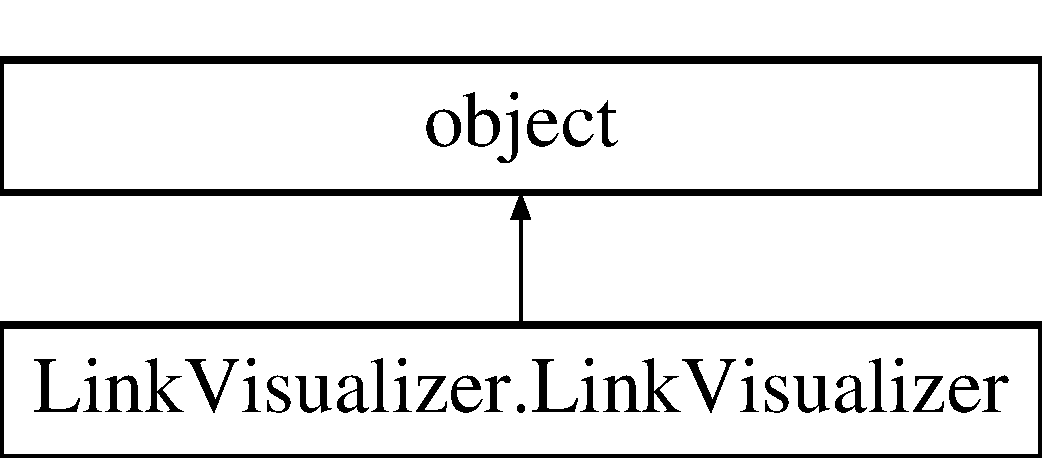
\includegraphics[height=2.000000cm]{class_link_visualizer_1_1_link_visualizer}
\end{center}
\end{figure}
\subsection*{Public Member Functions}
\begin{DoxyCompactItemize}
\item 
def \hyperlink{class_link_visualizer_1_1_link_visualizer_af672a41789fed6cf222a2f531f726944}{\+\_\+\+\_\+init\+\_\+\+\_\+} (self)
\item 
def \hyperlink{class_link_visualizer_1_1_link_visualizer_ac8ef9b117a8c790ecc13174c0d28ab31}{set\+\_\+thickness} (self, th)
\begin{DoxyCompactList}\small\item\em Set the thickness of the link in the Bridge Visualization in pixels; thickness shoudl be in the range 0-\/50.\+0. \end{DoxyCompactList}\item 
def \hyperlink{class_link_visualizer_1_1_link_visualizer_afa1c989f348200429976db98ca91096b}{get\+\_\+thickness} (self)
\begin{DoxyCompactList}\small\item\em Get the thickness of the link in the \hyperlink{namespace_bridges}{Bridges} Visualiation. \end{DoxyCompactList}\item 
def \hyperlink{class_link_visualizer_1_1_link_visualizer_a653ce6a48084bb2b0d506d9ae29d2252}{set\+\_\+weight} (self, wt)
\begin{DoxyCompactList}\small\item\em Set the weight of the link, useful in graph algorithms, for example. \end{DoxyCompactList}\item 
def \hyperlink{class_link_visualizer_1_1_link_visualizer_ac0cedb59b979a4ee18c1f0e149e3dc29}{get\+\_\+weight} (self)
\begin{DoxyCompactList}\small\item\em Get the weight of the link. \end{DoxyCompactList}\item 
def \hyperlink{class_link_visualizer_1_1_link_visualizer_a35d0ecd1bab37fdd82881361999a32c3}{set\+\_\+color}
\begin{DoxyCompactList}\small\item\em Set the color of the link in the \hyperlink{namespace_bridges}{Bridges} Visualization to \char`\"{}a\+Color\char`\"{}. \end{DoxyCompactList}\item 
def \hyperlink{class_link_visualizer_1_1_link_visualizer_a254c9edbc1a75c5f99391ef5f9beb79f}{get\+\_\+color} (self)
\begin{DoxyCompactList}\small\item\em Get the color of the link in the \hyperlink{namespace_bridges}{Bridges} Visualization. \end{DoxyCompactList}\item 
def \hyperlink{class_link_visualizer_1_1_link_visualizer_ac596836b6b514935d6b570168a650ecf}{set\+\_\+opacity} (self, opacity)
\begin{DoxyCompactList}\small\item\em Sets the opacity of the link in the \hyperlink{namespace_bridges}{Bridges} Visualization. \end{DoxyCompactList}\item 
def \hyperlink{class_link_visualizer_1_1_link_visualizer_a62474acb1e264374ddc480831c840437}{get\+\_\+opacity} (self)
\begin{DoxyCompactList}\small\item\em Get the opacity of the link in the \hyperlink{namespace_bridges}{Bridges} Visualization. \end{DoxyCompactList}\item 
def \hyperlink{class_link_visualizer_1_1_link_visualizer_ac335facce0d2d03ecdfa66ddf8505c1b}{get\+\_\+link\+\_\+properties} (self)
\end{DoxyCompactItemize}
\subsection*{Public Attributes}
\begin{DoxyCompactItemize}
\item 
\hyperlink{class_link_visualizer_1_1_link_visualizer_a534ed7a306063db52d7b668542f1ebb5}{color}
\item 
\hyperlink{class_link_visualizer_1_1_link_visualizer_af43b27883cc7b1427ad929b8f9717af9}{thickness}
\item 
\hyperlink{class_link_visualizer_1_1_link_visualizer_ab3663261fc964c75d45b76803384d933}{weight}
\item 
\hyperlink{class_link_visualizer_1_1_link_visualizer_a2f23008a3cfa731f1c2ae70e0d84c86b}{red}
\item 
\hyperlink{class_link_visualizer_1_1_link_visualizer_ab6e44bd36d18e8286fbcaa4f8b557e5d}{green}
\item 
\hyperlink{class_link_visualizer_1_1_link_visualizer_a371f7ab740dc13fdb1cf45b09e09f2cb}{blue}
\end{DoxyCompactItemize}
\subsection*{Static Public Attributes}
\begin{DoxyCompactItemize}
\item 
string \hyperlink{class_link_visualizer_1_1_link_visualizer_a595bb37530287561ffcf304343f7cbde}{Q\+U\+O\+T\+E} = \char`\"{}\textbackslash{}\char`\"{}\char`\"{}
\item 
string \hyperlink{class_link_visualizer_1_1_link_visualizer_ad224a39d19962af54d0726969daa2de2}{C\+O\+M\+M\+A} = \char`\"{},\char`\"{}
\item 
string \hyperlink{class_link_visualizer_1_1_link_visualizer_a179dcb192b99a210729db42add346470}{C\+O\+L\+O\+N} = \char`\"{}\+:\char`\"{}
\item 
string \hyperlink{class_link_visualizer_1_1_link_visualizer_a950cd3c24de95491a53c5cdbd4813a90}{O\+P\+E\+N\+\_\+\+C\+U\+R\+L\+Y} = \char`\"{}\{\char`\"{}
\item 
string \hyperlink{class_link_visualizer_1_1_link_visualizer_a32ff73aa930e9c4a76d26912eb0b6fc9}{C\+L\+O\+S\+E\+\_\+\+C\+U\+R\+L\+Y} = \char`\"{}\}\char`\"{}
\item 
string \hyperlink{class_link_visualizer_1_1_link_visualizer_a0c22a31e997863f6cbdb4507ca5eae4a}{O\+P\+E\+N\+\_\+\+P\+A\+R\+E\+N} = \char`\"{}(\char`\"{}
\item 
string \hyperlink{class_link_visualizer_1_1_link_visualizer_a87bf59ceee60cb2820d9fa5f87d8accb}{C\+L\+O\+S\+E\+\_\+\+P\+A\+R\+E\+N} = \char`\"{})\char`\"{}
\item 
string \hyperlink{class_link_visualizer_1_1_link_visualizer_aba39bf04f99a352408ea57a73fccead8}{O\+P\+E\+N\+\_\+\+B\+O\+X} = \char`\"{}\mbox{[}\char`\"{}
\item 
string \hyperlink{class_link_visualizer_1_1_link_visualizer_a53eecc0f75db3bc4f80fd3043371364f}{C\+L\+O\+S\+E\+\_\+\+B\+O\+X} = \char`\"{}\mbox{]}\char`\"{}
\item 
tuple \hyperlink{class_link_visualizer_1_1_link_visualizer_accc3a152b5d7e227803b8dfd80082ff2}{thickness} = float()
\item 
tuple \hyperlink{class_link_visualizer_1_1_link_visualizer_a2bcaeacc143bd2629d2fc7849b895bde}{weight} = float()
\end{DoxyCompactItemize}


\subsection{Detailed Description}
This class maintains the visual attributes of links that join \hyperlink{namespace_bridges}{Bridges} elements. 

Visual properties include color, thickness, and opacity. Objects of this class are stored as part of the \hyperlink{namespace_element}{Element} class. Generally, a user will manipulate the \hyperlink{class_link_visualizer_1_1_link_visualizer}{Link\+Visualizer} returned from the \hyperlink{namespace_element}{Element}\textquotesingle{}s get\+Link\+Visualizer(\+Element it) method (which it is the \hyperlink{namespace_bridges}{Bridges} element this element is linked to), and then set attributes using its methods. Links are utilized in all types of linked lists, tree and graph structures.

Supported attribute values are as follows\+:

{\bfseries Supported Colors (by name)}\+: 

\char`\"{}red\char`\"{}, \char`\"{}green\char`\"{}, \char`\"{}blue\char`\"{},\char`\"{}yellow\char`\"{},\char`\"{}cyan\char`\"{},\char`\"{}magenta\char`\"{}, \char`\"{}white\char`\"{},, \char`\"{}black\char`\"{}, \char`\"{}orange\char`\"{}, \char`\"{}turquoise\char`\"{}, \char`\"{}maroon\char`\"{}, ~\newline
 \char`\"{}aquamarine\char`\"{}, \char`\"{}azure\char`\"{}, \char`\"{}beige\char`\"{}, \char`\"{}brown\char`\"{}, \char`\"{}tan\char`\"{}, \char`\"{}olive\char`\"{}, \char`\"{}chartreuse\char`\"{}, \char`\"{}khaki\char`\"{}, \char`\"{}bisque\char`\"{}, \char`\"{}coral\char`\"{}, ~\newline
 \char`\"{}pink\char`\"{}, \char`\"{}lavender\char`\"{}, \char`\"{}purple\char`\"{}, \char`\"{}gold\char`\"{} 

{\bfseries  \hyperlink{namespace_color}{Color} by R\+G\+B\+A Specification \+:} Range\+: 0-\/255 for each component 

{\bfseries  Thickness\+: } Range \+: 0.\+0-\/50.\+0

{\bfseries  Opacity\+: } Range (0.\+0-\/1.\+0) 

\begin{DoxyAuthor}{Author}
Mihai Mehedint, Kalpathi Subramanian
\end{DoxyAuthor}
\begin{DoxyDate}{Date}
6/22/16, 1/16/17, 5/17/17
\end{DoxyDate}
\begin{DoxySeeAlso}{See also}
Example Tutorial at ~\newline
 \href{http://bridgesuncc.github.io/Hello_World_Tutorials/SLL.html}{\tt http\+://bridgesuncc.\+github.\+io/\+Hello\+\_\+\+World\+\_\+\+Tutorials/\+S\+L\+L.\+html} 
\end{DoxySeeAlso}


\subsection{Constructor \& Destructor Documentation}
\hypertarget{class_link_visualizer_1_1_link_visualizer_af672a41789fed6cf222a2f531f726944}{}\index{Link\+Visualizer\+::\+Link\+Visualizer@{Link\+Visualizer\+::\+Link\+Visualizer}!\+\_\+\+\_\+init\+\_\+\+\_\+@{\+\_\+\+\_\+init\+\_\+\+\_\+}}
\index{\+\_\+\+\_\+init\+\_\+\+\_\+@{\+\_\+\+\_\+init\+\_\+\+\_\+}!Link\+Visualizer\+::\+Link\+Visualizer@{Link\+Visualizer\+::\+Link\+Visualizer}}
\subsubsection[{\+\_\+\+\_\+init\+\_\+\+\_\+(self)}]{\setlength{\rightskip}{0pt plus 5cm}def Link\+Visualizer.\+Link\+Visualizer.\+\_\+\+\_\+init\+\_\+\+\_\+ (
\begin{DoxyParamCaption}
\item[{}]{self}
\end{DoxyParamCaption}
)}\label{class_link_visualizer_1_1_link_visualizer_af672a41789fed6cf222a2f531f726944}


\subsection{Member Function Documentation}
\hypertarget{class_link_visualizer_1_1_link_visualizer_a254c9edbc1a75c5f99391ef5f9beb79f}{}\index{Link\+Visualizer\+::\+Link\+Visualizer@{Link\+Visualizer\+::\+Link\+Visualizer}!get\+\_\+color@{get\+\_\+color}}
\index{get\+\_\+color@{get\+\_\+color}!Link\+Visualizer\+::\+Link\+Visualizer@{Link\+Visualizer\+::\+Link\+Visualizer}}
\subsubsection[{get\+\_\+color(self)}]{\setlength{\rightskip}{0pt plus 5cm}def Link\+Visualizer.\+Link\+Visualizer.\+get\+\_\+color (
\begin{DoxyParamCaption}
\item[{}]{self}
\end{DoxyParamCaption}
)}\label{class_link_visualizer_1_1_link_visualizer_a254c9edbc1a75c5f99391ef5f9beb79f}


Get the color of the link in the \hyperlink{namespace_bridges}{Bridges} Visualization. 

\begin{DoxyReturn}{Returns}
the \hyperlink{namespace_color}{Color} object representing the color of the link 
\end{DoxyReturn}
\hypertarget{class_link_visualizer_1_1_link_visualizer_ac335facce0d2d03ecdfa66ddf8505c1b}{}\index{Link\+Visualizer\+::\+Link\+Visualizer@{Link\+Visualizer\+::\+Link\+Visualizer}!get\+\_\+link\+\_\+properties@{get\+\_\+link\+\_\+properties}}
\index{get\+\_\+link\+\_\+properties@{get\+\_\+link\+\_\+properties}!Link\+Visualizer\+::\+Link\+Visualizer@{Link\+Visualizer\+::\+Link\+Visualizer}}
\subsubsection[{get\+\_\+link\+\_\+properties(self)}]{\setlength{\rightskip}{0pt plus 5cm}def Link\+Visualizer.\+Link\+Visualizer.\+get\+\_\+link\+\_\+properties (
\begin{DoxyParamCaption}
\item[{}]{self}
\end{DoxyParamCaption}
)}\label{class_link_visualizer_1_1_link_visualizer_ac335facce0d2d03ecdfa66ddf8505c1b}
\hypertarget{class_link_visualizer_1_1_link_visualizer_a62474acb1e264374ddc480831c840437}{}\index{Link\+Visualizer\+::\+Link\+Visualizer@{Link\+Visualizer\+::\+Link\+Visualizer}!get\+\_\+opacity@{get\+\_\+opacity}}
\index{get\+\_\+opacity@{get\+\_\+opacity}!Link\+Visualizer\+::\+Link\+Visualizer@{Link\+Visualizer\+::\+Link\+Visualizer}}
\subsubsection[{get\+\_\+opacity(self)}]{\setlength{\rightskip}{0pt plus 5cm}def Link\+Visualizer.\+Link\+Visualizer.\+get\+\_\+opacity (
\begin{DoxyParamCaption}
\item[{}]{self}
\end{DoxyParamCaption}
)}\label{class_link_visualizer_1_1_link_visualizer_a62474acb1e264374ddc480831c840437}


Get the opacity of the link in the \hyperlink{namespace_bridges}{Bridges} Visualization. 

\begin{DoxyReturn}{Returns}
the opacity value (in the range 0.\+0-\/1.\+0 
\end{DoxyReturn}
\hypertarget{class_link_visualizer_1_1_link_visualizer_afa1c989f348200429976db98ca91096b}{}\index{Link\+Visualizer\+::\+Link\+Visualizer@{Link\+Visualizer\+::\+Link\+Visualizer}!get\+\_\+thickness@{get\+\_\+thickness}}
\index{get\+\_\+thickness@{get\+\_\+thickness}!Link\+Visualizer\+::\+Link\+Visualizer@{Link\+Visualizer\+::\+Link\+Visualizer}}
\subsubsection[{get\+\_\+thickness(self)}]{\setlength{\rightskip}{0pt plus 5cm}def Link\+Visualizer.\+Link\+Visualizer.\+get\+\_\+thickness (
\begin{DoxyParamCaption}
\item[{}]{self}
\end{DoxyParamCaption}
)}\label{class_link_visualizer_1_1_link_visualizer_afa1c989f348200429976db98ca91096b}


Get the thickness of the link in the \hyperlink{namespace_bridges}{Bridges} Visualiation. 

\begin{DoxyReturn}{Returns}
the size in pixels of the \hyperlink{namespace_element}{Element} in the \hyperlink{namespace_bridges}{Bridges} Visualization 
\end{DoxyReturn}
\hypertarget{class_link_visualizer_1_1_link_visualizer_ac0cedb59b979a4ee18c1f0e149e3dc29}{}\index{Link\+Visualizer\+::\+Link\+Visualizer@{Link\+Visualizer\+::\+Link\+Visualizer}!get\+\_\+weight@{get\+\_\+weight}}
\index{get\+\_\+weight@{get\+\_\+weight}!Link\+Visualizer\+::\+Link\+Visualizer@{Link\+Visualizer\+::\+Link\+Visualizer}}
\subsubsection[{get\+\_\+weight(self)}]{\setlength{\rightskip}{0pt plus 5cm}def Link\+Visualizer.\+Link\+Visualizer.\+get\+\_\+weight (
\begin{DoxyParamCaption}
\item[{}]{self}
\end{DoxyParamCaption}
)}\label{class_link_visualizer_1_1_link_visualizer_ac0cedb59b979a4ee18c1f0e149e3dc29}


Get the weight of the link. 

\begin{DoxyReturn}{Returns}
the stored edge weight 
\end{DoxyReturn}
\hypertarget{class_link_visualizer_1_1_link_visualizer_a35d0ecd1bab37fdd82881361999a32c3}{}\index{Link\+Visualizer\+::\+Link\+Visualizer@{Link\+Visualizer\+::\+Link\+Visualizer}!set\+\_\+color@{set\+\_\+color}}
\index{set\+\_\+color@{set\+\_\+color}!Link\+Visualizer\+::\+Link\+Visualizer@{Link\+Visualizer\+::\+Link\+Visualizer}}
\subsubsection[{set\+\_\+color}]{\setlength{\rightskip}{0pt plus 5cm}def Link\+Visualizer.\+Link\+Visualizer.\+set\+\_\+color (
\begin{DoxyParamCaption}
\item[{}]{self, }
\item[{}]{col\+\_\+name = {\ttfamily None}, }
\item[{}]{r = {\ttfamily None}, }
\item[{}]{g = {\ttfamily None}, }
\item[{}]{b = {\ttfamily None}, }
\item[{}]{a = {\ttfamily None}}
\end{DoxyParamCaption}
)}\label{class_link_visualizer_1_1_link_visualizer_a35d0ecd1bab37fdd82881361999a32c3}


Set the color of the link in the \hyperlink{namespace_bridges}{Bridges} Visualization to \char`\"{}a\+Color\char`\"{}. 


\begin{DoxyParams}{Parameters}
{\em col\+\_\+name} & the string reprsenting the color of the \hyperlink{namespace_element}{Element} in the \hyperlink{namespace_bridges}{Bridges} Visualization; supported named colors are \char`\"{}red\char`\"{}, \char`\"{}green\char`\"{}, \char`\"{}blue\char`\"{}, \char`\"{}yellow\char`\"{}, \char`\"{}cyan\char`\"{}, \char`\"{}magenta\char`\"{}, \char`\"{}white\char`\"{}, \char`\"{}black\char`\"{}, \char`\"{}orange\char`\"{}, \char`\"{}turquoise\char`\"{}, \char`\"{}maroon\char`\"{}, \char`\"{}aquamarine\char`\"{}, \char`\"{}azure\char`\"{}, \char`\"{}beige\char`\"{}, \char`\"{}brown\char`\"{}, \char`\"{}tan\char`\"{}, \char`\"{}olive\char`\"{}, \char`\"{}chartreuse\char`\"{}, \char`\"{}khaki\char`\"{}, \char`\"{}bisque\char`\"{}, \char`\"{}coral\char`\"{}, \char`\"{}pink\char`\"{}, \char`\"{}lavender\char`\"{}, \char`\"{}purple\char`\"{}, \char`\"{}gold\char`\"{} \\
\hline
\end{DoxyParams}
\hypertarget{class_link_visualizer_1_1_link_visualizer_ac596836b6b514935d6b570168a650ecf}{}\index{Link\+Visualizer\+::\+Link\+Visualizer@{Link\+Visualizer\+::\+Link\+Visualizer}!set\+\_\+opacity@{set\+\_\+opacity}}
\index{set\+\_\+opacity@{set\+\_\+opacity}!Link\+Visualizer\+::\+Link\+Visualizer@{Link\+Visualizer\+::\+Link\+Visualizer}}
\subsubsection[{set\+\_\+opacity(self, opacity)}]{\setlength{\rightskip}{0pt plus 5cm}def Link\+Visualizer.\+Link\+Visualizer.\+set\+\_\+opacity (
\begin{DoxyParamCaption}
\item[{}]{self, }
\item[{}]{opacity}
\end{DoxyParamCaption}
)}\label{class_link_visualizer_1_1_link_visualizer_ac596836b6b514935d6b570168a650ecf}


Sets the opacity of the link in the \hyperlink{namespace_bridges}{Bridges} Visualization. 


\begin{DoxyParams}{Parameters}
{\em opacity} & a float between 0 and 1 representing how transparent the node should be on the \hyperlink{namespace_bridges}{Bridges} Visualization. 0 for invisible, 1 for fully visible, a decimal between 0 and 1 for varying transparency. \\
\hline
\end{DoxyParams}
\hypertarget{class_link_visualizer_1_1_link_visualizer_ac8ef9b117a8c790ecc13174c0d28ab31}{}\index{Link\+Visualizer\+::\+Link\+Visualizer@{Link\+Visualizer\+::\+Link\+Visualizer}!set\+\_\+thickness@{set\+\_\+thickness}}
\index{set\+\_\+thickness@{set\+\_\+thickness}!Link\+Visualizer\+::\+Link\+Visualizer@{Link\+Visualizer\+::\+Link\+Visualizer}}
\subsubsection[{set\+\_\+thickness(self, th)}]{\setlength{\rightskip}{0pt plus 5cm}def Link\+Visualizer.\+Link\+Visualizer.\+set\+\_\+thickness (
\begin{DoxyParamCaption}
\item[{}]{self, }
\item[{}]{th}
\end{DoxyParamCaption}
)}\label{class_link_visualizer_1_1_link_visualizer_ac8ef9b117a8c790ecc13174c0d28ab31}


Set the thickness of the link in the Bridge Visualization in pixels; thickness shoudl be in the range 0-\/50.\+0. 


\begin{DoxyParams}{Parameters}
{\em thickness} & \\
\hline
\end{DoxyParams}
\hypertarget{class_link_visualizer_1_1_link_visualizer_a653ce6a48084bb2b0d506d9ae29d2252}{}\index{Link\+Visualizer\+::\+Link\+Visualizer@{Link\+Visualizer\+::\+Link\+Visualizer}!set\+\_\+weight@{set\+\_\+weight}}
\index{set\+\_\+weight@{set\+\_\+weight}!Link\+Visualizer\+::\+Link\+Visualizer@{Link\+Visualizer\+::\+Link\+Visualizer}}
\subsubsection[{set\+\_\+weight(self, wt)}]{\setlength{\rightskip}{0pt plus 5cm}def Link\+Visualizer.\+Link\+Visualizer.\+set\+\_\+weight (
\begin{DoxyParamCaption}
\item[{}]{self, }
\item[{}]{wt}
\end{DoxyParamCaption}
)}\label{class_link_visualizer_1_1_link_visualizer_a653ce6a48084bb2b0d506d9ae29d2252}


Set the weight of the link, useful in graph algorithms, for example. 

weight value is user defined, and determined by the input graph specification.


\begin{DoxyParams}{Parameters}
{\em weight} & \\
\hline
\end{DoxyParams}


\subsection{Member Data Documentation}
\hypertarget{class_link_visualizer_1_1_link_visualizer_a371f7ab740dc13fdb1cf45b09e09f2cb}{}\index{Link\+Visualizer\+::\+Link\+Visualizer@{Link\+Visualizer\+::\+Link\+Visualizer}!blue@{blue}}
\index{blue@{blue}!Link\+Visualizer\+::\+Link\+Visualizer@{Link\+Visualizer\+::\+Link\+Visualizer}}
\subsubsection[{blue}]{\setlength{\rightskip}{0pt plus 5cm}Link\+Visualizer.\+Link\+Visualizer.\+blue}\label{class_link_visualizer_1_1_link_visualizer_a371f7ab740dc13fdb1cf45b09e09f2cb}
\hypertarget{class_link_visualizer_1_1_link_visualizer_a53eecc0f75db3bc4f80fd3043371364f}{}\index{Link\+Visualizer\+::\+Link\+Visualizer@{Link\+Visualizer\+::\+Link\+Visualizer}!C\+L\+O\+S\+E\+\_\+\+B\+O\+X@{C\+L\+O\+S\+E\+\_\+\+B\+O\+X}}
\index{C\+L\+O\+S\+E\+\_\+\+B\+O\+X@{C\+L\+O\+S\+E\+\_\+\+B\+O\+X}!Link\+Visualizer\+::\+Link\+Visualizer@{Link\+Visualizer\+::\+Link\+Visualizer}}
\subsubsection[{C\+L\+O\+S\+E\+\_\+\+B\+O\+X}]{\setlength{\rightskip}{0pt plus 5cm}string Link\+Visualizer.\+Link\+Visualizer.\+C\+L\+O\+S\+E\+\_\+\+B\+O\+X = \char`\"{}\mbox{]}\char`\"{}\hspace{0.3cm}{\ttfamily [static]}}\label{class_link_visualizer_1_1_link_visualizer_a53eecc0f75db3bc4f80fd3043371364f}
\hypertarget{class_link_visualizer_1_1_link_visualizer_a32ff73aa930e9c4a76d26912eb0b6fc9}{}\index{Link\+Visualizer\+::\+Link\+Visualizer@{Link\+Visualizer\+::\+Link\+Visualizer}!C\+L\+O\+S\+E\+\_\+\+C\+U\+R\+L\+Y@{C\+L\+O\+S\+E\+\_\+\+C\+U\+R\+L\+Y}}
\index{C\+L\+O\+S\+E\+\_\+\+C\+U\+R\+L\+Y@{C\+L\+O\+S\+E\+\_\+\+C\+U\+R\+L\+Y}!Link\+Visualizer\+::\+Link\+Visualizer@{Link\+Visualizer\+::\+Link\+Visualizer}}
\subsubsection[{C\+L\+O\+S\+E\+\_\+\+C\+U\+R\+L\+Y}]{\setlength{\rightskip}{0pt plus 5cm}string Link\+Visualizer.\+Link\+Visualizer.\+C\+L\+O\+S\+E\+\_\+\+C\+U\+R\+L\+Y = \char`\"{}\}\char`\"{}\hspace{0.3cm}{\ttfamily [static]}}\label{class_link_visualizer_1_1_link_visualizer_a32ff73aa930e9c4a76d26912eb0b6fc9}
\hypertarget{class_link_visualizer_1_1_link_visualizer_a87bf59ceee60cb2820d9fa5f87d8accb}{}\index{Link\+Visualizer\+::\+Link\+Visualizer@{Link\+Visualizer\+::\+Link\+Visualizer}!C\+L\+O\+S\+E\+\_\+\+P\+A\+R\+E\+N@{C\+L\+O\+S\+E\+\_\+\+P\+A\+R\+E\+N}}
\index{C\+L\+O\+S\+E\+\_\+\+P\+A\+R\+E\+N@{C\+L\+O\+S\+E\+\_\+\+P\+A\+R\+E\+N}!Link\+Visualizer\+::\+Link\+Visualizer@{Link\+Visualizer\+::\+Link\+Visualizer}}
\subsubsection[{C\+L\+O\+S\+E\+\_\+\+P\+A\+R\+E\+N}]{\setlength{\rightskip}{0pt plus 5cm}string Link\+Visualizer.\+Link\+Visualizer.\+C\+L\+O\+S\+E\+\_\+\+P\+A\+R\+E\+N = \char`\"{})\char`\"{}\hspace{0.3cm}{\ttfamily [static]}}\label{class_link_visualizer_1_1_link_visualizer_a87bf59ceee60cb2820d9fa5f87d8accb}
\hypertarget{class_link_visualizer_1_1_link_visualizer_a179dcb192b99a210729db42add346470}{}\index{Link\+Visualizer\+::\+Link\+Visualizer@{Link\+Visualizer\+::\+Link\+Visualizer}!C\+O\+L\+O\+N@{C\+O\+L\+O\+N}}
\index{C\+O\+L\+O\+N@{C\+O\+L\+O\+N}!Link\+Visualizer\+::\+Link\+Visualizer@{Link\+Visualizer\+::\+Link\+Visualizer}}
\subsubsection[{C\+O\+L\+O\+N}]{\setlength{\rightskip}{0pt plus 5cm}string Link\+Visualizer.\+Link\+Visualizer.\+C\+O\+L\+O\+N = \char`\"{}\+:\char`\"{}\hspace{0.3cm}{\ttfamily [static]}}\label{class_link_visualizer_1_1_link_visualizer_a179dcb192b99a210729db42add346470}
\hypertarget{class_link_visualizer_1_1_link_visualizer_a534ed7a306063db52d7b668542f1ebb5}{}\index{Link\+Visualizer\+::\+Link\+Visualizer@{Link\+Visualizer\+::\+Link\+Visualizer}!color@{color}}
\index{color@{color}!Link\+Visualizer\+::\+Link\+Visualizer@{Link\+Visualizer\+::\+Link\+Visualizer}}
\subsubsection[{color}]{\setlength{\rightskip}{0pt plus 5cm}Link\+Visualizer.\+Link\+Visualizer.\+color}\label{class_link_visualizer_1_1_link_visualizer_a534ed7a306063db52d7b668542f1ebb5}
\hypertarget{class_link_visualizer_1_1_link_visualizer_ad224a39d19962af54d0726969daa2de2}{}\index{Link\+Visualizer\+::\+Link\+Visualizer@{Link\+Visualizer\+::\+Link\+Visualizer}!C\+O\+M\+M\+A@{C\+O\+M\+M\+A}}
\index{C\+O\+M\+M\+A@{C\+O\+M\+M\+A}!Link\+Visualizer\+::\+Link\+Visualizer@{Link\+Visualizer\+::\+Link\+Visualizer}}
\subsubsection[{C\+O\+M\+M\+A}]{\setlength{\rightskip}{0pt plus 5cm}string Link\+Visualizer.\+Link\+Visualizer.\+C\+O\+M\+M\+A = \char`\"{},\char`\"{}\hspace{0.3cm}{\ttfamily [static]}}\label{class_link_visualizer_1_1_link_visualizer_ad224a39d19962af54d0726969daa2de2}
\hypertarget{class_link_visualizer_1_1_link_visualizer_ab6e44bd36d18e8286fbcaa4f8b557e5d}{}\index{Link\+Visualizer\+::\+Link\+Visualizer@{Link\+Visualizer\+::\+Link\+Visualizer}!green@{green}}
\index{green@{green}!Link\+Visualizer\+::\+Link\+Visualizer@{Link\+Visualizer\+::\+Link\+Visualizer}}
\subsubsection[{green}]{\setlength{\rightskip}{0pt plus 5cm}Link\+Visualizer.\+Link\+Visualizer.\+green}\label{class_link_visualizer_1_1_link_visualizer_ab6e44bd36d18e8286fbcaa4f8b557e5d}
\hypertarget{class_link_visualizer_1_1_link_visualizer_aba39bf04f99a352408ea57a73fccead8}{}\index{Link\+Visualizer\+::\+Link\+Visualizer@{Link\+Visualizer\+::\+Link\+Visualizer}!O\+P\+E\+N\+\_\+\+B\+O\+X@{O\+P\+E\+N\+\_\+\+B\+O\+X}}
\index{O\+P\+E\+N\+\_\+\+B\+O\+X@{O\+P\+E\+N\+\_\+\+B\+O\+X}!Link\+Visualizer\+::\+Link\+Visualizer@{Link\+Visualizer\+::\+Link\+Visualizer}}
\subsubsection[{O\+P\+E\+N\+\_\+\+B\+O\+X}]{\setlength{\rightskip}{0pt plus 5cm}string Link\+Visualizer.\+Link\+Visualizer.\+O\+P\+E\+N\+\_\+\+B\+O\+X = \char`\"{}\mbox{[}\char`\"{}\hspace{0.3cm}{\ttfamily [static]}}\label{class_link_visualizer_1_1_link_visualizer_aba39bf04f99a352408ea57a73fccead8}
\hypertarget{class_link_visualizer_1_1_link_visualizer_a950cd3c24de95491a53c5cdbd4813a90}{}\index{Link\+Visualizer\+::\+Link\+Visualizer@{Link\+Visualizer\+::\+Link\+Visualizer}!O\+P\+E\+N\+\_\+\+C\+U\+R\+L\+Y@{O\+P\+E\+N\+\_\+\+C\+U\+R\+L\+Y}}
\index{O\+P\+E\+N\+\_\+\+C\+U\+R\+L\+Y@{O\+P\+E\+N\+\_\+\+C\+U\+R\+L\+Y}!Link\+Visualizer\+::\+Link\+Visualizer@{Link\+Visualizer\+::\+Link\+Visualizer}}
\subsubsection[{O\+P\+E\+N\+\_\+\+C\+U\+R\+L\+Y}]{\setlength{\rightskip}{0pt plus 5cm}string Link\+Visualizer.\+Link\+Visualizer.\+O\+P\+E\+N\+\_\+\+C\+U\+R\+L\+Y = \char`\"{}\{\char`\"{}\hspace{0.3cm}{\ttfamily [static]}}\label{class_link_visualizer_1_1_link_visualizer_a950cd3c24de95491a53c5cdbd4813a90}
\hypertarget{class_link_visualizer_1_1_link_visualizer_a0c22a31e997863f6cbdb4507ca5eae4a}{}\index{Link\+Visualizer\+::\+Link\+Visualizer@{Link\+Visualizer\+::\+Link\+Visualizer}!O\+P\+E\+N\+\_\+\+P\+A\+R\+E\+N@{O\+P\+E\+N\+\_\+\+P\+A\+R\+E\+N}}
\index{O\+P\+E\+N\+\_\+\+P\+A\+R\+E\+N@{O\+P\+E\+N\+\_\+\+P\+A\+R\+E\+N}!Link\+Visualizer\+::\+Link\+Visualizer@{Link\+Visualizer\+::\+Link\+Visualizer}}
\subsubsection[{O\+P\+E\+N\+\_\+\+P\+A\+R\+E\+N}]{\setlength{\rightskip}{0pt plus 5cm}string Link\+Visualizer.\+Link\+Visualizer.\+O\+P\+E\+N\+\_\+\+P\+A\+R\+E\+N = \char`\"{}(\char`\"{}\hspace{0.3cm}{\ttfamily [static]}}\label{class_link_visualizer_1_1_link_visualizer_a0c22a31e997863f6cbdb4507ca5eae4a}
\hypertarget{class_link_visualizer_1_1_link_visualizer_a595bb37530287561ffcf304343f7cbde}{}\index{Link\+Visualizer\+::\+Link\+Visualizer@{Link\+Visualizer\+::\+Link\+Visualizer}!Q\+U\+O\+T\+E@{Q\+U\+O\+T\+E}}
\index{Q\+U\+O\+T\+E@{Q\+U\+O\+T\+E}!Link\+Visualizer\+::\+Link\+Visualizer@{Link\+Visualizer\+::\+Link\+Visualizer}}
\subsubsection[{Q\+U\+O\+T\+E}]{\setlength{\rightskip}{0pt plus 5cm}string Link\+Visualizer.\+Link\+Visualizer.\+Q\+U\+O\+T\+E = \char`\"{}\textbackslash{}\char`\"{}\char`\"{}\hspace{0.3cm}{\ttfamily [static]}}\label{class_link_visualizer_1_1_link_visualizer_a595bb37530287561ffcf304343f7cbde}
\hypertarget{class_link_visualizer_1_1_link_visualizer_a2f23008a3cfa731f1c2ae70e0d84c86b}{}\index{Link\+Visualizer\+::\+Link\+Visualizer@{Link\+Visualizer\+::\+Link\+Visualizer}!red@{red}}
\index{red@{red}!Link\+Visualizer\+::\+Link\+Visualizer@{Link\+Visualizer\+::\+Link\+Visualizer}}
\subsubsection[{red}]{\setlength{\rightskip}{0pt plus 5cm}Link\+Visualizer.\+Link\+Visualizer.\+red}\label{class_link_visualizer_1_1_link_visualizer_a2f23008a3cfa731f1c2ae70e0d84c86b}
\hypertarget{class_link_visualizer_1_1_link_visualizer_accc3a152b5d7e227803b8dfd80082ff2}{}\index{Link\+Visualizer\+::\+Link\+Visualizer@{Link\+Visualizer\+::\+Link\+Visualizer}!thickness@{thickness}}
\index{thickness@{thickness}!Link\+Visualizer\+::\+Link\+Visualizer@{Link\+Visualizer\+::\+Link\+Visualizer}}
\subsubsection[{thickness}]{\setlength{\rightskip}{0pt plus 5cm}tuple Link\+Visualizer.\+Link\+Visualizer.\+thickness = float()\hspace{0.3cm}{\ttfamily [static]}}\label{class_link_visualizer_1_1_link_visualizer_accc3a152b5d7e227803b8dfd80082ff2}
\hypertarget{class_link_visualizer_1_1_link_visualizer_af43b27883cc7b1427ad929b8f9717af9}{}\index{Link\+Visualizer\+::\+Link\+Visualizer@{Link\+Visualizer\+::\+Link\+Visualizer}!thickness@{thickness}}
\index{thickness@{thickness}!Link\+Visualizer\+::\+Link\+Visualizer@{Link\+Visualizer\+::\+Link\+Visualizer}}
\subsubsection[{thickness}]{\setlength{\rightskip}{0pt plus 5cm}Link\+Visualizer.\+Link\+Visualizer.\+thickness}\label{class_link_visualizer_1_1_link_visualizer_af43b27883cc7b1427ad929b8f9717af9}
\hypertarget{class_link_visualizer_1_1_link_visualizer_a2bcaeacc143bd2629d2fc7849b895bde}{}\index{Link\+Visualizer\+::\+Link\+Visualizer@{Link\+Visualizer\+::\+Link\+Visualizer}!weight@{weight}}
\index{weight@{weight}!Link\+Visualizer\+::\+Link\+Visualizer@{Link\+Visualizer\+::\+Link\+Visualizer}}
\subsubsection[{weight}]{\setlength{\rightskip}{0pt plus 5cm}tuple Link\+Visualizer.\+Link\+Visualizer.\+weight = float()\hspace{0.3cm}{\ttfamily [static]}}\label{class_link_visualizer_1_1_link_visualizer_a2bcaeacc143bd2629d2fc7849b895bde}
\hypertarget{class_link_visualizer_1_1_link_visualizer_ab3663261fc964c75d45b76803384d933}{}\index{Link\+Visualizer\+::\+Link\+Visualizer@{Link\+Visualizer\+::\+Link\+Visualizer}!weight@{weight}}
\index{weight@{weight}!Link\+Visualizer\+::\+Link\+Visualizer@{Link\+Visualizer\+::\+Link\+Visualizer}}
\subsubsection[{weight}]{\setlength{\rightskip}{0pt plus 5cm}Link\+Visualizer.\+Link\+Visualizer.\+weight}\label{class_link_visualizer_1_1_link_visualizer_ab3663261fc964c75d45b76803384d933}


The documentation for this class was generated from the following file\+:\begin{DoxyCompactItemize}
\item 
/\+Users/krs/gr/bridges/bridges17/python/src/\hyperlink{_link_visualizer_8py}{Link\+Visualizer.\+py}\end{DoxyCompactItemize}

\hypertarget{class_m_lelement_1_1_m_lelement}{}\section{M\+Lelement.\+M\+Lelement Class Reference}
\label{class_m_lelement_1_1_m_lelement}\index{M\+Lelement.\+M\+Lelement@{M\+Lelement.\+M\+Lelement}}


This class can be used to instantiate Multi-\/list Elements.  


Inheritance diagram for M\+Lelement.\+M\+Lelement\+:\begin{figure}[H]
\begin{center}
\leavevmode
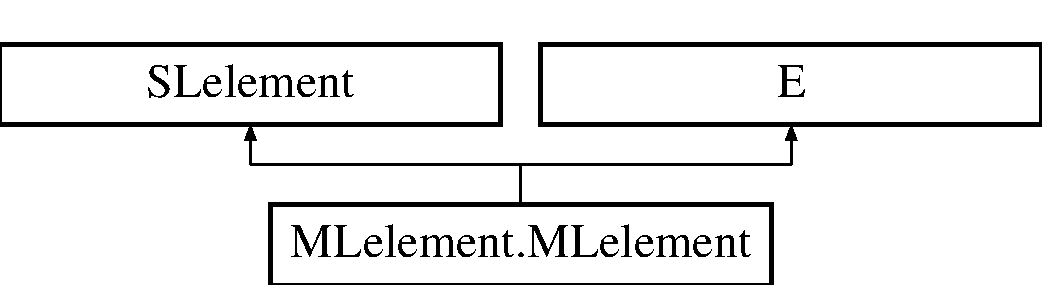
\includegraphics[height=4.000000cm]{class_m_lelement_1_1_m_lelement}
\end{center}
\end{figure}
\subsection*{Public Member Functions}
\begin{DoxyCompactItemize}
\item 
def \hyperlink{class_m_lelement_1_1_m_lelement_a4d3cb3ab25392cec8cdb9dbe5355a13a}{\+\_\+\+\_\+init\+\_\+\+\_\+}
\begin{DoxyCompactList}\small\item\em This constructor creates an \hyperlink{namespace_s_lelement}{S\+Lelement} object and sets the next pointer to null. \end{DoxyCompactList}\item 
def \hyperlink{class_m_lelement_1_1_m_lelement_a31c67e22d2ab911d2fd4dd4f9946f446}{set\+\_\+sub\+\_\+list} (self, sl)
\begin{DoxyCompactList}\small\item\em Sets the start of a new sublist. \end{DoxyCompactList}\item 
def \hyperlink{class_m_lelement_1_1_m_lelement_a9bb9492125f9286490490dba9f8a21c8}{get\+\_\+sub\+\_\+list} (self)
\item 
def \hyperlink{class_m_lelement_1_1_m_lelement_a791214b54150e22d4aa0a2c06c645ca9}{get\+\_\+data\+\_\+structure\+\_\+type} (self)
\item 
def \hyperlink{class_m_lelement_1_1_m_lelement_a2eb5ffdbd27405b5198f517d1e0dd8d9}{get\+\_\+next} (self)
\item 
def \hyperlink{class_m_lelement_1_1_m_lelement_a2eb7bfecd1603a4b252f26b7151a9b16}{set\+\_\+tag} (self, t)
\item 
def \hyperlink{class_m_lelement_1_1_m_lelement_a51e0d540f1bac98a09310d7d3164a4f8}{get\+\_\+tag} (self)
\item 
def \hyperlink{class_m_lelement_1_1_m_lelement_ab2c638b975a778dfb7af3e9a34b21d2a}{get\+\_\+data\+\_\+structure\+\_\+representation} (self)
\item 
def \hyperlink{class_m_lelement_1_1_m_lelement_ae50af379b2c5e8f899c618c96d58831b}{get\+\_\+list\+\_\+elements} (self, nodes)
\item 
def \hyperlink{class_m_lelement_1_1_m_lelement_a92d1ede5bcca05bd4140e4a2d3623d2c}{get\+\_\+list\+\_\+elements\+\_\+\+R} (self, list, nodes)
\end{DoxyCompactItemize}
\subsection*{Static Public Attributes}
\begin{DoxyCompactItemize}
\item 
\hyperlink{class_m_lelement_1_1_m_lelement_a03b2df3aa731f864b628ff60dda11a30}{sub\+\_\+list} = None
\item 
\hyperlink{class_m_lelement_1_1_m_lelement_ae7e3455395f34a27e1a7e8fa26adce50}{tag} = False
\end{DoxyCompactItemize}
\subsection*{Additional Inherited Members}


\subsection{Detailed Description}
This class can be used to instantiate Multi-\/list Elements. 

This class extends \hyperlink{namespace_s_lelement}{S\+Lelement} (singly linked list element) to build multi-\/lists; Multilist elements contain a tag that indicates if the element is a sublist or not; If the element points to a sublist, then the sublist field is the beginning of this sublist. If not, the data field contains the user specified data item and list continues (get\+Next()/set\+Next()). As in singly linked elements, the next pointer points to the following list element of the list or sublist.

Multi-\/list elements contain a visualizer (\hyperlink{namespace_element_visualizer}{Element\+Visualizer}) object for setting visual attributes (color, shape, opacity, size), necessary for displaying them in a web browser.

Elements also have a \hyperlink{namespace_link_visualizer}{Link\+Visualizer} object, that is used when they are linked to another element, appropriate for setting link attributes, for instance, between the current element and its next element. In this case, the link in question is that which connects the element to the following elements; a similar logic follows for sublists.

\begin{DoxyAuthor}{Author}
, Kalpathi Subramanian
\end{DoxyAuthor}
\begin{DoxyDate}{Date}
5/24/17
\end{DoxyDate}

\begin{DoxyParams}{Parameters}
{\em $<$\+E$>$} & The generic parameter object that is part of this element, representing either application specific data, or a pointer to a sublist.\\
\hline
\end{DoxyParams}
\begin{DoxySeeAlso}{See also}
Example Tutorial at ~\newline
 ?? 
\end{DoxySeeAlso}


\subsection{Constructor \& Destructor Documentation}
\hypertarget{class_m_lelement_1_1_m_lelement_a4d3cb3ab25392cec8cdb9dbe5355a13a}{}\index{M\+Lelement\+::\+M\+Lelement@{M\+Lelement\+::\+M\+Lelement}!\+\_\+\+\_\+init\+\_\+\+\_\+@{\+\_\+\+\_\+init\+\_\+\+\_\+}}
\index{\+\_\+\+\_\+init\+\_\+\+\_\+@{\+\_\+\+\_\+init\+\_\+\+\_\+}!M\+Lelement\+::\+M\+Lelement@{M\+Lelement\+::\+M\+Lelement}}
\subsubsection[{\+\_\+\+\_\+init\+\_\+\+\_\+}]{\setlength{\rightskip}{0pt plus 5cm}def M\+Lelement.\+M\+Lelement.\+\_\+\+\_\+init\+\_\+\+\_\+ (
\begin{DoxyParamCaption}
\item[{}]{self, }
\item[{}]{label = {\ttfamily None}, }
\item[{}]{e = {\ttfamily None}, }
\item[{}]{next = {\ttfamily None}, }
\item[{}]{sublist = {\ttfamily None}}
\end{DoxyParamCaption}
)}\label{class_m_lelement_1_1_m_lelement_a4d3cb3ab25392cec8cdb9dbe5355a13a}


This constructor creates an \hyperlink{namespace_s_lelement}{S\+Lelement} object and sets the next pointer to null. 



\subsection{Member Function Documentation}
\hypertarget{class_m_lelement_1_1_m_lelement_ab2c638b975a778dfb7af3e9a34b21d2a}{}\index{M\+Lelement\+::\+M\+Lelement@{M\+Lelement\+::\+M\+Lelement}!get\+\_\+data\+\_\+structure\+\_\+representation@{get\+\_\+data\+\_\+structure\+\_\+representation}}
\index{get\+\_\+data\+\_\+structure\+\_\+representation@{get\+\_\+data\+\_\+structure\+\_\+representation}!M\+Lelement\+::\+M\+Lelement@{M\+Lelement\+::\+M\+Lelement}}
\subsubsection[{get\+\_\+data\+\_\+structure\+\_\+representation(self)}]{\setlength{\rightskip}{0pt plus 5cm}def M\+Lelement.\+M\+Lelement.\+get\+\_\+data\+\_\+structure\+\_\+representation (
\begin{DoxyParamCaption}
\item[{}]{self}
\end{DoxyParamCaption}
)}\label{class_m_lelement_1_1_m_lelement_ab2c638b975a778dfb7af3e9a34b21d2a}
\hypertarget{class_m_lelement_1_1_m_lelement_a791214b54150e22d4aa0a2c06c645ca9}{}\index{M\+Lelement\+::\+M\+Lelement@{M\+Lelement\+::\+M\+Lelement}!get\+\_\+data\+\_\+structure\+\_\+type@{get\+\_\+data\+\_\+structure\+\_\+type}}
\index{get\+\_\+data\+\_\+structure\+\_\+type@{get\+\_\+data\+\_\+structure\+\_\+type}!M\+Lelement\+::\+M\+Lelement@{M\+Lelement\+::\+M\+Lelement}}
\subsubsection[{get\+\_\+data\+\_\+structure\+\_\+type(self)}]{\setlength{\rightskip}{0pt plus 5cm}def M\+Lelement.\+M\+Lelement.\+get\+\_\+data\+\_\+structure\+\_\+type (
\begin{DoxyParamCaption}
\item[{}]{self}
\end{DoxyParamCaption}
)}\label{class_m_lelement_1_1_m_lelement_a791214b54150e22d4aa0a2c06c645ca9}
\hypertarget{class_m_lelement_1_1_m_lelement_ae50af379b2c5e8f899c618c96d58831b}{}\index{M\+Lelement\+::\+M\+Lelement@{M\+Lelement\+::\+M\+Lelement}!get\+\_\+list\+\_\+elements@{get\+\_\+list\+\_\+elements}}
\index{get\+\_\+list\+\_\+elements@{get\+\_\+list\+\_\+elements}!M\+Lelement\+::\+M\+Lelement@{M\+Lelement\+::\+M\+Lelement}}
\subsubsection[{get\+\_\+list\+\_\+elements(self, nodes)}]{\setlength{\rightskip}{0pt plus 5cm}def M\+Lelement.\+M\+Lelement.\+get\+\_\+list\+\_\+elements (
\begin{DoxyParamCaption}
\item[{}]{self, }
\item[{}]{nodes}
\end{DoxyParamCaption}
)}\label{class_m_lelement_1_1_m_lelement_ae50af379b2c5e8f899c618c96d58831b}
\hypertarget{class_m_lelement_1_1_m_lelement_a92d1ede5bcca05bd4140e4a2d3623d2c}{}\index{M\+Lelement\+::\+M\+Lelement@{M\+Lelement\+::\+M\+Lelement}!get\+\_\+list\+\_\+elements\+\_\+\+R@{get\+\_\+list\+\_\+elements\+\_\+\+R}}
\index{get\+\_\+list\+\_\+elements\+\_\+\+R@{get\+\_\+list\+\_\+elements\+\_\+\+R}!M\+Lelement\+::\+M\+Lelement@{M\+Lelement\+::\+M\+Lelement}}
\subsubsection[{get\+\_\+list\+\_\+elements\+\_\+\+R(self, list, nodes)}]{\setlength{\rightskip}{0pt plus 5cm}def M\+Lelement.\+M\+Lelement.\+get\+\_\+list\+\_\+elements\+\_\+\+R (
\begin{DoxyParamCaption}
\item[{}]{self, }
\item[{}]{list, }
\item[{}]{nodes}
\end{DoxyParamCaption}
)}\label{class_m_lelement_1_1_m_lelement_a92d1ede5bcca05bd4140e4a2d3623d2c}
\hypertarget{class_m_lelement_1_1_m_lelement_a2eb5ffdbd27405b5198f517d1e0dd8d9}{}\index{M\+Lelement\+::\+M\+Lelement@{M\+Lelement\+::\+M\+Lelement}!get\+\_\+next@{get\+\_\+next}}
\index{get\+\_\+next@{get\+\_\+next}!M\+Lelement\+::\+M\+Lelement@{M\+Lelement\+::\+M\+Lelement}}
\subsubsection[{get\+\_\+next(self)}]{\setlength{\rightskip}{0pt plus 5cm}def M\+Lelement.\+M\+Lelement.\+get\+\_\+next (
\begin{DoxyParamCaption}
\item[{}]{self}
\end{DoxyParamCaption}
)}\label{class_m_lelement_1_1_m_lelement_a2eb5ffdbd27405b5198f517d1e0dd8d9}
\hypertarget{class_m_lelement_1_1_m_lelement_a9bb9492125f9286490490dba9f8a21c8}{}\index{M\+Lelement\+::\+M\+Lelement@{M\+Lelement\+::\+M\+Lelement}!get\+\_\+sub\+\_\+list@{get\+\_\+sub\+\_\+list}}
\index{get\+\_\+sub\+\_\+list@{get\+\_\+sub\+\_\+list}!M\+Lelement\+::\+M\+Lelement@{M\+Lelement\+::\+M\+Lelement}}
\subsubsection[{get\+\_\+sub\+\_\+list(self)}]{\setlength{\rightskip}{0pt plus 5cm}def M\+Lelement.\+M\+Lelement.\+get\+\_\+sub\+\_\+list (
\begin{DoxyParamCaption}
\item[{}]{self}
\end{DoxyParamCaption}
)}\label{class_m_lelement_1_1_m_lelement_a9bb9492125f9286490490dba9f8a21c8}
\hypertarget{class_m_lelement_1_1_m_lelement_a51e0d540f1bac98a09310d7d3164a4f8}{}\index{M\+Lelement\+::\+M\+Lelement@{M\+Lelement\+::\+M\+Lelement}!get\+\_\+tag@{get\+\_\+tag}}
\index{get\+\_\+tag@{get\+\_\+tag}!M\+Lelement\+::\+M\+Lelement@{M\+Lelement\+::\+M\+Lelement}}
\subsubsection[{get\+\_\+tag(self)}]{\setlength{\rightskip}{0pt plus 5cm}def M\+Lelement.\+M\+Lelement.\+get\+\_\+tag (
\begin{DoxyParamCaption}
\item[{}]{self}
\end{DoxyParamCaption}
)}\label{class_m_lelement_1_1_m_lelement_a51e0d540f1bac98a09310d7d3164a4f8}
\hypertarget{class_m_lelement_1_1_m_lelement_a31c67e22d2ab911d2fd4dd4f9946f446}{}\index{M\+Lelement\+::\+M\+Lelement@{M\+Lelement\+::\+M\+Lelement}!set\+\_\+sub\+\_\+list@{set\+\_\+sub\+\_\+list}}
\index{set\+\_\+sub\+\_\+list@{set\+\_\+sub\+\_\+list}!M\+Lelement\+::\+M\+Lelement@{M\+Lelement\+::\+M\+Lelement}}
\subsubsection[{set\+\_\+sub\+\_\+list(self, sl)}]{\setlength{\rightskip}{0pt plus 5cm}def M\+Lelement.\+M\+Lelement.\+set\+\_\+sub\+\_\+list (
\begin{DoxyParamCaption}
\item[{}]{self, }
\item[{}]{sl}
\end{DoxyParamCaption}
)}\label{class_m_lelement_1_1_m_lelement_a31c67e22d2ab911d2fd4dd4f9946f446}


Sets the start of a new sublist. 

to the \hyperlink{namespace_s_lelement}{S\+Lelement} \char`\"{}next\char`\"{}


\begin{DoxyParams}{Parameters}
{\em sl} & the \hyperlink{class_m_lelement_1_1_m_lelement}{M\+Lelement} that is the beginning of a sublist \\
\hline
\end{DoxyParams}
\hypertarget{class_m_lelement_1_1_m_lelement_a2eb7bfecd1603a4b252f26b7151a9b16}{}\index{M\+Lelement\+::\+M\+Lelement@{M\+Lelement\+::\+M\+Lelement}!set\+\_\+tag@{set\+\_\+tag}}
\index{set\+\_\+tag@{set\+\_\+tag}!M\+Lelement\+::\+M\+Lelement@{M\+Lelement\+::\+M\+Lelement}}
\subsubsection[{set\+\_\+tag(self, t)}]{\setlength{\rightskip}{0pt plus 5cm}def M\+Lelement.\+M\+Lelement.\+set\+\_\+tag (
\begin{DoxyParamCaption}
\item[{}]{self, }
\item[{}]{t}
\end{DoxyParamCaption}
)}\label{class_m_lelement_1_1_m_lelement_a2eb7bfecd1603a4b252f26b7151a9b16}


\subsection{Member Data Documentation}
\hypertarget{class_m_lelement_1_1_m_lelement_a03b2df3aa731f864b628ff60dda11a30}{}\index{M\+Lelement\+::\+M\+Lelement@{M\+Lelement\+::\+M\+Lelement}!sub\+\_\+list@{sub\+\_\+list}}
\index{sub\+\_\+list@{sub\+\_\+list}!M\+Lelement\+::\+M\+Lelement@{M\+Lelement\+::\+M\+Lelement}}
\subsubsection[{sub\+\_\+list}]{\setlength{\rightskip}{0pt plus 5cm}M\+Lelement.\+M\+Lelement.\+sub\+\_\+list = None\hspace{0.3cm}{\ttfamily [static]}}\label{class_m_lelement_1_1_m_lelement_a03b2df3aa731f864b628ff60dda11a30}
\hypertarget{class_m_lelement_1_1_m_lelement_ae7e3455395f34a27e1a7e8fa26adce50}{}\index{M\+Lelement\+::\+M\+Lelement@{M\+Lelement\+::\+M\+Lelement}!tag@{tag}}
\index{tag@{tag}!M\+Lelement\+::\+M\+Lelement@{M\+Lelement\+::\+M\+Lelement}}
\subsubsection[{tag}]{\setlength{\rightskip}{0pt plus 5cm}M\+Lelement.\+M\+Lelement.\+tag = False\hspace{0.3cm}{\ttfamily [static]}}\label{class_m_lelement_1_1_m_lelement_ae7e3455395f34a27e1a7e8fa26adce50}


The documentation for this class was generated from the following file\+:\begin{DoxyCompactItemize}
\item 
/\+Users/krs/gr/bridges/bridges17/python/src/\hyperlink{_m_lelement_8py}{M\+Lelement.\+py}\end{DoxyCompactItemize}

\hypertarget{class_shakespeare_1_1_shakespeare}{}\section{Shakespeare.\+Shakespeare Class Reference}
\label{class_shakespeare_1_1_shakespeare}\index{Shakespeare.\+Shakespeare@{Shakespeare.\+Shakespeare}}
\subsection*{Public Member Functions}
\begin{DoxyCompactItemize}
\item 
def \hyperlink{class_shakespeare_1_1_shakespeare_ad4f34d647eb0cb78dec79a5632da979c}{\+\_\+\+\_\+init\+\_\+\+\_\+}
\item 
def \hyperlink{class_shakespeare_1_1_shakespeare_ad7fb6f9256e1a910e52cfed7f8e536bd}{get\+Title} (self)
\item 
def \hyperlink{class_shakespeare_1_1_shakespeare_ae4e450706b5953d10af086f2c3774616}{set\+Title} (self, \hyperlink{class_shakespeare_1_1_shakespeare_aef37764e9701d6af1a3832dd8952924a}{title})
\item 
def \hyperlink{class_shakespeare_1_1_shakespeare_a9f4afbdc4d5041e4b8ccec267d6e6c57}{get\+Type} (self)
\item 
def \hyperlink{class_shakespeare_1_1_shakespeare_af75f2d52ad8d560e915a1b753c287c2d}{set\+Type} (self, \hyperlink{class_shakespeare_1_1_shakespeare_a64b6e8d689d6afe43fc672dbe07a23bc}{type})
\item 
def \hyperlink{class_shakespeare_1_1_shakespeare_a26da0cc7345fce4f5412a99bfc5d67f3}{get\+Text} (self)
\item 
def \hyperlink{class_shakespeare_1_1_shakespeare_a9bf6adbbeae45076f0ac43bd3e1aa8f1}{set\+Text} (self, \hyperlink{class_shakespeare_1_1_shakespeare_af0397a2f6468faccf49a1bfc63c921f5}{text})
\end{DoxyCompactItemize}
\subsection*{Public Attributes}
\begin{DoxyCompactItemize}
\item 
\hyperlink{class_shakespeare_1_1_shakespeare_aef37764e9701d6af1a3832dd8952924a}{title}
\item 
\hyperlink{class_shakespeare_1_1_shakespeare_a64b6e8d689d6afe43fc672dbe07a23bc}{type}
\item 
\hyperlink{class_shakespeare_1_1_shakespeare_af0397a2f6468faccf49a1bfc63c921f5}{text}
\end{DoxyCompactItemize}


\subsection{Constructor \& Destructor Documentation}
\hypertarget{class_shakespeare_1_1_shakespeare_ad4f34d647eb0cb78dec79a5632da979c}{}\index{Shakespeare\+::\+Shakespeare@{Shakespeare\+::\+Shakespeare}!\+\_\+\+\_\+init\+\_\+\+\_\+@{\+\_\+\+\_\+init\+\_\+\+\_\+}}
\index{\+\_\+\+\_\+init\+\_\+\+\_\+@{\+\_\+\+\_\+init\+\_\+\+\_\+}!Shakespeare\+::\+Shakespeare@{Shakespeare\+::\+Shakespeare}}
\subsubsection[{\+\_\+\+\_\+init\+\_\+\+\_\+}]{\setlength{\rightskip}{0pt plus 5cm}def Shakespeare.\+Shakespeare.\+\_\+\+\_\+init\+\_\+\+\_\+ (
\begin{DoxyParamCaption}
\item[{}]{self, }
\item[{}]{title = {\ttfamily None}, }
\item[{}]{type = {\ttfamily None}, }
\item[{}]{text = {\ttfamily None}}
\end{DoxyParamCaption}
)}\label{class_shakespeare_1_1_shakespeare_ad4f34d647eb0cb78dec79a5632da979c}


\subsection{Member Function Documentation}
\hypertarget{class_shakespeare_1_1_shakespeare_a26da0cc7345fce4f5412a99bfc5d67f3}{}\index{Shakespeare\+::\+Shakespeare@{Shakespeare\+::\+Shakespeare}!get\+Text@{get\+Text}}
\index{get\+Text@{get\+Text}!Shakespeare\+::\+Shakespeare@{Shakespeare\+::\+Shakespeare}}
\subsubsection[{get\+Text(self)}]{\setlength{\rightskip}{0pt plus 5cm}def Shakespeare.\+Shakespeare.\+get\+Text (
\begin{DoxyParamCaption}
\item[{}]{self}
\end{DoxyParamCaption}
)}\label{class_shakespeare_1_1_shakespeare_a26da0cc7345fce4f5412a99bfc5d67f3}
\hypertarget{class_shakespeare_1_1_shakespeare_ad7fb6f9256e1a910e52cfed7f8e536bd}{}\index{Shakespeare\+::\+Shakespeare@{Shakespeare\+::\+Shakespeare}!get\+Title@{get\+Title}}
\index{get\+Title@{get\+Title}!Shakespeare\+::\+Shakespeare@{Shakespeare\+::\+Shakespeare}}
\subsubsection[{get\+Title(self)}]{\setlength{\rightskip}{0pt plus 5cm}def Shakespeare.\+Shakespeare.\+get\+Title (
\begin{DoxyParamCaption}
\item[{}]{self}
\end{DoxyParamCaption}
)}\label{class_shakespeare_1_1_shakespeare_ad7fb6f9256e1a910e52cfed7f8e536bd}
\hypertarget{class_shakespeare_1_1_shakespeare_a9f4afbdc4d5041e4b8ccec267d6e6c57}{}\index{Shakespeare\+::\+Shakespeare@{Shakespeare\+::\+Shakespeare}!get\+Type@{get\+Type}}
\index{get\+Type@{get\+Type}!Shakespeare\+::\+Shakespeare@{Shakespeare\+::\+Shakespeare}}
\subsubsection[{get\+Type(self)}]{\setlength{\rightskip}{0pt plus 5cm}def Shakespeare.\+Shakespeare.\+get\+Type (
\begin{DoxyParamCaption}
\item[{}]{self}
\end{DoxyParamCaption}
)}\label{class_shakespeare_1_1_shakespeare_a9f4afbdc4d5041e4b8ccec267d6e6c57}
\hypertarget{class_shakespeare_1_1_shakespeare_a9bf6adbbeae45076f0ac43bd3e1aa8f1}{}\index{Shakespeare\+::\+Shakespeare@{Shakespeare\+::\+Shakespeare}!set\+Text@{set\+Text}}
\index{set\+Text@{set\+Text}!Shakespeare\+::\+Shakespeare@{Shakespeare\+::\+Shakespeare}}
\subsubsection[{set\+Text(self, text)}]{\setlength{\rightskip}{0pt plus 5cm}def Shakespeare.\+Shakespeare.\+set\+Text (
\begin{DoxyParamCaption}
\item[{}]{self, }
\item[{}]{text}
\end{DoxyParamCaption}
)}\label{class_shakespeare_1_1_shakespeare_a9bf6adbbeae45076f0ac43bd3e1aa8f1}
\hypertarget{class_shakespeare_1_1_shakespeare_ae4e450706b5953d10af086f2c3774616}{}\index{Shakespeare\+::\+Shakespeare@{Shakespeare\+::\+Shakespeare}!set\+Title@{set\+Title}}
\index{set\+Title@{set\+Title}!Shakespeare\+::\+Shakespeare@{Shakespeare\+::\+Shakespeare}}
\subsubsection[{set\+Title(self, title)}]{\setlength{\rightskip}{0pt plus 5cm}def Shakespeare.\+Shakespeare.\+set\+Title (
\begin{DoxyParamCaption}
\item[{}]{self, }
\item[{}]{title}
\end{DoxyParamCaption}
)}\label{class_shakespeare_1_1_shakespeare_ae4e450706b5953d10af086f2c3774616}
\hypertarget{class_shakespeare_1_1_shakespeare_af75f2d52ad8d560e915a1b753c287c2d}{}\index{Shakespeare\+::\+Shakespeare@{Shakespeare\+::\+Shakespeare}!set\+Type@{set\+Type}}
\index{set\+Type@{set\+Type}!Shakespeare\+::\+Shakespeare@{Shakespeare\+::\+Shakespeare}}
\subsubsection[{set\+Type(self, type)}]{\setlength{\rightskip}{0pt plus 5cm}def Shakespeare.\+Shakespeare.\+set\+Type (
\begin{DoxyParamCaption}
\item[{}]{self, }
\item[{}]{type}
\end{DoxyParamCaption}
)}\label{class_shakespeare_1_1_shakespeare_af75f2d52ad8d560e915a1b753c287c2d}


\subsection{Member Data Documentation}
\hypertarget{class_shakespeare_1_1_shakespeare_af0397a2f6468faccf49a1bfc63c921f5}{}\index{Shakespeare\+::\+Shakespeare@{Shakespeare\+::\+Shakespeare}!text@{text}}
\index{text@{text}!Shakespeare\+::\+Shakespeare@{Shakespeare\+::\+Shakespeare}}
\subsubsection[{text}]{\setlength{\rightskip}{0pt plus 5cm}Shakespeare.\+Shakespeare.\+text}\label{class_shakespeare_1_1_shakespeare_af0397a2f6468faccf49a1bfc63c921f5}
\hypertarget{class_shakespeare_1_1_shakespeare_aef37764e9701d6af1a3832dd8952924a}{}\index{Shakespeare\+::\+Shakespeare@{Shakespeare\+::\+Shakespeare}!title@{title}}
\index{title@{title}!Shakespeare\+::\+Shakespeare@{Shakespeare\+::\+Shakespeare}}
\subsubsection[{title}]{\setlength{\rightskip}{0pt plus 5cm}Shakespeare.\+Shakespeare.\+title}\label{class_shakespeare_1_1_shakespeare_aef37764e9701d6af1a3832dd8952924a}
\hypertarget{class_shakespeare_1_1_shakespeare_a64b6e8d689d6afe43fc672dbe07a23bc}{}\index{Shakespeare\+::\+Shakespeare@{Shakespeare\+::\+Shakespeare}!type@{type}}
\index{type@{type}!Shakespeare\+::\+Shakespeare@{Shakespeare\+::\+Shakespeare}}
\subsubsection[{type}]{\setlength{\rightskip}{0pt plus 5cm}Shakespeare.\+Shakespeare.\+type}\label{class_shakespeare_1_1_shakespeare_a64b6e8d689d6afe43fc672dbe07a23bc}


The documentation for this class was generated from the following file\+:\begin{DoxyCompactItemize}
\item 
/\+Users/krs/gr/bridges/bridges17/python/src/data\+\_\+src\+\_\+dependent/\hyperlink{_shakespeare_8py}{Shakespeare.\+py}\end{DoxyCompactItemize}

\hypertarget{class_s_lelement_1_1_s_lelement}{}\section{S\+Lelement.\+S\+Lelement Class Reference}
\label{class_s_lelement_1_1_s_lelement}\index{S\+Lelement.\+S\+Lelement@{S\+Lelement.\+S\+Lelement}}


This class can be used to instantiate Singly Linked Elements.  


Inheritance diagram for S\+Lelement.\+S\+Lelement\+:\begin{figure}[H]
\begin{center}
\leavevmode
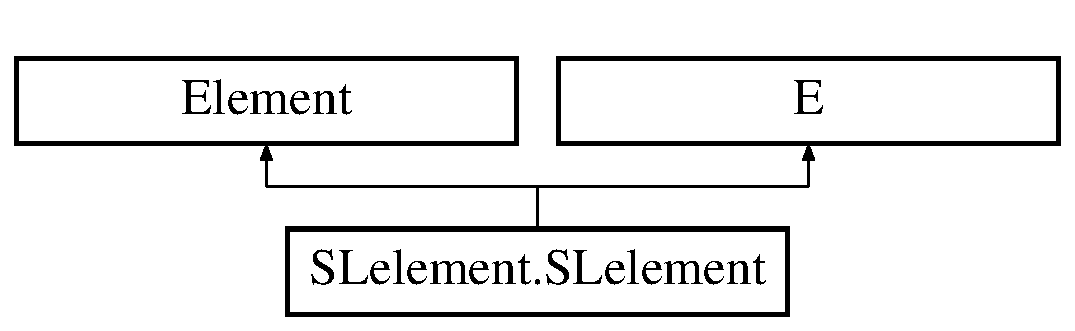
\includegraphics[height=4.912281cm]{class_s_lelement_1_1_s_lelement}
\end{center}
\end{figure}
\subsection*{Public Member Functions}
\begin{DoxyCompactItemize}
\item 
def \hyperlink{class_s_lelement_1_1_s_lelement_a36a0f938d36efd25969cc3828e6fee6e}{\+\_\+\+\_\+init\+\_\+\+\_\+}
\begin{DoxyCompactList}\small\item\em This constructor creates an \hyperlink{class_s_lelement_1_1_s_lelement}{S\+Lelement} object and sets the next pointer to null. \end{DoxyCompactList}\item 
def \hyperlink{class_s_lelement_1_1_s_lelement_af5ae396e58917855958c1599d70176ff}{get\+\_\+data\+\_\+structure\+\_\+type} (self)
\begin{DoxyCompactList}\small\item\em This method gets the data structure type. \end{DoxyCompactList}\item 
def \hyperlink{class_s_lelement_1_1_s_lelement_a2264429415080d591a53078c08c87eb4}{get\+\_\+next} (self)
\begin{DoxyCompactList}\small\item\em Retrieves the element following this element. \end{DoxyCompactList}\item 
def \hyperlink{class_s_lelement_1_1_s_lelement_a4cf835c80a52081242df0b8781234b63}{get\+\_\+value} (self)
\item 
def \hyperlink{class_s_lelement_1_1_s_lelement_ad984698ab1414df4d20fb083d619a2a8}{set\+\_\+next} (self, \hyperlink{class_s_lelement_1_1_s_lelement_a2d83afedba3b70183c90c3454ac99a29}{next})
\begin{DoxyCompactList}\small\item\em Sets the element to point to the next \hyperlink{class_s_lelement_1_1_s_lelement}{S\+Lelement}. \end{DoxyCompactList}\item 
def \hyperlink{class_s_lelement_1_1_s_lelement_ac33402fd5847218346937547e451f52d}{\+\_\+\+\_\+str\+\_\+\+\_\+} (self)
\item 
def \hyperlink{class_s_lelement_1_1_s_lelement_ae7c2565d705d8a473d46755d59e6ee18}{get\+\_\+data\+\_\+structure\+\_\+representation} (self)
\begin{DoxyCompactList}\small\item\em Get the J\+S\+O\+N representation of the the data structure. \end{DoxyCompactList}\item 
def \hyperlink{class_s_lelement_1_1_s_lelement_ac896487658a566e4ebf62734cf252e8f}{get\+\_\+list\+\_\+elements} (self, nodes)
\begin{DoxyCompactList}\small\item\em Get the elements of the list. \end{DoxyCompactList}\end{DoxyCompactItemize}
\subsection*{Public Attributes}
\begin{DoxyCompactItemize}
\item 
\hyperlink{class_s_lelement_1_1_s_lelement_a2d83afedba3b70183c90c3454ac99a29}{next}
\end{DoxyCompactItemize}
\subsection*{Additional Inherited Members}


\subsection{Detailed Description}
This class can be used to instantiate Singly Linked Elements. 

This class extends \hyperlink{namespace_element}{Element} and takes a generic parameter $<$\+E$>$ representing application specific data. This element forms the basic building block for singly linked lists. Singly linked elements have a field pointing to the next element along the list.

\begin{DoxyVerb}Elements contain a visualizer (ElementVisualizer) object for setting visual
attributes (color, shape, opacity, size), necessary for displaying them in a
web browser.

Elements also have a LinkVisualizer object, that is used when they are linked to
another element, appropriate for setting link attributes, for instance, between
the current element and its next element.
\end{DoxyVerb}


\begin{DoxyAuthor}{Author}
Mihai Mehedint, Kalpathi Subramanian
\end{DoxyAuthor}
\begin{DoxyDate}{Date}
6/22/16, 1/7/17, 5/17/17
\end{DoxyDate}

\begin{DoxyParams}{Parameters}
{\em $<$\+E$>$} & The generic parameter object that is part of this element, representing application specific data.\\
\hline
\end{DoxyParams}
\begin{DoxySeeAlso}{See also}
Example Tutorial at ~\newline
 \href{http://bridgesuncc.github.io/Hello_World_Tutorials/SLL.html}{\tt http\+://bridgesuncc.\+github.\+io/\+Hello\+\_\+\+World\+\_\+\+Tutorials/\+S\+L\+L.\+html} 
\end{DoxySeeAlso}


\subsection{Constructor \& Destructor Documentation}
\hypertarget{class_s_lelement_1_1_s_lelement_a36a0f938d36efd25969cc3828e6fee6e}{}\index{S\+Lelement\+::\+S\+Lelement@{S\+Lelement\+::\+S\+Lelement}!\+\_\+\+\_\+init\+\_\+\+\_\+@{\+\_\+\+\_\+init\+\_\+\+\_\+}}
\index{\+\_\+\+\_\+init\+\_\+\+\_\+@{\+\_\+\+\_\+init\+\_\+\+\_\+}!S\+Lelement\+::\+S\+Lelement@{S\+Lelement\+::\+S\+Lelement}}
\subsubsection[{\+\_\+\+\_\+init\+\_\+\+\_\+}]{\setlength{\rightskip}{0pt plus 5cm}def S\+Lelement.\+S\+Lelement.\+\_\+\+\_\+init\+\_\+\+\_\+ (
\begin{DoxyParamCaption}
\item[{}]{self, }
\item[{}]{e = {\ttfamily None}, }
\item[{}]{label = {\ttfamily None}, }
\item[{}]{next = {\ttfamily None}}
\end{DoxyParamCaption}
)}\label{class_s_lelement_1_1_s_lelement_a36a0f938d36efd25969cc3828e6fee6e}


This constructor creates an \hyperlink{class_s_lelement_1_1_s_lelement}{S\+Lelement} object and sets the next pointer to null. 



\subsection{Member Function Documentation}
\hypertarget{class_s_lelement_1_1_s_lelement_ac33402fd5847218346937547e451f52d}{}\index{S\+Lelement\+::\+S\+Lelement@{S\+Lelement\+::\+S\+Lelement}!\+\_\+\+\_\+str\+\_\+\+\_\+@{\+\_\+\+\_\+str\+\_\+\+\_\+}}
\index{\+\_\+\+\_\+str\+\_\+\+\_\+@{\+\_\+\+\_\+str\+\_\+\+\_\+}!S\+Lelement\+::\+S\+Lelement@{S\+Lelement\+::\+S\+Lelement}}
\subsubsection[{\+\_\+\+\_\+str\+\_\+\+\_\+(self)}]{\setlength{\rightskip}{0pt plus 5cm}def S\+Lelement.\+S\+Lelement.\+\_\+\+\_\+str\+\_\+\+\_\+ (
\begin{DoxyParamCaption}
\item[{}]{self}
\end{DoxyParamCaption}
)}\label{class_s_lelement_1_1_s_lelement_ac33402fd5847218346937547e451f52d}
\hypertarget{class_s_lelement_1_1_s_lelement_ae7c2565d705d8a473d46755d59e6ee18}{}\index{S\+Lelement\+::\+S\+Lelement@{S\+Lelement\+::\+S\+Lelement}!get\+\_\+data\+\_\+structure\+\_\+representation@{get\+\_\+data\+\_\+structure\+\_\+representation}}
\index{get\+\_\+data\+\_\+structure\+\_\+representation@{get\+\_\+data\+\_\+structure\+\_\+representation}!S\+Lelement\+::\+S\+Lelement@{S\+Lelement\+::\+S\+Lelement}}
\subsubsection[{get\+\_\+data\+\_\+structure\+\_\+representation(self)}]{\setlength{\rightskip}{0pt plus 5cm}def S\+Lelement.\+S\+Lelement.\+get\+\_\+data\+\_\+structure\+\_\+representation (
\begin{DoxyParamCaption}
\item[{}]{self}
\end{DoxyParamCaption}
)}\label{class_s_lelement_1_1_s_lelement_ae7c2565d705d8a473d46755d59e6ee18}


Get the J\+S\+O\+N representation of the the data structure. 

\hypertarget{class_s_lelement_1_1_s_lelement_af5ae396e58917855958c1599d70176ff}{}\index{S\+Lelement\+::\+S\+Lelement@{S\+Lelement\+::\+S\+Lelement}!get\+\_\+data\+\_\+structure\+\_\+type@{get\+\_\+data\+\_\+structure\+\_\+type}}
\index{get\+\_\+data\+\_\+structure\+\_\+type@{get\+\_\+data\+\_\+structure\+\_\+type}!S\+Lelement\+::\+S\+Lelement@{S\+Lelement\+::\+S\+Lelement}}
\subsubsection[{get\+\_\+data\+\_\+structure\+\_\+type(self)}]{\setlength{\rightskip}{0pt plus 5cm}def S\+Lelement.\+S\+Lelement.\+get\+\_\+data\+\_\+structure\+\_\+type (
\begin{DoxyParamCaption}
\item[{}]{self}
\end{DoxyParamCaption}
)}\label{class_s_lelement_1_1_s_lelement_af5ae396e58917855958c1599d70176ff}


This method gets the data structure type. 

\begin{DoxyReturn}{Returns}
The date structure type as a string 
\end{DoxyReturn}
\hypertarget{class_s_lelement_1_1_s_lelement_ac896487658a566e4ebf62734cf252e8f}{}\index{S\+Lelement\+::\+S\+Lelement@{S\+Lelement\+::\+S\+Lelement}!get\+\_\+list\+\_\+elements@{get\+\_\+list\+\_\+elements}}
\index{get\+\_\+list\+\_\+elements@{get\+\_\+list\+\_\+elements}!S\+Lelement\+::\+S\+Lelement@{S\+Lelement\+::\+S\+Lelement}}
\subsubsection[{get\+\_\+list\+\_\+elements(self, nodes)}]{\setlength{\rightskip}{0pt plus 5cm}def S\+Lelement.\+S\+Lelement.\+get\+\_\+list\+\_\+elements (
\begin{DoxyParamCaption}
\item[{}]{self, }
\item[{}]{nodes}
\end{DoxyParamCaption}
)}\label{class_s_lelement_1_1_s_lelement_ac896487658a566e4ebf62734cf252e8f}


Get the elements of the list. 


\begin{DoxyParams}{Parameters}
{\em nodes} & a vector of the ndoes in the list \\
\hline
\end{DoxyParams}
\hypertarget{class_s_lelement_1_1_s_lelement_a2264429415080d591a53078c08c87eb4}{}\index{S\+Lelement\+::\+S\+Lelement@{S\+Lelement\+::\+S\+Lelement}!get\+\_\+next@{get\+\_\+next}}
\index{get\+\_\+next@{get\+\_\+next}!S\+Lelement\+::\+S\+Lelement@{S\+Lelement\+::\+S\+Lelement}}
\subsubsection[{get\+\_\+next(self)}]{\setlength{\rightskip}{0pt plus 5cm}def S\+Lelement.\+S\+Lelement.\+get\+\_\+next (
\begin{DoxyParamCaption}
\item[{}]{self}
\end{DoxyParamCaption}
)}\label{class_s_lelement_1_1_s_lelement_a2264429415080d591a53078c08c87eb4}


Retrieves the element following this element. 

\begin{DoxyReturn}{Returns}
S\+Lelement$<$\+E$>$ assigned to next 
\end{DoxyReturn}
\hypertarget{class_s_lelement_1_1_s_lelement_a4cf835c80a52081242df0b8781234b63}{}\index{S\+Lelement\+::\+S\+Lelement@{S\+Lelement\+::\+S\+Lelement}!get\+\_\+value@{get\+\_\+value}}
\index{get\+\_\+value@{get\+\_\+value}!S\+Lelement\+::\+S\+Lelement@{S\+Lelement\+::\+S\+Lelement}}
\subsubsection[{get\+\_\+value(self)}]{\setlength{\rightskip}{0pt plus 5cm}def S\+Lelement.\+S\+Lelement.\+get\+\_\+value (
\begin{DoxyParamCaption}
\item[{}]{self}
\end{DoxyParamCaption}
)}\label{class_s_lelement_1_1_s_lelement_a4cf835c80a52081242df0b8781234b63}
\hypertarget{class_s_lelement_1_1_s_lelement_ad984698ab1414df4d20fb083d619a2a8}{}\index{S\+Lelement\+::\+S\+Lelement@{S\+Lelement\+::\+S\+Lelement}!set\+\_\+next@{set\+\_\+next}}
\index{set\+\_\+next@{set\+\_\+next}!S\+Lelement\+::\+S\+Lelement@{S\+Lelement\+::\+S\+Lelement}}
\subsubsection[{set\+\_\+next(self, next)}]{\setlength{\rightskip}{0pt plus 5cm}def S\+Lelement.\+S\+Lelement.\+set\+\_\+next (
\begin{DoxyParamCaption}
\item[{}]{self, }
\item[{}]{next}
\end{DoxyParamCaption}
)}\label{class_s_lelement_1_1_s_lelement_ad984698ab1414df4d20fb083d619a2a8}


Sets the element to point to the next \hyperlink{class_s_lelement_1_1_s_lelement}{S\+Lelement}. 


\begin{DoxyParams}{Parameters}
{\em next} & S\+Lelement$<$\+E$>$ that should be assigned to the next pointer \\
\hline
\end{DoxyParams}


\subsection{Member Data Documentation}
\hypertarget{class_s_lelement_1_1_s_lelement_a2d83afedba3b70183c90c3454ac99a29}{}\index{S\+Lelement\+::\+S\+Lelement@{S\+Lelement\+::\+S\+Lelement}!next@{next}}
\index{next@{next}!S\+Lelement\+::\+S\+Lelement@{S\+Lelement\+::\+S\+Lelement}}
\subsubsection[{next}]{\setlength{\rightskip}{0pt plus 5cm}S\+Lelement.\+S\+Lelement.\+next}\label{class_s_lelement_1_1_s_lelement_a2d83afedba3b70183c90c3454ac99a29}


The documentation for this class was generated from the following file\+:\begin{DoxyCompactItemize}
\item 
/\+Users/krs/gr/bridges/bridges17/python/src/\hyperlink{_s_lelement_8py}{S\+Lelement.\+py}\end{DoxyCompactItemize}

\hypertarget{class_song_1_1_song}{}\section{Song.\+Song Class Reference}
\label{class_song_1_1_song}\index{Song.\+Song@{Song.\+Song}}
\subsection*{Public Member Functions}
\begin{DoxyCompactItemize}
\item 
def \hyperlink{class_song_1_1_song_a7c712398cc9d5baf8e6f09f4c3918908}{\+\_\+\+\_\+init\+\_\+\+\_\+}
\item 
def \hyperlink{class_song_1_1_song_a62e7e0e4572b387a0c2af78e77dbe728}{get\+Artist} (self)
\item 
def \hyperlink{class_song_1_1_song_a05f3a6402149c46f1443e2fa0b6522b4}{set\+Artist} (self, \hyperlink{class_song_1_1_song_a43f00a67117668a929591164817c0183}{artist})
\item 
def \hyperlink{class_song_1_1_song_ab0f1fd5bf24722e8bed3a76cf63fa5a0}{get\+Song\+Title} (self)
\item 
def \hyperlink{class_song_1_1_song_ab3915e63c2a624e69cf7d3d0e771b960}{set\+Song\+Title} (self, \hyperlink{class_song_1_1_song_ace7c0f2f4985b73383d754c73caef745}{song})
\item 
def \hyperlink{class_song_1_1_song_a8f49c51da7549925fbe53332c9e7c150}{get\+Album\+Title} (self)
\item 
def \hyperlink{class_song_1_1_song_ad60c9bb355ef99775c11f98e99d09d97}{set\+Album\+Title} (self, \hyperlink{class_song_1_1_song_ad0d1e6cf79e3730a30231e799b880444}{album})
\item 
def \hyperlink{class_song_1_1_song_a06ba442bbf891e9d0e6955231327e46c}{get\+Lyrics} (self)
\item 
def \hyperlink{class_song_1_1_song_a21be1669f271664cc45f5f3695ea6efa}{set\+Lyrics} (self, \hyperlink{class_song_1_1_song_a615d9c5a45416c8bc394f0f8933ea01b}{lyrics})
\item 
def \hyperlink{class_song_1_1_song_a7f932d10de6f5873a9b257c1de00f0b7}{get\+Release\+Date} (self)
\item 
def \hyperlink{class_song_1_1_song_abc2cbaf2d3b19a7e58d3a11a5c5f494d}{set\+Release\+Date} (self, date)
\end{DoxyCompactItemize}
\subsection*{Public Attributes}
\begin{DoxyCompactItemize}
\item 
\hyperlink{class_song_1_1_song_a43f00a67117668a929591164817c0183}{artist}
\item 
\hyperlink{class_song_1_1_song_ace7c0f2f4985b73383d754c73caef745}{song}
\item 
\hyperlink{class_song_1_1_song_a615d9c5a45416c8bc394f0f8933ea01b}{lyrics}
\item 
\hyperlink{class_song_1_1_song_ad0d1e6cf79e3730a30231e799b880444}{album}
\item 
\hyperlink{class_song_1_1_song_ae8e1db27b18ac777478522a33fb2a611}{release\+\_\+date}
\end{DoxyCompactItemize}


\subsection{Constructor \& Destructor Documentation}
\hypertarget{class_song_1_1_song_a7c712398cc9d5baf8e6f09f4c3918908}{}\index{Song\+::\+Song@{Song\+::\+Song}!\+\_\+\+\_\+init\+\_\+\+\_\+@{\+\_\+\+\_\+init\+\_\+\+\_\+}}
\index{\+\_\+\+\_\+init\+\_\+\+\_\+@{\+\_\+\+\_\+init\+\_\+\+\_\+}!Song\+::\+Song@{Song\+::\+Song}}
\subsubsection[{\+\_\+\+\_\+init\+\_\+\+\_\+}]{\setlength{\rightskip}{0pt plus 5cm}def Song.\+Song.\+\_\+\+\_\+init\+\_\+\+\_\+ (
\begin{DoxyParamCaption}
\item[{}]{self, }
\item[{}]{artist = {\ttfamily None}, }
\item[{}]{song = {\ttfamily None}, }
\item[{}]{album = {\ttfamily None}, }
\item[{}]{lyrics = {\ttfamily None}, }
\item[{}]{release\+\_\+date = {\ttfamily None}}
\end{DoxyParamCaption}
)}\label{class_song_1_1_song_a7c712398cc9d5baf8e6f09f4c3918908}


\subsection{Member Function Documentation}
\hypertarget{class_song_1_1_song_a8f49c51da7549925fbe53332c9e7c150}{}\index{Song\+::\+Song@{Song\+::\+Song}!get\+Album\+Title@{get\+Album\+Title}}
\index{get\+Album\+Title@{get\+Album\+Title}!Song\+::\+Song@{Song\+::\+Song}}
\subsubsection[{get\+Album\+Title(self)}]{\setlength{\rightskip}{0pt plus 5cm}def Song.\+Song.\+get\+Album\+Title (
\begin{DoxyParamCaption}
\item[{}]{self}
\end{DoxyParamCaption}
)}\label{class_song_1_1_song_a8f49c51da7549925fbe53332c9e7c150}
\hypertarget{class_song_1_1_song_a62e7e0e4572b387a0c2af78e77dbe728}{}\index{Song\+::\+Song@{Song\+::\+Song}!get\+Artist@{get\+Artist}}
\index{get\+Artist@{get\+Artist}!Song\+::\+Song@{Song\+::\+Song}}
\subsubsection[{get\+Artist(self)}]{\setlength{\rightskip}{0pt plus 5cm}def Song.\+Song.\+get\+Artist (
\begin{DoxyParamCaption}
\item[{}]{self}
\end{DoxyParamCaption}
)}\label{class_song_1_1_song_a62e7e0e4572b387a0c2af78e77dbe728}
\hypertarget{class_song_1_1_song_a06ba442bbf891e9d0e6955231327e46c}{}\index{Song\+::\+Song@{Song\+::\+Song}!get\+Lyrics@{get\+Lyrics}}
\index{get\+Lyrics@{get\+Lyrics}!Song\+::\+Song@{Song\+::\+Song}}
\subsubsection[{get\+Lyrics(self)}]{\setlength{\rightskip}{0pt plus 5cm}def Song.\+Song.\+get\+Lyrics (
\begin{DoxyParamCaption}
\item[{}]{self}
\end{DoxyParamCaption}
)}\label{class_song_1_1_song_a06ba442bbf891e9d0e6955231327e46c}
\hypertarget{class_song_1_1_song_a7f932d10de6f5873a9b257c1de00f0b7}{}\index{Song\+::\+Song@{Song\+::\+Song}!get\+Release\+Date@{get\+Release\+Date}}
\index{get\+Release\+Date@{get\+Release\+Date}!Song\+::\+Song@{Song\+::\+Song}}
\subsubsection[{get\+Release\+Date(self)}]{\setlength{\rightskip}{0pt plus 5cm}def Song.\+Song.\+get\+Release\+Date (
\begin{DoxyParamCaption}
\item[{}]{self}
\end{DoxyParamCaption}
)}\label{class_song_1_1_song_a7f932d10de6f5873a9b257c1de00f0b7}
\hypertarget{class_song_1_1_song_ab0f1fd5bf24722e8bed3a76cf63fa5a0}{}\index{Song\+::\+Song@{Song\+::\+Song}!get\+Song\+Title@{get\+Song\+Title}}
\index{get\+Song\+Title@{get\+Song\+Title}!Song\+::\+Song@{Song\+::\+Song}}
\subsubsection[{get\+Song\+Title(self)}]{\setlength{\rightskip}{0pt plus 5cm}def Song.\+Song.\+get\+Song\+Title (
\begin{DoxyParamCaption}
\item[{}]{self}
\end{DoxyParamCaption}
)}\label{class_song_1_1_song_ab0f1fd5bf24722e8bed3a76cf63fa5a0}
\hypertarget{class_song_1_1_song_ad60c9bb355ef99775c11f98e99d09d97}{}\index{Song\+::\+Song@{Song\+::\+Song}!set\+Album\+Title@{set\+Album\+Title}}
\index{set\+Album\+Title@{set\+Album\+Title}!Song\+::\+Song@{Song\+::\+Song}}
\subsubsection[{set\+Album\+Title(self, album)}]{\setlength{\rightskip}{0pt plus 5cm}def Song.\+Song.\+set\+Album\+Title (
\begin{DoxyParamCaption}
\item[{}]{self, }
\item[{}]{album}
\end{DoxyParamCaption}
)}\label{class_song_1_1_song_ad60c9bb355ef99775c11f98e99d09d97}
\hypertarget{class_song_1_1_song_a05f3a6402149c46f1443e2fa0b6522b4}{}\index{Song\+::\+Song@{Song\+::\+Song}!set\+Artist@{set\+Artist}}
\index{set\+Artist@{set\+Artist}!Song\+::\+Song@{Song\+::\+Song}}
\subsubsection[{set\+Artist(self, artist)}]{\setlength{\rightskip}{0pt plus 5cm}def Song.\+Song.\+set\+Artist (
\begin{DoxyParamCaption}
\item[{}]{self, }
\item[{}]{artist}
\end{DoxyParamCaption}
)}\label{class_song_1_1_song_a05f3a6402149c46f1443e2fa0b6522b4}
\hypertarget{class_song_1_1_song_a21be1669f271664cc45f5f3695ea6efa}{}\index{Song\+::\+Song@{Song\+::\+Song}!set\+Lyrics@{set\+Lyrics}}
\index{set\+Lyrics@{set\+Lyrics}!Song\+::\+Song@{Song\+::\+Song}}
\subsubsection[{set\+Lyrics(self, lyrics)}]{\setlength{\rightskip}{0pt plus 5cm}def Song.\+Song.\+set\+Lyrics (
\begin{DoxyParamCaption}
\item[{}]{self, }
\item[{}]{lyrics}
\end{DoxyParamCaption}
)}\label{class_song_1_1_song_a21be1669f271664cc45f5f3695ea6efa}
\hypertarget{class_song_1_1_song_abc2cbaf2d3b19a7e58d3a11a5c5f494d}{}\index{Song\+::\+Song@{Song\+::\+Song}!set\+Release\+Date@{set\+Release\+Date}}
\index{set\+Release\+Date@{set\+Release\+Date}!Song\+::\+Song@{Song\+::\+Song}}
\subsubsection[{set\+Release\+Date(self, date)}]{\setlength{\rightskip}{0pt plus 5cm}def Song.\+Song.\+set\+Release\+Date (
\begin{DoxyParamCaption}
\item[{}]{self, }
\item[{}]{date}
\end{DoxyParamCaption}
)}\label{class_song_1_1_song_abc2cbaf2d3b19a7e58d3a11a5c5f494d}
\hypertarget{class_song_1_1_song_ab3915e63c2a624e69cf7d3d0e771b960}{}\index{Song\+::\+Song@{Song\+::\+Song}!set\+Song\+Title@{set\+Song\+Title}}
\index{set\+Song\+Title@{set\+Song\+Title}!Song\+::\+Song@{Song\+::\+Song}}
\subsubsection[{set\+Song\+Title(self, song)}]{\setlength{\rightskip}{0pt plus 5cm}def Song.\+Song.\+set\+Song\+Title (
\begin{DoxyParamCaption}
\item[{}]{self, }
\item[{}]{song}
\end{DoxyParamCaption}
)}\label{class_song_1_1_song_ab3915e63c2a624e69cf7d3d0e771b960}


\subsection{Member Data Documentation}
\hypertarget{class_song_1_1_song_ad0d1e6cf79e3730a30231e799b880444}{}\index{Song\+::\+Song@{Song\+::\+Song}!album@{album}}
\index{album@{album}!Song\+::\+Song@{Song\+::\+Song}}
\subsubsection[{album}]{\setlength{\rightskip}{0pt plus 5cm}Song.\+Song.\+album}\label{class_song_1_1_song_ad0d1e6cf79e3730a30231e799b880444}
\hypertarget{class_song_1_1_song_a43f00a67117668a929591164817c0183}{}\index{Song\+::\+Song@{Song\+::\+Song}!artist@{artist}}
\index{artist@{artist}!Song\+::\+Song@{Song\+::\+Song}}
\subsubsection[{artist}]{\setlength{\rightskip}{0pt plus 5cm}Song.\+Song.\+artist}\label{class_song_1_1_song_a43f00a67117668a929591164817c0183}
\hypertarget{class_song_1_1_song_a615d9c5a45416c8bc394f0f8933ea01b}{}\index{Song\+::\+Song@{Song\+::\+Song}!lyrics@{lyrics}}
\index{lyrics@{lyrics}!Song\+::\+Song@{Song\+::\+Song}}
\subsubsection[{lyrics}]{\setlength{\rightskip}{0pt plus 5cm}Song.\+Song.\+lyrics}\label{class_song_1_1_song_a615d9c5a45416c8bc394f0f8933ea01b}
\hypertarget{class_song_1_1_song_ae8e1db27b18ac777478522a33fb2a611}{}\index{Song\+::\+Song@{Song\+::\+Song}!release\+\_\+date@{release\+\_\+date}}
\index{release\+\_\+date@{release\+\_\+date}!Song\+::\+Song@{Song\+::\+Song}}
\subsubsection[{release\+\_\+date}]{\setlength{\rightskip}{0pt plus 5cm}Song.\+Song.\+release\+\_\+date}\label{class_song_1_1_song_ae8e1db27b18ac777478522a33fb2a611}
\hypertarget{class_song_1_1_song_ace7c0f2f4985b73383d754c73caef745}{}\index{Song\+::\+Song@{Song\+::\+Song}!song@{song}}
\index{song@{song}!Song\+::\+Song@{Song\+::\+Song}}
\subsubsection[{song}]{\setlength{\rightskip}{0pt plus 5cm}Song.\+Song.\+song}\label{class_song_1_1_song_ace7c0f2f4985b73383d754c73caef745}


The documentation for this class was generated from the following file\+:\begin{DoxyCompactItemize}
\item 
/\+Users/krs/gr/bridges/bridges17/python/src/data\+\_\+src\+\_\+dependent/\hyperlink{_song_8py}{Song.\+py}\end{DoxyCompactItemize}

\hypertarget{class_student_1_1_student}{}\section{Student.\+Student Class Reference}
\label{class_student_1_1_student}\index{Student.\+Student@{Student.\+Student}}
\subsection*{Public Member Functions}
\begin{DoxyCompactItemize}
\item 
def \hyperlink{class_student_1_1_student_a8069666ff37178cf2cf5f72792331ad4}{\+\_\+\+\_\+init\+\_\+\+\_\+} (self, \hyperlink{class_student_1_1_student_ad0ff2ef29969f92c737112ff76e1eb23}{student\+I\+D}, \hyperlink{class_student_1_1_student_a6377fa53bde2bd9a09402417a970cfe0}{full\+Name}, \hyperlink{class_student_1_1_student_afef32339c4759ebe384fa3fe43e0f947}{program}, \hyperlink{class_student_1_1_student_a15646360e956aadb3d60f00795d2190e}{email}, \hyperlink{class_student_1_1_student_ace53802842808ff3f2eca0702e6dec28}{dislike\+Color}, \hyperlink{class_student_1_1_student_a0225aab3458da940a21b332cdcba3fce}{favorite\+Color}, \hyperlink{class_student_1_1_student_a7500ff9d6e8b1e9795aadbf6b375ae59}{student\+Credit\+Hours})
\end{DoxyCompactItemize}
\subsection*{Public Attributes}
\begin{DoxyCompactItemize}
\item 
\hyperlink{class_student_1_1_student_ae09b19677b0b71c7977702f7f85266f1}{student\+I\+D}
\item 
\hyperlink{class_student_1_1_student_a42c4e512c2ef23b9c3fbadb1463be825}{full\+Name}
\item 
\hyperlink{class_student_1_1_student_ac059f070275775de6e9f859d0927022e}{program}
\item 
\hyperlink{class_student_1_1_student_a136f11ba8b93b9c445e32acf8769f301}{email}
\item 
\hyperlink{class_student_1_1_student_ab15343e6ee78653c95b64937395048b2}{dislike\+Color}
\item 
\hyperlink{class_student_1_1_student_a3b4a68fc25418358f8c7eaac45bcb0a5}{favorite\+Color}
\item 
\hyperlink{class_student_1_1_student_ae2833e95922c2320ceade64dee9b66d0}{student\+Credit\+Hours}
\end{DoxyCompactItemize}
\subsection*{Static Public Attributes}
\begin{DoxyCompactItemize}
\item 
tuple \hyperlink{class_student_1_1_student_ad0ff2ef29969f92c737112ff76e1eb23}{student\+I\+D} = str()
\item 
tuple \hyperlink{class_student_1_1_student_a6377fa53bde2bd9a09402417a970cfe0}{full\+Name} = str()
\item 
tuple \hyperlink{class_student_1_1_student_afef32339c4759ebe384fa3fe43e0f947}{program} = str()
\item 
tuple \hyperlink{class_student_1_1_student_a15646360e956aadb3d60f00795d2190e}{email} = str()
\item 
tuple \hyperlink{class_student_1_1_student_ace53802842808ff3f2eca0702e6dec28}{dislike\+Color} = str()
\item 
tuple \hyperlink{class_student_1_1_student_a0225aab3458da940a21b332cdcba3fce}{favorite\+Color} = str()
\item 
tuple \hyperlink{class_student_1_1_student_a7500ff9d6e8b1e9795aadbf6b375ae59}{student\+Credit\+Hours} = float()
\end{DoxyCompactItemize}


\subsection{Constructor \& Destructor Documentation}
\hypertarget{class_student_1_1_student_a8069666ff37178cf2cf5f72792331ad4}{}\index{Student\+::\+Student@{Student\+::\+Student}!\+\_\+\+\_\+init\+\_\+\+\_\+@{\+\_\+\+\_\+init\+\_\+\+\_\+}}
\index{\+\_\+\+\_\+init\+\_\+\+\_\+@{\+\_\+\+\_\+init\+\_\+\+\_\+}!Student\+::\+Student@{Student\+::\+Student}}
\subsubsection[{\+\_\+\+\_\+init\+\_\+\+\_\+(self, student\+I\+D, full\+Name, program, email, dislike\+Color, favorite\+Color, student\+Credit\+Hours)}]{\setlength{\rightskip}{0pt plus 5cm}def Student.\+Student.\+\_\+\+\_\+init\+\_\+\+\_\+ (
\begin{DoxyParamCaption}
\item[{}]{self, }
\item[{}]{student\+I\+D, }
\item[{}]{full\+Name, }
\item[{}]{program, }
\item[{}]{email, }
\item[{}]{dislike\+Color, }
\item[{}]{favorite\+Color, }
\item[{}]{student\+Credit\+Hours}
\end{DoxyParamCaption}
)}\label{class_student_1_1_student_a8069666ff37178cf2cf5f72792331ad4}


\subsection{Member Data Documentation}
\hypertarget{class_student_1_1_student_ace53802842808ff3f2eca0702e6dec28}{}\index{Student\+::\+Student@{Student\+::\+Student}!dislike\+Color@{dislike\+Color}}
\index{dislike\+Color@{dislike\+Color}!Student\+::\+Student@{Student\+::\+Student}}
\subsubsection[{dislike\+Color}]{\setlength{\rightskip}{0pt plus 5cm}tuple Student.\+Student.\+dislike\+Color = str()\hspace{0.3cm}{\ttfamily [static]}}\label{class_student_1_1_student_ace53802842808ff3f2eca0702e6dec28}
\hypertarget{class_student_1_1_student_ab15343e6ee78653c95b64937395048b2}{}\index{Student\+::\+Student@{Student\+::\+Student}!dislike\+Color@{dislike\+Color}}
\index{dislike\+Color@{dislike\+Color}!Student\+::\+Student@{Student\+::\+Student}}
\subsubsection[{dislike\+Color}]{\setlength{\rightskip}{0pt plus 5cm}Student.\+Student.\+dislike\+Color}\label{class_student_1_1_student_ab15343e6ee78653c95b64937395048b2}
\hypertarget{class_student_1_1_student_a15646360e956aadb3d60f00795d2190e}{}\index{Student\+::\+Student@{Student\+::\+Student}!email@{email}}
\index{email@{email}!Student\+::\+Student@{Student\+::\+Student}}
\subsubsection[{email}]{\setlength{\rightskip}{0pt plus 5cm}tuple Student.\+Student.\+email = str()\hspace{0.3cm}{\ttfamily [static]}}\label{class_student_1_1_student_a15646360e956aadb3d60f00795d2190e}
\hypertarget{class_student_1_1_student_a136f11ba8b93b9c445e32acf8769f301}{}\index{Student\+::\+Student@{Student\+::\+Student}!email@{email}}
\index{email@{email}!Student\+::\+Student@{Student\+::\+Student}}
\subsubsection[{email}]{\setlength{\rightskip}{0pt plus 5cm}Student.\+Student.\+email}\label{class_student_1_1_student_a136f11ba8b93b9c445e32acf8769f301}
\hypertarget{class_student_1_1_student_a0225aab3458da940a21b332cdcba3fce}{}\index{Student\+::\+Student@{Student\+::\+Student}!favorite\+Color@{favorite\+Color}}
\index{favorite\+Color@{favorite\+Color}!Student\+::\+Student@{Student\+::\+Student}}
\subsubsection[{favorite\+Color}]{\setlength{\rightskip}{0pt plus 5cm}tuple Student.\+Student.\+favorite\+Color = str()\hspace{0.3cm}{\ttfamily [static]}}\label{class_student_1_1_student_a0225aab3458da940a21b332cdcba3fce}
\hypertarget{class_student_1_1_student_a3b4a68fc25418358f8c7eaac45bcb0a5}{}\index{Student\+::\+Student@{Student\+::\+Student}!favorite\+Color@{favorite\+Color}}
\index{favorite\+Color@{favorite\+Color}!Student\+::\+Student@{Student\+::\+Student}}
\subsubsection[{favorite\+Color}]{\setlength{\rightskip}{0pt plus 5cm}Student.\+Student.\+favorite\+Color}\label{class_student_1_1_student_a3b4a68fc25418358f8c7eaac45bcb0a5}
\hypertarget{class_student_1_1_student_a6377fa53bde2bd9a09402417a970cfe0}{}\index{Student\+::\+Student@{Student\+::\+Student}!full\+Name@{full\+Name}}
\index{full\+Name@{full\+Name}!Student\+::\+Student@{Student\+::\+Student}}
\subsubsection[{full\+Name}]{\setlength{\rightskip}{0pt plus 5cm}tuple Student.\+Student.\+full\+Name = str()\hspace{0.3cm}{\ttfamily [static]}}\label{class_student_1_1_student_a6377fa53bde2bd9a09402417a970cfe0}
\hypertarget{class_student_1_1_student_a42c4e512c2ef23b9c3fbadb1463be825}{}\index{Student\+::\+Student@{Student\+::\+Student}!full\+Name@{full\+Name}}
\index{full\+Name@{full\+Name}!Student\+::\+Student@{Student\+::\+Student}}
\subsubsection[{full\+Name}]{\setlength{\rightskip}{0pt plus 5cm}Student.\+Student.\+full\+Name}\label{class_student_1_1_student_a42c4e512c2ef23b9c3fbadb1463be825}
\hypertarget{class_student_1_1_student_afef32339c4759ebe384fa3fe43e0f947}{}\index{Student\+::\+Student@{Student\+::\+Student}!program@{program}}
\index{program@{program}!Student\+::\+Student@{Student\+::\+Student}}
\subsubsection[{program}]{\setlength{\rightskip}{0pt plus 5cm}tuple Student.\+Student.\+program = str()\hspace{0.3cm}{\ttfamily [static]}}\label{class_student_1_1_student_afef32339c4759ebe384fa3fe43e0f947}
\hypertarget{class_student_1_1_student_ac059f070275775de6e9f859d0927022e}{}\index{Student\+::\+Student@{Student\+::\+Student}!program@{program}}
\index{program@{program}!Student\+::\+Student@{Student\+::\+Student}}
\subsubsection[{program}]{\setlength{\rightskip}{0pt plus 5cm}Student.\+Student.\+program}\label{class_student_1_1_student_ac059f070275775de6e9f859d0927022e}
\hypertarget{class_student_1_1_student_a7500ff9d6e8b1e9795aadbf6b375ae59}{}\index{Student\+::\+Student@{Student\+::\+Student}!student\+Credit\+Hours@{student\+Credit\+Hours}}
\index{student\+Credit\+Hours@{student\+Credit\+Hours}!Student\+::\+Student@{Student\+::\+Student}}
\subsubsection[{student\+Credit\+Hours}]{\setlength{\rightskip}{0pt plus 5cm}tuple Student.\+Student.\+student\+Credit\+Hours = float()\hspace{0.3cm}{\ttfamily [static]}}\label{class_student_1_1_student_a7500ff9d6e8b1e9795aadbf6b375ae59}
\hypertarget{class_student_1_1_student_ae2833e95922c2320ceade64dee9b66d0}{}\index{Student\+::\+Student@{Student\+::\+Student}!student\+Credit\+Hours@{student\+Credit\+Hours}}
\index{student\+Credit\+Hours@{student\+Credit\+Hours}!Student\+::\+Student@{Student\+::\+Student}}
\subsubsection[{student\+Credit\+Hours}]{\setlength{\rightskip}{0pt plus 5cm}Student.\+Student.\+student\+Credit\+Hours}\label{class_student_1_1_student_ae2833e95922c2320ceade64dee9b66d0}
\hypertarget{class_student_1_1_student_ad0ff2ef29969f92c737112ff76e1eb23}{}\index{Student\+::\+Student@{Student\+::\+Student}!student\+I\+D@{student\+I\+D}}
\index{student\+I\+D@{student\+I\+D}!Student\+::\+Student@{Student\+::\+Student}}
\subsubsection[{student\+I\+D}]{\setlength{\rightskip}{0pt plus 5cm}tuple Student.\+Student.\+student\+I\+D = str()\hspace{0.3cm}{\ttfamily [static]}}\label{class_student_1_1_student_ad0ff2ef29969f92c737112ff76e1eb23}
\hypertarget{class_student_1_1_student_ae09b19677b0b71c7977702f7f85266f1}{}\index{Student\+::\+Student@{Student\+::\+Student}!student\+I\+D@{student\+I\+D}}
\index{student\+I\+D@{student\+I\+D}!Student\+::\+Student@{Student\+::\+Student}}
\subsubsection[{student\+I\+D}]{\setlength{\rightskip}{0pt plus 5cm}Student.\+Student.\+student\+I\+D}\label{class_student_1_1_student_ae09b19677b0b71c7977702f7f85266f1}


The documentation for this class was generated from the following file\+:\begin{DoxyCompactItemize}
\item 
/\+Users/krs/gr/bridges/bridges17/python/src/\hyperlink{_student_8py}{Student.\+py}\end{DoxyCompactItemize}

\hypertarget{class_tree_element_1_1_tree_element}{}\section{Tree\+Element.\+Tree\+Element Class Reference}
\label{class_tree_element_1_1_tree_element}\index{Tree\+Element.\+Tree\+Element@{Tree\+Element.\+Tree\+Element}}


This class extends \hyperlink{namespace_element}{Element} to represent general trees with arbitrary number of children.  


Inheritance diagram for Tree\+Element.\+Tree\+Element\+:\begin{figure}[H]
\begin{center}
\leavevmode
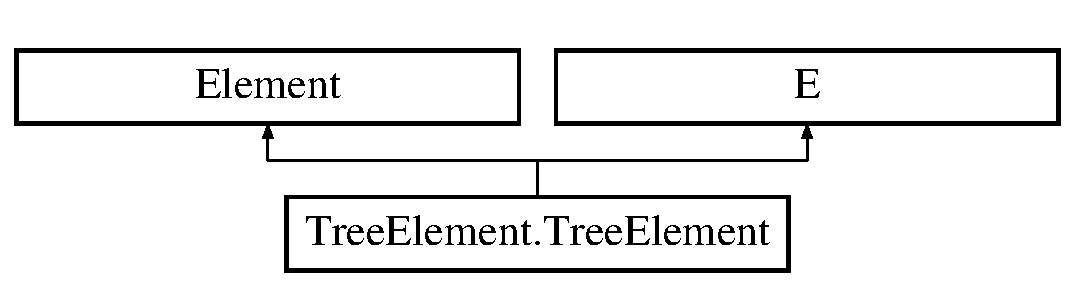
\includegraphics[height=6.000000cm]{class_tree_element_1_1_tree_element}
\end{center}
\end{figure}
\subsection*{Public Member Functions}
\begin{DoxyCompactItemize}
\item 
def \hyperlink{class_tree_element_1_1_tree_element_aa723139eac741f5e4318c0e546511272}{\+\_\+\+\_\+init\+\_\+\+\_\+}
\begin{DoxyCompactList}\small\item\em Constructs an empty \hyperlink{class_tree_element_1_1_tree_element}{Tree\+Element} with first two children set to null. \end{DoxyCompactList}\item 
def \hyperlink{class_tree_element_1_1_tree_element_a524729eed4d8a0ba3dc9e857777f3fd3}{get\+\_\+data\+\_\+structure\+\_\+type} (self)
\begin{DoxyCompactList}\small\item\em This method gets the data structure type. \end{DoxyCompactList}\item 
def \hyperlink{class_tree_element_1_1_tree_element_a472f1d0d906f4a8a8c48a54d83d42fd5}{add\+\_\+child} (self, child)
\begin{DoxyCompactList}\small\item\em Adds a child to the node. \end{DoxyCompactList}\item 
def \hyperlink{class_tree_element_1_1_tree_element_a8e5eb2215d0eaddf851cf2e3cbd2483b}{get\+\_\+number\+\_\+of\+\_\+children} (self)
\begin{DoxyCompactList}\small\item\em Returns the number of children at this node. \end{DoxyCompactList}\item 
def \hyperlink{class_tree_element_1_1_tree_element_a9a4b8a9c36075af52feea0b227ddac17}{set\+\_\+child} (self, index, child)
\begin{DoxyCompactList}\small\item\em adds a child to the node -\/ will be added at the next open position \end{DoxyCompactList}\item 
def \hyperlink{class_tree_element_1_1_tree_element_a242942c3685752b9ad29bd73a9200b59}{get\+\_\+child} (self, index)
\begin{DoxyCompactList}\small\item\em gets a child at a particular index \end{DoxyCompactList}\item 
def \hyperlink{class_tree_element_1_1_tree_element_a5df7317f551287a4ed0648887e0c168c}{get\+\_\+data\+\_\+structure\+\_\+representation} (self)
\begin{DoxyCompactList}\small\item\em Get hierarchical J\+S\+O\+N of the tree representation. \end{DoxyCompactList}\item 
def \hyperlink{class_tree_element_1_1_tree_element_a5bb802d6c08f735a35ae742d6fef5b4b}{pre\+\_\+order} (self, root)
\begin{DoxyCompactList}\small\item\em Use a preorder traversal to directly extract a hierarchical J\+S\+O\+N representation of the tree. \end{DoxyCompactList}\end{DoxyCompactItemize}
\subsection*{Public Attributes}
\begin{DoxyCompactItemize}
\item 
\hyperlink{class_tree_element_1_1_tree_element_aebd379cad696c2537f6a055f087b906a}{children}
\end{DoxyCompactItemize}
\subsection*{Static Public Attributes}
\begin{DoxyCompactItemize}
\item 
list \hyperlink{class_tree_element_1_1_tree_element_ae0cb830d32da4af3e42635bc541c0d5d}{children} = \mbox{[}$\,$\mbox{]}
\begin{DoxyCompactList}\small\item\em holds all children of the node \end{DoxyCompactList}\item 
string \hyperlink{class_tree_element_1_1_tree_element_a65174e78fa3608767a4c39e3a57b3e7b}{Q\+U\+O\+T\+E} = \char`\"{}\textbackslash{}\char`\"{}\char`\"{}
\item 
string \hyperlink{class_tree_element_1_1_tree_element_a7c60e7e6b2932c777ff04e10a3743e71}{C\+O\+M\+M\+A} = \char`\"{},\char`\"{}
\item 
string \hyperlink{class_tree_element_1_1_tree_element_a969eb933243a09855f14255eaf4d277f}{C\+O\+L\+O\+N} = \char`\"{}\+:\char`\"{}
\item 
string \hyperlink{class_tree_element_1_1_tree_element_a8527e74740e4c2e04fdd4387f1cc89a9}{O\+P\+E\+N\+\_\+\+C\+U\+R\+L\+Y} = \char`\"{}\{\char`\"{}
\item 
string \hyperlink{class_tree_element_1_1_tree_element_a292bcded0f33007fa75ef0b9df22c268}{C\+L\+O\+S\+E\+\_\+\+C\+U\+R\+L\+Y} = \char`\"{}\}\char`\"{}
\item 
string \hyperlink{class_tree_element_1_1_tree_element_a543ac127f5fe123828075efe7de84eef}{O\+P\+E\+N\+\_\+\+P\+A\+R\+E\+N} = \char`\"{}(\char`\"{}
\item 
string \hyperlink{class_tree_element_1_1_tree_element_ae091d14c49001870c4ed738f363e1d3c}{C\+L\+O\+S\+E\+\_\+\+P\+A\+R\+E\+N} = \char`\"{})\char`\"{}
\item 
string \hyperlink{class_tree_element_1_1_tree_element_a0f49fc3331346c2ba3a8db5e50c1710a}{O\+P\+E\+N\+\_\+\+B\+O\+X} = \char`\"{}\mbox{[}\char`\"{}
\item 
string \hyperlink{class_tree_element_1_1_tree_element_a55eef8f9bbd59e13882c40d636e112cc}{C\+L\+O\+S\+E\+\_\+\+B\+O\+X} = \char`\"{}\mbox{]}\char`\"{}
\end{DoxyCompactItemize}


\subsection{Detailed Description}
This class extends \hyperlink{namespace_element}{Element} to represent general trees with arbitrary number of children. 

\hyperlink{class_tree_element_1_1_tree_element}{Tree\+Element} nodes can have an arbitrary number of child nodes(held in in a vector in the order in which they were added). The visualization of trees assumes that the children are drawn in order from left to right.

Tree Elements have labels (string) that are displayed on the visualization. Elements take an generic object E as a user defined parameter, which can be any native type or object.

Elements contain a visualizer (\hyperlink{namespace_element_visualizer}{Element\+Visualizer}) object for setting visual attributes (color, shape, opacity, size), necessary for displaying them in a web browser.

Elements also have a \hyperlink{namespace_link_visualizer}{Link\+Visualizer} object that is used when they are linked to another element, appropriate for setting link attributes, between parent and child nodes.

\begin{DoxyAuthor}{Author}
Matthew Mc\+Quaigue
\end{DoxyAuthor}
\begin{DoxyDate}{Date}
12/16/17
\end{DoxyDate}

\begin{DoxyParams}{Parameters}
{\em $<$\+E$>$} & The generic parameter object that is part of this element, representing application specific data. \\
\hline
\end{DoxyParams}


\subsection{Constructor \& Destructor Documentation}
\hypertarget{class_tree_element_1_1_tree_element_aa723139eac741f5e4318c0e546511272}{}\index{Tree\+Element\+::\+Tree\+Element@{Tree\+Element\+::\+Tree\+Element}!\+\_\+\+\_\+init\+\_\+\+\_\+@{\+\_\+\+\_\+init\+\_\+\+\_\+}}
\index{\+\_\+\+\_\+init\+\_\+\+\_\+@{\+\_\+\+\_\+init\+\_\+\+\_\+}!Tree\+Element\+::\+Tree\+Element@{Tree\+Element\+::\+Tree\+Element}}
\subsubsection[{\+\_\+\+\_\+init\+\_\+\+\_\+}]{\setlength{\rightskip}{0pt plus 5cm}def Tree\+Element.\+Tree\+Element.\+\_\+\+\_\+init\+\_\+\+\_\+ (
\begin{DoxyParamCaption}
\item[{}]{self, }
\item[{}]{label = {\ttfamily None}, }
\item[{}]{e = {\ttfamily None}, }
\item[{}]{left = {\ttfamily None}, }
\item[{}]{right = {\ttfamily None}}
\end{DoxyParamCaption}
)}\label{class_tree_element_1_1_tree_element_aa723139eac741f5e4318c0e546511272}


Constructs an empty \hyperlink{class_tree_element_1_1_tree_element}{Tree\+Element} with first two children set to null. 



\subsection{Member Function Documentation}
\hypertarget{class_tree_element_1_1_tree_element_a472f1d0d906f4a8a8c48a54d83d42fd5}{}\index{Tree\+Element\+::\+Tree\+Element@{Tree\+Element\+::\+Tree\+Element}!add\+\_\+child@{add\+\_\+child}}
\index{add\+\_\+child@{add\+\_\+child}!Tree\+Element\+::\+Tree\+Element@{Tree\+Element\+::\+Tree\+Element}}
\subsubsection[{add\+\_\+child(self, child)}]{\setlength{\rightskip}{0pt plus 5cm}def Tree\+Element.\+Tree\+Element.\+add\+\_\+child (
\begin{DoxyParamCaption}
\item[{}]{self, }
\item[{}]{child}
\end{DoxyParamCaption}
)}\label{class_tree_element_1_1_tree_element_a472f1d0d906f4a8a8c48a54d83d42fd5}


Adds a child to the node. 

\hypertarget{class_tree_element_1_1_tree_element_a242942c3685752b9ad29bd73a9200b59}{}\index{Tree\+Element\+::\+Tree\+Element@{Tree\+Element\+::\+Tree\+Element}!get\+\_\+child@{get\+\_\+child}}
\index{get\+\_\+child@{get\+\_\+child}!Tree\+Element\+::\+Tree\+Element@{Tree\+Element\+::\+Tree\+Element}}
\subsubsection[{get\+\_\+child(self, index)}]{\setlength{\rightskip}{0pt plus 5cm}def Tree\+Element.\+Tree\+Element.\+get\+\_\+child (
\begin{DoxyParamCaption}
\item[{}]{self, }
\item[{}]{index}
\end{DoxyParamCaption}
)}\label{class_tree_element_1_1_tree_element_a242942c3685752b9ad29bd73a9200b59}


gets a child at a particular index 


\begin{DoxyParams}{Parameters}
{\em index} & into the list of children\\
\hline
\end{DoxyParams}
\begin{DoxyReturn}{Returns}
child to be returned 
\end{DoxyReturn}
\hypertarget{class_tree_element_1_1_tree_element_a5df7317f551287a4ed0648887e0c168c}{}\index{Tree\+Element\+::\+Tree\+Element@{Tree\+Element\+::\+Tree\+Element}!get\+\_\+data\+\_\+structure\+\_\+representation@{get\+\_\+data\+\_\+structure\+\_\+representation}}
\index{get\+\_\+data\+\_\+structure\+\_\+representation@{get\+\_\+data\+\_\+structure\+\_\+representation}!Tree\+Element\+::\+Tree\+Element@{Tree\+Element\+::\+Tree\+Element}}
\subsubsection[{get\+\_\+data\+\_\+structure\+\_\+representation(self)}]{\setlength{\rightskip}{0pt plus 5cm}def Tree\+Element.\+Tree\+Element.\+get\+\_\+data\+\_\+structure\+\_\+representation (
\begin{DoxyParamCaption}
\item[{}]{self}
\end{DoxyParamCaption}
)}\label{class_tree_element_1_1_tree_element_a5df7317f551287a4ed0648887e0c168c}


Get hierarchical J\+S\+O\+N of the tree representation. 

\begin{DoxyReturn}{Returns}
the J\+S\+O\+N string 
\end{DoxyReturn}
\hypertarget{class_tree_element_1_1_tree_element_a524729eed4d8a0ba3dc9e857777f3fd3}{}\index{Tree\+Element\+::\+Tree\+Element@{Tree\+Element\+::\+Tree\+Element}!get\+\_\+data\+\_\+structure\+\_\+type@{get\+\_\+data\+\_\+structure\+\_\+type}}
\index{get\+\_\+data\+\_\+structure\+\_\+type@{get\+\_\+data\+\_\+structure\+\_\+type}!Tree\+Element\+::\+Tree\+Element@{Tree\+Element\+::\+Tree\+Element}}
\subsubsection[{get\+\_\+data\+\_\+structure\+\_\+type(self)}]{\setlength{\rightskip}{0pt plus 5cm}def Tree\+Element.\+Tree\+Element.\+get\+\_\+data\+\_\+structure\+\_\+type (
\begin{DoxyParamCaption}
\item[{}]{self}
\end{DoxyParamCaption}
)}\label{class_tree_element_1_1_tree_element_a524729eed4d8a0ba3dc9e857777f3fd3}


This method gets the data structure type. 

\begin{DoxyReturn}{Returns}
The date structure type as a string 
\end{DoxyReturn}
\hypertarget{class_tree_element_1_1_tree_element_a8e5eb2215d0eaddf851cf2e3cbd2483b}{}\index{Tree\+Element\+::\+Tree\+Element@{Tree\+Element\+::\+Tree\+Element}!get\+\_\+number\+\_\+of\+\_\+children@{get\+\_\+number\+\_\+of\+\_\+children}}
\index{get\+\_\+number\+\_\+of\+\_\+children@{get\+\_\+number\+\_\+of\+\_\+children}!Tree\+Element\+::\+Tree\+Element@{Tree\+Element\+::\+Tree\+Element}}
\subsubsection[{get\+\_\+number\+\_\+of\+\_\+children(self)}]{\setlength{\rightskip}{0pt plus 5cm}def Tree\+Element.\+Tree\+Element.\+get\+\_\+number\+\_\+of\+\_\+children (
\begin{DoxyParamCaption}
\item[{}]{self}
\end{DoxyParamCaption}
)}\label{class_tree_element_1_1_tree_element_a8e5eb2215d0eaddf851cf2e3cbd2483b}


Returns the number of children at this node. 

\begin{DoxyReturn}{Returns}
number of children 
\end{DoxyReturn}
\hypertarget{class_tree_element_1_1_tree_element_a5bb802d6c08f735a35ae742d6fef5b4b}{}\index{Tree\+Element\+::\+Tree\+Element@{Tree\+Element\+::\+Tree\+Element}!pre\+\_\+order@{pre\+\_\+order}}
\index{pre\+\_\+order@{pre\+\_\+order}!Tree\+Element\+::\+Tree\+Element@{Tree\+Element\+::\+Tree\+Element}}
\subsubsection[{pre\+\_\+order(self, root)}]{\setlength{\rightskip}{0pt plus 5cm}def Tree\+Element.\+Tree\+Element.\+pre\+\_\+order (
\begin{DoxyParamCaption}
\item[{}]{self, }
\item[{}]{root}
\end{DoxyParamCaption}
)}\label{class_tree_element_1_1_tree_element_a5bb802d6c08f735a35ae742d6fef5b4b}


Use a preorder traversal to directly extract a hierarchical J\+S\+O\+N representation of the tree. 

\hypertarget{class_tree_element_1_1_tree_element_a9a4b8a9c36075af52feea0b227ddac17}{}\index{Tree\+Element\+::\+Tree\+Element@{Tree\+Element\+::\+Tree\+Element}!set\+\_\+child@{set\+\_\+child}}
\index{set\+\_\+child@{set\+\_\+child}!Tree\+Element\+::\+Tree\+Element@{Tree\+Element\+::\+Tree\+Element}}
\subsubsection[{set\+\_\+child(self, index, child)}]{\setlength{\rightskip}{0pt plus 5cm}def Tree\+Element.\+Tree\+Element.\+set\+\_\+child (
\begin{DoxyParamCaption}
\item[{}]{self, }
\item[{}]{index, }
\item[{}]{child}
\end{DoxyParamCaption}
)}\label{class_tree_element_1_1_tree_element_a9a4b8a9c36075af52feea0b227ddac17}


adds a child to the node -\/ will be added at the next open position 


\begin{DoxyParams}{Parameters}
{\em child} & to be added\\
\hline
\end{DoxyParams}
\begin{DoxyReturn}{Returns}
none 
\end{DoxyReturn}


\subsection{Member Data Documentation}
\hypertarget{class_tree_element_1_1_tree_element_ae0cb830d32da4af3e42635bc541c0d5d}{}\index{Tree\+Element\+::\+Tree\+Element@{Tree\+Element\+::\+Tree\+Element}!children@{children}}
\index{children@{children}!Tree\+Element\+::\+Tree\+Element@{Tree\+Element\+::\+Tree\+Element}}
\subsubsection[{children}]{\setlength{\rightskip}{0pt plus 5cm}list Tree\+Element.\+Tree\+Element.\+children = \mbox{[}$\,$\mbox{]}\hspace{0.3cm}{\ttfamily [static]}}\label{class_tree_element_1_1_tree_element_ae0cb830d32da4af3e42635bc541c0d5d}


holds all children of the node 

\hypertarget{class_tree_element_1_1_tree_element_aebd379cad696c2537f6a055f087b906a}{}\index{Tree\+Element\+::\+Tree\+Element@{Tree\+Element\+::\+Tree\+Element}!children@{children}}
\index{children@{children}!Tree\+Element\+::\+Tree\+Element@{Tree\+Element\+::\+Tree\+Element}}
\subsubsection[{children}]{\setlength{\rightskip}{0pt plus 5cm}Tree\+Element.\+Tree\+Element.\+children}\label{class_tree_element_1_1_tree_element_aebd379cad696c2537f6a055f087b906a}
\hypertarget{class_tree_element_1_1_tree_element_a55eef8f9bbd59e13882c40d636e112cc}{}\index{Tree\+Element\+::\+Tree\+Element@{Tree\+Element\+::\+Tree\+Element}!C\+L\+O\+S\+E\+\_\+\+B\+O\+X@{C\+L\+O\+S\+E\+\_\+\+B\+O\+X}}
\index{C\+L\+O\+S\+E\+\_\+\+B\+O\+X@{C\+L\+O\+S\+E\+\_\+\+B\+O\+X}!Tree\+Element\+::\+Tree\+Element@{Tree\+Element\+::\+Tree\+Element}}
\subsubsection[{C\+L\+O\+S\+E\+\_\+\+B\+O\+X}]{\setlength{\rightskip}{0pt plus 5cm}string Tree\+Element.\+Tree\+Element.\+C\+L\+O\+S\+E\+\_\+\+B\+O\+X = \char`\"{}\mbox{]}\char`\"{}\hspace{0.3cm}{\ttfamily [static]}}\label{class_tree_element_1_1_tree_element_a55eef8f9bbd59e13882c40d636e112cc}
\hypertarget{class_tree_element_1_1_tree_element_a292bcded0f33007fa75ef0b9df22c268}{}\index{Tree\+Element\+::\+Tree\+Element@{Tree\+Element\+::\+Tree\+Element}!C\+L\+O\+S\+E\+\_\+\+C\+U\+R\+L\+Y@{C\+L\+O\+S\+E\+\_\+\+C\+U\+R\+L\+Y}}
\index{C\+L\+O\+S\+E\+\_\+\+C\+U\+R\+L\+Y@{C\+L\+O\+S\+E\+\_\+\+C\+U\+R\+L\+Y}!Tree\+Element\+::\+Tree\+Element@{Tree\+Element\+::\+Tree\+Element}}
\subsubsection[{C\+L\+O\+S\+E\+\_\+\+C\+U\+R\+L\+Y}]{\setlength{\rightskip}{0pt plus 5cm}string Tree\+Element.\+Tree\+Element.\+C\+L\+O\+S\+E\+\_\+\+C\+U\+R\+L\+Y = \char`\"{}\}\char`\"{}\hspace{0.3cm}{\ttfamily [static]}}\label{class_tree_element_1_1_tree_element_a292bcded0f33007fa75ef0b9df22c268}
\hypertarget{class_tree_element_1_1_tree_element_ae091d14c49001870c4ed738f363e1d3c}{}\index{Tree\+Element\+::\+Tree\+Element@{Tree\+Element\+::\+Tree\+Element}!C\+L\+O\+S\+E\+\_\+\+P\+A\+R\+E\+N@{C\+L\+O\+S\+E\+\_\+\+P\+A\+R\+E\+N}}
\index{C\+L\+O\+S\+E\+\_\+\+P\+A\+R\+E\+N@{C\+L\+O\+S\+E\+\_\+\+P\+A\+R\+E\+N}!Tree\+Element\+::\+Tree\+Element@{Tree\+Element\+::\+Tree\+Element}}
\subsubsection[{C\+L\+O\+S\+E\+\_\+\+P\+A\+R\+E\+N}]{\setlength{\rightskip}{0pt plus 5cm}string Tree\+Element.\+Tree\+Element.\+C\+L\+O\+S\+E\+\_\+\+P\+A\+R\+E\+N = \char`\"{})\char`\"{}\hspace{0.3cm}{\ttfamily [static]}}\label{class_tree_element_1_1_tree_element_ae091d14c49001870c4ed738f363e1d3c}
\hypertarget{class_tree_element_1_1_tree_element_a969eb933243a09855f14255eaf4d277f}{}\index{Tree\+Element\+::\+Tree\+Element@{Tree\+Element\+::\+Tree\+Element}!C\+O\+L\+O\+N@{C\+O\+L\+O\+N}}
\index{C\+O\+L\+O\+N@{C\+O\+L\+O\+N}!Tree\+Element\+::\+Tree\+Element@{Tree\+Element\+::\+Tree\+Element}}
\subsubsection[{C\+O\+L\+O\+N}]{\setlength{\rightskip}{0pt plus 5cm}string Tree\+Element.\+Tree\+Element.\+C\+O\+L\+O\+N = \char`\"{}\+:\char`\"{}\hspace{0.3cm}{\ttfamily [static]}}\label{class_tree_element_1_1_tree_element_a969eb933243a09855f14255eaf4d277f}
\hypertarget{class_tree_element_1_1_tree_element_a7c60e7e6b2932c777ff04e10a3743e71}{}\index{Tree\+Element\+::\+Tree\+Element@{Tree\+Element\+::\+Tree\+Element}!C\+O\+M\+M\+A@{C\+O\+M\+M\+A}}
\index{C\+O\+M\+M\+A@{C\+O\+M\+M\+A}!Tree\+Element\+::\+Tree\+Element@{Tree\+Element\+::\+Tree\+Element}}
\subsubsection[{C\+O\+M\+M\+A}]{\setlength{\rightskip}{0pt plus 5cm}string Tree\+Element.\+Tree\+Element.\+C\+O\+M\+M\+A = \char`\"{},\char`\"{}\hspace{0.3cm}{\ttfamily [static]}}\label{class_tree_element_1_1_tree_element_a7c60e7e6b2932c777ff04e10a3743e71}
\hypertarget{class_tree_element_1_1_tree_element_a0f49fc3331346c2ba3a8db5e50c1710a}{}\index{Tree\+Element\+::\+Tree\+Element@{Tree\+Element\+::\+Tree\+Element}!O\+P\+E\+N\+\_\+\+B\+O\+X@{O\+P\+E\+N\+\_\+\+B\+O\+X}}
\index{O\+P\+E\+N\+\_\+\+B\+O\+X@{O\+P\+E\+N\+\_\+\+B\+O\+X}!Tree\+Element\+::\+Tree\+Element@{Tree\+Element\+::\+Tree\+Element}}
\subsubsection[{O\+P\+E\+N\+\_\+\+B\+O\+X}]{\setlength{\rightskip}{0pt plus 5cm}string Tree\+Element.\+Tree\+Element.\+O\+P\+E\+N\+\_\+\+B\+O\+X = \char`\"{}\mbox{[}\char`\"{}\hspace{0.3cm}{\ttfamily [static]}}\label{class_tree_element_1_1_tree_element_a0f49fc3331346c2ba3a8db5e50c1710a}
\hypertarget{class_tree_element_1_1_tree_element_a8527e74740e4c2e04fdd4387f1cc89a9}{}\index{Tree\+Element\+::\+Tree\+Element@{Tree\+Element\+::\+Tree\+Element}!O\+P\+E\+N\+\_\+\+C\+U\+R\+L\+Y@{O\+P\+E\+N\+\_\+\+C\+U\+R\+L\+Y}}
\index{O\+P\+E\+N\+\_\+\+C\+U\+R\+L\+Y@{O\+P\+E\+N\+\_\+\+C\+U\+R\+L\+Y}!Tree\+Element\+::\+Tree\+Element@{Tree\+Element\+::\+Tree\+Element}}
\subsubsection[{O\+P\+E\+N\+\_\+\+C\+U\+R\+L\+Y}]{\setlength{\rightskip}{0pt plus 5cm}string Tree\+Element.\+Tree\+Element.\+O\+P\+E\+N\+\_\+\+C\+U\+R\+L\+Y = \char`\"{}\{\char`\"{}\hspace{0.3cm}{\ttfamily [static]}}\label{class_tree_element_1_1_tree_element_a8527e74740e4c2e04fdd4387f1cc89a9}
\hypertarget{class_tree_element_1_1_tree_element_a543ac127f5fe123828075efe7de84eef}{}\index{Tree\+Element\+::\+Tree\+Element@{Tree\+Element\+::\+Tree\+Element}!O\+P\+E\+N\+\_\+\+P\+A\+R\+E\+N@{O\+P\+E\+N\+\_\+\+P\+A\+R\+E\+N}}
\index{O\+P\+E\+N\+\_\+\+P\+A\+R\+E\+N@{O\+P\+E\+N\+\_\+\+P\+A\+R\+E\+N}!Tree\+Element\+::\+Tree\+Element@{Tree\+Element\+::\+Tree\+Element}}
\subsubsection[{O\+P\+E\+N\+\_\+\+P\+A\+R\+E\+N}]{\setlength{\rightskip}{0pt plus 5cm}string Tree\+Element.\+Tree\+Element.\+O\+P\+E\+N\+\_\+\+P\+A\+R\+E\+N = \char`\"{}(\char`\"{}\hspace{0.3cm}{\ttfamily [static]}}\label{class_tree_element_1_1_tree_element_a543ac127f5fe123828075efe7de84eef}
\hypertarget{class_tree_element_1_1_tree_element_a65174e78fa3608767a4c39e3a57b3e7b}{}\index{Tree\+Element\+::\+Tree\+Element@{Tree\+Element\+::\+Tree\+Element}!Q\+U\+O\+T\+E@{Q\+U\+O\+T\+E}}
\index{Q\+U\+O\+T\+E@{Q\+U\+O\+T\+E}!Tree\+Element\+::\+Tree\+Element@{Tree\+Element\+::\+Tree\+Element}}
\subsubsection[{Q\+U\+O\+T\+E}]{\setlength{\rightskip}{0pt plus 5cm}string Tree\+Element.\+Tree\+Element.\+Q\+U\+O\+T\+E = \char`\"{}\textbackslash{}\char`\"{}\char`\"{}\hspace{0.3cm}{\ttfamily [static]}}\label{class_tree_element_1_1_tree_element_a65174e78fa3608767a4c39e3a57b3e7b}


The documentation for this class was generated from the following file\+:\begin{DoxyCompactItemize}
\item 
/\+Users/krs/gr/bridges/bridges17/python/src/\hyperlink{_tree_element_8py}{Tree\+Element.\+py}\end{DoxyCompactItemize}

\chapter{File Documentation}
\hypertarget{_array_8py}{}\section{/\+Users/kalpathi/gr/bridges/client/python/src/\+Array.py File Reference}
\label{_array_8py}\index{/\+Users/kalpathi/gr/bridges/client/python/src/\+Array.\+py@{/\+Users/kalpathi/gr/bridges/client/python/src/\+Array.\+py}}
\subsection*{Classes}
\begin{DoxyCompactItemize}
\item 
class \hyperlink{class_array_1_1_array}{Array.\+Array}
\begin{DoxyCompactList}\small\item\em This class can be used to create arrays of type Element$<$\+E$>$. \end{DoxyCompactList}\end{DoxyCompactItemize}
\subsection*{Namespaces}
\begin{DoxyCompactItemize}
\item 
 \hyperlink{namespace_array}{Array}
\end{DoxyCompactItemize}

\hypertarget{_a_v_l_tree_element_8py}{}\section{/\+Users/krs/gr/bridges/bridges17/python/src/\+A\+V\+L\+Tree\+Element.py File Reference}
\label{_a_v_l_tree_element_8py}\index{/\+Users/krs/gr/bridges/bridges17/python/src/\+A\+V\+L\+Tree\+Element.\+py@{/\+Users/krs/gr/bridges/bridges17/python/src/\+A\+V\+L\+Tree\+Element.\+py}}
\subsection*{Classes}
\begin{DoxyCompactItemize}
\item 
class \hyperlink{class_a_v_l_tree_element_1_1_a_v_l_tree_element}{A\+V\+L\+Tree\+Element.\+A\+V\+L\+Tree\+Element}
\begin{DoxyCompactList}\small\item\em This class extends the \hyperlink{namespace_b_s_t_element}{B\+S\+T\+Element} class by adding a height and balance factor fields that are useful in A\+V\+L trees. \end{DoxyCompactList}\end{DoxyCompactItemize}
\subsection*{Namespaces}
\begin{DoxyCompactItemize}
\item 
 \hyperlink{namespace_a_v_l_tree_element}{A\+V\+L\+Tree\+Element}
\end{DoxyCompactItemize}

\hypertarget{_bin_tree_element_8py}{}\section{/\+Users/krs/pysrc/\+Bridges/\+Bin\+Tree\+Element.py File Reference}
\label{_bin_tree_element_8py}\index{/\+Users/krs/pysrc/\+Bridges/\+Bin\+Tree\+Element.\+py@{/\+Users/krs/pysrc/\+Bridges/\+Bin\+Tree\+Element.\+py}}
\subsection*{Classes}
\begin{DoxyCompactItemize}
\item 
class \hyperlink{class_bridges_1_1_bin_tree_element_1_1_bin_tree_element}{Bridges.\+Bin\+Tree\+Element.\+Bin\+Tree\+Element}
\begin{DoxyCompactList}\small\item\em This class is extended from the \hyperlink{namespace_bridges_1_1_tree_element}{Tree\+Element} class and can be used to create binary tree element objects. \end{DoxyCompactList}\end{DoxyCompactItemize}
\subsection*{Namespaces}
\begin{DoxyCompactItemize}
\item 
 \hyperlink{namespace_bridges_1_1_bin_tree_element}{Bridges.\+Bin\+Tree\+Element}
\end{DoxyCompactItemize}

\hypertarget{_bridges_8py}{}\section{/\+Users/krs/pysrc/\+Bridges/\+Bridges.py File Reference}
\label{_bridges_8py}\index{/\+Users/krs/pysrc/\+Bridges/\+Bridges.\+py@{/\+Users/krs/pysrc/\+Bridges/\+Bridges.\+py}}
\subsection*{Classes}
\begin{DoxyCompactItemize}
\item 
class \hyperlink{class_bridges_1_1_bridges_1_1_bridges}{Bridges.\+Bridges.\+Bridges}
\begin{DoxyCompactList}\small\item\em The \hyperlink{class_bridges_1_1_bridges_1_1_bridges}{Bridges} class is the main class that provides interfaces to datasets, maintains user and assignment information, and connects to the \hyperlink{class_bridges_1_1_bridges_1_1_bridges}{Bridges} server. \end{DoxyCompactList}\end{DoxyCompactItemize}
\subsection*{Namespaces}
\begin{DoxyCompactItemize}
\item 
 \hyperlink{namespace_bridges_1_1_bridges}{Bridges.\+Bridges}
\end{DoxyCompactItemize}

\hypertarget{_b_s_t_element_8py}{}\section{/\+Users/kalpathi/gr/bridges/client/python/bridges18/\+Bridges/\+B\+S\+T\+Element.py File Reference}
\label{_b_s_t_element_8py}\index{/\+Users/kalpathi/gr/bridges/client/python/bridges18/\+Bridges/\+B\+S\+T\+Element.\+py@{/\+Users/kalpathi/gr/bridges/client/python/bridges18/\+Bridges/\+B\+S\+T\+Element.\+py}}
\subsection*{Classes}
\begin{DoxyCompactItemize}
\item 
class \mbox{\hyperlink{class_bridges_1_1_b_s_t_element_1_1_b_s_t_element}{Bridges.\+B\+S\+T\+Element.\+B\+S\+T\+Element}}
\end{DoxyCompactItemize}
\subsection*{Namespaces}
\begin{DoxyCompactItemize}
\item 
 \mbox{\hyperlink{namespace_bridges_1_1_b_s_t_element}{Bridges.\+B\+S\+T\+Element}}
\end{DoxyCompactItemize}

\hypertarget{_circ_d_lelement_8py}{}\section{/\+Users/kalpathi/gr/bridges/client/python/bridges18/\+Bridges/\+Circ\+D\+Lelement.py File Reference}
\label{_circ_d_lelement_8py}\index{/\+Users/kalpathi/gr/bridges/client/python/bridges18/\+Bridges/\+Circ\+D\+Lelement.\+py@{/\+Users/kalpathi/gr/bridges/client/python/bridges18/\+Bridges/\+Circ\+D\+Lelement.\+py}}
\subsection*{Classes}
\begin{DoxyCompactItemize}
\item 
class \mbox{\hyperlink{class_bridges_1_1_circ_d_lelement_1_1_circ_d_lelement}{Bridges.\+Circ\+D\+Lelement.\+Circ\+D\+Lelement}}
\begin{DoxyCompactList}\small\item\em This class can be used to instantiate Circular Doubly Linked List Elements. \end{DoxyCompactList}\end{DoxyCompactItemize}
\subsection*{Namespaces}
\begin{DoxyCompactItemize}
\item 
 \mbox{\hyperlink{namespace_bridges_1_1_circ_d_lelement}{Bridges.\+Circ\+D\+Lelement}}
\end{DoxyCompactItemize}

\hypertarget{_circ_s_lelement_8py}{}\section{/\+Users/kalpathi/gr/bridges/client/python/bridges18/\+Bridges/\+Circ\+S\+Lelement.py File Reference}
\label{_circ_s_lelement_8py}\index{/\+Users/kalpathi/gr/bridges/client/python/bridges18/\+Bridges/\+Circ\+S\+Lelement.\+py@{/\+Users/kalpathi/gr/bridges/client/python/bridges18/\+Bridges/\+Circ\+S\+Lelement.\+py}}
\subsection*{Classes}
\begin{DoxyCompactItemize}
\item 
class \mbox{\hyperlink{class_bridges_1_1_circ_s_lelement_1_1_circ_s_lelement}{Bridges.\+Circ\+S\+Lelement.\+Circ\+S\+Lelement}}
\begin{DoxyCompactList}\small\item\em This class can be used to instantiate Singly Linked Circular List Elements. \end{DoxyCompactList}\end{DoxyCompactItemize}
\subsection*{Namespaces}
\begin{DoxyCompactItemize}
\item 
 \mbox{\hyperlink{namespace_bridges_1_1_circ_s_lelement}{Bridges.\+Circ\+S\+Lelement}}
\end{DoxyCompactItemize}

\hypertarget{_color_8py}{}\section{/\+Users/krs/gr/bridges/bridges17/python/src/\+Color.py File Reference}
\label{_color_8py}\index{/\+Users/krs/gr/bridges/bridges17/python/src/\+Color.\+py@{/\+Users/krs/gr/bridges/bridges17/python/src/\+Color.\+py}}
\subsection*{Classes}
\begin{DoxyCompactItemize}
\item 
class \hyperlink{class_color_1_1_color}{Color.\+Color}
\begin{DoxyCompactList}\small\item\em This class is used to represent colors in B\+R\+I\+D\+G\+E\+S. \end{DoxyCompactList}\end{DoxyCompactItemize}
\subsection*{Namespaces}
\begin{DoxyCompactItemize}
\item 
 \hyperlink{namespace_color}{Color}
\end{DoxyCompactItemize}

\hypertarget{_connector_8py}{}\section{/\+Users/kalpathi/gr/bridges/client/python/bridges18/\+Bridges/\+Connector.py File Reference}
\label{_connector_8py}\index{/\+Users/kalpathi/gr/bridges/client/python/bridges18/\+Bridges/\+Connector.\+py@{/\+Users/kalpathi/gr/bridges/client/python/bridges18/\+Bridges/\+Connector.\+py}}
\subsection*{Classes}
\begin{DoxyCompactItemize}
\item 
class \mbox{\hyperlink{class_bridges_1_1_connector_1_1_connector}{Bridges.\+Connector.\+Connector}}
\end{DoxyCompactItemize}
\subsection*{Namespaces}
\begin{DoxyCompactItemize}
\item 
 \mbox{\hyperlink{namespace_bridges_1_1_connector}{Bridges.\+Connector}}
\end{DoxyCompactItemize}

\hypertarget{_actor_movie_i_m_d_b_8py}{}\section{/\+Users/krs/gr/bridges/bridges17/python/src/data\+\_\+src\+\_\+dependent/\+Actor\+Movie\+I\+M\+D\+B.py File Reference}
\label{_actor_movie_i_m_d_b_8py}\index{/\+Users/krs/gr/bridges/bridges17/python/src/data\+\_\+src\+\_\+dependent/\+Actor\+Movie\+I\+M\+D\+B.\+py@{/\+Users/krs/gr/bridges/bridges17/python/src/data\+\_\+src\+\_\+dependent/\+Actor\+Movie\+I\+M\+D\+B.\+py}}
\subsection*{Classes}
\begin{DoxyCompactItemize}
\item 
class \hyperlink{class_actor_movie_i_m_d_b_1_1_actor_movie_i_m_d_b}{Actor\+Movie\+I\+M\+D\+B.\+Actor\+Movie\+I\+M\+D\+B}
\end{DoxyCompactItemize}
\subsection*{Namespaces}
\begin{DoxyCompactItemize}
\item 
 \hyperlink{namespace_actor_movie_i_m_d_b}{Actor\+Movie\+I\+M\+D\+B}
\end{DoxyCompactItemize}

\hypertarget{_book_8py}{}\section{/\+Users/krs/pysrc/\+Bridges/data\+\_\+src\+\_\+dependent/\+Book.py File Reference}
\label{_book_8py}\index{/\+Users/krs/pysrc/\+Bridges/data\+\_\+src\+\_\+dependent/\+Book.\+py@{/\+Users/krs/pysrc/\+Bridges/data\+\_\+src\+\_\+dependent/\+Book.\+py}}
\subsection*{Classes}
\begin{DoxyCompactItemize}
\item 
class \hyperlink{class_bridges_1_1data__src__dependent_1_1_book_1_1_book}{Bridges.\+data\+\_\+src\+\_\+dependent.\+Book.\+Book}
\end{DoxyCompactItemize}
\subsection*{Namespaces}
\begin{DoxyCompactItemize}
\item 
 \hyperlink{namespace_bridges_1_1data__src__dependent_1_1_book}{Bridges.\+data\+\_\+src\+\_\+dependent.\+Book}
\end{DoxyCompactItemize}

\hypertarget{_cancer_incidence_8py}{}\section{/\+Users/krs/gr/bridges/bridges17/python/src/data\+\_\+src\+\_\+dependent/\+Cancer\+Incidence.py File Reference}
\label{_cancer_incidence_8py}\index{/\+Users/krs/gr/bridges/bridges17/python/src/data\+\_\+src\+\_\+dependent/\+Cancer\+Incidence.\+py@{/\+Users/krs/gr/bridges/bridges17/python/src/data\+\_\+src\+\_\+dependent/\+Cancer\+Incidence.\+py}}
\subsection*{Classes}
\begin{DoxyCompactItemize}
\item 
class \hyperlink{class_cancer_incidence_1_1_cancer_incidence}{Cancer\+Incidence.\+Cancer\+Incidence}
\end{DoxyCompactItemize}
\subsection*{Namespaces}
\begin{DoxyCompactItemize}
\item 
 \hyperlink{namespace_cancer_incidence}{Cancer\+Incidence}
\end{DoxyCompactItemize}

\hypertarget{_data_source_8py}{}\section{/\+Users/krs/gr/bridges/bridges17/python/src/data\+\_\+src\+\_\+dependent/\+Data\+Source.py File Reference}
\label{_data_source_8py}\index{/\+Users/krs/gr/bridges/bridges17/python/src/data\+\_\+src\+\_\+dependent/\+Data\+Source.\+py@{/\+Users/krs/gr/bridges/bridges17/python/src/data\+\_\+src\+\_\+dependent/\+Data\+Source.\+py}}
\subsection*{Classes}
\begin{DoxyCompactItemize}
\item 
class \hyperlink{class_data_source_1_1_data_source}{Data\+Source.\+Data\+Source}
\end{DoxyCompactItemize}
\subsection*{Namespaces}
\begin{DoxyCompactItemize}
\item 
 \hyperlink{namespace_data_source}{Data\+Source}
\end{DoxyCompactItemize}
\subsection*{Functions}
\begin{DoxyCompactItemize}
\item 
def \hyperlink{namespace_data_source_aab7eb11aaa419d49be353c5e2fb524ea}{Data\+Source.\+get\+Game\+Data} ()
\item 
def \hyperlink{namespace_data_source_ac3690f0126c4c7e1a25c1e983d812330}{Data\+Source.\+get\+Actor\+Movie\+I\+M\+D\+B\+Data}
\item 
def \hyperlink{namespace_data_source_a47583dbf1a7ff85995e5fc5e1941289f}{Data\+Source.\+get\+Earthquake\+U\+S\+G\+S\+Data}
\item 
def \hyperlink{namespace_data_source_af729b48d7dd30c5c683fb5f449debd41}{Data\+Source.\+get\+Shakespeare\+Data}
\item 
def \hyperlink{namespace_data_source_a5a6fce8b3bcbbdd57e9492e2c2e8a461}{Data\+Source.\+get\+Guten\+Berg\+Book\+Data}
\item 
def \hyperlink{namespace_data_source_a20e64f5b526fd580aad8f1d8ac661736}{Data\+Source.\+get\+Cancer\+Incident\+Data}
\item 
def \hyperlink{namespace_data_source_ad6b523fe3608bb69f2b7af9a407b24fb}{Data\+Source.\+get\+Song}
\item 
def \hyperlink{namespace_data_source_ac1303ef651f863ace2ede2dfaca43817}{Data\+Source.\+get\+Song\+Data} ()
\end{DoxyCompactItemize}

\hypertarget{_earthquake_u_s_g_s_8py}{}\section{/\+Users/krs/pysrc/\+Bridges/data\+\_\+src\+\_\+dependent/\+Earthquake\+U\+S\+G\+S.py File Reference}
\label{_earthquake_u_s_g_s_8py}\index{/\+Users/krs/pysrc/\+Bridges/data\+\_\+src\+\_\+dependent/\+Earthquake\+U\+S\+G\+S.\+py@{/\+Users/krs/pysrc/\+Bridges/data\+\_\+src\+\_\+dependent/\+Earthquake\+U\+S\+G\+S.\+py}}
\subsection*{Classes}
\begin{DoxyCompactItemize}
\item 
class \hyperlink{class_bridges_1_1data__src__dependent_1_1_earthquake_u_s_g_s_1_1_earthquake_u_s_g_s}{Bridges.\+data\+\_\+src\+\_\+dependent.\+Earthquake\+U\+S\+G\+S.\+Earthquake\+U\+S\+G\+S}
\end{DoxyCompactItemize}
\subsection*{Namespaces}
\begin{DoxyCompactItemize}
\item 
 \hyperlink{namespace_bridges_1_1data__src__dependent_1_1_earthquake_u_s_g_s}{Bridges.\+data\+\_\+src\+\_\+dependent.\+Earthquake\+U\+S\+G\+S}
\end{DoxyCompactItemize}

\hypertarget{_game_8py}{}\section{/\+Users/krs/pysrc/\+Bridges/data\+\_\+src\+\_\+dependent/\+Game.py File Reference}
\label{_game_8py}\index{/\+Users/krs/pysrc/\+Bridges/data\+\_\+src\+\_\+dependent/\+Game.\+py@{/\+Users/krs/pysrc/\+Bridges/data\+\_\+src\+\_\+dependent/\+Game.\+py}}
\subsection*{Classes}
\begin{DoxyCompactItemize}
\item 
class \hyperlink{class_bridges_1_1data__src__dependent_1_1_game_1_1_game}{Bridges.\+data\+\_\+src\+\_\+dependent.\+Game.\+Game}
\end{DoxyCompactItemize}
\subsection*{Namespaces}
\begin{DoxyCompactItemize}
\item 
 \hyperlink{namespace_bridges_1_1data__src__dependent_1_1_game}{Bridges.\+data\+\_\+src\+\_\+dependent.\+Game}
\end{DoxyCompactItemize}

\hypertarget{_gutenberg_book_8py}{}\section{/\+Users/krs/pysrc/\+Bridges/data\+\_\+src\+\_\+dependent/\+Gutenberg\+Book.py File Reference}
\label{_gutenberg_book_8py}\index{/\+Users/krs/pysrc/\+Bridges/data\+\_\+src\+\_\+dependent/\+Gutenberg\+Book.\+py@{/\+Users/krs/pysrc/\+Bridges/data\+\_\+src\+\_\+dependent/\+Gutenberg\+Book.\+py}}
\subsection*{Classes}
\begin{DoxyCompactItemize}
\item 
class \hyperlink{class_bridges_1_1data__src__dependent_1_1_gutenberg_book_1_1_gutenberg_book}{Bridges.\+data\+\_\+src\+\_\+dependent.\+Gutenberg\+Book.\+Gutenberg\+Book}
\end{DoxyCompactItemize}
\subsection*{Namespaces}
\begin{DoxyCompactItemize}
\item 
 \hyperlink{namespace_bridges_1_1data__src__dependent_1_1_gutenberg_book}{Bridges.\+data\+\_\+src\+\_\+dependent.\+Gutenberg\+Book}
\end{DoxyCompactItemize}

\hypertarget{_shakespeare_8py}{}\section{/\+Users/krs/gr/bridges/bridges17/python/src/data\+\_\+src\+\_\+dependent/\+Shakespeare.py File Reference}
\label{_shakespeare_8py}\index{/\+Users/krs/gr/bridges/bridges17/python/src/data\+\_\+src\+\_\+dependent/\+Shakespeare.\+py@{/\+Users/krs/gr/bridges/bridges17/python/src/data\+\_\+src\+\_\+dependent/\+Shakespeare.\+py}}
\subsection*{Classes}
\begin{DoxyCompactItemize}
\item 
class \hyperlink{class_shakespeare_1_1_shakespeare}{Shakespeare.\+Shakespeare}
\end{DoxyCompactItemize}
\subsection*{Namespaces}
\begin{DoxyCompactItemize}
\item 
 \hyperlink{namespace_shakespeare}{Shakespeare}
\end{DoxyCompactItemize}

\hypertarget{_song_8py}{}\section{/\+Users/krs/pysrc/\+Bridges/data\+\_\+src\+\_\+dependent/\+Song.py File Reference}
\label{_song_8py}\index{/\+Users/krs/pysrc/\+Bridges/data\+\_\+src\+\_\+dependent/\+Song.\+py@{/\+Users/krs/pysrc/\+Bridges/data\+\_\+src\+\_\+dependent/\+Song.\+py}}
\subsection*{Classes}
\begin{DoxyCompactItemize}
\item 
class \hyperlink{class_bridges_1_1data__src__dependent_1_1_song_1_1_song}{Bridges.\+data\+\_\+src\+\_\+dependent.\+Song.\+Song}
\end{DoxyCompactItemize}
\subsection*{Namespaces}
\begin{DoxyCompactItemize}
\item 
 \hyperlink{namespace_bridges_1_1data__src__dependent_1_1_song}{Bridges.\+data\+\_\+src\+\_\+dependent.\+Song}
\end{DoxyCompactItemize}

\hypertarget{_d_lelement_8py}{}\section{/\+Users/kalpathi/gr/bridges/client/python/src/\+D\+Lelement.py File Reference}
\label{_d_lelement_8py}\index{/\+Users/kalpathi/gr/bridges/client/python/src/\+D\+Lelement.\+py@{/\+Users/kalpathi/gr/bridges/client/python/src/\+D\+Lelement.\+py}}
\subsection*{Classes}
\begin{DoxyCompactItemize}
\item 
class \hyperlink{class_d_lelement_1_1_d_lelement}{D\+Lelement.\+D\+Lelement}
\begin{DoxyCompactList}\small\item\em This class is used to create doubly linked element objects. \end{DoxyCompactList}\end{DoxyCompactItemize}
\subsection*{Namespaces}
\begin{DoxyCompactItemize}
\item 
 \hyperlink{namespace_d_lelement}{D\+Lelement}
\end{DoxyCompactItemize}

\hypertarget{_edge_8py}{}\section{/\+Users/kalpathi/gr/bridges/client/python/bridges18/\+Bridges/\+Edge.py File Reference}
\label{_edge_8py}\index{/\+Users/kalpathi/gr/bridges/client/python/bridges18/\+Bridges/\+Edge.\+py@{/\+Users/kalpathi/gr/bridges/client/python/bridges18/\+Bridges/\+Edge.\+py}}
\subsection*{Classes}
\begin{DoxyCompactItemize}
\item 
class \mbox{\hyperlink{class_bridges_1_1_edge_1_1_edge}{Bridges.\+Edge.\+Edge}}
\begin{DoxyCompactList}\small\item\em This class is used to represent the edges in a graph and will appear as links in the B\+R\+I\+D\+G\+ES graph visualization. \end{DoxyCompactList}\end{DoxyCompactItemize}
\subsection*{Namespaces}
\begin{DoxyCompactItemize}
\item 
 \mbox{\hyperlink{namespace_bridges_1_1_edge}{Bridges.\+Edge}}
\end{DoxyCompactItemize}

\hypertarget{_element_8py}{}\section{/\+Users/krs/gr/bridges/bridges17/python/src/\+Element.py File Reference}
\label{_element_8py}\index{/\+Users/krs/gr/bridges/bridges17/python/src/\+Element.\+py@{/\+Users/krs/gr/bridges/bridges17/python/src/\+Element.\+py}}
\subsection*{Classes}
\begin{DoxyCompactItemize}
\item 
class \hyperlink{class_element_1_1_element}{Element.\+Element}
\begin{DoxyCompactList}\small\item\em This is the main superclass in B\+R\+I\+D\+G\+E\+S for deriving a number of objects used in building arrays, lists, trees and graph data structures. \end{DoxyCompactList}\end{DoxyCompactItemize}
\subsection*{Namespaces}
\begin{DoxyCompactItemize}
\item 
 \hyperlink{namespace_element}{Element}
\end{DoxyCompactItemize}

\hypertarget{_element_visualizer_8py}{}\section{/\+Users/kalpathi/gr/bridges/client/python/src/\+Element\+Visualizer.py File Reference}
\label{_element_visualizer_8py}\index{/\+Users/kalpathi/gr/bridges/client/python/src/\+Element\+Visualizer.\+py@{/\+Users/kalpathi/gr/bridges/client/python/src/\+Element\+Visualizer.\+py}}
\subsection*{Classes}
\begin{DoxyCompactItemize}
\item 
class \hyperlink{class_element_visualizer_1_1_element_visualizer}{Element\+Visualizer.\+Element\+Visualizer}
\begin{DoxyCompactList}\small\item\em This class is used to store the visualization elements on the for the Bridges Visualiztion, including the color, shape, opacity, and size of the node. \end{DoxyCompactList}\end{DoxyCompactItemize}
\subsection*{Namespaces}
\begin{DoxyCompactItemize}
\item 
 \hyperlink{namespace_element_visualizer}{Element\+Visualizer}
\end{DoxyCompactItemize}

\hypertarget{_graph_adj_list_8py}{}\section{/\+Users/krs/pysrc/\+Bridges/\+Graph\+Adj\+List.py File Reference}
\label{_graph_adj_list_8py}\index{/\+Users/krs/pysrc/\+Bridges/\+Graph\+Adj\+List.\+py@{/\+Users/krs/pysrc/\+Bridges/\+Graph\+Adj\+List.\+py}}
\subsection*{Classes}
\begin{DoxyCompactItemize}
\item 
class \hyperlink{class_bridges_1_1_graph_adj_list_1_1_graph_adj_list}{Bridges.\+Graph\+Adj\+List.\+Graph\+Adj\+List}
\begin{DoxyCompactList}\small\item\em The \hyperlink{class_bridges_1_1_graph_adj_list_1_1_graph_adj_list}{Graph\+Adj\+List} class can be used to represent adjacency list based graphs in B\+R\+I\+D\+G\+E\+S. \end{DoxyCompactList}\end{DoxyCompactItemize}
\subsection*{Namespaces}
\begin{DoxyCompactItemize}
\item 
 \hyperlink{namespace_bridges_1_1_graph_adj_list}{Bridges.\+Graph\+Adj\+List}
\end{DoxyCompactItemize}

\hypertarget{_graph_adj_matrix_8py}{}\section{/\+Users/kalpathi/gr/bridges/client/python/bridges18/\+Bridges/\+Graph\+Adj\+Matrix.py File Reference}
\label{_graph_adj_matrix_8py}\index{/\+Users/kalpathi/gr/bridges/client/python/bridges18/\+Bridges/\+Graph\+Adj\+Matrix.\+py@{/\+Users/kalpathi/gr/bridges/client/python/bridges18/\+Bridges/\+Graph\+Adj\+Matrix.\+py}}
\subsection*{Classes}
\begin{DoxyCompactItemize}
\item 
class \mbox{\hyperlink{class_bridges_1_1_graph_adj_matrix_1_1_graph_adj_matrix}{Bridges.\+Graph\+Adj\+Matrix.\+Graph\+Adj\+Matrix}}
\begin{DoxyCompactList}\small\item\em package\+: bridges.\+base \end{DoxyCompactList}\end{DoxyCompactItemize}
\subsection*{Namespaces}
\begin{DoxyCompactItemize}
\item 
 \mbox{\hyperlink{namespace_bridges_1_1_graph_adj_matrix}{Bridges.\+Graph\+Adj\+Matrix}}
\end{DoxyCompactItemize}

\hypertarget{_grid_8py}{}\section{/\+Users/krs/gr/bridges/bridges17/python/src/\+Grid.py File Reference}
\label{_grid_8py}\index{/\+Users/krs/gr/bridges/bridges17/python/src/\+Grid.\+py@{/\+Users/krs/gr/bridges/bridges17/python/src/\+Grid.\+py}}
\subsection*{Classes}
\begin{DoxyCompactItemize}
\item 
class \hyperlink{class_grid_1_1_grid}{Grid.\+Grid}
\end{DoxyCompactItemize}
\subsection*{Namespaces}
\begin{DoxyCompactItemize}
\item 
 \hyperlink{namespace_grid}{Grid}
\end{DoxyCompactItemize}

\hypertarget{_link_visualizer_8py}{}\section{/\+Users/krs/pysrc/\+Bridges/\+Link\+Visualizer.py File Reference}
\label{_link_visualizer_8py}\index{/\+Users/krs/pysrc/\+Bridges/\+Link\+Visualizer.\+py@{/\+Users/krs/pysrc/\+Bridges/\+Link\+Visualizer.\+py}}
\subsection*{Classes}
\begin{DoxyCompactItemize}
\item 
class \hyperlink{class_bridges_1_1_link_visualizer_1_1_link_visualizer}{Bridges.\+Link\+Visualizer.\+Link\+Visualizer}
\begin{DoxyCompactList}\small\item\em This class maintains the visual attributes of links that join \hyperlink{namespace_bridges_1_1_bridges}{Bridges} elements. \end{DoxyCompactList}\end{DoxyCompactItemize}
\subsection*{Namespaces}
\begin{DoxyCompactItemize}
\item 
 \hyperlink{namespace_bridges_1_1_link_visualizer}{Bridges.\+Link\+Visualizer}
\end{DoxyCompactItemize}

\hypertarget{_m_lelement_8py}{}\section{/\+Users/krs/pysrc/\+Bridges/\+M\+Lelement.py File Reference}
\label{_m_lelement_8py}\index{/\+Users/krs/pysrc/\+Bridges/\+M\+Lelement.\+py@{/\+Users/krs/pysrc/\+Bridges/\+M\+Lelement.\+py}}
\subsection*{Classes}
\begin{DoxyCompactItemize}
\item 
class \hyperlink{class_bridges_1_1_m_lelement_1_1_m_lelement}{Bridges.\+M\+Lelement.\+M\+Lelement}
\begin{DoxyCompactList}\small\item\em This class can be used to instantiate Multi-\/list Elements. \end{DoxyCompactList}\end{DoxyCompactItemize}
\subsection*{Namespaces}
\begin{DoxyCompactItemize}
\item 
 \hyperlink{namespace_bridges_1_1_m_lelement}{Bridges.\+M\+Lelement}
\end{DoxyCompactItemize}

\hypertarget{_s_lelement_8py}{}\section{/\+Users/kalpathi/gr/bridges/client/python/src/\+S\+Lelement.py File Reference}
\label{_s_lelement_8py}\index{/\+Users/kalpathi/gr/bridges/client/python/src/\+S\+Lelement.\+py@{/\+Users/kalpathi/gr/bridges/client/python/src/\+S\+Lelement.\+py}}
\subsection*{Classes}
\begin{DoxyCompactItemize}
\item 
class \hyperlink{class_s_lelement_1_1_s_lelement}{S\+Lelement.\+S\+Lelement}
\begin{DoxyCompactList}\small\item\em package\+: bridges.\+base \end{DoxyCompactList}\end{DoxyCompactItemize}
\subsection*{Namespaces}
\begin{DoxyCompactItemize}
\item 
 \hyperlink{namespace_s_lelement}{S\+Lelement}
\end{DoxyCompactItemize}

\hypertarget{_student_8py}{}\section{/\+Users/krs/gr/bridges/bridges17/python/src/\+Student.py File Reference}
\label{_student_8py}\index{/\+Users/krs/gr/bridges/bridges17/python/src/\+Student.\+py@{/\+Users/krs/gr/bridges/bridges17/python/src/\+Student.\+py}}
\subsection*{Classes}
\begin{DoxyCompactItemize}
\item 
class \hyperlink{class_student_1_1_student}{Student.\+Student}
\end{DoxyCompactItemize}
\subsection*{Namespaces}
\begin{DoxyCompactItemize}
\item 
 \hyperlink{namespace_student}{Student}
\end{DoxyCompactItemize}

\hypertarget{_tree_element_8py}{}\section{/\+Users/krs/pysrc/\+Bridges/\+Tree\+Element.py File Reference}
\label{_tree_element_8py}\index{/\+Users/krs/pysrc/\+Bridges/\+Tree\+Element.\+py@{/\+Users/krs/pysrc/\+Bridges/\+Tree\+Element.\+py}}
\subsection*{Classes}
\begin{DoxyCompactItemize}
\item 
class \hyperlink{class_bridges_1_1_tree_element_1_1_tree_element}{Bridges.\+Tree\+Element.\+Tree\+Element}
\begin{DoxyCompactList}\small\item\em This class extends \hyperlink{namespace_bridges_1_1_element}{Element} to represent general trees with arbitrary number of children. \end{DoxyCompactList}\end{DoxyCompactItemize}
\subsection*{Namespaces}
\begin{DoxyCompactItemize}
\item 
 \hyperlink{namespace_bridges_1_1_tree_element}{Bridges.\+Tree\+Element}
\end{DoxyCompactItemize}

%--- End generated contents ---

% Index
\backmatter
\newpage
\phantomsection
\clearemptydoublepage
\addcontentsline{toc}{chapter}{Index}
\printindex

\end{document}
